 \documentclass[a4paper,oneside,12pt]{report}
  %\documentclass[oneside,12pt]{Classes/CUEDthesisPSnPDF}
 \usepackage{graphicx}
 \usepackage{algorithmic}
 \usepackage{listings}
 \usepackage{setspace}
 \onehalfspacing
 \usepackage{fancyhdr}
 \usepackage{subfigure}
 \usepackage{amsmath}
 \usepackage{url}
 \usepackage{appendix}
 \usepackage{hyperref}
 %\usepackage[none]{hyphenat}
 %\usepackage[print=true,copy=true,edit=true,annotate=true]{pdfcrypt}



\begin{document}

%\pagestyle{plain}
%\setlength{\parskip}{2mm}
%\setlength{\parindent}{6mm}


%\title{Gabor-Boosting Face Recognition}
%\author{Mian Zhou}
%\date{May 2008}

%
\begin{titlepage}
\begin{center}
%\vspace*{0.5in}

\includegraphics[width=5cm]{UoRlogo.jpg}
\par
\vfill
{\LARGE Gabor-Boosting Face Recognition}
\par
\vspace{1.5in}
{\large Mian Zhou}
\par
\vfill
A Thesis submitted for the degree of Doctor of Philosophy
\par
\vspace{0.5in}
School of Systems Enigneering
\par
\vspace{0.5in}
University of Reading
\par
\vspace{0.5in}
September 2008
\end{center}
\end{titlepage}
%\maketitle
\pagenumbering{roman}
%\chapter*{Declarations}\label{sec:Declarations}
%\addcontentsline{toc}{chapter}{Declarations} %adds References to contents page

\begin{center}
\LARGE \textbf{Declarations} \normalsize
\end{center}

\small

{\parindent 0pt
I confirm that this is my own work and the use of all material from other sources has been properly and fully acknowledged.\\ %Part of the work in this thesis has been presented in the following publications.\\

%M. Zhou and H. Wei. Face Verification Using Gabor Wavelets and AdaBoost. In Proceedings of the 18th International Conference on Pattern Recognition, I:404-407, 2006, Hong Kong, 21-24 August 2006.\\

%M. Zhou, H. Wei and S. J. Maybank. Gabor Wavelets and AdaBoost in Feature Selection for Face Verification. In Proceedings of Applications of Computer Vision 2006 workshop in conjuction with ECCV 2006, pp. 101-109 Graz, Austria, 12 May 2006.\\
\vspace*{2cm}


\begin{flushright}
   Mian Zhou
  \end{flushright}
}


%\addcontentsline{toc}{chapter}{Acknowledgments}
\chapter*{Acknowledgments}
{\parindent 0pt
I would like to take this opportunity to express my deep gratitude to my supervisor Dr. Hong Wei for offering me the opportunity to conduct this research and providing invaluable guidance and support. I am also in debt to my second supervisor Dr. James Ferryman for all the helpful suggestions and support.\\

I am grateful to my colleagues who have been helping me a lot at Computational Vision Group. I would like say thanks to Dr. Ian Bland and Dr. Anthony Worrall who provide Grid Computing facilities so that I can finish my experiment in a limited time. I would like to thank Marc Bartel for encouraging me to continue my research. I would like to thank Dr. David Tweed and Longzhen Li for some technical discussion. I would like to thank Murray Evans and Dr. David Thirde for introducing STL and OOL in C++ to me. Also, I want to say thanks to Nicholas Carter, Saad Choudri, Anna Ellis, Dave Young, Mark Borg, Chen Qin, Hongwen Xu, Dr. Nils Siebel and Dr. Roberto Fraile for your kind help. I would like to thank all the individuals in computer vision and pattern recognition community for giving me help. I would like to thank Professor Mark Nixon for giving me an opportunity to attend \textit{FG2006}. I would like to thank Dr. Xiaojun Wu for providing me the \mbox{XM2VTS} face database. Also I would like to give my thank to Professor Haizhou AI, Professor Weiming Hu, Professor Steve Maybank and Professor Yunhong Wang for useful discussion and suggestion. I also would like to thank George Scott for proof reading my thesis.\\

Finally, I would like to thank my wife Mrs. Jing Jin Zhu, my parents and all other family members for all your love, understanding, support and encouragement.}


\newpage
\thispagestyle{empty}
\begin{center}
 \vspace*{2cm}
 Dedicated to my parents
\end{center}
\begin{abstract}
In the past decade, automatic face recognition has received much attention by both the commercial and public sectors as an efficient and resilient recognition technique in biometrics. This thesis describes a highly accurate appearance-based algorithm for grey scale front-view face recognition - Gabor-Boosting face recognition by means of computer vision, pattern recognition, image processing, machine learning, etc.

The strong performance of the Gabor-Boosting face recognition algorithm is highlighted by combining three key leading edge techniques - the Gabor wavelet transform, AdaBoost, Support Vector Machine (SVM). The Gabor wavelet transform is used to extract features which describe texture variations of human faces. The AdaBoost algorithm is used to select most significant features which represent different individuals. The SVM constructs a classifier with high recognition accuracy.

Within the AdaBoost algorithm, a novel weak learner - Potsu is designed. The Potsu weak learner is fast due to the simple perceptron prototype, and is accurate due to large number of training examples available. More importantly, the Potsu weak learner is the only weak learner which satisfies the requirement of AdaBoost. The Potsu weak learners also demonstrate superior performance over other weak learners, such as \mbox{FLD}. The Gabor-Boosting face recognition algorithm is extended into multi-class classification domain, in which a multi-class weak learner called mPotsu is developed. The experiments show that performance is improved by applying loosely controlled face recognition in the multi-class classification.
 
The Gabor-Boosting face recognition algorithm is robust under conditions of small number of example images per subject and selection-bias in the training data. One potential application of the algorithm could be in highly secured face authentication systems dedicated to a small group of clients. These systems must give no false detections for impostors and an appropriate acceptance detection rate for clients. 
\\
\\
\textbf{Keywords:} Face Recognition, Gabor Wavelets, AdaBoost, Boosting, SVM
\end{abstract}


\tableofcontents
\newpage
\listoffigures
\listoftables



\newpage
%\setlength{\parskip}{2mm}
%\raggedright

\pagenumbering{arabic}
\pagestyle{fancy}
\addtolength{\headheight}{3pt}
\fancyhead{}
\fancyhead[RO,RE]{\rm\leftmark}
\fancyfoot[CO,CE]{\rm\thepage}

\chapter{Introduction}
\label{ch:intro}
In recently years, biometrics has become a very hot topic. No technology has been affected more than biometrics since the events of September 11. Biometrics is defined as automated methods of recognising a person based on a physiological or behavioural characteristic \cite{biomcons}. Biometrics involves identification using different characteristics of a human being, such as face, fingerprints, hand geometry, handwriting, iris, retinal patterns, vein patterns, voice, etc. For instance, at Frankfurt Rhein-Main international airport, an automated border control system via recognising faces of voluntary subscribers is deployed.
Biometrics also attracts a great deal of commercial attention. In 2003, the annual income of global biometrics were \$ 719 million \cite{Lu2006}. Global biometric revenues are projected to grow from \$ 3.01 billion in 2007 to \$ 7.41 billion in 2012 \cite{intlbiogroup}, driven by government identity management programs and private-sector enterprise. The biometric technology is used in various markets, such as law enforcement, military, government, gaming and hospitality, health care, high-tech and telecom, industrial manufacturing, transportation, retail, etc.

\section{Face recognition}
Among many human characteristics, measuring facial characteristics is non intrusive \cite{Jain2004}. Facial images are probably the most common biometric characteristic used by human to make personal recognition. Face recognition is emerging an active research area spanning several subjects such as image processing, pattern recognition, computer vision, machine learning, cognitive science, neuroscience, psychology and physiology. Face recognition is not only a dedicated process, but also serves as general application of object recognition. 

As one of the most successful applications in pattern recognition, image analysis and understanding, face recognition has received significant attentions over the past $20$ years. There are a large number of commercial, security and forensic applications using face recognition technologies. These applications include automatic crowd surveillance, access control, face reconstruction, human computer interaction (HCI), multimedia communication, and content-based image retrieval. Many commercial face recognition systems \cite{Fell2002, Bell2001, Pope2001, Gorsuch22001} adopt the technologies of video-based modelling, processing and recognition.

%\section{Face Recognition System}
In general, an automatic face recognition systems are comprised of three key modules: face detection, feature extraction, and classification. The flowchart is shown in \mbox{Figure} \ref{fig:FRSflowchart}.
\begin{figure}[ht]
 \begin{center}
  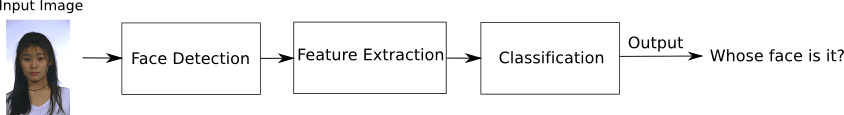
\includegraphics[width=\columnwidth]{ch1/figures/FRS_flowchart.png}
   \caption{The flowchart of three modules of face recognition systems}
    \label{fig:FRSflowchart}
 \end{center}
\end{figure} 
Face detection includes face localisation, segmentation and normalisation, in which a pre-processed face image is obtained from an input scene, either simple or cluttered. Feature extraction derives a representative of the pre-processed face image using a set of features. There are various types of features possibly extracted from the process, such as facial features, statistical appearance-based features, transform coefficient features, algebraic features, etc. In some face recognition systems, there might be a feature selection module between feature extraction and classification. Due to high-dimensionality in the feature space or redundancy among features, such a process is used to select a smaller group of relevant features to represent faces and achieve better recognition performance. Classification is used to assign the above features into one of several categories, \textit{i.e.}, subjects.

Depending on the application context, face recognition can be divided into two scenarios: face verification and face identification. In face verification, an individual who desires to be recognised claims an identity, usually through a personal identification number, an user name, or a smart card. The system conducts a one-to-one comparison to determine whether the claim is true or not, \textit{i.e.}, face verification is to ask a question - ``Does the face belong to a specific person?''. In face identification, the system conducts a one-to-many comparison to establish an individual's identity without the subject to claim an identity, \textit{i.e.}, face identification is to answer the question - ``Whose face is this?''. Throughout this thesis, the generic term \textit{recognition} is used, which does not make a distinction between verification and identification.

\section{Gabor-Boosting algorithm}
Recently, a breakthrough in face detection has been made by Viola and Jones \cite{Viola2001}. Faces are quickly and accurately detected by cascade structured classifiers combined with simple Haar features. In the face detection system, the most significant contribution is the AdaBoost algorithm which selects $200$ most important features from over $180000$ features, and a complex classifier in a cascade structure is built on these important features. The face detector is the most rapid and accurate approach compared to other systems, and it pushes research and development of face detection into a new era. Now many real-time face detection applications, such as those used in digital camera, web cam and mobile phone camera adopt Viola and Jones AdaBoost approach. Facing the big success in face detection, two questions are spontaneously released - ``Can the AdaBoost approach be transplanted into face recognition?'' and if so ``How can the AdaBoost be used in face recognition?''. 
%It leaves the difficulties of face recognition in feature extraction and classification. In the thesis, a face recognition algorithm named \textit{Gabor-Boosting} algorithm is proposed, developed and tested. Gabor wavelet transform is used to extract Gabor wavelet features from face images, Due to very large number of features extracted, AdaBoost is used to select small group of features representing individual's face. After training a classifier with existing faces and their identities, the recognition is done by outputting identities of unknown faces from the classifier. 

This thesis gives an exploration into these two questions. The transplantation of the AdaBoost from face detection into face recognition introduces further sub-questions in feature extraction, feature selection, and classification. These sub-questions are
\begin{itemize}
	\item In face detection, there are only two classes, \textit{i.e.}, face and non-face, so Viola and Jones' work in face detection \cite{Viola2001} is processed using two-class (binary) classification ideas. While, in face recognition, it is more likely there are more than two persons to be discriminated, so that face recognition deals with multiple classes. This prevents the direct transplantation from a two-class environment into a multi-class environment. The solution is to shift face recognition into two-class environments. Hence the sub-question is - ``how can the two-class scenario be established in face recognition?''.
	\item Viola and Jones' approach uses Haar features which are simple so that they can be quickly evaluated. Haar features are sufficient to discriminate differences between face and non-face. However, in face recognition, features are used to discriminate differences between individuals. Obviously, the appearance difference between face and non-face is much larger than the appearance between individuals. Hence, the sub-question is that ``are the Haar features sufficient for face recognition?''. If not, ``what should the substitution be?''.
	\item Within AdaBoost, weak learners (base classifiers)\footnote{Weak learners are the elemental components in AdaBoost training.} are used to evaluate each feature, such that the type of weak learner is a very important factor which determines the performance of AdaBoost. Among the various types of weak learners, ``which types of weak learners are beneficial to improve the performance of face recognition?''.
	\item After the AdaBoost training, a complex classifier is built on weak learners with respect to selected features. The sub-question is: ``is this classifier appropriate for face recognition?''. If not, ``what is the alternative which can be used for recognising human faces?''.
	\item Beside the two-class AdaBoost, there are some multi-class variants of AdaBoost. ``How do these variants fulfil the purpose of multi-class classification from face recognition?''
	\item The AdaBoost approach is very time-consuming \cite{Young2005}. Since images used for face recognition is larger than those images used for face detection in AdaBoost training, the AdaBoost training in face recognition consumes more time than the one in face detection. Hence, there is a sub-question - ``how to reduce the computational time of the AdaBoost training?''.
\end{itemize}

The algorithm described in this thesis is motivated by Viola and Jones' work in face detection \cite{Viola2001}. The algorithm is named \textit{Gabor-Boosting} algorithm, which is proposed, developed and tested. Gabor wavelet transform is used to extract Gabor wavelet features from face images. Due to very large number of features extracted, AdaBoost is used to select a small group of features representing individual's face. After training a classifier with existing faces, the recognition is done by outputting classification results. To evaluate the performance of the Gabor-Boosting face recognition algorithm, the XM2VTS \cite{Matas2000,Messer1999} and FERET \cite{Phillips1997} face databases are used.


%However, there are some differences between face detection and face recognition, which makes applying AdaBoost algorithm difficult on face recognition. In face detection, there are only two subjects, \textit{i.e.}, face and non-face, so Viola and Jones' work in face detection \cite{Viola2001} is processed in a mean of two-class (binary) classification. While, in face recognition, there are many people needed to be recognised, so that face recognition deals with more subjects. The first difficulty is to convert an multiple subjects issue into two subjects issues. In addition, in AdaBoost, weak learners (base classifiers) are used to evaluate each features, such that the type of weak learners is a very important issue which determines the performance of AdaBoost. Different types of weak learners are explored in this thesis, and the optimal type of weak learners is found. In addition, the Gabor-Boosting face recognition is extended from binary classification to multi-class classification with extensions on weak learners and training algorithm. Due to the time-consuming process of AdaBoost, grid computing technology is applied on Gabor-Boosting face recognition, such that the computational time is dramatically reduced. And to evaluate the performance of the Gabor-Boosting face recognition algorithm, the XM2VTS \cite{Matas2000,Messer1999} and FERET \cite{Phillips1997} face databases are used.
In face recognition systems, it is clear that evaluation and benchmarking of the algorithms is crucial. Previous work \cite{Messer1999,Phillips1997,Phillips1998,Phillips2000,Rizvi1998,Rizvi1998fg,Jain2000,Hancock2000,Gauthier2001} on evaluation provides insights into how the evaluation of algorithms and systems can be performed efficiently.  Although great amount of effort has been devoted to face recognition, there are still remains some challenges to be solved such as illumination, head pose, facial expression, occlusion (glasses, sunglasses, scarf, etc), facial hair (beard, mustache, etc.), and ageing. These difficulties make human face appearance in images having very large variations. Therefore, successful face recognition systems have been deployed only under constrained conditions. In this thesis, the face recognition is also deployed under constrained conditions
\begin{itemize}
 \item Illumination is consistent across images
 \item No head pose, but only front-view;
 \item No facial hair and ageing variation, but allowing adequate occlusion (glasses) and facial expression variation.
\end{itemize}
In additional, all images are converted into grey scale.

\section{Thesis Outline}
This thesis is organised as follows: \mbox{Chapter} \ref{ch:review} presents a literature review of face recognition, in which major state-of-the-art techniques of face recognition and face databases are introduced. \mbox{Chapter} \ref{ch:gaboradaboost} gives the background and technical detail of Gabor wavelet transform and AdaBoost. \mbox{Chapter} \ref{ch:FLDAdaBoost} describes the initial Gabor-Boosting face recognition, in which face recognition is converted into two-class classification and Gabor wavelet transform is used to extract human facial features. \mbox{Chapter} \ref{ch:binary} presents a novel weak learner used in AdaBoost training. \mbox{Chapter} \ref{ch:multi} is an extension of the Gabor-Boosting face recognition from a binary domain to a multi-class domain, and also explains how to use grid computing technology to reduce the computational cost of feature selection. The final chapter concludes the work of the Gabor-Boosting algorithm in face recognition, and highlights directions for future work.
\chapter{Literature Review}
\label{ch:review}
Since 1970s, a great progress has been made in the computer based face recognition area. Face recognition has attracted the attention of researchers from various areas. In this chapter, a literature review on face recognition is present. Because the focus of this research is 2-D face recognition, 3-D face recognition is excluded from the chapter. Most recent approaches for face recognition can be divided into two categories: appearance-based face recognition and model-based face recognition. The appearance-based approaches process face images based on statistical analysis of pixel value distributions. The model-based approaches match a general 2-D face model on face images. Furthermore, a $2.5$D approach - 3-D morphable face model is introduced, which adopts a 3-D face model to extract face representations from 2-D face images. 

The chapter is organised as: \mbox{Section} \ref{sec:appearancebased} introduces appearance-based face recognition; \mbox{Section} \ref{sec:modelbased} describes model-based face recognition; \mbox{Section} \ref{sec:3DMM} gives a brief description of 3-D morphable face model; \mbox{Section} \ref{sec:others} briefly introduces rest major approaches. Some popularly used face databases are presented in \mbox{Section} \ref{sec:facedatabase}.

\section{Appearance-Based Face Recognition}
\label{sec:appearancebased}
Many approaches for object recognition are directly applied on 2-D images. A 2-D face image is treated as a high-dimensional vector. They are so called appearance based approaches. Image data can be represented as vectors which are points in a high dimensional vector space. For example, a $128 \times 128$ image can be represented by a vector $x \in \mathcal{R}^{16384}$. In the high-dimensional space, every object is described if it can be depicted in the $128 \times 128$ image. If all vectors in the high dimensional space are the same type of objects, \textit{e.g.}, faces, the natural constraints of the physical world indicate that the vectors will in fact lie in a lower dimensional linear subspace or non-linear manifold. Linear subspace analysis has significantly advanced facial recognition technology, but it does not have sufficient modelling capacity to preserve the variations of the face manifold and distinguish between different persons to achieve high accuracy in face recognition. Recent developments in nonlinear manifold analysis provide more flexibility and modelling capacity to analyse face manifolds. However, the generalisation of nonlinear methods is affected by the number of examples, \textit{e.g.}, there is a small number of face example images in training set, but large variations of facial appearance during the testing. The phenomenon leads incorrect results and overfitting \cite{Zhao2003}.
\subsection{Linear Analysis}
Three classical linear approaches are introduced here, which are Principal Component Analysis (PCA) \cite{Turk1991}, Independent Component Analysis (ICA) \cite{Bartlett1998} and Linear Discriminant Analysis (LDA) \cite{Belhumeur1997,Swet1996}. By projecting a face image to a subspace, the projection coefficients are used as the feature representation of each face image. The classification is performed between the test face image and the training prototype. All representations from these three linear approaches are considered as a linear transformation from the original image vector $x$ to a projection feature vector $y$, \textit{i.e.},
\begin{equation}
 y = W^T x
\end{equation}
where $W$ indicates the transformation.
\subsubsection{PCA}
Principal Component Analysis (PCA) is to find a subspace which accounts for the distribution of face images within the entire image space. The PCA is generated from the Karhunen-Loeve (KL) expansion, which has been widely used for face representation \cite{Kirby1990} and face recognition \cite{Turk1991}. In \cite{Turk1991}, all face images in the training set are collected and composed into a covariance matrix. The eigenvectors and corresponding eigenvalues are generated from the covariance matrix. The eigenvectors are visualised into a two-dimensional array and display ghost face like appearance. Hence, the eigenvectors are also named ``eigenfaces'' as shown in \mbox{Figure} \ref{fig:eigenfacesreview}.
\begin{figure}[ht]
\begin{center}
 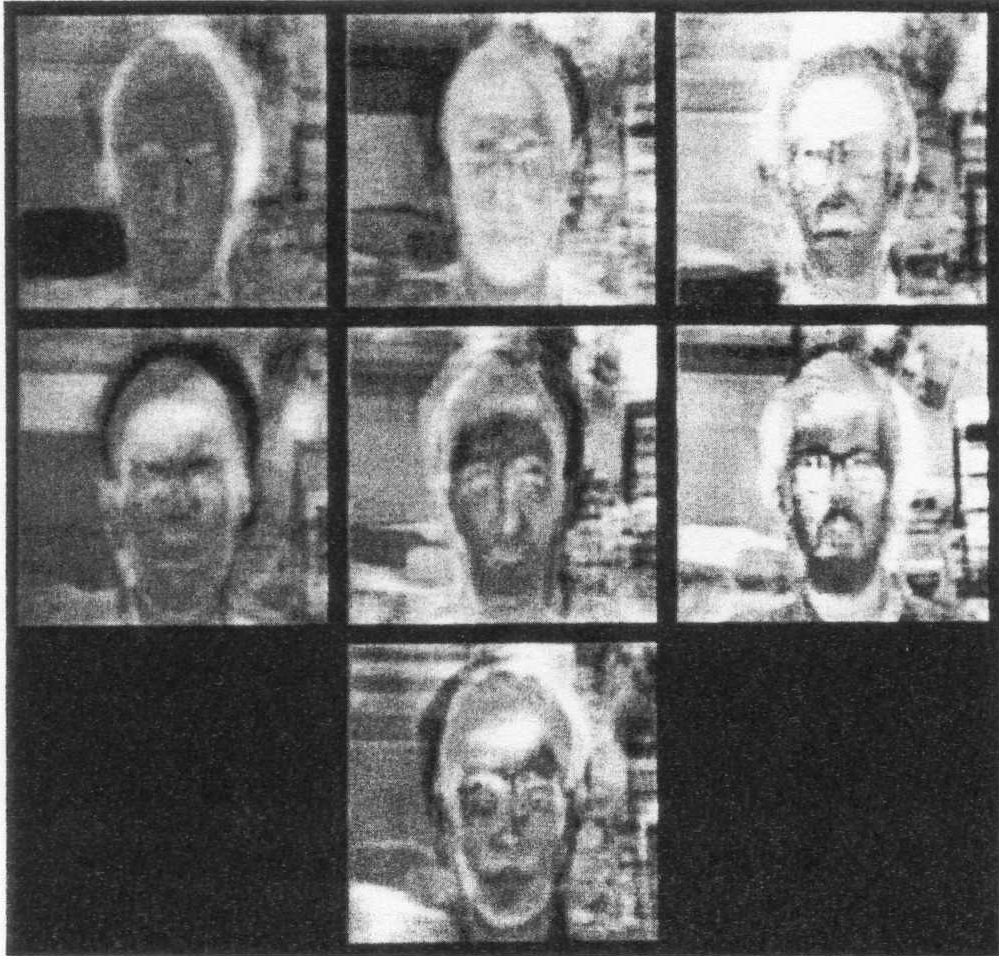
\includegraphics[width=0.8\columnwidth]{ch2/figures/seveneigenfaces.jpg}
\caption{The seven eigenfaces calculated from \cite{Turk1991}}
\label{fig:eigenfacesreview}
\end{center}
\end{figure}  
These eigenfaces span a small subspace in the image space. The subspace is called ``face'' subspace. Given the eigenfaces, every face in the training set can be represented as a vector with a sequence of weights. The weights are obtained by projecting the images into the face subspace by a inner product operation. The testing image is also represented by its vector. The recognition on the PCA approach is done by measuring the Euclidean distance between the testing vector and the existing face vectors in the face subspace. The method is illustrated in \cite{Turk1991} using a large database of $2500$ face images of $16$ subjects with three head orientations, three scales, and three lighting conditions. 

The PCA approach is enhanced in \cite{Pentland1994} by several extensions. The experiments are carried out in a large-scale face database, which contains $7562$ face images of approximately $3000$ people. The first twenty eigenfaces are introduced from a random $128$ images subset. Annotated information on gender, race, approximate age and facial expression is included in the extended approach. A view-based eigenfaces technique is introduced as modular eigenspace so that face recognition can be performed under various poses. The probabilistic analysis is integrated into the eigenface approach in \cite{Moghaddam1997}. The probability density is estimated in the eigenspace. Two types of density estimation are derived from modelling the eigenspaces: a multivariate Gaussian model and a Mixture Gaussian model. By applying Bayes' theorem, the maximum likelihood estimation is used for face detection and face recognition.

Some experiments are conducted to test the performance of the PCA approaches. It is reported that the approach is fair against the illumination change. In \cite{Belhumeur1997}, it is mentioned that by discarding the three most significant eigenvectors, the variation due to lighting is reduced. %Because the first eigenvectors capture the variation due to lighting, the better clustering on the training data is acquired by ignoring these first eigenvectors.

\subsubsection{ICA}
Like the PCA, Independent Component Analysis (ICA) is also a linear transformation. The PCA is to find the ranked principle components which describe the variation, however the ICA is to find the independent components by maximising the statistical independence between these estimated components. The independence of the components is measured by maximising Non-Gaussian distribution. The popular algorithms to computing ICA include infomax \cite{Bell1995}, FastICA \cite{Hyvarinen1999,Hyvarinen2001}, and JADE \cite{Cardoso1996}.

The ICA is a generalised version of the PCA, and the PCA can be derived as a special case of ICA, as Gaussain component models are used. The difference betwen ICA and PCA is illustrated in \mbox{Figure}.\ref{fig:icaVSpca}.
\begin{figure}[ht]
 \begin{center}
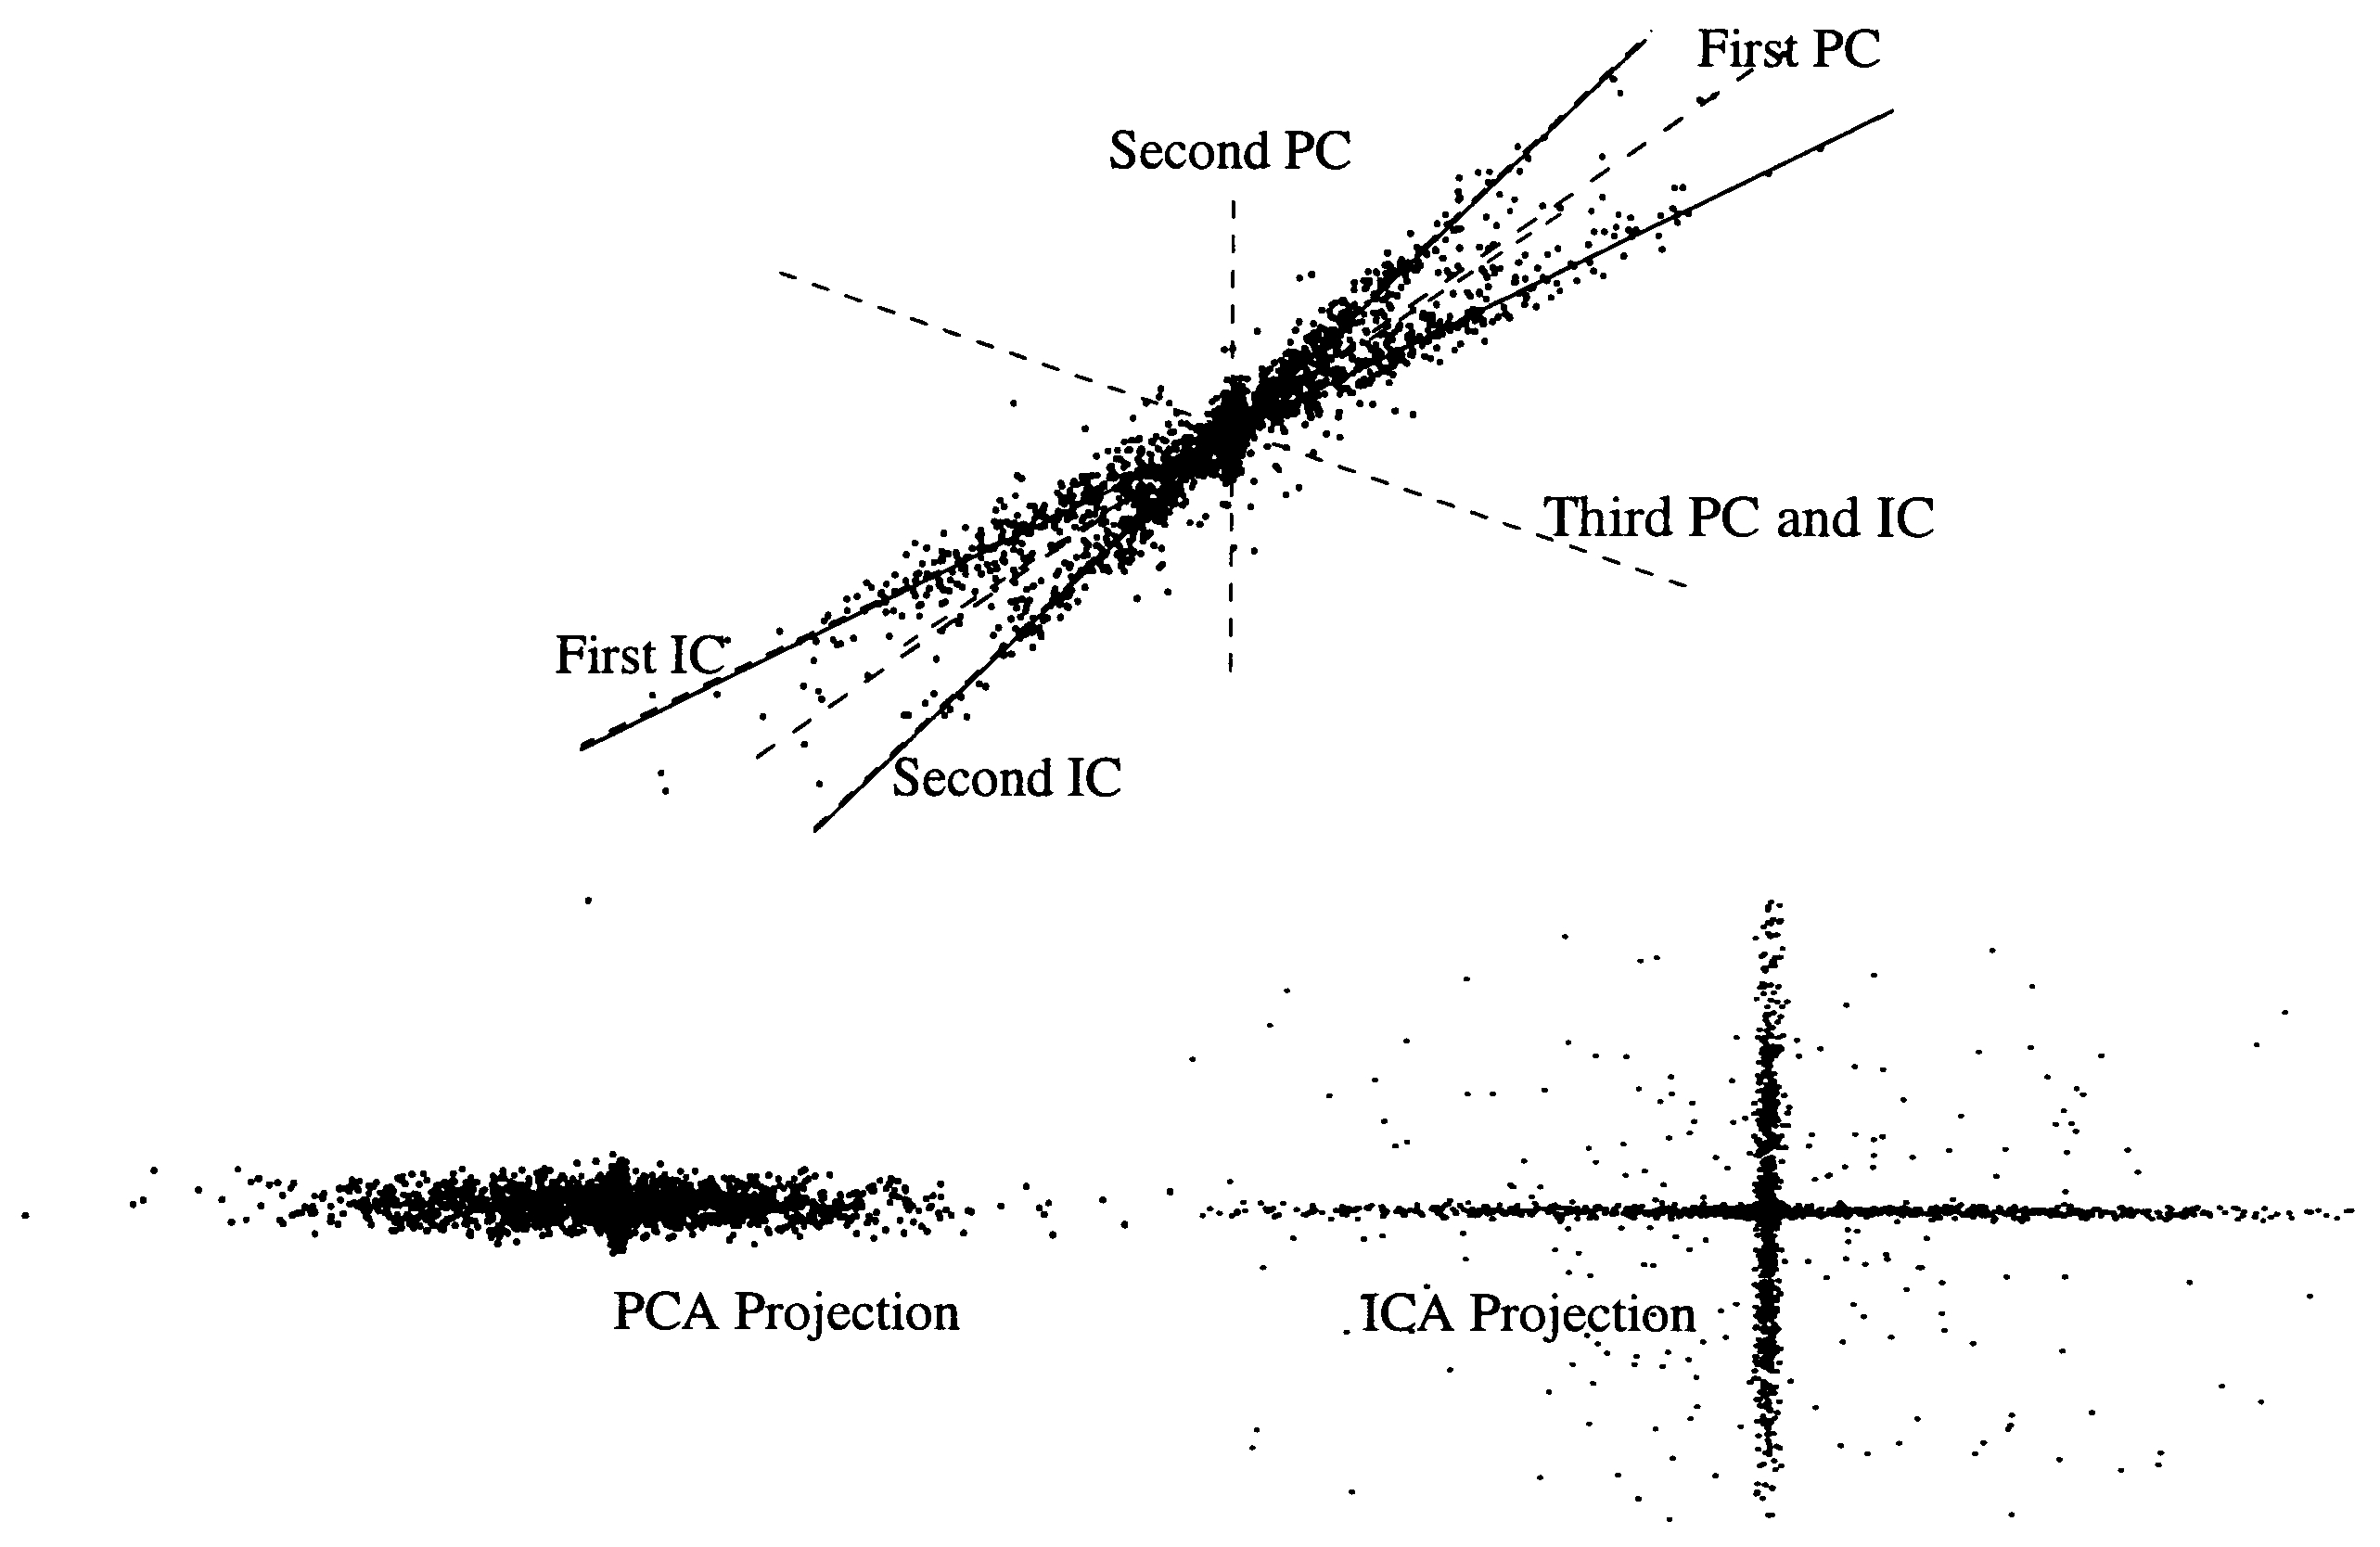
\includegraphics[width=0.7\columnwidth]{ch2/figures/icaVSpca.jpg}
  \caption{The difference between ICA and PCA \cite{Bartlett2002}.}
\label{fig:icaVSpca}
 \end{center}
\end{figure} 
There are 3-D data examples residing in a 3-D axes space. The Independent Component (IC) and Principal Component (PC) construct different coordination systems. The PC axes are orthogonal while the IC axes are not. If only two components are allowed, ICA chooses a different subspace than PCA. In the PCA projection, the data are sparsely distributed on the first PC, but closely clustered on the second PC. In ICA projection, the data are both sparsely distributed on the first and second ICs. Since the ICA axes are nonorthogonal, relative distance between points are different in PCA than in ICA. In \cite{Baek2002}, a comparison between ICA and PCA is given. It shows that the ICA outperforms PCA on a human face recognition task when both using same distance metric, \textit{i.e.}, cosine angle. However, when the L1 norm is adapted, the PCA significantly outperforms ICA.

In \cite{Bartlett2002}, ICA was applied on face recognition in the \mbox{FERET} database under two architectures. In the first architecture, the images are treated as random variables and the pixels are treated as outcome. The spatially local basis images for the faces are found as shown in \mbox{Figure} \ref{fig:25ICs1}.
\begin{figure}[t]
 \begin{center}
  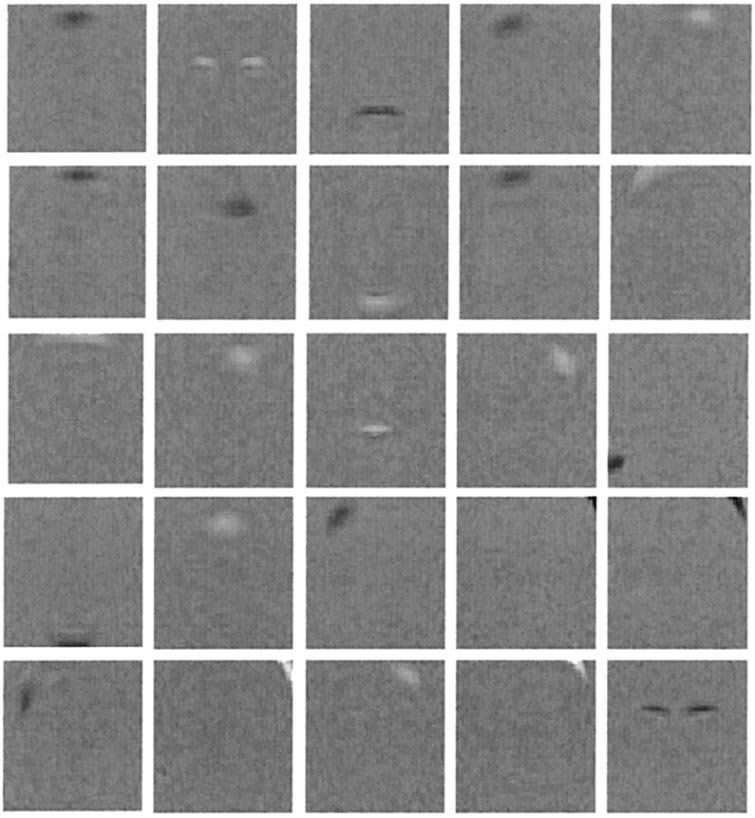
\includegraphics[width=0.7\columnwidth]{ch2/figures/25ICsArch1.jpg}
  \caption{Twenty-five image sets obtained by Architecture I in \cite{Bartlett2002}}
  \label{fig:25ICs1}
 \end{center}
\end{figure} 
In the second architecture, the pixels are treated as random variables, and the images as outcome. A factorial face code is produced in the second architecture. The ICA separates the high-order moments of the input, while the second order moments are utilised in the PCA. The ICA factorial code representation is illustrated in \mbox{Figure} \ref{fig:25ICs2}.
\begin{figure}[ht]
 \begin{center}
  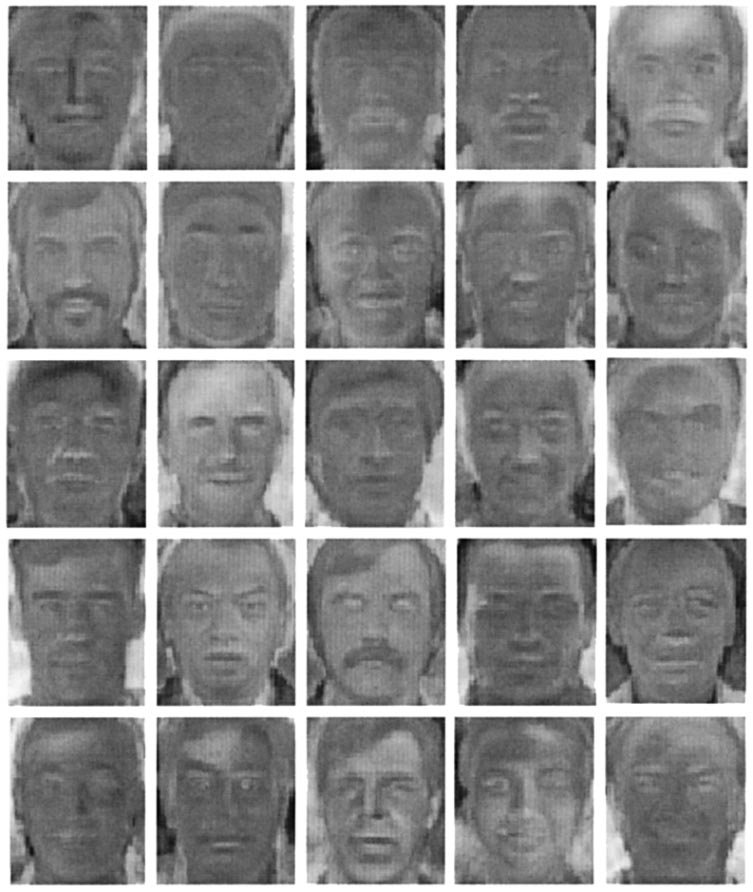
\includegraphics[width=0.7\columnwidth]{ch2/figures/25ICsArch2.jpg}
  \caption{The basis images for the ICA-factorial representation obtained with Architecture II in \cite{Bartlett2002}}
  \label{fig:25ICs2}
 \end{center}
\end{figure} 

Liu and Wechsler \cite{Liu2003} present an independent Gabor feature (IGF) method and its application to face recognition. The method derives independent Gabor features in the feature extraction stage, and an IGF feature-based probabilistic reasoning model (PRM) classification method is developed in the pattern recognition stage. The IGF method is firstly to acquire a Gabor feature vector from a set of Gabor wavelet representations of face images, then to reduce the dimensionality of the vector by means of principal component analysis, and finally to define the independent Gabor features based on the ICA. Experiments on face recognition are carried out by using the FERET and the ORL datasets. The images vary in illumination, expression, pose, and scale. The IGF method achieves $98.5\%$ correct face recognition accuracy when using 180 features for the FERET dataset, and $100\%$ accuracy for the ORL dataset using $88$ features. The approach is extended with enhanced ICA \cite{Liu2004smc}.
\subsubsection{LDA}
Both PCA and ICA are unsupervised methods that yield a set of linear features of a particular dimension, but there is no consideration if this set of features is good for classification. In the PCA, the examples' cluster is maximised not only between different class clusters but also within the same class cluster. The PCA does not take classes into account when there are more than one class in a dataset. This leads to significant problems. For the data set on \mbox{Figure} \ref{fig:PCAbada}, one class is indicated by circles and the other by stars. 
\begin{figure}[ht]
 \begin{center}
  %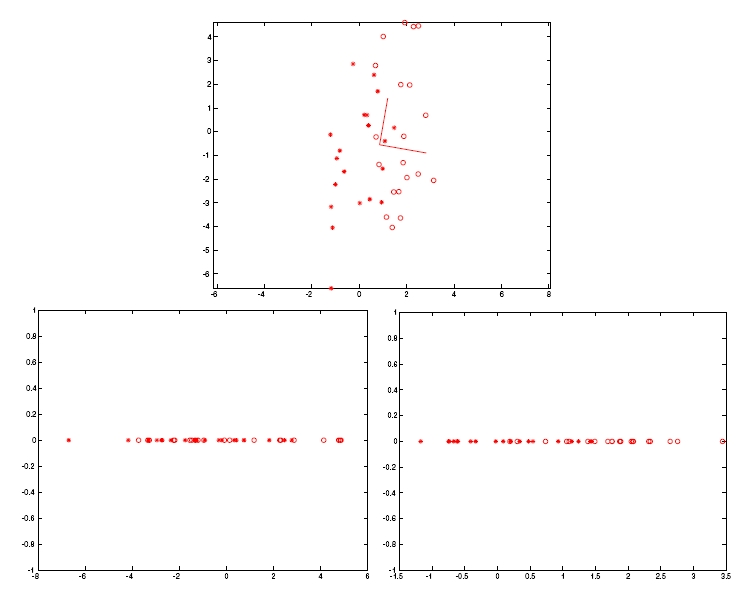
\includegraphics[width=\columnwidth]{ch2/figures/LDAvsPCA.jpg}
  \subfigure[The original 2D data set contains two classes]{\label{fig:PCAbada}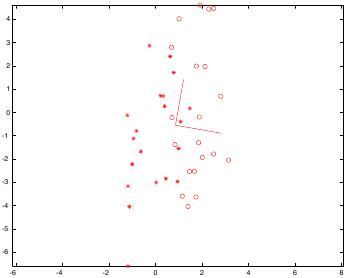
\includegraphics[width=0.45\columnwidth]{ch2/figures/LDAvsPCA_a.jpg}}\\
  \subfigure[The data are projected onto the first PC.]{\label{fig:PCAbadb}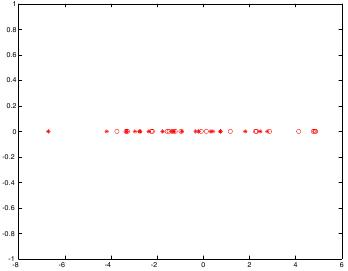
\includegraphics[width=0.45\columnwidth]{ch2/figures/LDAvsPCA_b.jpg}}
  \subfigure[The data are projected onto the second PC.]{\label{fig:PCAbadc}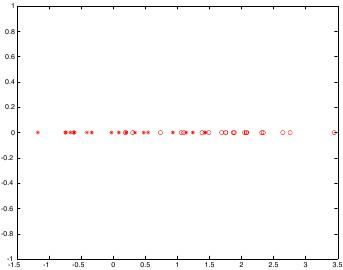
\includegraphics[width=0.45\columnwidth]{ch2/figures/LDAvsPCA_c.jpg}}
 \end{center}
\caption{The PCA has no consideration for classification purpose. \cite{Forsyth2003}}
\label{fig:PCAbad}
\end{figure} 

The PCA would suggest projection onto a vertical axis, which captures the variance in the dataset, but cannot be used to discriminate it from the axes obtained by PCA, which are overlaid on the data set. The bottom of \mbox{Figure} \ref{fig:PCAbad} shows the projections onto those two axes. \mbox{Figure} \ref{fig:PCAbadb} is the projection onto the first PC, which has higher variance, but separates the classes poorly. \mbox{Figure} \ref{fig:PCAbadc} shows the projection onto the second PC, which has significantly lower variance and gives better separation. \mbox{Figure} \ref{fig:PCAbad} shows the first PC would produce a bad classification, while the second PC would produce a good classification, despite the factor that the second PC does not scatter the data.

Linear Discriminant Analysis (LDA) is a statistical method to classify examples into different classes based on a set of measurements of examples. The LDA applied in face recognition is very successful, because LDA is originally for classification, \textit{i.e.}, the LDA is a supervised learning approach. In LDA, the purpose is to maximise the discrimination between different classes, and recognition can be apparently done based on this. The LDA also constructs a subspace that is constructed by the selected components. The LDA training is carried out by using scatter matrices. The method selects a set of features in such a way that the ratio of the between-class scatter and the within-class scatter is maximised. The between-class scatter matrix is defined as
\begin{equation}
 S_B = \sum_{i=1}^c N_i (\mu_i-\mu)(\mu_i-\mu)^T
\end{equation}
and the within-class scatter matrix is defined as
\begin{equation}
 S_W = \sum_{i=1}^c \sum_{x_k \in X_i} (x_k-\mu_i) (x_k - \mu_i)^T
\end{equation}
where $\mu_i$ is the mean image of class $X_i$, and $N_i$ is the number of examples in class $X_i$, and $c$ is the number of classes. If the scatter matrix $S_W$ is nonsingular, the optimal projection $W_{opt}$ is chosen as the matrix with orthonormal columns which maximises the ratio of determinant of the between-class scatter matrix of the projected examples to the determinant of the within-class scatter matrix of the projected examples,\textit{ i.e.}
\begin{equation}
 W_{opt} = \arg \max_W \frac{|W^T S_B W|}{|W^T S_W W|}
\end{equation}
and the projection $W_{opt}$ can expressed as
\begin{equation}
 W_{opt} = [w_1\quad w_2 \quad \ldots \quad w_m]
\end{equation}
where $\{w_i|i=1,2,\ldots,m\}$ is a set of generalised eigenvectors of $S_B$ and $S_W$ corresponding to the $m$ largest generalised eigenvalues. Because an upper bound on $m$ is $c-1$, there are $c-1$ nonzero components.

However, in some real applications, the number of images in the training set $N$ is normally much smaller than the number of pixels in each image $n$, so that the within-class scatter matrix $S_W$ tends to be always singular. The phenomenon is called \textit{small sample size} problem \cite{Fukunaga1990}. 

To overcome the small sample size problem, different methods have been proposed in face recognition literature. 

Some methods reduce the dimension of the original sample space, which has been demonstrated to contain considerable discriminative information. In \cite{Belhumeur1997}, a method called ``Fisherfaces'' is proposed. The method is achieved by using PCA to reduce the dimension of feature space to $N-c$, and then apply the LDA to reduce the dimension further to $c-1$.  In \cite{Zhao1998}, the images are firstly preprocessed by photometrical and geometrical techniques, secondly projected by PCA, then projected by LDA, and finally using Euclidean metric and weight mechanism to make decision. These traditional solutions to the small sample size problem require the incorporation of a PCA step into the LDA framework. PCA is used as a preprocessing step for dimensionality reduction so as to discard the null space of the within-class scatter matrix $S_W$ of the training data set, and then LDA is performed in the lower dimensional PCA subspace.

The PCA+LDA methods discard a null space of the within-class scatter matrix $S_W$, and the null space may contain significant discriminative information. In \cite{Chen2000}, an LDA-based method that makes use of the null space of $S_W$ is proposed. All the examples are firstly projected onto the null space of $S_W$, where the within-class scatter is zero, and then the optimal discriminant vectors of LDA are those vectors that can maximise the between-class scatter. Examples are processed directly in the original high-dimensional input space avoiding the loss of significant discriminatory information. Hence, the approach is called Direct LDA (D-LDA) or Null-space LDA. Various approaches \cite{Huang2002,Lu2003,Wu2004,Cevikalp2004,Fan2004} are developed based on D-LDA and are endeavoured to model and calculate the null space. The main drawback of these approaches is that the computational complexity of determining the null space $S_W$ is very high due to the high dimension in $S_W$ itself.

In \cite{Belhumeur1997}, there is a comparative performance analysis carried out on four methods, which are a correlation-based method, a variant of the linear subspace method \cite{Shashua1994}, a PCA method, and a LDA method. The four methods are tested on the Harvard database \cite{Hallinan1995} and the Yale database \cite{Georghiades2001}. The conclusions are drawn such as
\begin{enumerate}
 \item All linear methods perform well if images in training set are similar to images in testing set.
 \item The LDA method appears to be the best at extrapolating and interpolating over illuminant changing.
 \item The largest three principal components does not improve the performance of the PCA method, so that removing these components can gain the performance.
 \item The best number of selected principal components (PCs) is about $45$.\footnote{the conclusion is corresponding to the experiment in \mbox{Appendix} \ref{apx:pcaca} where the best number is $49$ very close to $45$.} The performance drops, when more than $45$ components are used, 
 \item The LDA method appears to be the best on illuminance changing, but suffers when confronted with various facial expression.
\end{enumerate}

Recently, some progress has been made on linear subspace approaches. In two-dimensional PCA \cite{Yang2004}, an image is represented as a 2-D matrix instead of as a vector, and a two-dimensional PCA algorithm for face recognition is developed. Similar to two-dimensional PCA, Kong \textit{et al.} \cite{Kong2005} generalised the conventional LDA into 2-D Fisher discriminant analysis and applied it to face recognition.

\subsubsection{Summary on linear approaches}
In PCA, the eigenface coefficients in face representation are the most descriptive among the three major linear approaches. Due to many established algorithms or source codes, the PCA is easy to be implemented, and also servers as a baseline algorithm in face recognition. However, the PCA is not discriminative for class separation, since it does not take any class information into account. The ICA utilises higher-order statistics in the training data instead of only the second-order statistics in PCA, but there is no general closed-form solution in ICA. In addition, iterative methods, which are used to obtain the ICA representation, cause large amount of computational time. The LDA utilises the class information in the derivation of the representation for the face recognition task, and is a classification problem instead of subspace represetnation problem. The recognition rate in LDA is the highest among the three major linear approaches. However, due to the small sample size problem, the within-class scatter matrix becomes singular, which leads to poor performance on LDA. In \mbox{Appendix} \ref{apx:pcaca}, the experiment of PCA and Canonical Variate is presented, which is also corresponding to the findings in the chapter. 


\subsection{Non-linear Analysis}
In non-linear analysis, it is assumed that objects reside in non-linear structures. The non-linear structures are normally described as \textit{manifold}. A manifold is an abstract mathematical space in which every point has a neighbourhood which resembles an Euclidean space, but in which the global structure may be more complicated. In a one-dimensional manifold (or one-manifold), every point has a neighbourhood that looks like a segment of a line. Examples of one-manifolds include a line, a circle, and two separate circles. In a two-dimensional manifold, every point has a neighbourhood that looks like a disk. Examples include a plane, the surface of a sphere, and the surface of a torus. Manifolds are important objects in mathematics and physics because they allow more complicated structures to be expressed and understood in terms of the relatively well-understood properties of simpler spaces.

The face manifold is more complicated than that in linear subspace models. Linear subspace approaches approximate the non-linear manifold in a linear way. Therefore, non-linear manifold modelling is directly investigated to find the corresponding non-linear manifold. The comparison between linear approach and non-linear approach is given in \mbox{Figure} \ref{fig:linearvsnon-linear}.
\begin{figure}[ht]
\begin{center}
 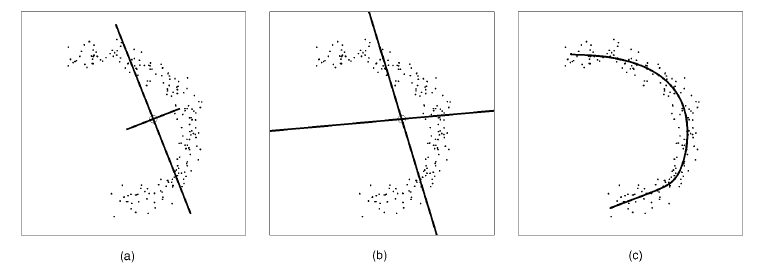
\includegraphics[width=\columnwidth]{ch2/figures/linearvsnonlinear.jpg}
\caption{(a) PCA basis (linear, ordered, and orthogonal). (b) ICA basis (linear, unordered, and nonorthogonal). (c) Principal Curve (parameterised nonlinear manifold). \cite{Moghaddam2002}}
\label{fig:linearvsnon-linear}
\end{center}
\end{figure} 
In \mbox{Figure} \ref{fig:linearvsnon-linear}(a), the principal component vectors are obtained with a toy data set corresponding to an essentially one-dimensional manifold. The first and second components are orthogonal to each other. In \mbox{Figure} \ref{fig:linearvsnon-linear}(b), the ICA produces two unordered nonorthogonal components, one of which is roughly aligned with the first principal component. \mbox{Figure} \ref{fig:linearvsnon-linear}(c) is an example of a principal curve, which is the simplest methods for principal manifold. The principal curve yields a compact and relatively accurate representation of the toy data. Also it displays that for capturing the non-linear manifold, non-linear approach is superior to linear subspace approach.

The classical non-linear approaches such as Kernel PCA \cite{Scholkopf1998}, Kernel LDA \cite{Yang2002}, Kernel ICA  \cite{Bach2002} and Isomap embedding \cite{Tenenbaum2000} are introduced in this subsection.
\subsubsection{Kernel PCA}
The kernel PCA (KPCA) \cite{Scholkopf1998} is to apply an non-linear mapping from the input space $\mathcal{R}^N$ to the feature space $\mathcal{R}^L$ by $\Psi(x): \mathcal{R}^N \rightarrow \mathcal{R}^L$, where $L$ is larger than $N$ and possibly infinite. The mapping $\Psi(x)$ is made by the use of kernel functions meeting the Mercer's theorem \cite{Vapnik1995}
\begin{equation}
 k(x_i,x_j)= (\Psi(x_i)\cdot \Psi(x_j)),
\end{equation}
where the kernel function $k(x_i,x_j)$ in the input space corresponds to dot-products in the higher dimensional feature space. Because computing a covariance matrix is based on dot product, PCA in the feature space can be formulated without direct computation of $\Psi(x)$. Assuming that the mean of the projection of the examples in the feature space is equal to zero, the covariance is given by
\begin{equation}
 \Sigma_K = \langle \Psi(x_i) \Psi(x_i)^T  \rangle
\end{equation}
with resulting eigenvector equation $\lambda V= \Sigma_K V$. The eigenvector solutions $V$ exist with coefficients $\{\omega_i\}$ such that $V=\sum_{i=1}^{T}\omega_i \Psi(x_i)$, where $T$ is the total number of training examples. The equivalent eigenvalue problem can be formulated as
\begin{equation}
 T \lambda \omega = K \omega
\end{equation}
where $\omega$ is a set of $\{\omega_i\}$, and $K$ is a $T\times T$ matrix. The KPCA principal components of any input example can be computed with simple kernel computation against the data set. The $n$-th principal component $y_n$ of the example $x$ is given by
\begin{equation}
 y_n = ( V^n \cdot \Psi(x)) = \sum_{i=1}^T \omega_i^n k(x,x_i)
\end{equation}

Moghaddam \cite{Moghaddam2002} extends the KPCA approach with a \textit{maximum a posteriori} (MAP) matching rule using a Bayesian similarity measure derived from dual probabilistic subspaces. In \cite{Zhou2004}, the KPCA application in face recognition is demonstrated and the recognition performance indicates its advantage over other traditional subspace approaches.
\subsubsection{Kernel LDA}
The Kernel Fisher Linear Discriminant (KFLD) \cite{Yang2002} is similar to KPCA. The projected examples are centred in the feature space. The within-class and between-class scatter matrices are denoted by $S_W^{\Psi}$ and $S_B^{\Psi}$, and applying FLD in kernel space. The eigenvalues $\lambda$ and eigenvectors $w^{\Psi}$ of
\begin{equation}
 \lambda S_W^{\Psi} \omega^{\Psi} = S_B^{\Psi} w^{\Psi}
\end{equation}
which can be obtained by
\begin{equation}
 W_{opt}^{\Psi} = \arg \max_{W^{\Psi}} \frac{|(W^{\Psi})^T S_B^{\Psi} W^{\Psi}|}    {|(W^{\Psi})^T S_W^{\Psi} W^{\Psi}|}  
\end{equation}
where $W_{opt}^{\Psi} =[w_1^{\Psi}\quad w_2^{\Psi}\quad \ldots \quad w_m^{\Psi}]$ is the set of generalised eigenvectors corresponding to the $m$ largest generalised eigenvalues.

For given classes $t$ and $u$ and their examples, the kernel function is defined by
\begin{equation}
 (K_{rs})_{tu} = k(x_{tr}, x_{us}) = \Psi(x_{tr})\cdot \Psi(x_{us}) = \Psi(x_{tr})^T \Psi(x_{us})
\end{equation}
Let $K$ be an $m\times m$ matrix, where $K_{tu}$ is a matrix composed of dot product in the feature space $\mathcal{R}^L$.
From the theory of reproducing kernels, any solution $w^{\Psi} \in \mathcal{R}^L$ must lie in the span of all training examples in $\mathcal{R}^L$. The solution is obtained by solving the following equation 
\begin{equation}
 \lambda K K \alpha = K Z K \alpha
\end{equation}
where $Z$ is an $m\times m$ block diagonal matrix.
The $\Psi(x)$ is projected into a lower dimensional space spanned by the eigenvectors $w^{\Psi}$ in a way similar to KPCA. 

In \cite{Yang2002}, KFLD achieves lower error rates than those in PCA, LDA, ICA, KPCA approaches in face recognition.

\subsubsection{Kernel ICA}
The kernel based ICA is proposed by Bach and Jordan \cite{Bach2002}, who use contrast functions based on canonical correlations in a reproducing kernel Hilbert space to develop a new class of ICA algorithm.

\subsubsection{ISOMAP Embedding}
Isometric Feature Mapping (ISOMAP) \cite{Tenenbaum2000} is a global optimal, and asymptotic method in which convergence guarantees the flexibility to learn a broad class of nonlinear manifolds. The approach seeks to preserve the intrinsic geometry of the data, as captured in the geodesic manifold distances between all pairs of data points. The core is to estimate the geodesic distance between far away points, given only input-space distances. For neighboring points, input space distance provides a good approximation to geodesic distance. For faraway points, geodesic distance can be approximated by adding up between neighboring points. These approximations are computed efficiently by finding shortest path in a graph with edges connecting neighboring data points. \mbox{Figure} \ref{fig:ISOMAP}  describes how ISOMAP exploits geodesic paths for nonlinear dimensionality reduction on the ``Swiss roll'' data set.
\begin{figure}[ht]
 \begin{center}
  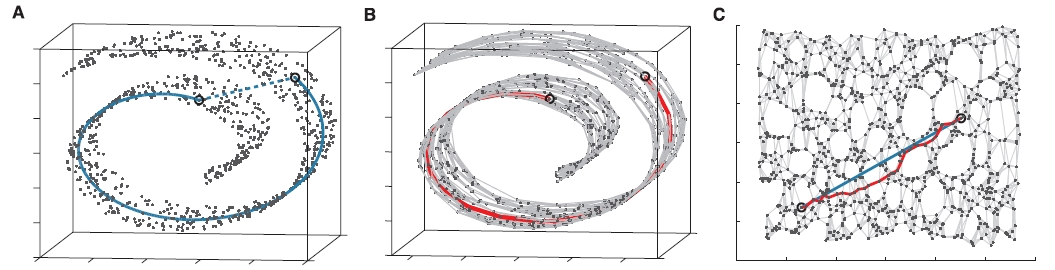
\includegraphics[width=\columnwidth]{ch2/figures/ISOMAP.jpg}
  \caption{ISOMAP exploits geodesic paths on the ``Swiss roll'' data set.}
  \label{fig:ISOMAP}
 \end{center}
\end{figure} 
In \mbox{Figure} \ref{fig:ISOMAP}(A), there are two arbitrary points (circled) on a nonlinear manifold. The Euclidean distance between them in the high dimensional input space may not accurately reflect their intrinsic similarity, as measured by geodesic distance along the low-dimensional manifold (length of solid curve). In \mbox{Figure} \ref{fig:ISOMAP}(B), the neighbourhood graph $G$ constructed in ISOMAP with $k$-near neighour with $k=7$ on $1000$ data points. It allows an approximation (red segments) to the true geodesic path to be computed. \mbox{Figure} \ref{fig:ISOMAP}(C) shows the two-dimensional embedding recovered by ISOMAP, which best preserves the shorest path distances in the neighbourhood graph. Straight lines in the embedding represent simpler and cleaner approximations to the true geodesic paths than do the corresponding graph path (red lines).

Yang \cite{Yang2002ICIP} presents an extended ISOMAP method that utilise LDA for pattern classification, and shows promising results compared with other best classification methods.

\subsection{Bayesian Framework}
In some face recognition systems, a probabilistic similarity between faces is measured based on Bayesian framework. In \cite{Moghaddam1997, Moghaddam2000}, the eigenface method is proposed based on simple subspace norms with a probabilistic model. The similarity between faces on a standard Bayesian analysis of image is divided into two classes: \textit{intra-personal difference} and \textit{extra-personal difference}. The intra-personal difference measures the variations in the appearance of the same person with different expressions and illuminations, while the extra-personal difference measures the variations in the appearance between different persons. The high-dimensional probability density functions for each class are estimated from training data with either single modal density or multimodal densities. The similarity of faces is measured based on \textit{maximise a posteriori }(MAP) probability to decide intra-personal difference or extra-personal difference. In \cite{Moghaddam2000}, Moghaddam \textit{et al.} also proposed an face alignment process (see \mbox{Figure} \ref{fig:facealign}) used in face recognition systems.
\begin{figure}[ht]
 \begin{center}
  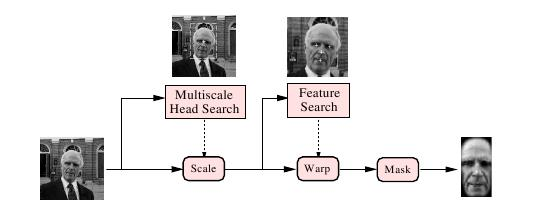
\includegraphics[width=\columnwidth]{ch2/figures/facealignsystem.jpg}
  \caption{The face alignment process \cite{Moghaddam2000}}
  \label{fig:facealign}
 \end{center}
\end{figure} 
\subsection{Summary on appearance-based approaches}
Over the past $30$ years, appearance-based face recognition has been explored and many efficient algorithms have been developed. However, current appearance-based approaches in face recognition systems encounter difficulties in practice due to the small number of available training face images and complex facial variations in the test images. Human face appearance has a number of variations in different lighting conditions, head pose, and facial expressions. There are only small number of images avaliable for training. If a sufficient amount of representative data is not available, a switch \cite{Martinez2001} from non-discriminant techniques to discriminant techniques may lead to poor system performance. Some other techniques, such as face synthesis, can obtain additional training images from the available training data. These techniques \cite{Zhao2000} are helpful to enhance the performance of face recognition. Furthermore, the techniques such as classifier fusion \cite{Lu2003fusion} can help to enhance the performance of face recognition systems.

\section{Model-Based Face Recognition}\label{sec:modelbased}
The model-based approaches in face recognition is to build a model of the human face, which is a flexible model capable to capture facial variations. The prior knowledge of a human face is applied in building up the model, such as the distance between relative feature positions among facial landmarks (i.e. eyes, nose, etc). Early approaches \cite{Galton1888,Bledsoe1964,Kelly1970,Kanade1977} are developed based on localising positions of facial landmarks. A recent feature-based system, \textit{i.e.}, Elastic Bunch Graph Matching \cite{Wiskott1997}, is to find the topological relationship and feature values. Active Shape/Appearance Model \cite{Cootes1996} uses shape and texture information. The model-based approaches usually contain three stages: model construction, model fitting/matching, and recognition.
\subsection{Early Approaches}
The original approach for face recognition can be traced to 1888 by Galton \cite{Galton1888}. A framework for face recognition is proposed by collecting facial profiles. The facial profiles are drawn into curves as shown in \mbox{Figure} \ref{fig:Galton1888}, and the norm of these curves are discovered. The facial profiles are classified by measuring their deviations from the norm.
\begin{figure}[ht]
 \begin{center}
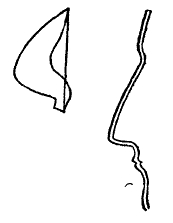
\includegraphics[scale=0.5]{ch2/figures/Galton1888.jpg}
  \caption{The curves depicted from facial profiles \cite{Galton1888}}
\label{fig:Galton1888}
 \end{center}
\end{figure} 

Following the idea, many face recognition systems have been developed in 60s to 70s of 20th century due to the employment of computers. In \cite{Bledsoe1964}, facial feature points are manually located by human operators. The positions of these points are feed to nearest neighbour or other classifiers for identifying the label of the test image. A similar face recognition system without human intervention is developed by Kelly \cite{Kelly1970}. The recognition is determined by measurements of features, \textit{e.g.}, width of head, distance between eyes, distance from top of head to eyes, distance between eyes to nose, and distance from eyes to mouth. In \cite{Kanade1977}, facial feature points are located in two stages: coarse-grain stage and fine-grain stage. The coarse-grain stage simplifies the succeeding differential operation and feature finding algorithms. The fine-grain stage confines the processing to four smaller regions. The two stage processes are depicted in \mbox{Figure} \ref{fig:Kanade1977}. 
\begin{figure}[ht]
  \begin{center}
  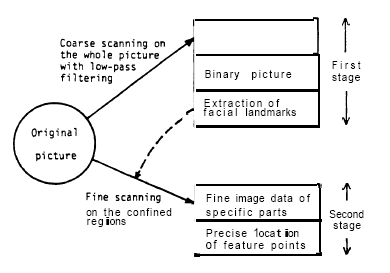
\includegraphics[width=0.8\columnwidth]{ch2/figures/kanade1977.jpg}
   \caption{Two-stage process for computer measurement of features of human-face photographs. \cite{Kanade1977}}
 \label{fig:Kanade1977}
  \end{center}
\end{figure}
 
Human face is characterised by geometrical parameterisation. These parameters may be the distance or angles between key feature points on face images. These methods are limited by storage capacity and computational speed, and are not popular now.

\subsection{Elastic Bunch Graph Matching}
Elastic Bunch Graph Matching (EBGM) is originated from Dynamic Link Architecture (DLA) framework \cite{Lades1993}. The DLA started by computing Gabor wavelets, and then it performs a flexible template comparison between resulting image decompositions using graph-matching. Object recognition is formulated as elastic graph matching, which is operated by loose optimisation of a cost function. \mbox{Figure} \ref{fig:DLA} shows the example of DLA model and graph matching on human faces.
\begin{figure}[ht]
 \begin{center}
  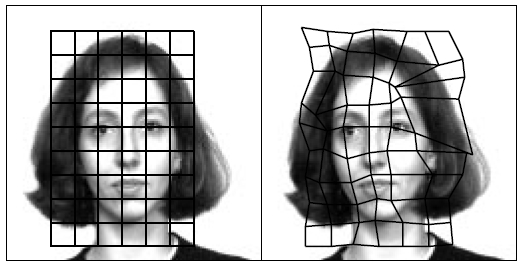
\includegraphics[width=0.77\columnwidth]{ch2/figures/DLAmodel.jpg}
  \caption{The example of DLA model and graph matching.\cite{Lades1993}}
  \label{fig:DLA}
 \end{center}
\end{figure} 
The left part displays the example of a stored object - human face, represented by a rectangular grid form of model graph. The vertices are labeled with magnitude coefficients of Gabor wavelets. The matching begins with an undistorted copy of the object graph. The right part displays the results after grid graph matched with face images. The graph is firstly positioned by ``global moves'', and it is then modified by individual Gabor wavelets diffusion. The grid demonstrates that the graph is accepted as the best match.
\subsubsection{Graphs}
The model of EBGM approach is called \textit{labeled graph}. A labeled graph $\mathcal{G}$ contains $N$ nodes connected by $E$ edges. The nodes are called \textit{fiducial points}, which are facial landmarks, \textit{e.g.}, the pupils, the corners of the mouth, the tip of the nose, the top and bottom of the ears. The graph is object-adapted. If the object is represented by human faces, the geometrical structure is adapted to the structure of human faces as shown in \mbox{Figure} \ref{fig:graphs}.
\begin{figure}[ht]
 \begin{center}
  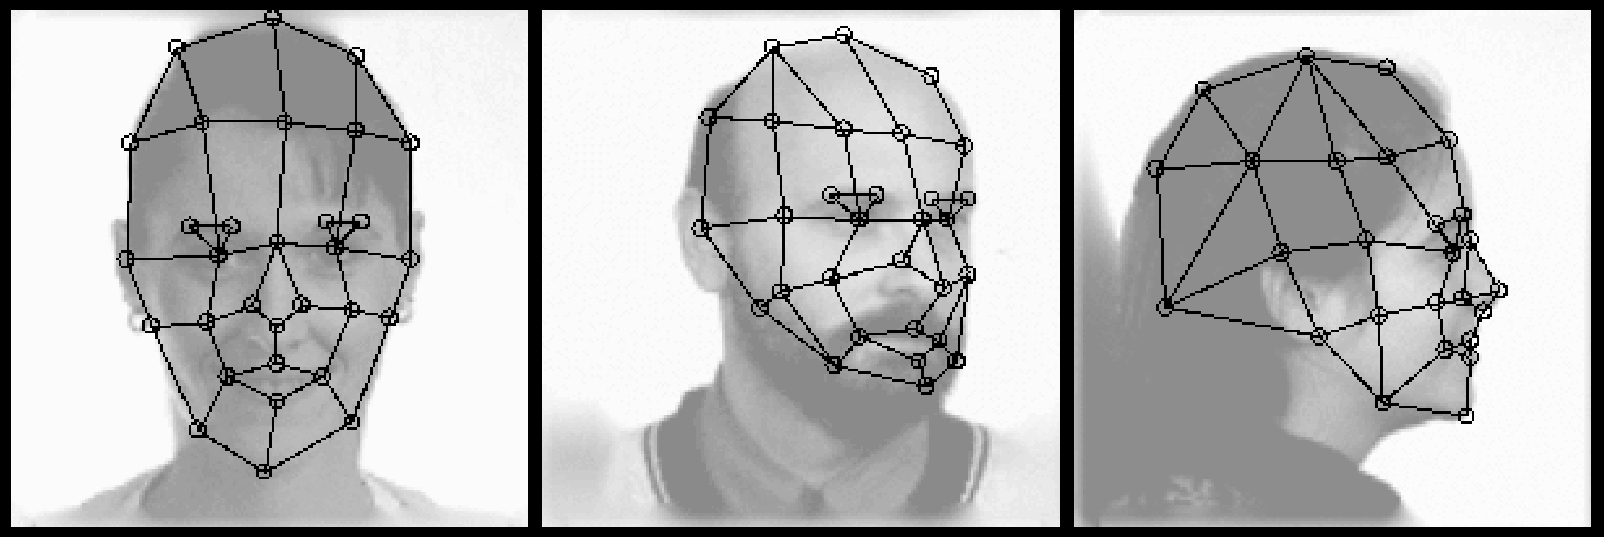
\includegraphics[width=0.77\columnwidth]{ch2/figures/EBGMgrid.jpg}
  \caption{Multiview faces overlaid with labeled graphs. \cite{Wiskott1997}}
  \label{fig:graphs}
 \end{center}
\end{figure} 
There are face-adapted graphs for different poses. These nodes are positioned automatically by elastic bunch graph matching. Each node is also known as a jet. A jet is based on a wavelet transform, defined as a convolution of the image with a family of Gabor kernels. Hence, a jet $J$ is defined as the set of $40$ complex Gabor wavelet coefficients obtained for one image pixel. These $40$ Gabor wavelets are varied with $5$ different spatial frequencies and $8$ orientations. The jet containing the imaginary and magnitude of the coefficients from the convolution is demonstrated in \mbox{Figure} \ref{fig:AGaborJet}.
\begin{figure}[ht]
 \begin{center}
  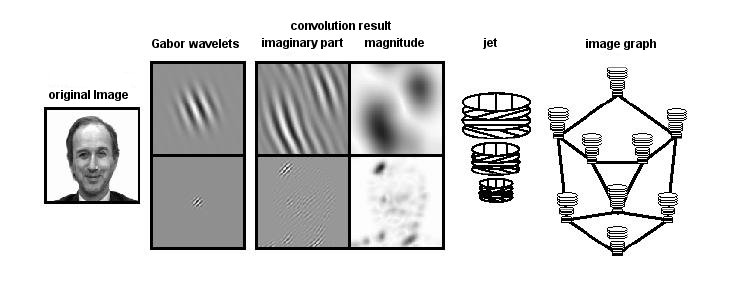
\includegraphics[width=\columnwidth]{ch2/figures/AJet.jpg}
  \caption{The graph representation of a face is based on the jets. \cite{Wiskott1999}}
  \label{fig:AGaborJet}
 \end{center}
\end{figure}  
The graph representation of a face is based on the Gabor wavelet transform, \textit{i.e.}, a convolution with a set of Gabor wavelet kernel. The phase coefficients vary approximately with wavelet frequencies. %For clarity, only 3 frequencies and 4 orientations are represented. 

To extract image graphs automatically, a general representation rather than individual models is needed for face recognition. The representation should cover a wide range of possible variations in the appearance of faces, such as different contoured eyes, mouth, or noses, beards, variations with different gender, age and race, etc. The general representation is in a stack-like structure, which combines a set of $M$ individual model graphs. The combined graph is called a \textit{face bunch graph} (FBG). \mbox{Figure} \ref{fig:FBG} shows the Face Bunch Graph.
\begin{figure}[ht]
 \begin{center}
  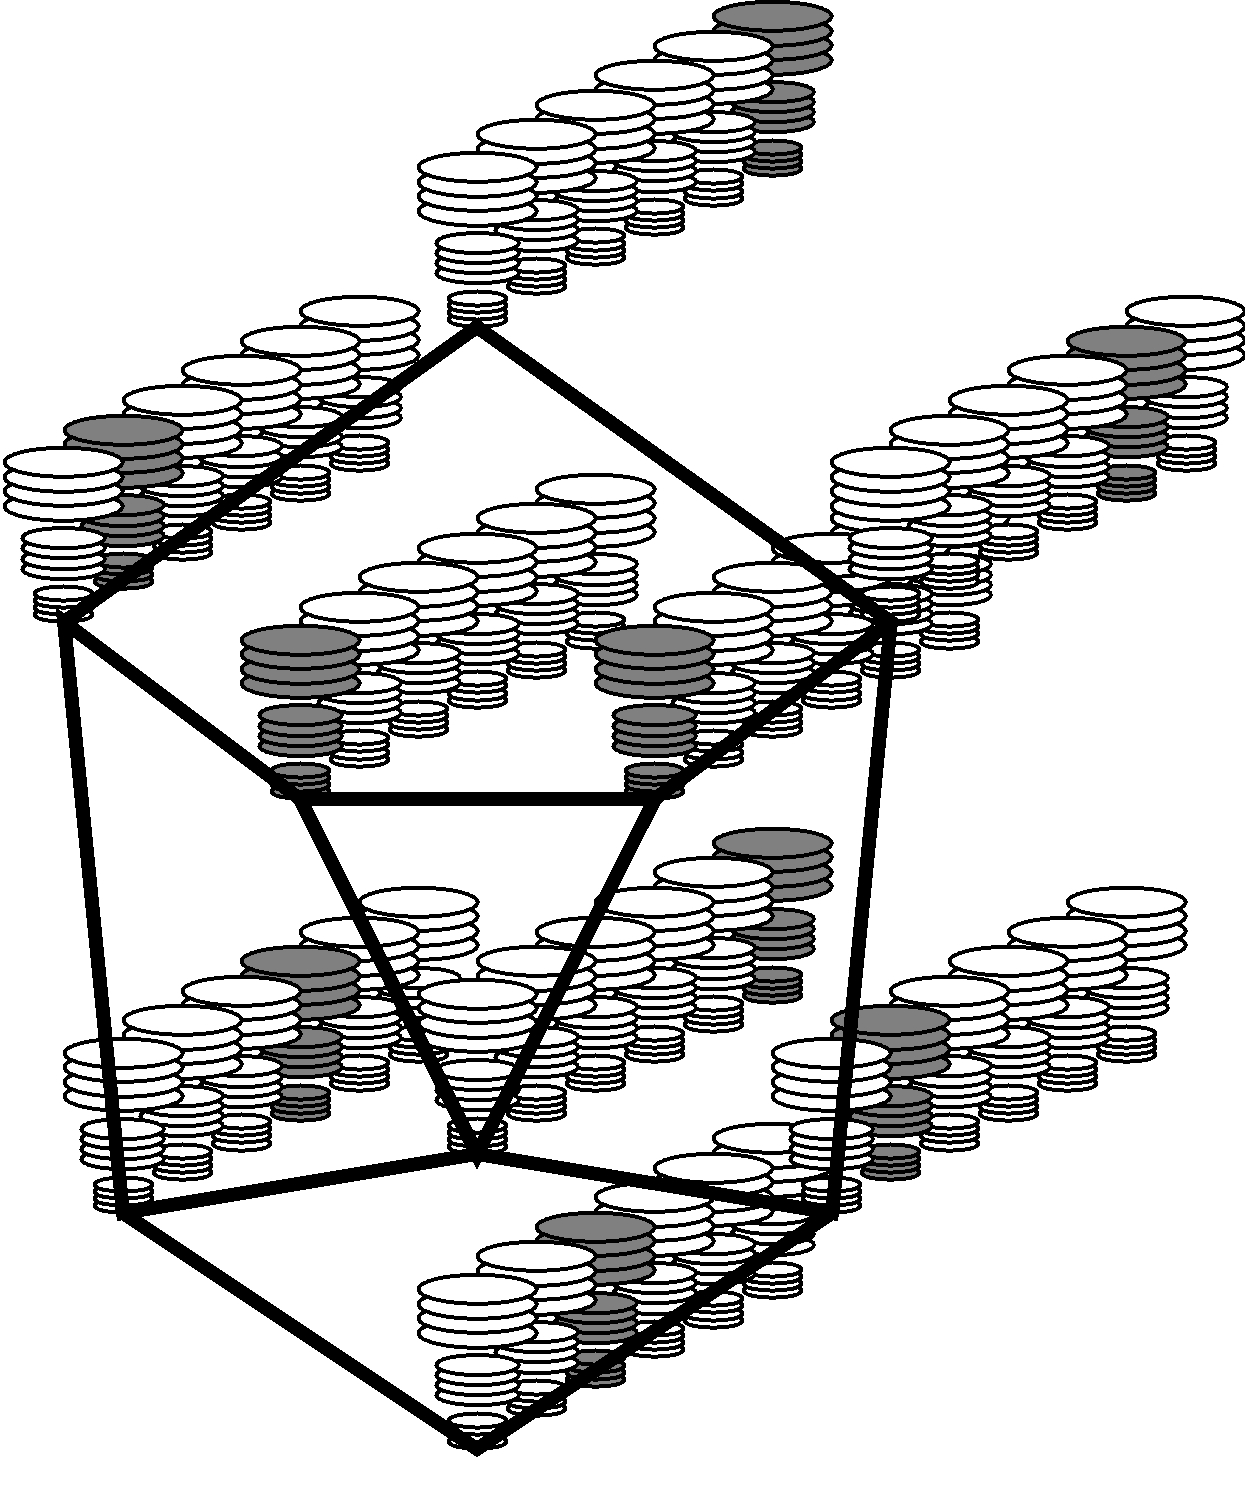
\includegraphics[scale=0.125]{ch2/figures/FBG.jpg}
  \caption{The Face Bunch Graph (FBG) serves as a general representation of faces. \cite{Wiskott1997}}
  \label{fig:FBG}
 \end{center}
\end{figure} 
Each model graph has the same structure. Nodes are referred to identical fiducial points called bunch. An eye bunch containing a set of jets, may represent closed, open, female and male eyes etc. 
\subsubsection{Graph Matching}
To represent a new face, the nodes are positioned on the face image by elastic bunch graph matching. A first set of graph is generated manually by locating fiducial points and connecting edges between them. Once an FBG is well defined, graphs for new images can be automatically generated by elastic bunch graph matching. Matching a FBG with a new image is done by maximising a graph similarity between an image graph and the FBG of identical pose. The graph similarity depends on the similarities of the jets and the topographic structure. Since the FBG provides several jets for every fiducial point, the best jet can be selected and reviewed. A heuristic algorithm is used to find the image which maximises the graph similarity function. The algorithm is as follows:
\begin{enumerate}
 \item The location of the face is found by a sparse scanning of the FBG over image.
 \item The size and position of face are refined. The FBG is varied in size and aspect ratio to adapt the right format of the face.
 \item All nodes are moved locally and relative to each other to optimise the graph similarity.
\end{enumerate}
The coarse to fine approach is applied so that the graph is extracted from the face image.
\subsubsection{Recognition}
After the graph has been generated from a new face image, the face is identified by comparing the similarity between an image graph and all model graphs. The graph with the highest similarity value is selected as the identity. The similarity function is an average over the similarities between pairs of corresponding jets. In \cite{Tefas2001}, the recognition of EBGM is enhanced by an approach using Support Vector Machine (SVM) which addresses the derivation of optimal coefficients. The coefficients measuring the local similarity values are determined by the elastic graph matching procedure at each grid node.

\subsection{Active Appearance Model}
An Active Appearance Model (AAM) is a statistical model generated by combining a model of shape variation with a model of texture variation. In the AAM, ``texture'' means the pattern of grey-level values (intensities) or colours across an image patch. The AAM successfully generalises almost every valid examples, but it brings optimisation difficulties on parameter selection. 
\subsubsection{Shape Models}
Building a shape model is based on a set of annotated face images. In these annotated face images, landmark points on faces are marked manually. These landmarks correspond to the key positions and outline of faces (as shown in \mbox{Figure} \ref{fig:labelled}). The shape is described in $n$ landmark points in 2-D images, so that the shape is represented by a vector $\mathbf{x}=(x_1,\ldots ,x_n,y_1,\ldots,y_n)^T$. In \cite{Edwards1998}, there are $400$ labelled face images , \textit{i.e.}, $400$ different shapes in the face image dataset. To align these shapes into a common coordinate frame, \textit{Procrustes analysis} \cite{Goodall1991} is used to minimise the sum of distances of each shape to the mean. Because the dimensionality of the shape vector $\mathbf{x}$ is high, PCA is used to reduce it into a more manageable manner. The shape vector $\mathbf{x}$ can be approximated through
\begin{equation}
 \mathbf{x} \approx \bar{\mathrm{x}} + \mathbf{\Phi} \mathbf{b}_s
\label{eq:APMPCA}
\end{equation}
where $\mathbf{\Phi}$ contains $t$ eigenvectors corresponding to the first $t$ largest eigenvalues, and $\bar{\mathrm{x}}$ is the mean shape. The vector $\mathbf{b}_s$ defines a set of $t$ parameters of a deformable model. Also \mbox{Equation} \ref{eq:APMPCA} can be formulated in a linear model
\begin{equation}
 \mathbf{x} =\bar{\mathrm{x}} + \mathbf{P}_s \mathbf{b}_s
\end{equation}
where $\mathbf{P}_s$ represents these $t$ eigenvectors, also called a set of orthogonal modes of shape variation. The number $t$ can be chosen so that the deformable model represents a $98\%$ proportion of the total variance of the data. A model of an image is described by the shape parameter $\mathbf{b}_s$, combined with a transformation from the coordinate frame. The parameters for the shape model is $(X_t,Y_t,s,\theta,\mathbf{b}_s)$ where $(X_t,Y_t)$ denotes the translation position, $s$ is the scaling factor, and $\theta$ is the rotation.
 \begin{figure}
  \begin{center}
   \subfigure[Labelled image]{\label{fig:labelled}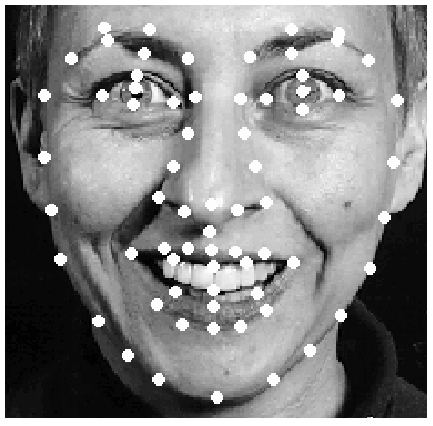
\includegraphics[scale=0.3]{ch2/figures/APMlabelledface.jpg}}
   \subfigure[Points]{\label{fig:points}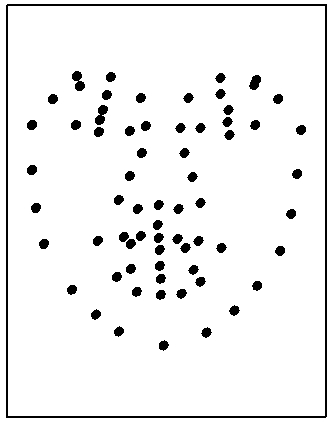
\includegraphics[scale=0.3]{ch2/figures/APMPoints.jpg}}
   \subfigure[Shape-free patch]{\label{fig:patch}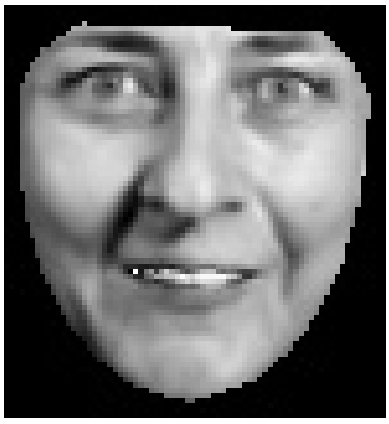
\includegraphics[scale=0.3]{ch2/figures/shapefreepatch.jpg}}
   \caption{A labelled training image gives a set of points and a shape-free patch.\cite{Cootes2001}}
  \end{center}
 \end{figure} 
\subsubsection{Appearance Models}
To build a texture model, \textit{triangulation algorithm} \cite{Cootes2000} is used to warp each example image. The control points on each image are matched against the mean shape model, so that a ``shape-free patch'' is obtained (shown in \mbox{Figure} \ref{fig:patch}). The shape-free patch is represented by a pixel-based grey-level vector $\mathbf{g}$. By applying PCA to the normalised patches generated from the training image set, a linear model is obtained as
\begin{equation}
 \mathbf{g} = \bar{\mathbf{g}} + \mathbf{P}_g \mathbf{b}_g
\end{equation}
where $\bar{\mathbf{g}}$ is the mean normalised grey-level vector, $\mathbf{P}_g$ is a set of orthogonal modes of grey-level variation, \textit{i.e.}, a set of eigenvectors, and $\mathbf{b}_g$ is a set of texture parameters.

The shape and texture of any example can be combined by the parameter vectors $\mathbf{b}_s$ and $\mathbf{b}_g$. The combined appearance model is
\begin{equation}
 \mathbf{b} = \left ( 
		\begin{array}{c}
		 \mathbf{W}_s \mathbf{b}_s \\
		 \mathbf{b}_g
		\end{array}
                   \right ) =
\left ( 
	\begin{array}{c}
	  \mathbf{W}_s \mathbf{P}_s^T(\mathbf{x}-\bar{\mathbf{x}}) \\
	  \mathbf{P}_g^T(\mathbf{g}-\bar{\mathbf{g}}) 
	\end{array}
\right )
\end{equation}
where $\mathbf{W}_s$ is a diagonal matrix of weights for each shape parameters. To explore correlations between the shape and texture variations, PCA is applied on the data, and gives a further model
\begin{equation}
 \mathbf{b} =  \mathbf{Q}  \mathbf{c}
\end{equation}
where $ \mathbf{Q}$ are the eigenvectors and $\mathbf{c}$ is a vector of appearance parameters controlling both the shape and texture of the model.

The appearance model is built on $400$ annotated face images \cite{Cootes1996}. On each annotated image, $122$ landmark points are on the key positions. A shape model is generated with $23$ parameters, and a shape-free grey-level model is generated with $114$ parameters from the $10000$-pixel patch. After the further PCA, the combined appearance model only contains $80$ parameters out of $114$, which cover $98\%$ of observed variation. \mbox{Figure} \ref{fig:AAMvariation} shows the effect of varying the first four appearance model parameters, showing changing in identity, pose and expression.
\begin{figure}[t]
 \begin{center}
  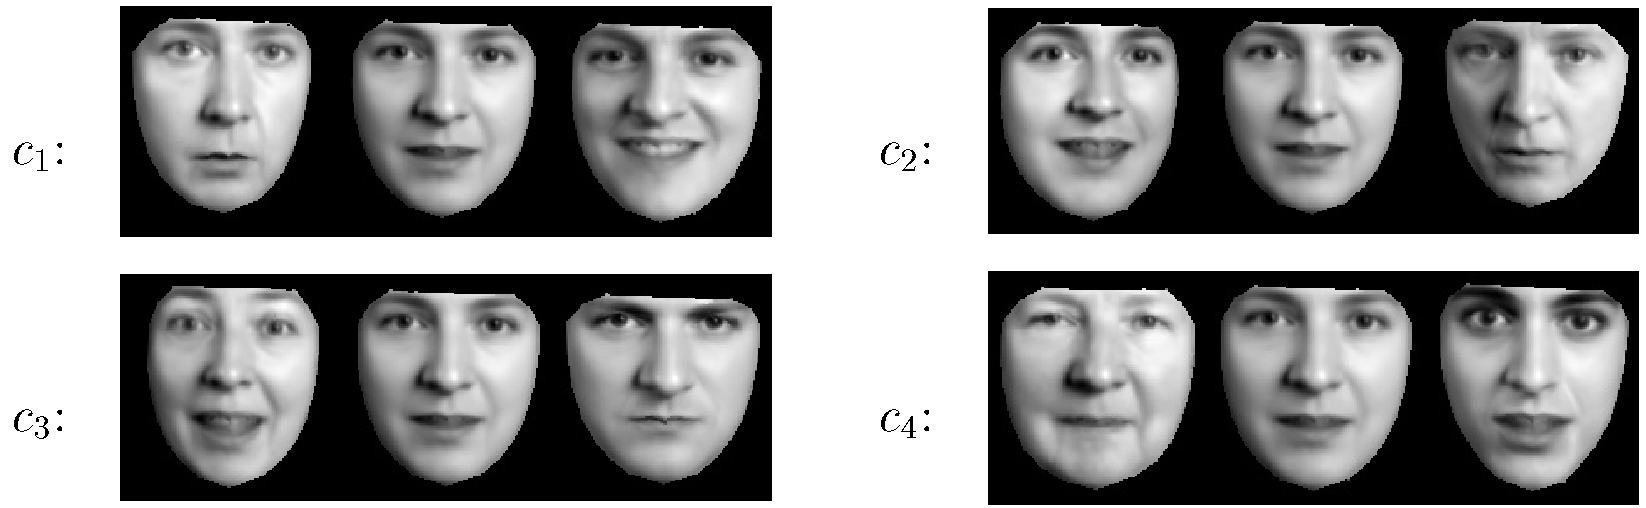
\includegraphics[width=\columnwidth]{ch2/figures/firstfourAAM.jpg}
  \caption{First four modes of appearance variation ($\pm 3$ sd) \cite{Cootes2001}}
  \label{fig:AAMvariation}
 \end{center}
\end{figure} 

\subsubsection{Model Matching}
Assuming a reasonable approximation, the model matching algorithm is to find the parameters of such a model which synthesises an image as close as to a target image. AAM matching is an optimisation problem in which the differences between a new image and a synthesised image by the appearance model is minimised. A different vector $\delta \mathbf{I}$ is defined as the subtracting between the gray-level values in the image and the gray-level values for the current model parameters. To find the best match between image and model, the magnitude of the difference vector $\Delta=|\delta \mathbf{I}|^2$ is minimised by varying with model parameters $\mathbf{c}$. The displacement of each model parameter from the correct value leads a special pattern in  $\delta \mathbf{I}$ and the error in the model parameters  $\delta \mathbf{c}$. In the training stage of AAM, a linear model is applied to learn the relationship between $\delta \mathbf{I}$ and $\delta \mathbf{c}$. In the matching stage of AAM, the knowledge of relationship is applied in an iterative algorithm for minimising $\Delta$. The iterative AAM matching is shown in \mbox{Figure} \ref{fig:AAMmatching}.
\begin{figure}[ht]
 \begin{center}
  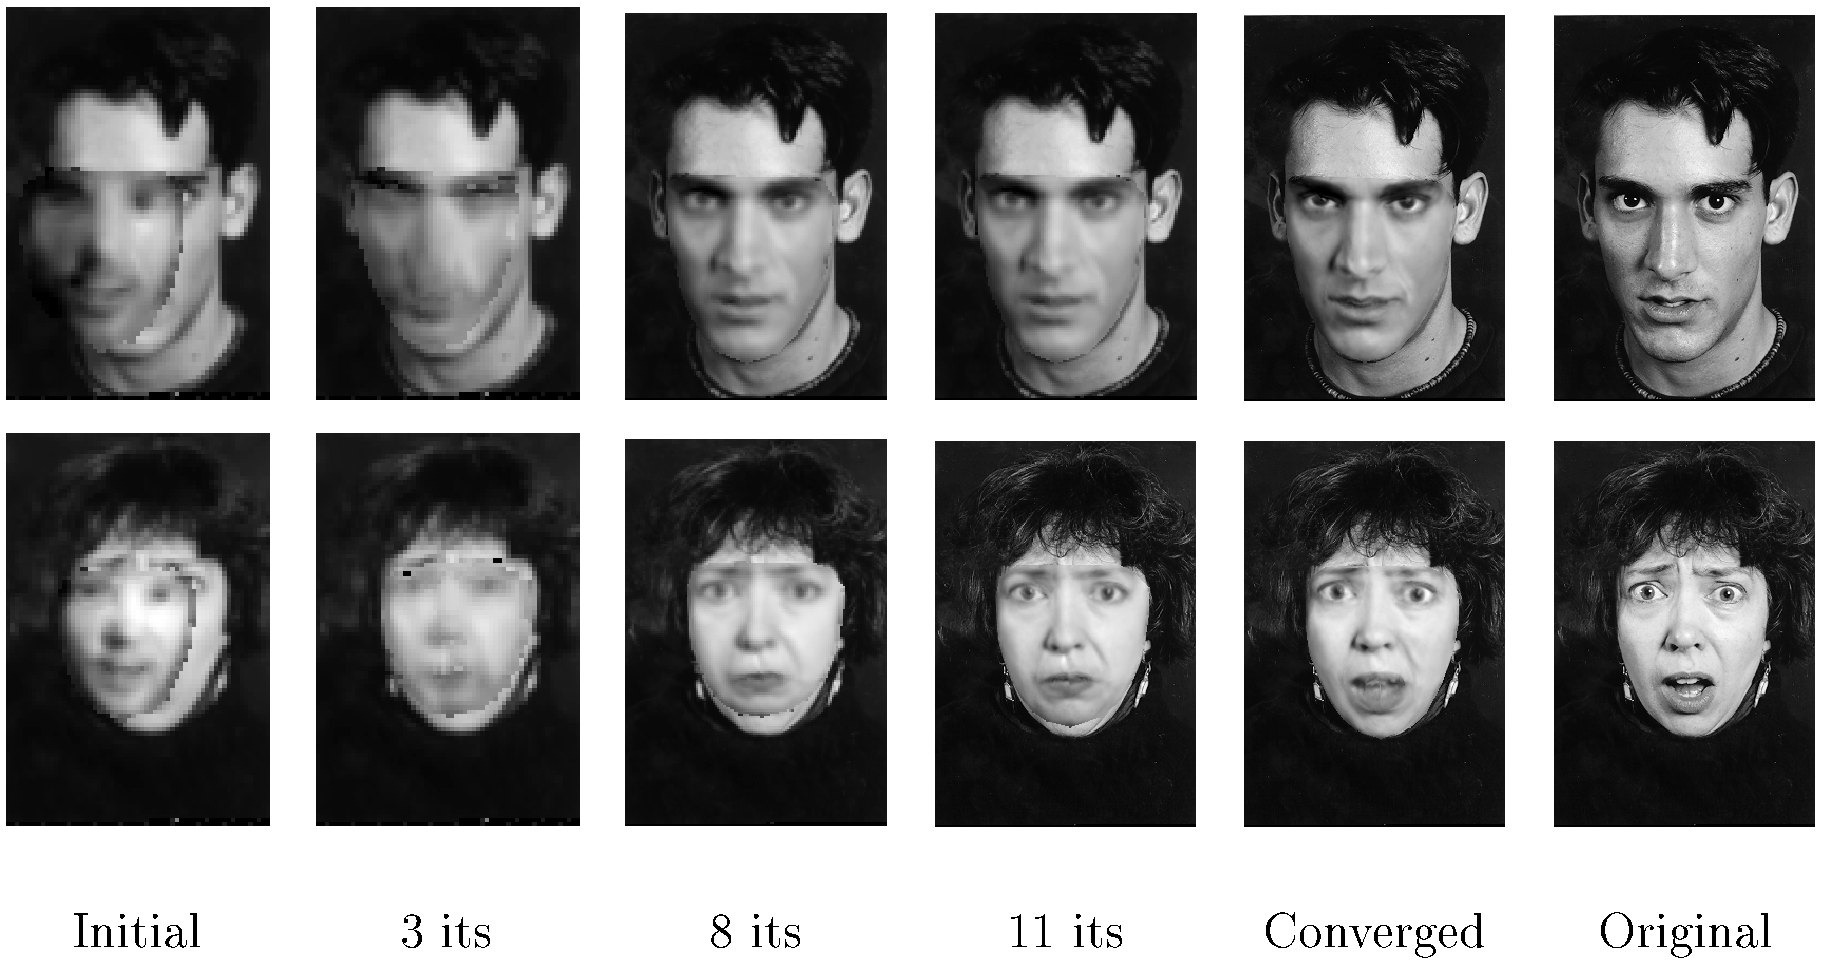
\includegraphics[width=\columnwidth]{ch2/figures/AAMmatching.jpg}
\caption{The two examples of the AAM matching iterations. \cite{Cootes2001}}
\label{fig:AAMmatching}
 \end{center}
\end{figure} 

\subsubsection{Recognition}
Once the appearance model has been matched to a new image, a full set of parameters can be computed. The classification system is used for recognising the individual appearing in an image. The classifier is trained by computing the appearance parameters for all training images (10 images for each of the 30 individuals \cite{Lanitis1997}), and establishing the distribution of appearance parameters for each individual. A discriminant analysis approach is used to enhance the effect of the inter-class variation. The metric is used as the Mahalanobis distance measure.

\subsection{Summary on model-based approaches}
The model-based approaches in face recognition exploit the intrinsic physical relationship with real faces. The physical relationship can be explained in geometric structure. Face variations due to different pose, illumination, and expression are modelled explicitly, which gives the possibility to handle these variations in practice. Prior knowledge on human faces is integrated into the approaches, so that not only statistic rules but also human knowledge are involved in face recognition. However, the model-based approaches suffer some drawbacks. 1) Constructing a model is very complicated and needs a lot of human intervention. Facial feature points are difficult to extract automatically with sufficient robustness. 2) Fitting or matching a model on an image is an optimisation process, which has highly computational costs since it is prone to be trapped into local minima. 3) The recognition results depend heavily on the results of fitting, so that there is a tradeoff between accuracy and computational cost in the fitting process. 4) For matching a model, a high resolution and high quality image is required. The model-based approaches also need complicated initialisation.

\section{3-D Morphable Face Model}\label{sec:3DMM}
The human faces can be treated as a manifold surface in a 3-D space. The 3-D morphable face model (3DMM) for face image synthesis and face recognition is developed by Blanz \textit{et al.} \cite{Blanz1999,Blanz2003}. One advantage of the 3-D morphable face model is that it can easily handle variation on pose and illumination instead of 2-D models, \textit{e.g.}, EBGM and AAM. The variance of pose and illumination is always obstacles for face recognition in 2-D space. Another advantage of the 3-D morphable face model is that a 3-D face surface is extracted from a single 2-D face image, which avoids expensive 3-D face/head scan. Face recognition uses the shape and texture parameters of the model, which represent intrinsic information of faces. 

\subsection{A Morphable Model of 3-D Faces}
In \cite{Blanz2003}, the morphable model is acquired from 3-D scans of 100 males and 100 females, aged between 18 and 45 years. These scans are recorded with a $Cyberwave$ 3030PS laser scanner. The scans represent face shape in cylindrical coordinates relative to a vertical axis centred as for the head. There are $512$ angular steps covering $360$ and $512$ vertical steps at a spacing of $0.615$mm. After the raw scans are obtained, some preprocessing is needed. 
\begin{enumerate}
 \item Holes are filled and spikes are removed on the face surface.
 \item 3-D data are aligned with a 3D-3D Absolute Orientation \cite{Haralick1992}.
 \item Heads are trimmed along the edge of a bathing cap.
 \item Heads are cut vertically behind the ears to remove the back of the head.
 \item Heads are cut horizontally at the neck to remove the shoulders.
\end{enumerate}
After above preprocessing, a modified optic flow method \cite{Horn1981,Bergen1990} is applied to establish dense point-to-point correspondence between a new face and a reference face. The shape and texture vectors of the reference face are
\begin{equation}
 \mathbf{S}_0 = (x_1,y_1,z_1,x_2,\ldots,x_n,y_n,z_n)^T
\end{equation}
\begin{equation}
 \mathbf{T}_0 = (R_1,G_1,B_1,R_2,\ldots,R_n,G_n,B_n)^T
\end{equation}
where the reference face is a triangular mesh with $75,972$ vertices ($n=75972$), $(x_k,y_k,z_k)$ is Cartesian coordinate for each vertex, and $(R_k,G_k,B_k)$ is the colour values from each vertex (and $k=1,\ldots,n$).

The PCA is performed on the set of shape and texture vectors $\mathbf{S}+i$ and $\mathbf{T}_i$ of $m$ example faces. There $m-1$ eigenvectors $\mathbf{s}_1,\mathbf{s}_2,\ldots$ are computed in the shape vectors from PCA by a Singular Value Decomposition (SVD) \cite{Press1992}. The eigenvectors construct an orthogonal basis on the shape vectors 
\begin{equation}
 \mathbf{S} = \bar{\mathbf{s}}+\sum_{i=1}^{m-1}\alpha_i\cdot \mathbf{s}_i
\end{equation}
where $\bar{\mathbf{s}}$ is the average from each shape vector, $\bar{\mathbf{s}}= \frac{1}{m}\sum_{i=1}^m \mathbf{S}_i$. So as to the texture vectors, an orthogonal basis is
\begin{equation}
 \mathbf{T} = \bar{\mathbf{t}}+\sum_{i=1}^{m-1}\beta_i\cdot \mathbf{t}_i
\end{equation}
The model coefficients $\alpha_i$ and $\beta_i$ are used to represent a face in an image.
\subsection{Morphable Model Fitting}
Face image synthesis defines the positions of vertices of the 3-D model with illumination and colour. During the processing of fitting a model with a novel image, not only the shape and texture parameters $\alpha_i$ and $\beta_i$ are optimised, but also the following rendering parameters are optimised. There are $22$ rendering parameters concatenated into a vector $\rho$: pose angles $\phi$, $\theta$, and $\gamma$, 3-D translation $\mathbf{t}_w$, focal length $f$, ambient lighting intensities $L_{r,amb},L_{g,amb},L_{b,amb}$, directed light intensities $L_{r,dir},L_{g,dir},L_{b,dir}$, the angles $\theta_l$ and $\phi_l$ of the directed light, colour contrast $c$, and gains and offsets of colour channels $g_r,g_g,g_b,o_r,o_g,o_b$. In analysis-by-synthesis iterations, the fitting algorithm finds model parameters and rendering parameters, and produces an image as similar as possible to the input image $\mathbf{I}_{input}$ as shown in \mbox{Figure} \ref{fig:modelvsinput}. 
\begin{figure}[t]
 \begin{center}
 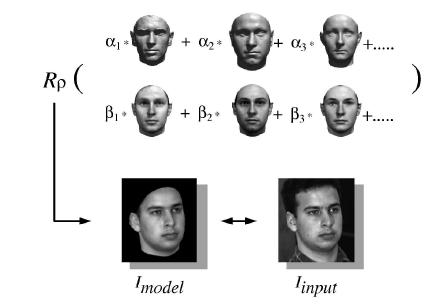
\includegraphics[width=0.77\columnwidth]{ch2/figures/3DMMfitting.jpg} 
 \caption{Fitting a morphable model: analysis by synthesis iterations.\cite{Blanz2003}}
  \label{fig:modelvsinput}
 \end{center}
\end{figure}
The goal of the fitting is to find shape and texture coefficients $\alpha$ and $\beta$ such that rendering $R_{\rho}$ produces an image $\mathbf{I}_{model}$ that is as similar as possible to $\mathbf{I}_{input}$.

The face reconstruction from a single image is shown in \mbox{Figure} \ref{fig:3DMMreconstruction}.
\begin{figure}[ht]
 \begin{center}
  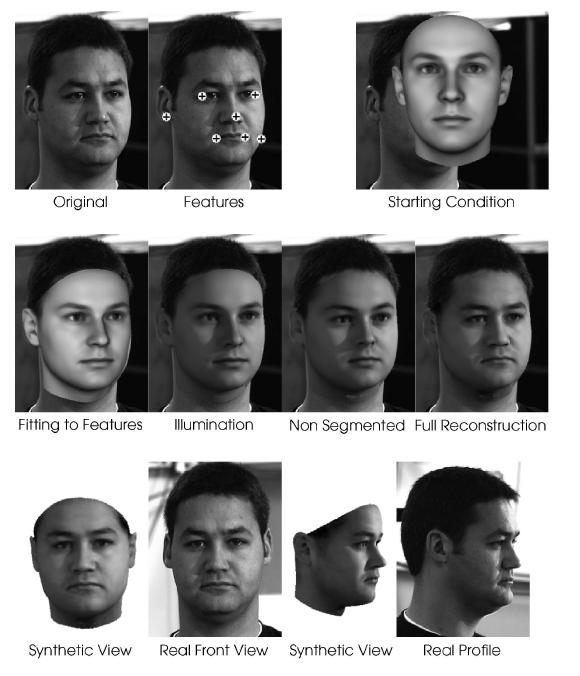
\includegraphics[width=0.77\columnwidth]{ch2/figures/3DMMreconstruction.jpg}
  \caption{The Face reconstruction from a single image by the 3-D morphable model. \cite{Blanz2003}}
  \label{fig:3DMMreconstruction}
 \end{center}
\end{figure}
For initialisation, seven facial feature points, such as the corner of the eyes or the tip of the nose, are marked in image coordinates. On the morphable model, these 7 points are also defined as vertices of the mesh corresponding to the points in the image.
The primary objective in analysing a face is to minimise the sum of square differences over all colour channels and all pixels in the input image and the symmetric reconstruction
\begin{equation}
 E_I = \sum_{x,y}\|  \mathbf{I}_{input}(x,y) -  \mathbf{I}_{model}(x,y) \|^2
\end{equation}
A stochastic version of Newton's method is used to minimise the cost function in the fitting procedure. Because the face model is separated into four regions - eyes, nose, mouth and the surrounding face area, the optimisation is also separated by each region to obtain local parameters, \textit{i.e.}, $\alpha_{r_1}, \beta_{r_1},\ldots,\alpha_{r_4}$ and $\beta_{r_4}$.

\subsection{Recognition}
After fitting the model, recognition can be performed based on model coefficients $\alpha$ and $\beta$, which represent intrinsic shape and texture information of faces. For identification, all gallery images are analysed by the fitting algorithm, and the shape and texture coefficients are stored. Given a probe (testing) image, the fitting algorithm computes coefficients which are compared with all images in the database to find the nearest neighbour. \mbox{Figure} \ref{fig:3DMMrecognition} shows the recognition scheme. Huang \textit{et al.} \cite{Huang2003} extended the 3-D morphable model with component-based recognition. Support Vector Machine (SVM) is used to decompose the face into a set of components. The system achieved $90\%$ recognition rate on a database of $1,200$ real images.
\begin{figure}[t]
 \begin{center}
  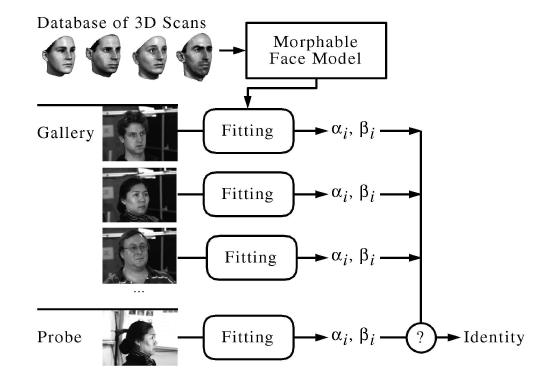
\includegraphics[width=0.77\columnwidth]{ch2/figures/3DMMrecognition.jpg}
  \caption{The recognition scheme in the 3-D morphable model. \cite{Blanz2003}}
  \label{fig:3DMMrecognition}
 \end{center}
\end{figure} 

\section{Other Approaches}
\label{sec:others}
There is a number of other approaches which have been explored in face recognition from different aspects. 
The \textit{trace transform} \cite{Kadyrov2001}, a generalisation of the radon transform, is a new tool for image processing which can be used for recognising faces \cite{Srisuk2003,Srisuk2003EE} under transformations, \textit{e.g.}, rotation, translation and scaling. Hidden Markov Model (HMM) \cite{Nefian1998} is an example of statistical model based approaches for face recognition. The pseudo two-dimensional HMM structure is proposed by Nefian and Hayes \cite{Nefian2000} for face detection and recognition.

\section{Face Database}\label{sec:facedatabase}
Along with the development of face recognition technology, a comparatively large number of face images in both training and testing sets have been collected. The face databases provide researchers a group of well-designed and organised face images, which are used for training and testing. In addition, with the numerous theories and techniques in face recognition, it is clear that evaluation and benchmarking of these algorithms is crucial. The face databases also provide a platform that evaluation could be done.

While there are many databases in use currently, the choice of an appropriate database to be used should be made based on the task given (aging, expressions, lighting etc). Another way is to choose the data set specific to the property to be tested (\textit{e.g.}, how algorithm behaves when given images with lighting changes or images with different facial expressions).

In this section, some face database popularly used by researchers are introduced. An comprehensive review on face databases on face detection, recognition and expression classification is conducted by Gross \cite{Gross2005}.

\subsubsection{Colour FERET}
The FERET \cite{Phillips1996} program set out to establish a large database of facial images that is gathered independently from the algorithm developers. The FERET database is collected in $15$ sessions between August 1993 and July 1996. The database contains $1,564$ sets of images for a total of $14,126$ images that includes $1,199$ individuals and $365$ duplicate sets of images.
A serial of FERET evaluations attract many institutions and companies to participate.
\subsubsection{XM2VTS}
The XM2VTS database \cite{Messer1999} contains four sessions of $295$ subjects taken over a period of four months. Each recording contains a speaking head shot and a rotating head shot. Sets of data taken from this database are available including high quality colour images, $32 KHz$ $16$-bit sound files, video sequences and a 3-D model.
\subsubsection{Yale}
The Yale face database \cite{Georghiades2001} contains $5,760$ single light source images of $10$ subjects each seen under $576$ viewing conditions ($9$ poses by $64$ illumination conditions). For every subject in a particular pose, an image with ambient (background) illumination was also captured.
\subsubsection{PIE}
The PIE database \cite{Sim2003} contains $41,368$ images of $68$ people, each person is under $13$ different poses, $43$ different illumination conditions, and with $4$ different expressions.
\subsubsection{ORL}
The ORL face database \cite{Samaria1994} contains ten different images of each of $40$ distinct subjects. For some subjects, the images were taken at different times, varying the lighting, facial expressions (open or closed eyes, smiling or not smiling) and facial details (glasses or no glasses). All the images were taken against a dark homogeneous background with the subjects in an upright, frontal position (with tolerance for some side movement).
\subsubsection{MIT-CBCL}
The MIT-CBCL face recognition database \cite{Weyrauch2004} contains face images of $10$ subjects. It provides two training sets. The first training set contains high resolution pictures, including frontal, half-profile and profile view. The second training set are synthetic images ($324$ per subject) rendered from 3-D head models of the $10$ subjects. The head models are generated by fitting a morphable model to the high-resolution training images, but the 3-D model is not included in the database. The testing set consists of $200$ images per subject. 
\subsubsection{AR Face Database}
The AR face database \cite{Martinez1998} contains $4,000$ colour images corresponding to $126$ individuals ($70$ men and $56$ women). Images feature frontal view faces with different facial expressions, illumination conditions, and occlusions (sun glasses and scarf).
%\subsubsection{BioID}
%The BioID dataset \cite{Jesorsky2001} consists of $1521$ gray level images with a resolution of $384\times 286$ pixel. Each one shows the frontal view of a face out of $23$ different test persons. For comparison reasons the dataset also contains manually set eye postions.
\subsubsection{UMIST Face Database}
The UMIST face database \cite{Graham1998} consists of $564$ images of $20$ people. Each covering a range of poses from profile to frontal views. Subjects cover a range of race, sex, and appearance. Each subject exists in their own directory labelled and images are numbered consequently as they were taken. The files are all in PGM format, approximately $220 \times 220$ pixels in $256$ shades of grey.
\section{Summary}
In this chapter, an extensive review on face recognition is conducted. Two types of state-of-the-art approaches for face recognition are introduced. A 2-D combined with 3-D approach is also reviewed. Face recognition is still a very challenging topic after 30 years of research \cite{Zhao2003}. Pose and illuminance are still two major problems that degrade the performance of face recognition systems. Appearance-based approaches focus on statistical distribution of facial texture. The texture is locally distributed on human faces. Also, appearance-based approaches abandon some prior information of human faces, \textit{e.g.}, head, hair, ears and so on. Model-based approaches focus on the topologyl and shapes of faces, but ignore the statistical analysis of facial texture. It proves that appearance-based and model-based approaches can be combined, such that appearance-based approaches deal with local texture information, and model-based approaches deal with global shape information.



\chapter{Gabor Wavelet and AdaBoost}
\label{ch:gaboradaboost}
This chapter presents the fundamentals of the Gabor-Boosting algorithm: Gabor wavelets and AdaBoost. \mbox{Section} \ref{sec:faceveri} discusses the Gabor wavelets and how face images are represented by Gabor wavelet features. In \mbox{Section} \ref{sec:faceveri:adaboost}, the AdaBoost algorithm is presented, and the principle of constructing the ``strong'' AdaBoost ensemble classifier, is discussed.
\section{Gabor Wavelets}
\label{sec:faceveri}
A 2-D Gabor filter is a linear filter whose kernel is similar to the 2-D receptive profiles of the mammalian cortical simple cells \cite{Jones1987}. A 2-D Gabor kernel is a 2-D Gaussian function multiplied by a 2-D harmonic function. Generally, a harmonic function is a Fourier basis function. Especially, in a 2-D Gabor kernel it is a sinusoidally modulated function, in a form of complex exponential function. The Gaussian function varies in dilation and the harmonic function varies in rotation and frequency, so that a group of 2-D Gabor filters can be formed into 2-D Gabor wavelets. Gabor wavelets capture local structure corresponding to spatial frequency, \textit{i.e.}, scale, spatial localisation (coordinates), and orientation selectivity.

Gabor wavelets are used to extract facial information from face images. \mbox{Section} \ref{sec:backgoundGabor} gives the background study on Gabor wavelets. The definition of Gabor wavelet is given in \mbox{Section} \ref{sec:definGabor}. \mbox{Section} \ref{sec:gaborwavelettransform} illustrates the Gabor wavelet transform. \mbox{Section} \ref{sec:gaborwaveletfeature} presents the representatives of face images - Gabor wavelet features.
\subsection{Background of Gabor Wavelets}
\label{sec:backgoundGabor}
2-D Gabor wavelets are widely adopted as a feature extraction approach in texture segmentation \cite{Dunn1994,Dunn1995,Jain1991,Teuner1995}, iris recognition \cite{Daugman1988}, face recognition \cite{Wiskott1997,Wiskott1999}, face expression recognition \cite{Hong1998,Lyons1999,Zhang1998}, and image retrieval \cite{Manjunath1996}.

When Gabor filters are applied on computer vision or image processing tasks, the one biggest problem is how to select the appropriate Gabor filters, \textit{i.e.}, finding appropriate parameters for Gabor filters. The parametric characterisation has been studied extensively and different types of schemes have emerged. In \cite{Dunn1994}, 2-D Gabor filters transform different texture into detectable filter-output discontinuities at texture boundaries. Gabor filter output is modeled as Rician random variables \cite{Dunn1994}. A decision algorithm for selecting optimal filter parameters based on the Rician model is developed by Dunn and Higgins \cite{Dunn1995}. In \cite{Jain1991}, a bank of Gabor filters is characterised as uniformly covering the spatial-frequency domain, and a filter selection scheme is presented based on minimal ``energy'' loss in reconstructed images from the filtered images. Teuner \textit{et al.} \cite{Teuner1995} choose parameters of Gabor filters based on the analysis of spectral feature contrasts obtained from iterations of pyramidal Gabor transforms. The work benefit from not needing prior knowledge of the texture image which means the segmentation processing is unsupervised. Since these parametrization solutions are all to choose optimal frequency or orientation of Gabor filter, an alternative wavelet scenario is proposed to bypass the optimisation. 

A 2-D Gabor wavelet model with multi-scale and multi-orientation is originally proposed by Daugman \cite{Daugman1985, Daugman1988} for biometric research. In \cite{Daugman1988}, by using a three-lay neural network, a nonorthogonal 2-D Gabor representation is generalised. Daugman also has applied his 2-D Gabor wavelet model on human iris recognition.  In \cite{Daugman1993}, the visible texture of the human iris is transformed as a sequence of multi-scale 2-D Gabor wavelet digits. Lades \textit{et al.} \cite{Lades1993} has applied Gabor wavelets for face recognition using the Dynamic Link Architecture (DLA) framework. The DLA starts by computing Gabor wavelets, and then it performs a flexible template comparison between resulting image decompositions using graph-matching. Wiskott \textit{et al.} \cite{Wiskott1997,Wiskott1999} have extended on DLA by developing a Gabor wavelet based Elastic Bunch Graph Matching (EBGM) to label and recognise faces. Faces are represented by labelled graphs using Gabor wavelet transform. The labelled graphs consist of nodes and edges which are positioned by elastic bunch graph matching processing for comparing similarities. The testing is done on the FERET database \cite{Phillips2000} showing a high recognition rate for frontal face images. Liu and Wechsler \cite{Liu2002} applied the Enhanced Fisher linear discriminant Model (EFM) to an augmented Gabor feature vector \cite{Liu2001} derived from the Gabor wavelet representation of face images. Liu \cite{Liu2004} also presents a Gabor-based kernel Principal Component Analysis (PCA) method by integrating Gabor wavelet representation and the kernel PCA for recognition.  Fan \textit{et al.} \cite{Fan2004} combined Gabor wavelet and Null space-based Linear Discriminate Analysis (LDA) simultaneously on each orientations for generating feature vectors.

In analysis of facial expression, the recognition is to analyse the relationship between the movements made by facial features, such as eyebrows, eyes and mouth. These facial features can be defined as point-based visual properties of facial expressions. Hong \textit{et al.} \cite{Hong1998} use Gabor wavelets of five frequencies and eight orientations to define a ``big'' General Face Knowledge (GFK) with $50$ nodes\footnote{The nodes are landmark points on human faces.} on a face, and a ``small'' $16$-node GFK with three frequencies and four orientations. The method which fits these nodes with face image is the elastic graph matching proposed by Wiskott \textit{et al.} \cite{Wiskott1997,Wiskott1999} in face recognition. Zhang \textit{et al.} \cite{Zhang1998} use $34$ facial points for which a set of Gabor wavelet coefficients, the Gabor wavelets with three frequencies and six orientations have been utilised. Lyons \textit{et al.} \cite{Lyons1999} use a fiducial grid of $34$ nodes and apply wavelets of five frequencies and six orientations.


\subsection{The Definition of Gabor Wavelets}
\label{sec:definGabor}
Gabor wavelets are introduced to image analysis due to their biological relevance and computational properties \cite{Jones1987}. A Gabor wavelet \cite{Daugman1988} (sometimes, called Gabor Kernel or Gabor Elemental Function \cite{Dunn1994}) is defined as 
\begin{equation}\label{eq:kernel}
\psi_{\mu,\nu}(z)=\frac{\|{k_{\mu,\nu}}\| ^ {2}}{\sigma ^{2}}e^{-\frac{\|{k_{\mu,\nu}}\|^ {2}\|z\|^{2}}{2\sigma ^{2}}}\lbrack{e^{ik_{\mu,\nu} z}-e^{-\frac{\sigma^2}{2}}}\rbrack
\end{equation}
where $z=(x,y)$ indicates a point with $x$, the horizontal coordinate and $y$, the vertical coordinate. The parameters $\mu$ and $\nu$ define the angular orientation and the spatial frequency of the Gabor kernel. In \mbox{Equation} \ref{eq:kernel}, the spatial frequency modulates the size of the 2-D discrete Gabor kernel, so that $\nu$ also determines the scale of kernel. The operator $\|\cdot\|$ denotes the norm operator. The parameter $\sigma$ is the standard deviation of Gaussian window in the kernel. The wave vector $k_{\mu,\nu}$ is defined as
\begin{equation}\label{eq:wavevector}
k_{\mu,\nu}=k_{\nu}e^{i\phi_{\mu}}
\end{equation}
where $k_{\nu}=\frac{k_{max}}{f^{\nu}}$ and $\phi_{\mu}=\frac{\pi\mu}{8}$ if eight different orientations have been chosen. $k_{max}$ is the maximum frequency, and $f$ is the spatial factor between
kernels in the frequency domain.
\subsubsection{Wavelets}
Gabor kernels in \mbox{Equation} (\ref{eq:kernel}) are all self-similar since they are generated from one kernel (from one mother wavelet) by dilation and rotation via the wave vector $k_{\mu,\nu}$. Each kernel is a product of a Gaussian envelope formulated in the \mbox{Equation}
\begin{equation}\label{eq:gaussian}
 \frac{\|{k_{\mu,\nu}}\| ^ {2}}{\sigma ^{2}}e^{-\frac{\|{k_{\mu,\nu}}\|^ {2}\|z\|^{2}}{2\sigma ^{2}}}\
\end{equation}
and a complex plane wave $e^{ik_{\mu,\nu} z}$. The complex wave determines the oscillatory part of the kernel. The term $-e^{-\frac{\sigma^2}{2}}$ compensates for the Disparity Compensated (DC) value which makes the kernel DC-free. DC-free \cite{Krueger2001} is a wavelet terminology that ensures wavelets do not lose any generality such that there is no minimal energy loss when images are reconstructed by the wavelets. The effect of the DC term becomes negligible when the parameter $\sigma$, which determines the ratio of the Gaussian window width to wavelength, is a sufficiently large value.

\subsubsection{Parametrization}
In this thesis, five different scales and eight orientations of Gabor wavelets are used, i.e., $\nu\in\{-1,\ldots,3\}$, and $\mu\in\{0,\ldots,7\}$. Since images used in this thesis are smaller than the images with $128\times 128$ size used in \cite{Wiskott1997,Wiskott1999}, the scale range is from $-1$ to $3$ rather than from $0$ to $4$. The eight orientations in radian are from $0$ to $7\pi/8$ with a $\pi/8$ interval. Gabor wavelets are modulated by a Gaussian envelope function with relative width $\sigma=2\pi$. The maximum frequency is $k_{max}=\frac{\pi}{2}$, and the factor $f=\sqrt{2}$. These parameters are chosen according to previous findings \cite{Wiskott1999,Liu2004}. The kernels exhibit desirable characteristics of spatial frequency, spatial locality, and orientation selectivity. 

\subsubsection{Complex Gabor}
Gabor kernel is a product of a Gaussian and a complex plane wave with real and imaginary parts, also called even and odd. The \mbox{Equation} \ref{eq:kernel} is separated into real and imaginary parts, so that the real part is
\begin{equation}\label{eq:real}
\frac{k_{\nu}^2}{\sigma^2}e^{-{\frac{\|z\|^2 k_{\nu}^2}{2\sigma^2}}} \{\cos(k_{\nu}\cos(\phi_{\mu})x+k_{\nu}\sin(\phi_{\mu})y)-e^-{\frac{\sigma^2}{2}}\}
\end{equation}
and the imaginary part becomes
\begin{equation}\label{eq:imag}
\frac{k_{\nu}^2}{\sigma^2} e^-{\frac{\|z\|^2 k_{\nu}^2}{2\sigma^2}} \sin(k_{\nu}\cos(\phi_{\mu})x+k_{\nu}\sin(\phi_{\mu})y)
\end{equation}
The real part and the imaginary part of $40$ Gabor wavelets are shown in \mbox{Figure} \ref{fig:realgabor} and \mbox{Figure} \ref{fig:imaggabor} respectively.
\begin{figure}[ht]
 \begin{center}
 
\includegraphics[width=\columnwidth/9]{ch4/figures/rGabor0_0.jpg}
 
\includegraphics[width=\columnwidth/9]{ch4/figures/rGabor0_1.jpg}
 
\includegraphics[width=\columnwidth/9]{ch4/figures/rGabor0_2.jpg}
 
\includegraphics[width=\columnwidth/9]{ch4/figures/rGabor0_3.jpg}
 
\includegraphics[width=\columnwidth/9]{ch4/figures/rGabor0_4.jpg}
 
\includegraphics[width=\columnwidth/9]{ch4/figures/rGabor0_5.jpg}
 
\includegraphics[width=\columnwidth/9]{ch4/figures/rGabor0_6.jpg}
 
\includegraphics[width=\columnwidth/9]{ch4/figures/rGabor0_7.jpg}\\
 
\includegraphics[width=\columnwidth/9]{ch4/figures/rGabor1_0.jpg}
 
\includegraphics[width=\columnwidth/9]{ch4/figures/rGabor1_1.jpg}
 
\includegraphics[width=\columnwidth/9]{ch4/figures/rGabor1_2.jpg}
 
\includegraphics[width=\columnwidth/9]{ch4/figures/rGabor1_3.jpg}
 
\includegraphics[width=\columnwidth/9]{ch4/figures/rGabor1_4.jpg}
 
\includegraphics[width=\columnwidth/9]{ch4/figures/rGabor1_5.jpg}
 
\includegraphics[width=\columnwidth/9]{ch4/figures/rGabor1_6.jpg}
 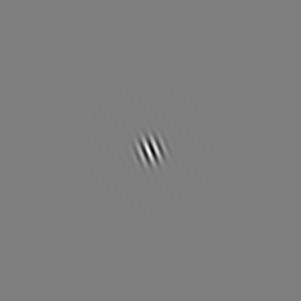
\includegraphics[width=\columnwidth/9]{ch4/figures/rGabor1_7.jpg}\\
 
\includegraphics[width=\columnwidth/9]{ch4/figures/rGabor2_0.jpg}
 
\includegraphics[width=\columnwidth/9]{ch4/figures/rGabor2_1.jpg}
 
\includegraphics[width=\columnwidth/9]{ch4/figures/rGabor2_2.jpg}
 
\includegraphics[width=\columnwidth/9]{ch4/figures/rGabor2_3.jpg}
 
\includegraphics[width=\columnwidth/9]{ch4/figures/rGabor2_4.jpg}
 
\includegraphics[width=\columnwidth/9]{ch4/figures/rGabor2_5.jpg}
 
\includegraphics[width=\columnwidth/9]{ch4/figures/rGabor2_6.jpg}
 \includegraphics[width=\columnwidth/9]{ch4/figures/rGabor2_7.jpg}\\
 \includegraphics[width=\columnwidth/9]{ch4/figures/rGabor3_0.jpg}
 \includegraphics[width=\columnwidth/9]{ch4/figures/rGabor3_1.jpg}
 \includegraphics[width=\columnwidth/9]{ch4/figures/rGabor3_2.jpg}
 \includegraphics[width=\columnwidth/9]{ch4/figures/rGabor3_3.jpg}
 \includegraphics[width=\columnwidth/9]{ch4/figures/rGabor3_4.jpg}
 \includegraphics[width=\columnwidth/9]{ch4/figures/rGabor3_5.jpg}
 \includegraphics[width=\columnwidth/9]{ch4/figures/rGabor3_6.jpg}
 \includegraphics[width=\columnwidth/9]{ch4/figures/rGabor3_7.jpg}\\
 \includegraphics[width=\columnwidth/9]{ch4/figures/rGabor4_0.jpg}
 \includegraphics[width=\columnwidth/9]{ch4/figures/rGabor4_1.jpg}
 \includegraphics[width=\columnwidth/9]{ch4/figures/rGabor4_2.jpg}
 \includegraphics[width=\columnwidth/9]{ch4/figures/rGabor4_3.jpg}
 \includegraphics[width=\columnwidth/9]{ch4/figures/rGabor4_4.jpg}
 \includegraphics[width=\columnwidth/9]{ch4/figures/rGabor4_5.jpg}
 \includegraphics[width=\columnwidth/9]{ch4/figures/rGabor4_6.jpg}
 \includegraphics[width=\columnwidth/9]{ch4/figures/rGabor4_7.jpg}\\
\caption{The real part of the $5\times8$ Gabor wavelets.}
\label{fig:realgabor}
\end{center}
\end{figure} 
\begin{figure}[ht]
 \begin{center}
 \includegraphics[width=\columnwidth/9]{ch4/figures/iGabor0_0.jpg}
 \includegraphics[width=\columnwidth/9]{ch4/figures/iGabor0_1.jpg}
 \includegraphics[width=\columnwidth/9]{ch4/figures/iGabor0_2.jpg}
 \includegraphics[width=\columnwidth/9]{ch4/figures/iGabor0_3.jpg}
 \includegraphics[width=\columnwidth/9]{ch4/figures/iGabor0_4.jpg}
 \includegraphics[width=\columnwidth/9]{ch4/figures/iGabor0_5.jpg}
 \includegraphics[width=\columnwidth/9]{ch4/figures/iGabor0_6.jpg}
 \includegraphics[width=\columnwidth/9]{ch4/figures/iGabor0_7.jpg}\\
 \includegraphics[width=\columnwidth/9]{ch4/figures/iGabor1_0.jpg}
 \includegraphics[width=\columnwidth/9]{ch4/figures/iGabor1_1.jpg}
 \includegraphics[width=\columnwidth/9]{ch4/figures/iGabor1_2.jpg}
 \includegraphics[width=\columnwidth/9]{ch4/figures/iGabor1_3.jpg}
 \includegraphics[width=\columnwidth/9]{ch4/figures/iGabor1_4.jpg}
 \includegraphics[width=\columnwidth/9]{ch4/figures/iGabor1_5.jpg}
 \includegraphics[width=\columnwidth/9]{ch4/figures/iGabor1_6.jpg}
 \includegraphics[width=\columnwidth/9]{ch4/figures/iGabor1_7.jpg}\\
 \includegraphics[width=\columnwidth/9]{ch4/figures/iGabor2_0.jpg}
 \includegraphics[width=\columnwidth/9]{ch4/figures/iGabor2_1.jpg}
 \includegraphics[width=\columnwidth/9]{ch4/figures/iGabor2_2.jpg}
 \includegraphics[width=\columnwidth/9]{ch4/figures/iGabor2_3.jpg}
 \includegraphics[width=\columnwidth/9]{ch4/figures/iGabor2_4.jpg}
 \includegraphics[width=\columnwidth/9]{ch4/figures/iGabor2_5.jpg}
 \includegraphics[width=\columnwidth/9]{ch4/figures/iGabor2_6.jpg}
 \includegraphics[width=\columnwidth/9]{ch4/figures/iGabor2_7.jpg}\\
 \includegraphics[width=\columnwidth/9]{ch4/figures/iGabor3_0.jpg}
 \includegraphics[width=\columnwidth/9]{ch4/figures/iGabor3_1.jpg}
 \includegraphics[width=\columnwidth/9]{ch4/figures/iGabor3_2.jpg}
 \includegraphics[width=\columnwidth/9]{ch4/figures/iGabor3_3.jpg}
 \includegraphics[width=\columnwidth/9]{ch4/figures/iGabor3_4.jpg}
 \includegraphics[width=\columnwidth/9]{ch4/figures/iGabor3_5.jpg}
 \includegraphics[width=\columnwidth/9]{ch4/figures/iGabor3_6.jpg}
 \includegraphics[width=\columnwidth/9]{ch4/figures/iGabor3_7.jpg}\\
 \includegraphics[width=\columnwidth/9]{ch4/figures/iGabor4_0.jpg}
 \includegraphics[width=\columnwidth/9]{ch4/figures/iGabor4_1.jpg}
 \includegraphics[width=\columnwidth/9]{ch4/figures/iGabor4_2.jpg}
 \includegraphics[width=\columnwidth/9]{ch4/figures/iGabor4_3.jpg}
 \includegraphics[width=\columnwidth/9]{ch4/figures/iGabor4_4.jpg}
 \includegraphics[width=\columnwidth/9]{ch4/figures/iGabor4_5.jpg}
 \includegraphics[width=\columnwidth/9]{ch4/figures/iGabor4_6.jpg}
 \includegraphics[width=\columnwidth/9]{ch4/figures/iGabor4_7.jpg}\\
\caption{The imaginary part of the $5\times8$ Gabor wavelets.}
\label{fig:imaggabor}
\end{center}
\end{figure} 
These Gabor wavelets share 5 scales and 8 orientations. The orientations from left to right are $0,\frac{\pi}{8},\frac{\pi}{4},\frac{3\pi}{8},\frac{\pi}{2},\frac{5\pi}{8},\frac{3\pi}{4},$ and $\frac{7\pi}{8}$. The scales from top to bottom are $-1$, $0$, $1$, $2$, $3$.

\subsection{Gabor Wavelet Transform}
\label{sec:gaborwavelettransform}
In computer vision, \textit{features} stand as a piece of ``interesting'' information which is relevant for solving a specific vision application. In appearance based approaches, features refer to the result after a general neighbourhood operation applied on an image. The result contains local or global information which contributes to resolving a specific vision problem. An image can be represented by a group of features. A computer vision system works on these features rather than image pixels directly.
Extraction of features is defined in terms of local neighbourhood operations. In this thesis, Gabor wavelet transform is the process to extract features which are relevant to face recognition. Since the selective schemes are available with a range of frequencies and orientation intervals, Gabor wavelets are ideal for face feature representation.

This section illustrates the Gabor wavelet transform by convolution. First of all, the concept of convolution is given. Secondly, the 2-D discrete convolution is presented. Thirdly, the size of mask for convolution is determined. Finally, the magnitude response is used as extracted features.
\subsubsection{Convolution}
The Gabor wavelet transform is the course of two-dimensional convolution of an image with a family of Gabor wavelet kernels defined by \mbox{Equation} \ref{eq:kernel}. Two-dimensional (2-D) convolution \cite{Sonka1998} is a specific type of local neighbourhood operation which belongs to the linear approach in image analysis. The 2-D convolution $g$ of two-dimensional functions $f$ and $h$ is denoted by $f*h$. The function of 2-D convolution is expressed as
\newcommand{\ud}{\mathrm{d}}
{\setlength\arraycolsep{2pt}
\begin{eqnarray}\label{eq:conv2}
 g(x, y) = \int_{-\infty}^{\infty}\int_{-\infty}^{\infty}f(a,b)h(x-a,y-b) \, \ud a \, \ud b \nonumber\\
= \int_{-\infty}^{\infty}\int_{-\infty}^{\infty}f(x-a,y-b)h(a,b) \, \ud a \, \ud b \nonumber\\
= (f*h)(x,y) = (h*f)(x,y) ��\end{eqnarray}
} 
where the operator $*$ symbolise the convolution operator. The 2-D convolution is an integral of the functions $f$ and $h$. The convolution means a linear filtering process using the filter $h$ on the image $f$.  The linear filtering is often used in local image pre-processing.

\subsubsection{2-D discrete convolution}
In the 2-D discrete image domain, the linear filtering calculates the image pixel $g(x,y)$ as a linear combination of the pixel value in a local neighbourhood of the pixel $f(a,b)$. The 2-D discrete convolution is described as
\begin{equation}
 %g(x,y)=\sum^{\infty}_{a=-\infty}\sum^{\infty}_{b=-\infty}f(a,b)h(x-a,y-b)
g(x,y)=\sum_{a}\sum_{b}f(a,b)h(x-a,y-b)
\end{equation}
where $f(a,b)$ is the 2-D discrete input image and $h(x,y)$ is the so-called \textbf{convolution mask} or convolution kernel. The convolution mask is often used with an odd number of pixels in rows and columns, such as $3\times3$, $5\times5$ and so on. An example \cite{Davies1990} of a $3\times3$ convolution mask is
\begin{displaymath}
 \left[  \begin{array}{ccc}
          \mathrm{h}_{4} &\mathrm{h}_{3} & \mathrm{h}_{2} \\
	  \mathrm{h}_{5} & \mathrm{h}_{0} & \mathrm{h}_{1} \\
	  \mathrm{h}_{6} & \mathrm{h}_{7} & \mathrm{h}_{8} 
         \end{array}
\right ]
\end{displaymath}
where $\mathrm{h}_{n}$ is the coefficient of the convolution mask. The 2-D convolution result is the linear neighbourhood operation weighted by the corresponding coefficients in the mask $h$. In practice, fast convolution is used to increase the speed of the convolution. A fast convolution algorithm takes the fast Fourier transform (FFT) of the input image and the convolution mask, multiplies them together, and then performs the inverse fast Fourier transform (IFFT). In this thesis, the 2-D discrete convolution function is provided by OpenCV \cite{Landre2003} in implementation.
\subsubsection{The Size of Mask}
In 2-D discrete convolution, the size of a Gabor filtering convolution mask is an important issue. It should be large enough to show the nature of Gabor wavelets. However, it should not be too large, otherwise computation cost will be increased. For instance, in \mbox{Figure} \ref{fig:realgabor}, the size of the Gabor convolution masks is $301\times301$, and the Gabor wavelets with the lowest frequency are shown on the top row. The span of these Gabor masks only possess a small part at the centre of the mask, and the rest of the area conveys no information. The size of a Gabor mask should be large enough to cover the shape of Gabor wavelet. The size of Gabor wavelet is determined by the spatial extent of the Gaussian envelope, which is then determined by the spatial frequency $\nu$ and the deviation of Gaussian function $\sigma$ in \mbox{Equation} \ref{eq:kernel}. According to Dunn \textit{et al.} \cite{Dunn1995}, the Gabor filter is truncated to six times the span of the Gaussian function. The span of Gaussian function is $\frac{\sigma}{\|k_{\nu}\|}$ and $k_{\nu}=\frac{k_{max}}{f^{\nu}}$, so that the Gabor mask is truncated to a width $W$
 \begin{equation}
  W  = \frac{6\sigma}{\|k_{\nu}\|}+1 = 6 f^{\nu}\frac{\sigma}{k_{max}}+1
 \end{equation}
Taking $k_{max}=\frac{\pi}{2}$, the factor $f = \sqrt{2}$ and the standard deviation of the Gaussian $\sigma=2\pi$, the width is 
\begin{equation}
 W = 24\cdot2^{\frac{\nu}{2}}+1
\end{equation}
For five different spatial frequencies $\nu\in\{-1,\ldots,3\}$, the corresponding size of Gabor filtering masks are $19\times19$, $25\times25$, $35\times35$, $49\times49$ and $69\times69$. \mbox{Figure} \ref{fig:fivemasks} with the $\frac{3\pi}{8}$ orientation, the corresponding real masks with the different spatial frequencies.
\begin{figure}[ht]
\begin{center}
\includegraphics[scale=1.0]{ch4/figures/real-1.jpg}
\includegraphics[scale=1.0]{ch4/figures/real0.jpg}
\includegraphics[scale=1.0]{ch4/figures/real1.jpg}
\includegraphics[scale=1.0]{ch4/figures/real2.jpg}
\includegraphics[scale=1.0]{ch4/figures/real3.jpg}\\
\caption{When orientation $\mu = 3$, \textit{i.e.}, $\frac{3\pi}{8}$,the corresponding Gabor filtering convolution masks with the five different spatial frequencies $\nu\in\{-1,\ldots,3\}$.} 
\label{fig:fivemasks}
\end{center}
\end{figure} 

\subsubsection{Magnitude Response} 
To get the Gabor wavelet transform of an image, the 40 Gabor wavelets are convolved with the image. Let $I(z)$, where $z=(x,y)$ defines the position in the image, the convolution of an image $I$ and a Gabor kernel $\psi_{\mu,\nu}$ is defined as
\begin{equation}\label{eq:conv}
 O_{\mu,\nu}(z)=I(z)\ast\psi_{\mu,\nu}(z)
\end{equation}
where $*$ denotes the convolution operator, and $O_{\mu,\nu}$ is the convolution result corresponding to the Gabor kernel at the orientation $\mu$ and the spatial frequency $\nu$.\footnote{In some cases, the spatial frequency $\nu$ is also called scale.} Since Gabor wavelets are of the complex form, the convolution results contain the real response and imaginary response as follow
\begin{displaymath}
 O_{\mu,\nu}(z) = \Re\{O_{\mu,\nu}(z)\} +i\,\Im\{O_{\mu,\nu}(z)\}
\end{displaymath}
where $\Re$ represents the real response and $\Im$ represents the imaginary response. The real response of Gabor filtering is an image $I(z)$ convolved with the real unit of Gabor kernel described as (\ref{eq:real}). The real response of Gabor filtering is 
\begin{equation}
 \Re\{O_{\mu,\nu}(z)\} = I(z) *  \Re\{\psi_{\mu,\nu}\}
\end{equation}
The imaginary response is the image convolved with the imaginary part described as \mbox{Equation} \ref{eq:imag}. It is expressed as
\begin{equation}
 \Im\{O_{\mu,\nu}(z)\} = I(z) *  \Im\{\psi_{\mu,\nu}\}
\end{equation}
Given a face image shown in \mbox{Figure} \ref{fig:afaceimage} in the \textbf{FERET} database \cite{Phillips2000}, 
\begin{figure}[t]
 \begin{center}
   \includegraphics[scale=0.75]{ch4/figures/FERET.jpg}
   \caption{A face image selected from the \textbf{FERET} database.}
   \label{fig:afaceimage}
 \end{center}
\end{figure} 
the 40 Gabor real responses and imaginary responses are displayed in \mbox{Figure} \ref{fig:realresponses} and \mbox{Figure} \ref{fig:imagresponses} respectively.
\begin{figure}[ht]
 \begin{center}
  \includegraphics[width=\columnwidth/9]{ch4/figures/real_-1_0.jpg}
  \includegraphics[width=\columnwidth/9]{ch4/figures/real_-1_1.jpg}
  \includegraphics[width=\columnwidth/9]{ch4/figures/real_-1_2.jpg}
  \includegraphics[width=\columnwidth/9]{ch4/figures/real_-1_3.jpg}
  \includegraphics[width=\columnwidth/9]{ch4/figures/real_-1_4.jpg}
  \includegraphics[width=\columnwidth/9]{ch4/figures/real_-1_5.jpg}
  \includegraphics[width=\columnwidth/9]{ch4/figures/real_-1_6.jpg}
  \includegraphics[width=\columnwidth/9]{ch4/figures/real_-1_7.jpg}\\
  \includegraphics[width=\columnwidth/9]{ch4/figures/real_0_0.jpg}
  \includegraphics[width=\columnwidth/9]{ch4/figures/real_0_1.jpg}
  \includegraphics[width=\columnwidth/9]{ch4/figures/real_0_2.jpg}
  \includegraphics[width=\columnwidth/9]{ch4/figures/real_0_3.jpg}
  \includegraphics[width=\columnwidth/9]{ch4/figures/real_0_4.jpg}
  \includegraphics[width=\columnwidth/9]{ch4/figures/real_0_5.jpg}
  \includegraphics[width=\columnwidth/9]{ch4/figures/real_0_6.jpg}
  \includegraphics[width=\columnwidth/9]{ch4/figures/real_0_7.jpg}\\
  \includegraphics[width=\columnwidth/9]{ch4/figures/real_1_0.jpg}
  \includegraphics[width=\columnwidth/9]{ch4/figures/real_1_1.jpg}
  \includegraphics[width=\columnwidth/9]{ch4/figures/real_1_2.jpg}
  \includegraphics[width=\columnwidth/9]{ch4/figures/real_1_3.jpg}
  \includegraphics[width=\columnwidth/9]{ch4/figures/real_1_4.jpg}
  \includegraphics[width=\columnwidth/9]{ch4/figures/real_1_5.jpg}
  \includegraphics[width=\columnwidth/9]{ch4/figures/real_1_6.jpg}
  \includegraphics[width=\columnwidth/9]{ch4/figures/real_1_7.jpg}\\
  \includegraphics[width=\columnwidth/9]{ch4/figures/real_2_0.jpg}
  \includegraphics[width=\columnwidth/9]{ch4/figures/real_2_1.jpg}
  \includegraphics[width=\columnwidth/9]{ch4/figures/real_2_2.jpg}
  \includegraphics[width=\columnwidth/9]{ch4/figures/real_2_3.jpg}
  \includegraphics[width=\columnwidth/9]{ch4/figures/real_2_4.jpg}
  \includegraphics[width=\columnwidth/9]{ch4/figures/real_2_5.jpg}
  \includegraphics[width=\columnwidth/9]{ch4/figures/real_2_6.jpg}
  \includegraphics[width=\columnwidth/9]{ch4/figures/real_2_7.jpg}\\
  \includegraphics[width=\columnwidth/9]{ch4/figures/real_3_0.jpg}
  \includegraphics[width=\columnwidth/9]{ch4/figures/real_3_1.jpg}
  \includegraphics[width=\columnwidth/9]{ch4/figures/real_3_2.jpg}
  \includegraphics[width=\columnwidth/9]{ch4/figures/real_3_3.jpg}
  \includegraphics[width=\columnwidth/9]{ch4/figures/real_3_4.jpg}
  \includegraphics[width=\columnwidth/9]{ch4/figures/real_3_5.jpg}
  \includegraphics[width=\columnwidth/9]{ch4/figures/real_3_6.jpg}
  \includegraphics[width=\columnwidth/9]{ch4/figures/real_3_7.jpg}\\
\caption{The 40 real response images.}
\label{fig:realresponses}
 \end{center}
\end{figure} 
\begin{figure}
 \begin{center}
  \includegraphics[width=\columnwidth/9]{ch4/figures/imag_-1_0.jpg}
  \includegraphics[width=\columnwidth/9]{ch4/figures/imag_-1_1.jpg}
  \includegraphics[width=\columnwidth/9]{ch4/figures/imag_-1_2.jpg}
  \includegraphics[width=\columnwidth/9]{ch4/figures/imag_-1_3.jpg}
  \includegraphics[width=\columnwidth/9]{ch4/figures/imag_-1_4.jpg}
  \includegraphics[width=\columnwidth/9]{ch4/figures/imag_-1_5.jpg}
  \includegraphics[width=\columnwidth/9]{ch4/figures/imag_-1_6.jpg}
  \includegraphics[width=\columnwidth/9]{ch4/figures/imag_-1_7.jpg}\\
  \includegraphics[width=\columnwidth/9]{ch4/figures/imag_0_0.jpg}
  \includegraphics[width=\columnwidth/9]{ch4/figures/imag_0_1.jpg}
  \includegraphics[width=\columnwidth/9]{ch4/figures/imag_0_2.jpg}
  \includegraphics[width=\columnwidth/9]{ch4/figures/imag_0_3.jpg}
  \includegraphics[width=\columnwidth/9]{ch4/figures/imag_0_4.jpg}
  \includegraphics[width=\columnwidth/9]{ch4/figures/imag_0_5.jpg}
  \includegraphics[width=\columnwidth/9]{ch4/figures/imag_0_6.jpg}
  \includegraphics[width=\columnwidth/9]{ch4/figures/imag_0_7.jpg}\\
  \includegraphics[width=\columnwidth/9]{ch4/figures/imag_1_0.jpg}
  \includegraphics[width=\columnwidth/9]{ch4/figures/imag_1_1.jpg}
  \includegraphics[width=\columnwidth/9]{ch4/figures/imag_1_2.jpg}
  \includegraphics[width=\columnwidth/9]{ch4/figures/imag_1_3.jpg}
  \includegraphics[width=\columnwidth/9]{ch4/figures/imag_1_4.jpg}
  \includegraphics[width=\columnwidth/9]{ch4/figures/imag_1_5.jpg}
  \includegraphics[width=\columnwidth/9]{ch4/figures/imag_1_6.jpg}
  \includegraphics[width=\columnwidth/9]{ch4/figures/imag_1_7.jpg}\\
  \includegraphics[width=\columnwidth/9]{ch4/figures/imag_2_0.jpg}
  \includegraphics[width=\columnwidth/9]{ch4/figures/imag_2_1.jpg}
  \includegraphics[width=\columnwidth/9]{ch4/figures/imag_2_2.jpg}
  \includegraphics[width=\columnwidth/9]{ch4/figures/imag_2_3.jpg}
  \includegraphics[width=\columnwidth/9]{ch4/figures/imag_2_4.jpg}
  \includegraphics[width=\columnwidth/9]{ch4/figures/imag_2_5.jpg}
  \includegraphics[width=\columnwidth/9]{ch4/figures/imag_2_6.jpg}
  \includegraphics[width=\columnwidth/9]{ch4/figures/imag_2_7.jpg}\\
  \includegraphics[width=\columnwidth/9]{ch4/figures/imag_3_0.jpg}
  \includegraphics[width=\columnwidth/9]{ch4/figures/imag_3_1.jpg}
  \includegraphics[width=\columnwidth/9]{ch4/figures/imag_3_2.jpg}
  \includegraphics[width=\columnwidth/9]{ch4/figures/imag_3_3.jpg}
  \includegraphics[width=\columnwidth/9]{ch4/figures/imag_3_4.jpg}
  \includegraphics[width=\columnwidth/9]{ch4/figures/imag_3_5.jpg}
  \includegraphics[width=\columnwidth/9]{ch4/figures/imag_3_6.jpg}
  \includegraphics[width=\columnwidth/9]{ch4/figures/imag_3_7.jpg}\\
\caption{The 40 imaginary responses}
\label{fig:imagresponses}
 \end{center}
\end{figure} 
From \mbox{Figures} \ref{fig:realresponses} and \ref{fig:imagresponses}, it is hard to see a human face rather than the stripes across the images.

Texture detection can be operated based on the magnitude of the output of the Gabor filtering \cite{Bovik1990}. The magnitude response of Gabor filtering is widely used in texture detection. Since the human face contains various textures, the magnitude response of Gabor filtering will enhance the recognition of a face. It is the square root of the sum of the squared real response and imaginary response, such as
\begin{equation}
 \|O_{\mu,\nu}(z)\| = \sqrt{\Re^2\{O_{\mu,\nu}(z)\} + \Im^2\{O_{\mu,\nu}(z)\}}
\end{equation}
It can be seen that the magnitude response is modulus. These 40 Gabor magnitude responses are shown in \mbox{Figure} \ref{fig:magresponses} relating to the image shown in \mbox{Figure} \ref{fig:afaceimage}.
\begin{figure}[ht]
\begin{center}
 \includegraphics[width=\columnwidth/9]{ch4/figures/mag_-1_0.jpg}
 \includegraphics[width=\columnwidth/9]{ch4/figures/mag_-1_1.jpg}
 \includegraphics[width=\columnwidth/9]{ch4/figures/mag_-1_2.jpg}
 \includegraphics[width=\columnwidth/9]{ch4/figures/mag_-1_3.jpg}
 \includegraphics[width=\columnwidth/9]{ch4/figures/mag_-1_4.jpg}
 \includegraphics[width=\columnwidth/9]{ch4/figures/mag_-1_5.jpg}
 \includegraphics[width=\columnwidth/9]{ch4/figures/mag_-1_6.jpg}
 \includegraphics[width=\columnwidth/9]{ch4/figures/mag_-1_7.jpg}\\
 \includegraphics[width=\columnwidth/9]{ch4/figures/mag_0_0.jpg}
 \includegraphics[width=\columnwidth/9]{ch4/figures/mag_0_1.jpg}
 \includegraphics[width=\columnwidth/9]{ch4/figures/mag_0_2.jpg}
 \includegraphics[width=\columnwidth/9]{ch4/figures/mag_0_3.jpg}
 \includegraphics[width=\columnwidth/9]{ch4/figures/mag_0_4.jpg}
 \includegraphics[width=\columnwidth/9]{ch4/figures/mag_0_5.jpg}
 \includegraphics[width=\columnwidth/9]{ch4/figures/mag_0_6.jpg}
 \includegraphics[width=\columnwidth/9]{ch4/figures/mag_0_7.jpg}\\
 \includegraphics[width=\columnwidth/9]{ch4/figures/mag_1_0.jpg}
 \includegraphics[width=\columnwidth/9]{ch4/figures/mag_1_1.jpg}
 \includegraphics[width=\columnwidth/9]{ch4/figures/mag_1_2.jpg}
 \includegraphics[width=\columnwidth/9]{ch4/figures/mag_1_3.jpg}
 \includegraphics[width=\columnwidth/9]{ch4/figures/mag_1_4.jpg}
 \includegraphics[width=\columnwidth/9]{ch4/figures/mag_1_5.jpg}
 \includegraphics[width=\columnwidth/9]{ch4/figures/mag_1_6.jpg}
 \includegraphics[width=\columnwidth/9]{ch4/figures/mag_1_7.jpg}\\
 \includegraphics[width=\columnwidth/9]{ch4/figures/mag_2_0.jpg}
 \includegraphics[width=\columnwidth/9]{ch4/figures/mag_2_1.jpg}
 \includegraphics[width=\columnwidth/9]{ch4/figures/mag_2_2.jpg}
 \includegraphics[width=\columnwidth/9]{ch4/figures/mag_2_3.jpg}
 \includegraphics[width=\columnwidth/9]{ch4/figures/mag_2_4.jpg}
 \includegraphics[width=\columnwidth/9]{ch4/figures/mag_2_5.jpg}
 \includegraphics[width=\columnwidth/9]{ch4/figures/mag_2_6.jpg}
 \includegraphics[width=\columnwidth/9]{ch4/figures/mag_2_7.jpg}\\
 \includegraphics[width=\columnwidth/9]{ch4/figures/mag_3_0.jpg}
 \includegraphics[width=\columnwidth/9]{ch4/figures/mag_3_1.jpg}
 \includegraphics[width=\columnwidth/9]{ch4/figures/mag_3_2.jpg}
 \includegraphics[width=\columnwidth/9]{ch4/figures/mag_3_3.jpg}
 \includegraphics[width=\columnwidth/9]{ch4/figures/mag_3_4.jpg}
 \includegraphics[width=\columnwidth/9]{ch4/figures/mag_3_5.jpg}
 \includegraphics[width=\columnwidth/9]{ch4/figures/mag_3_6.jpg}
 \includegraphics[width=\columnwidth/9]{ch4/figures/mag_3_7.jpg}\\
 \caption{The 40 magnitude responses}
\label{fig:magresponses}
\end{center}
\end{figure} 
The magnitude responses demonstrate local variance within low spatial-frequency and global variance within high spatial-frequency. In the top rows, more precise dissimilarity across the face are shown, while in the bottom rows, more high-level scale dissimilarity across the face are shown. In this thesis, the magnitude response of Gabor filtering is adopted to extract Gabor Wavelet Features. 


\subsection{Gabor Wavelet Feature}
\label{sec:gaborwaveletfeature}
As stated before, a Gabor wavelet feature $j$ is configured by three key parameters: the position $z = (x,y)$, the orientation $\nu$, and the spatial frequency $\mu$. The value of a Gabor wavelet feature is the corresponding magnitude response of a Gabor wavelet transform
\begin{equation}\label{eq:gaborfeature}
 j(z,\nu,\mu) =  \|O_{\mu,\nu}(z)\|
\end{equation}
Gabor wavelet features vary in orientation, frequency and position. There are eight different orientations from $0$ to $\frac{7\pi}{8}$ with the interval $\frac{\pi}{8}$, and five different scales from $-1$ to $3$.  These 40 Gabor wavelets are applied on every position on a face image, so that the total number of Gabor wavelet features is determined by the number of orientations, the number of scales, and the resolution (size) of the image  applied. For example, for an image with $64\times 64$ pixels, the total number of Gabor wavelet features is $64\times 64\times 5\times 8=163,840$. If the number of Gabor wavelets is fixed, the only factor which changes the total number of features is the size of the image.


\section{AdaBoost}
\label{sec:faceveri:adaboost}
AdaBoost, standing for Adaptive Boosting, is a machine learning algorithm, formulated by Freund and Schapire \cite{Freund1995,Freund1999,Schapire1999}. AdaBoost can be used in conjunction with many other learning algorithms to improve their performance and learning accuracy.

This section gives a description of AdaBoost. In \mbox{Section} \ref{sec:adaboostintro}, a brief introduction of AdaBoost with a horse-racing analogy is given. \mbox{Section} \ref{sec:adaboostaglortihm} presents the AdaBoost algorithm, and \mbox{Section} \ref{sec:adaboostconstruction} describes how a ``strong'' ensemble classifier is constructed by a number of ``weak'' learners. Finally, an experiment of AdaBoost training and classification is given in \mbox{Section} \ref{sec:irisexp} in the Iris dataset.

\subsection{Introduction to AdaBoost}
\label{sec:adaboostintro}
Boosting is a general method which is used to ``boost'' the accuracy of any given learning algorithm. Boosting is originated in a theoretical framework for machine learning called ``PAC'' (Probably Approximately Correct) learning model \cite{Valiant1984}. After the PAC releasing,  there is a discussion whether a ``weak'' learning algorithm performing just slightly better than random guessing can be boosted into an arbitrarily accurate ``strong'' learning algorithm. Kearns and Valiant \cite{Kearns1994} are first to respond to the discussion with the positive answer. In 1989, Schapire proposed the first provable polynomial-time boosting algorithm \cite{Schapire1990}. Boosting is firstly applied to real-world application for an Optical Character Recognition (OCR) task, relying on neural networks as base learners in \cite{Drucker1993}. Although  Freund and Schapire \cite{Freund1995,Freund1999,Schapire1999} claims that AdaBoost often tends not to overfit when running for a large number of iterations, other simulations \cite{Grove1998} on data sets with higher noise content could clearly show overfitting side-effects. Due to the accuracy of Boosting, the algorithm has been extended for regression \cite{Friedman1998}, multi-class classification \cite{Zhu2006}, and unsupervised learning \cite{Ratsch2002}. Recently, Boosting has been successfully implemented in various applications. OCR \cite{Drucker1993} is implemented, which used boosted classifier of neural network. In human face detection, AdaBoost was used to train a ``strong'' classifier to detect faces in an image \cite{Viola2001,Viola2004}.

\paragraph{Horse-racing analogy}
An analogy \cite{Freund1995,Freund1999,Schapire1999} between the AdaBoost algorithm and horse-racing gambling is drawn for a better understanding on AdaBoost. A horse-racing gambler, whose purpose is to maximise his winning, wants to create a computer program helping his betting. The program would accurately predict the winner of a horse race. To create such a program, he consults a successful horse-racing gambling expert for the optimal rule to bet. However, the expert fails to answer, because the expert can not articulate a grand set of rules for choosing a winning horse. On the other hand, when the gambler provides the specific data of races to the expert, the expert can easily come up with a ``rule of thumb'' for the set of races. The possible ``rule of thumb'' is like ``betting on the horse that has recently won the most races'' or ``betting on the horse with the most favoured odds''. The rule of thumb is very rough and moderately inaccurate, but the rule is quite reasonable. The rule can be easily concluded from the specific data rather than from a random guess. If the gambler keeps on asking the expert on different collections of races, the expert would draw many rules of thumb. To get the maximum advantage from these rules of thumb, two problems must be resolved.
\begin{itemize}
 \item How could the gambler choose the collections of races which are given to the expert for extracting the most useful rules of thumb?
 \item  When many rules of thumb are extracted, how are these rules combined into one single accurate rule?
\end{itemize}

\subsection{AdaBoost algorithm}
\label{sec:adaboostaglortihm}
AdaBoost is an efficient method of producing a highly accurate predication rule by combining a set of rough and moderately inaccurate rules of thumb. In general, the so-called ``rule of thumb'' is simply designed rules which give low accuracy over long-term observation. For computer vision and pattern recognition, the word ``rule'' is replaced by the word ``classifier'', ``learner'', ``hypothesis'', etc. In this thesis, the term ``learner'' is used.  For the term ``rule of thumb'', it is called \textit{weak learner}. AdaBoost refers to a method of combining a set of ``weak'' learner into a ``strong'' classifier which gives a high accuracy for prediction. In order to design the ``strong'' classifier, two issues need to be resolved
\begin{itemize}
 \item How is a set of ``weak'' learners organised into a ``strong'' classifier?
 \item How is a ``weak'' learner selected so that it contributes to a ``strong'' classifier?
\end{itemize}
AdaBoost resolves these two problems and gives the better performance of classification.

The AdaBoost algorithm is introduced to solve the difficulties of the earlier boosting algorithm. AdaBoost is an \textit{adaptive} boosting algorithm, because AdaBoost adapts to the error rates of individual ``weak'' classifier. Pseudocode for AdaBoost is given in \mbox{Table} \ref{tab:adaboost}. 
\begin{table}
\caption{The AdaBoost algorithm}

\begin{tabular}{p{\columnwidth}}
\hline
 \begin{algorithmic}[1]
\STATE Given the training set $(x_{1},y_{1}),\ldots,(x_{n},y_{n})$, where $x_{i}$ is the data of the $i$th example, and $y_{i} \in Y=\{0,1\}$.
\STATE Initialise the weights $\omega_{1,i}=\frac{1}{n}$ for each example $(x_{i},y_{i})$.
\FOR{$t=1,\ldots,T$}
	\STATE Train a weak learner $h_{t}$ using the weights $\omega_{t,i}$.
	\STATE Get the weak learner with error 
                       \begin{equation}\label{eq:error}
                        \varepsilon_{t} =\sum_{i=0}^{n}\omega_{t,i}\|h_{t}(x_{i})-y_{i}\|^2
                       \end{equation}
	\STATE Choose $\alpha_{t}=\frac{1}{2}\ln \left( \frac{1-\varepsilon_{t}}{\varepsilon_{t}} \right)$
	\STATE Update the weights 
		\begin{equation}\label{eq:update}
		 \omega_{t,i} = \omega_{t,i} \times
                 \left\{
		  \begin{array}{ll}
		                                            e^{-\alpha_{t}} & \textrm{if $h_{t}(x_{i})=y_{i}$} \\
						           e^{\alpha_{t}} & \textrm{if $h_{t}(x_{i}) \neq y_{i}$}
		  \end{array}
		\right.
		\end{equation}
	\STATE Normalise the weights 
		\begin{equation}\label{eq:normalisation}
		  \omega_{t+1,i} = \frac{\omega_{t,i}}{\sum_{i=1}^{n}\omega_{t,i}}
		\end{equation}
	where the normalisation can be expressed by a normalisation factor $Z_{t}$ so that all $ \omega_{t+1,i}$ will keep a probability distribution.
\ENDFOR
\STATE The final ``strong'' (ensemble) classifier:
	\begin{equation}
	 H(x)  = 
		\left\{
		 \begin{array}{ll}
		  1 & \sum_{t=1}^{T}\alpha_{t}h_{t}(x) \geq \frac{1}{2}\sum_{t=1}^{T}\alpha_{t}\\
			\\
		  0 & \textrm{otherwise}
		 \end{array}
		\right. 
	\end{equation}
\end{algorithmic}\\
\hline
\label{tab:adaboost}
\end{tabular}
\end{table} 

\paragraph{Training Data}There are $n$ examples in the training set $(x_{1},y_{1}),\ldots,(x_{n},y_{n})$. $x$ is the data of the example which can be integer or real, positive or negative. $y$ is the label of the example, and it is assumed that $y \in \{0,1\}$. In this chapter, only the two-class classification is discussed\footnote{\mbox{Chapter} \ref{ch:multi} gives the description of multi-class classification.}. AdaBoost maintains a collection of weights on each example. All the weights $\omega_{t}$ are kept as a probability distribution $D_{t}$.
\begin{equation}\label{eq:distribution}\nonumber
 D_{t}(i) = \omega_{t,i}
\end{equation}
At the beginning, the distribution $D_{t}$ is uniform such that all weights are equal to $1/n$. 

\paragraph{Weak Learner}
AdaBoost processes ``weak'' classifiers repeatedly in $t=1,\ldots,T$ iteration. In each iteration, a ``weak'' learner $h_{t}$ is trained by using the distribution $D_{t}$. To train a weak learner, there are many approaches, \textit{e.g.}, Naive Bayes \cite{Domingos1997}, Perceptron \cite{Rosenblatt1958}, Linear Discriminant Analysis (LDA) \cite{Martinez2001}, Neural network \cite{Riedmiller1993}, etc. When $h_{t}$ is trained, the calculation of the error $\varepsilon_{t}$ is shown in \mbox{Equation} \ref{eq:error}. When an example $(x_{i},y_{i})$ is misclassified by the weak learner $h_{t}$, \textit{i.e.}, $h_{t}(x_{i})\neq y_{i}$, the weight  $\omega_{t,i}$ is added in error $\varepsilon_{t}$. When an example is classified, the weight will not be counted in $\varepsilon_{t}$.
The smaller the $\varepsilon_t$ is, the stronger is the weak learner $h_t$. Normally, the error $\varepsilon_{t}$ is relative large, but does not exceed $0.5$. In practice, a weak learner is a learning algorithm that can use the weights $\omega_{t,i}$ on the training data.
%Recalling the horse-racing analogy, $x_{i}$ of the example $(x_{i},y_{i})$ corresponds to information revelant to horse races, \textit{e.g.}, the name of horse, the odds, the track record of horse, the weather of the racing day, the condition of race course, etc.  The label $y_{i}$ gives the result of each race, i.e. who is the winner. The weak learners are the rules of thumb given by the expert. 

\paragraph{Importance}Once a weak learner has been trained, AdaBoost will determine a parameter $\alpha_{t}$, which indicates how important the corresponding weak learner $h_{t}$ is  in the final classifier $H(x)$. When $\alpha_{t}$ is larger, the corresponding weak learner $h_{t}$ contributes more in $H(x)$. Note that $\alpha_{t} \geq 0$ if $\varepsilon_{t} \leq \frac{1}{2}$, such that $\alpha_{t}$ gets larger as $\varepsilon_{t}$ gets smaller.

\paragraph{Updating}The weight $\omega_{t,i}$ is updated using the rule shown in \mbox{Equation} \ref{eq:update}. The effect of the updating weight is to increase the weight of examples misclassified, and to decrease the weight of correctly classified examples. In this way, AdaBoost is modulated to focus on those examples which are ``hard'' to classify.

\paragraph{Normalisation}The updated weights are normalised by a normalisation operator $Z_{t}$. After updating the weights, all the weights may not constitute a probability distribution, \textit{i.e.}, the sum of all weights may not be equal to $1$. To forge the weights into a probability distribution, all the weights for the next iteration will be normalised according to \mbox{Equation} \ref{eq:normalisation}. $\omega_{t+1,i}$ is increased to the example $x_{i}$ over other examples, when $x_{i}$ is misclassified and other examples are classified correctly in the $t$th iteration. In general, the weights only increase or decrease in a relative manner.

\paragraph{Final classifier}
The final ``strong'' classifier $H(x)$ is a weighted majority vote of the $T$ weak learners where $\alpha_{t}$ is the weight assigned to $h_{t}$. The ``strong'' classifier is called \textbf{ensemble}, which refers to a collection of statistical classifiers. An ensemble classifier consists of a set of individually trained classifiers, i.e., weak learners, whose predictions are combined. Previous research \cite{Opitz1999} has shown that an ensemble classifier is often more accurate than any of the single classifier in the ensemble. Bagging \cite{Breiman1996} and Boosting \cite{Freund1996} are two relatively new but popular methods for producing ensemble classifiers. Bagging is a ``bootstrap'' \cite{Efron1993} ensemble method that creates individual classifiers for its ensemble by training each classifier on a random redistribution of the training set. However, Boosting is focusing on producing a series of classifiers. The training dataset used for each member of the series is chosen based on the performance of the earlier classifier(s) in the series. The AdaBoost is a particular type of Boosting in ensemble.
\paragraph{Training error}
AdaBoost is concerned to reduce the training error in the most basic theoretical properties. The error $\varepsilon_{t}$ of $h_{t}$ can be replaced by $(\frac{1}{2}-\gamma_{t})$. $\gamma_{t}$ measures how much $h_{t}$ is better than random guessing. The training error of the final classifier $H$ is at most
\begin{equation} \label{eq:trainingerror}
 \prod_{t}[2\sqrt{\varepsilon_{t}(1- \varepsilon_{t})}] = \prod_{t}\sqrt{1-4\gamma_{t}^{2}}  \leq e^{-2\sum_{t}\gamma_{t}^{2}}
\end{equation}
From \mbox{Equation} \ref{eq:trainingerror}, if each weak learner is slightly better than random guessing, i.e. $\gamma_{t}>\gamma$ for some $0<\gamma<\frac{1}{2}$, then the training error drops exponentially fast \cite{Freund1995}.

\subsection{Construction of Ensemble Classifier}
\label{sec:adaboostconstruction}
\cite{Matas2004} gives a description of how a ``strong'' ensemble classifier is constructed. \mbox{Figure} \ref{fig:howtostrongclassifier} and \ref{fig:errorconverge} display this with an example. The original training data is shown in \mbox{Figure} \ref{fig:howtostrongclassifier:original}. There are many points which represent the training examples: blue examples are labelled as the positive data and red examples are labelled as the negative data. The positive examples form as a random Gaussian distribution $N(0,1)$ with the centre at the origin $0$ and standard deviation $1$. Outside of the positive examples, the negative examples encircle the positive examples, which foumaleted as $\frac{1}{r\sqrt{8\pi^{3}}}e^{-1/2(r-4)^{2}}$ with $r$ indicating the radius of the negative data. The original training data is not linearly separated, but non-linearly separable.

In AdaBoost, when $t=1$, the algorithm is to find a weak learner $h_{1}$. As there are many possible solution for the weak learner, an optimal weak learner is found by minimising the weighted training error $\varepsilon_{1}$. The nature of perceptron makes the weak learner $h_{1}$ exhibit as a line in \mbox{Figure} \ref{fig:howtostrongclassifier:weaklearner}.
\begin{figure}
\begin{center}
  \subfigure[The original data]{\label{fig:howtostrongclassifier:original}\includegraphics[angle=270, scale=0.16]{ch4/figures/56.pdf}}
  \subfigure[The first weak learner]{\label{fig:howtostrongclassifier:weaklearner}\includegraphics[angle=270, scale=0.16]{ch4/figures/60.pdf}}
  \subfigure[$t=1$]{\label{fig:howtostrongclassifier:t1}\includegraphics[angle=270, scale=0.16]{ch4/figures/59.pdf}}
  \subfigure[$t=2$]{\label{fig:howtostrongclassifier:t2}\includegraphics[angle=270, scale=0.16]{ch4/figures/79.pdf}}
  \subfigure[$t=3$]{\label{fig:howtostrongclassifier:t3}\includegraphics[angle=270, scale=0.16]{ch4/figures/81.pdf}}
  \subfigure[$t=4$]{\label{fig:howtostrongclassifier:t4}\includegraphics[angle=270, scale=0.16]{ch4/figures/83.pdf}}
  \subfigure[$t=5$]{\label{fig:howtostrongclassifier:t5}\includegraphics[angle=270, scale=0.16]{ch4/figures/85.pdf}}
  \subfigure[$t=6$]{\label{fig:howtostrongclassifier:t6}\includegraphics[angle=270, scale=0.16]{ch4/figures/87.pdf}}
  \subfigure[$t=7$]{\label{fig:howtostrongclassifier:t7}\includegraphics[angle=270, scale=0.16]{ch4/figures/89.pdf}}
  \subfigure[$t=40$]{\label{fig:howtostrongclassifier:t40}\includegraphics[angle=270, scale=0.16]{ch4/figures/91.pdf}}
\caption{Construction of the ``strong'' ensemble classifier by weak learners}
\label{fig:howtostrongclassifier}
\end{center}
\end{figure} 
The line separates the training examples into two categories: plausible positive and plausible negative. In \mbox{Figure} \ref{fig:howtostrongclassifier:t1}, the examples are classified by the first weak learner, the green area reflects the plausible negative, and the yellow area reflects the plausible positive examples. In the iteration $t=2$, the weak learner $h_{2}$ is shown in \mbox{Figure} \ref{fig:howtostrongclassifier:t2}. Because the importance $\alpha_{2}$ on the iteration is not significant, the classification result still stays the same as the first iteration, \textit{i.e.}, the plausible positive and the plausible negative area still stay the same. From \mbox{Figure} \ref{fig:errorconverge}, it shows that the classification errors on the first and the second iterations are the same. 
\begin{figure}[ht]
 \begin{center}
  \includegraphics[width=\columnwidth]{ch4/figures/92.jpg}
\caption{Classification error converge}
\label{fig:errorconverge}
 \end{center}
\end{figure} 
When the algorithm comes to the third iteration, the third weak learner $h_{3}$ is found and displayed in \mbox{Figure} \ref{fig:howtostrongclassifier:t3}. The weak learner $h_{3}$ outlines the right-bottom boundary of the negative examples. The positive examples are constrained between the weak learner $h_{1}$ and $h_{2}$. The plausible positive area covers most positive examples, and the plausible negative area covers most negative examples, so that the classification error in \mbox{Figure} \ref{fig:errorconverge} drops very significantly in the third iteration. When AdaBoost comes into the iteration $t=4$ as shown \mbox{Figure} \ref{fig:howtostrongclassifier:t4}, the 4th weak learner is found. The weak learner $h_{4}$ defines the left boundary of the negative examples, so that many negative examples are misclassified as positive examples. In \mbox{Figure} \ref{fig:errorconverge}, the classification error grows rapidly. When the algorithm comes into the iteration $t=5$ as shown in \mbox{Figure} \ref{fig:howtostrongclassifier:t5}, the positive examples are constrained in a triangle area, and the classification error drops again. Finally, AdaBoost goes into the iteration $t=40$, the positive examples are outlined by many weak learners, and the classification error converge to $0.05$.

From \mbox{Figure} \ref{fig:howtostrongclassifier}, it is seen that AdaBoost uses many weak learners to fit the training data. The weak learners outline the boundary of the positive examples. 

\subsection{Iris dataset Experiment}
\label{sec:irisexp}
To see how the performance can be boosted, Iris dataset is applied in AdaBoost training and classification. Two weak learners are used in the AdaBoost training to observe the boosted performance. These two weak learners are Artificial Neural Network (AAN) weak learner and Naive Bayes weak learner. Also, the two types of weak learners are compared according to the accuracy and the speed of training.

This section is organised as follow: It discusses two methods for weak learners using weights in the AdaBoost training. Then it introduces the ANN weak learner, and introduces the Naive Bayes weak learner. The Iris data set is described and finally, the results are discussed.
\subsubsection{Weak Learners in AdaBoost}
\label{adaboost:weaklearner}
Weak learners deal with training examples and the distribution $D_t$, rather than only training examples. In practice, there are two ways to process the examples and the weights.
\begin{itemize}
 \item The weak learner may be an algorithm that uses the distribution $D_{t}$ on the training examples.
 \item The training examples are re-sampled according to the distribution $D_{t}$, and these (unweighted) re-sampled examples are used to train the weak learner.
\end{itemize}
The most straightforward way to train a weak learner with training examples with respect to the weight is RPROP\cite{Riedmiller1993} Artifical Neural Network algorithm. In OpenCV, RPROP algorithm has been implemented as a class with an interface for inputting examples and corresponding weights. The alternative way is to adapt a Naive Bayes classifier as the weak learner, and resample the examples according to the weights.
\subsubsection{Weak Learner: ANN:RPROP}
\label{sec:ann}
An ANN is a mathematical model or computational model based on biological neural networks. It contains an interconnected group of artificial neurons. These are essentially simple mathematical models defining a function $f : X \rightarrow Y$. Each type of ANN model corresponds to a class of such functions.

In this chapter, OpenCV Machine Learning (ML) library is used for creating weak learners. The ML library implements feedforward ANN. More particularly, the ANN uses multi-layer perceptions (MLP). MLP consists of the input layer, output layer and one or more hidden layers. Each layer of MLP contains one or more neurons that are directionally linked with the neurons from the previous and the next layer.

All the neurons in MLP are similar. Each neuron has several inputs, \textit{i.e.}, it takes the output values from several neurons in the previous layer as inputs. Each neuron has several outputs, \textit{i.e.}, it passes the response to several neurons in the next layer. The values computed from the previous layer are summed with certain weights, individual for each neuron, plus a bias term, and the sum is transformed using an activation function.

The larger the network size (the number of hidden layers and their sizes), the more is the potential network flexibility, and the error on the training set could be made arbitrarily small. But at the same time the learned network will also "learn" the noise present in the training set, so the error on the test set usually starts increasing after the network size reaches some limit. Besides, a larger network takes a longer time for training than a smaller one. To build an ANN weak learner, it is not necessary to design a large network, but a simple network. For an ANN:RPROP weak learner, the input layer includes the number of neurons equal to the number of elements in the examples, \textit{e.g.}, an example containing $m$ digits (an $m$ length vector), has $m$ neurons in the input layer. There is one hidden layer including two neurons to keep the network structure as simple as possible. The output layer includes one neuron which gives positive or negative results. \mbox{Figure} \ref{fig:annstructure} shows the ANN structure.
\begin{figure}[ht]
\begin{center}
  \includegraphics{ch4/figures/annstructure.png}
\caption{The ANN layers and nodes structure.}
\label{fig:annstructure}
\end{center}
\end{figure}

The RPROP (Resilient backpropagation) \cite{Riedmiller1993} algorithm has been shown to perform well. The ML library in OpenCV implements a batch RPROP algorithm for training MLPs.

%The training function of ANN is defined as
% 
% \lstset{language=C++}
% \lstset{basicstyle=\scriptsize\ttfamily,
% showspaces=false,
% showtabs=false,
% columns=fixed,
% frame=none,
% %numbers=left,
% numberstyle=\scriptsize,
% breaklines=true,
% showstringspaces=false,
% xleftmargin=1cm
% }
% \begin{lstlisting}
% int CvANN_MLP::train( const CvMat* _inputs, const CvMat* _outputs, const CvMat* _sample_weights, const CvMat* _sample_idx=0, CvANN_MLP_TrainParams _params = CvANN_MLP_TrainParams(), int flags=0 );
% \end{lstlisting}
% 
% \_input is a floating-point matrix of input examples, one example per row. {\_output} is a floating-point matrix of the corresponding output, one output of example per row. 
%  sample\_weights is only valid when using RPROP. It is an optional floating-point vector of weights for each example. Some examples may be more important than others for the training. The weights $ \omega_{t,i} $ are feed to the ANN weak learner by using this parameter. 
% {\_sample\_idx} is the optional integer vector indicating the examples  that are taken into account. 
% {\_params} is a structure for training parameters. 
% {\_flags} are the various parameters to control the training algorithm.
\subsubsection{Weak Learner: Naive Bayes}
\label{sec:naivebayes}
A naive Bayes classifier is a simple probabilistic classifier in which Bayes' theorem is applied with strong independence assumptions. Depending on the precise nature of a probability model, naive Bayes classifiers can be trained efficiently in a supervised learning setting. In spite of their naive design and apparently over-simplified assumptions, naive Bayes classifiers often work much better in many complex real-world situations than one might expect. An advantage of the Naive Bayes classifier is that it requires a small amount of training data to estimate the parameters (means and variances of the variables) necessary for classification. Because independent variables are assumed, only the variances of the variables for each class need to be determined and not the entire covariance matrix. This simple classification model assumes that examples with the same label are normally distributed (though, not necessarily independently distributed). In two-class classification, the naive Bayes model supposes that positive examples form a normal distribution, as do negative examples.

% ML library in OpenCV implements a naive Bayes classifier and the function is defined as
% \lstset{language=C++}
% \lstset{basicstyle=\scriptsize\ttfamily,
% showspaces=false,
% showtabs=false,
% columns=fixed,
% frame=none,
% %numbers=left,
% numberstyle=\scriptsize,
% breaklines=true,
% showstringspaces=false,
% xleftmargin=1cm
% }
% \begin{lstlisting}
% bool CvNormalBayesClassifier::train( const CvMat* _train_data, const CvMat* _responses, const CvMat* _var_idx = 0, const CvMat* _sample_idx=0, bool update=false );
% \end{lstlisting}
% The method trains the naive Bayes classifier. The training examples are given by constructing a matrix. The output of training data is called responses. The function also provides some options to only use part of examples and variables. The function provides no way to input the weight $\omega_{t,i}$ of examples, so that the training examples should be resampled according the distribution $D_{t}$, i.e. all $\omega_{t,i}$.

In statistics, there are four definitions to explain the resampling process. The first one is to estimate the precision of examples' statistical properties. 

To put the weights into a naive Bayes weak learner, the training examples should be resampled, \textit{i.e.}, resampling to generate a new training set according to the given distribution. Some new training examples are generated in the process of resampling. The number of new examples generated depends on the probability. If the probability is high, more new examples are generated, and vice versa. The new examples share the same values and labels with the examples associated with the probability.  The number of newly generated examples can be calculated by
\begin{equation}\label{eq:newnumofexamples}
 n' = \lfloor \omega_{t,i} \times n \times fa \rfloor
\end{equation}
where $\omega_{t,i}$, is the weight of corresponding example $(x_{i},y_{i})$, also represents the probability of the example. $n$ is the number of examples in the original training set. $fa$ is an amplified scale factor which decides how the original set is expanded. $\lfloor x \rfloor$ denotes a function that returns the highest integer less than or equal to $x$. The amplified scale factor $fa$ should not be small, otherwise extra new examples can not be generated. Also, the factor $fa$ should not be too large, otherwise the total number of examples in the new set will be too large, which leads to high computational cost in training the weak learners. In this section, the factor is set as $fa =50$, such that the new training set is not only a moderate size, which does not cause high computational cost, but also the examples reflect the probability distribution.

In the first iteration of AdaBoost training, there is no need to resample the training set. After the first iteration, the weight for each example is updated. The distribution $D_{t}$ will not stay a uniform distribution. The weights for some examples might be greater than those for other examples. Hence, the  resampling process is required after AdaBoost training starts at the second iteration, and so on.

\subsubsection{Iris flower data set}
\label{sec:iris}
The Iris flower data set (also called Fisher's Iris data set) \cite{Anderson1935,Fisher1936} is a multivariate data set as an example of discriminant analysis. It is sometimes called Anderson's Iris data set as Edgar Anderson collected the data to quantify the geographic variation of Iris flowers in the Gaspe peninsula. The dataset consists of $50$ examples from each of three species of Iris flowers, which are setosa, virginica and versicolour. Four features were measured from each example, they are the length and the width of sepal and petal. 
Based on four features, the species of the flower can be determined.  The plot of the Iris flower data set is shown in \mbox{Figure} \ref{fig:irisdata}
\begin{figure}
 \includegraphics[width=\textwidth]{ch4/figures/Anderson's_Iris_data_set.png}
\caption{The plot of Iris flower data set}
\label{fig:irisdata}
\end{figure} 

\subsubsection{Experiment results}
\label{sec:expiris}
The Iris flower data set is tested by the AdaBoost algorithm with implementing both the ANN weak learner and the Naive Bayes weak learner. There are three classes in the iris flower data set, \textit{i.e.}, setosa, versicolor and virginica. \mbox{Table} \ref{tab:adaboost} describes the AdaBoost algorithm in a two-class classification mechanism, so that to test the Iris flower data set according to \mbox{Table} \ref{tab:adaboost} the data set is divided into three scenarios: setosa versus virginica, setosa versus versicolour, and virginica versus versicolour. In each example of the data set, all four features are used in AdaBoost training.

The classification error of the ensemble classifier is expected to be small enough, \textit{i.e.}, close to $0$. In the setosa versus virginica scenario and setosa versus versicolour scenario, AdaBoost training with both ANN and Naive Bayes weak learners are finished at the first iteration. The first weak learner (both ANN and Naive Bayes) achieves zero error rate, so that the data set is well trained and there is no need for further training. From \mbox{Figure} \ref{fig:irisdata}, it can be observed that the cluster of the setosa examples are distant from the cluster of the virginica and the versicolour. The setosa examples are perfectly separated from other examples. Therefore, AdaBoost may not be the most efficient method for well separated data..

In \mbox{Figure} \ref{fig:irisdata}, the virginica and versicolour examples are adjacent. In the feature space projected by the length and the width of the sepal, the clusters of these two classes overlap. In the iris data set, classification on virginica versus versicolour scenario is difficult. With the ANN weak learner, AdaBoost takes nine iterations to achieve zero error rate. The ensemble classifier $H$ is made of $9$ ANN weak learners $\{h_{1},\ldots,h_{9}\}$ with the corresponding importance. The blue line in \mbox{Figure} \ref{fig:annvsnaivebayes} shows changes of the overall error rate of ensemble $H$ at each iteration. 
\begin{figure}[ht]
 \begin{center}
  \includegraphics{ch4/figures/annvsnaivebayes.jpg}
  \caption{The error rates on different iterations with the ANN weak learner and the Naive Bayes weak learner.}
   \label{fig:annvsnaivebayes} 
\end{center}
\end{figure} 
Looking at the error change globally, the error rate is eventually decreasing, although in some iteration, the error rate has increased.
%Contrast to the error rate change, the error of weak learner for each iteration is increased, and the first weak learner has the minimal error. The error of weak learners from iteration $1$ to iteration $9$ are $0.04$, $0.05$, $0.08$, $0.50$, $0.17$, $0.04$, $0.16$, $0.04$ and $0.51$.

With the Naive Bayes weak learner, AdaBoost takes seven iterations to form an ensemble $H$ and its error rate reaches zero as the pink line shown in \mbox{Figure} \ref{fig:annvsnaivebayes}. Although on the third iteration, the error has already reached $0.0$, the training would not stop at that iteration. This is due to small example size ($50$ examples for each class) and inaccuracy in the training set. The error rate is eventually decreasing, although in some iterations, errors have increased. The examples in the new training set are added by applying the resampling technique in each iteration. The number of new examples is decided by the weight of original examples and the amplified scale factor. The number of new examples in the iterations $1$ to $7$ is $100$, $2596$, $3969$, $3343$, $4247$, $2911$ and $3787$.


% \begin{table}\label{tab:erririsann}
% \begin{center}
%   \begin{tabular}{|l|c|c|c|c|c|c|c|c|c|}
%  \hline
% Iteration & 1 & 2 & 3 & 4 & 5 & 6 & 7 & 8 & 9 \\
% \hline \hline
% Error & 0.04 & 0.04 & 0.05 & 0.05 & 0.03 & 0.01 & 0.01 & 0.01 & 0.00 \\
% \hline
% \end{tabular} 
% \caption{The error rate on different iteration with ANN weak learner}
% \end{center}
% \end{table} 
% 
% \begin{table}\label{tab:erririsbayes}
% \begin{center}
%   \begin{tabular}{|l|c|c|c|c|c|c|c|}
%  \hline
% Iteration & 1 & 2 & 3 & 4 & 5 & 6 & 7 \\
% \hline \hline
% Error & 0.03 & 0.03 & 0.00 & 0.01 & 0.01 & 0.01 & 0.00 \\
% \hline
% \end{tabular}
% \caption{The error rate on different iteration with Naive Bayes weak learner} 
% \end{center}
% \end{table} 
From the result, AdaBoost is capable of performing classification on the Iris flower data set. The results from two different weak learners, the ANN and the Naive Bayes, are compared. From the perspective of accuracy, the Naive Bayes weak learner is slightly better than the ANN weak learner with less iteration to construct a strong classifier. However, due to the time consumed on resampling and training of a larger training size, the Naive Bayes weak learner is more computationally expensive than the ANN weak learner. Hence, both weak learners are appropriate for AdaBoost learning in this case.

The test explores the functions of AdaBoost classification, which displays the performance of any classification rules can be boosted from it.

\section{Summary}
In this chapter, two state-of-the-art algorithms used in computer vision and machine learning approaches, \textit{i.e.}, Gabor wavelets and AdaBoost, are introduced. The Gabor wavelets are of similar shape as the receptive fields of simple cells in the primary visual cortex, and demonstrate significant potential in biometrics such as iris recognition and face recognition. AdaBoost is one of the most successful and popular learning algorithms. The boosting process is to construct a ``strong" ensemble classifier from ``weak" learning algorithms. By combining these two approaches in face recognition, the performance of the Gabor-Boosting algorithm is boosted.
\chapter{FLD based Gabor-Boosting}
\label{ch:FLDAdaBoost}
This chapter presents the Fish Linear Discriminant (FLD) weak learner based Gabor-Boosting facial feature selection algorithm. The scenario for face recognition in this chapter is face verification. In \mbox{Section} \ref{sec:faceverification}, face verification is generalised as a two-class classification task. The motivation of proposing the algorithm is given in \mbox{Section} \ref{sec:motivation}. In \mbox{Section} \ref{sec:preselection}, three schemes for feature pre-selection are introduced. In \mbox{Section} \ref{sec:featureselection}, FLD weak learner based AdaBoost training is developed for feature selection. Support Vector Machine (SVM) training with respect to selected features, is discussed in \mbox{Section} \ref{sec:experiments}. 

\section{Face Verification}
\label{sec:faceverification}
Face verification has its potential applications such as a door entry system associated with a smart card, and airport security check associated with a passport photograph, etc. In some sense, face verification could be considered as a special scenario of face recognition. However, face verification is different from face identification. In a face identification scenario, given a face image, the system decides whose face is the encountered person by comparing all faces in the database, and identifies whether the face belongs to the person. In a face verification system, the system is already given the possible identity, and only checks whether the identity is true or false. For example, in a smart card based authentication system, a chip on the card contains all information about the holder, such as name, date of birth, registration number, etc. Only the smart card holder can possess his or her smart card. When the smart card is read, the system obtains the identity of the holder. Meanwhile a camera takes a snapshot of the holder's face to be compared with face images with the corresponding identity in the database. In general, a face verification system only needs to verify the identity rather than to tell who the identity is. From a technical point of view, face verification avoids searching a face database with all candidates. When there is a vast number of users, it could be time consuming.

From the point of view of classification, face identification can be treated as multi-class classification. Each person can be defined as one unique class in the system. All face images of such a person will be recognised as one class in the system. Most face recognition systems are able to recognise a number ($\geq 3$) of persons, so that face identification deals with multi-class classification. The classifier in face identification is capable of discriminating multiple faces with different criteria. Some approaches such as Principal Component Analysis (PCA) assume that there is a high-dimensional space from the data vector. The high-dimensional space is called face space, in which it is assumed that there exist many subspaces. Each subspace represents a person. Given a new face image, the identification is to find the subspace where the new face image lies. By finding the subspace of the new image, the subject (or the person) to whom the new image belongs is found. 

Face verification can follow the same process as face recognition does. In face verification, there are two classes. One is called client, who is the right person, and the others called impostors. As the identity is already known, the verification is to confirm whether the new image lies in the specified subspace. If yes, it is accepted as a client who has already registered, otherwise it is rejected as an impostor. Consequently, there are only two results, \textit{i.e}., client or impostor. Therefore, face verification is categorised as a two-class classification. For example, there are four people registered in a face verification system as \textit{client A}, \textit{client B}, \textit{client C} and \textit{client D}. For \textit{client A}, the system accepts face images which represent \textit{client A}, and rejects all other face images (all face images of \textit{client B}, \textit{client C} and \textit{client D}).  For each client, a new classifier must be designed. The two-class classification in face verification is more efficient, because the structure of the whole system is simplified to only two subjects. Nevertheless, such a face verification system could become a high computational cost when the number of clients is large. This is because a unique classifier has to be built for each client. 

\section{Motivation}
\label{sec:motivation}
Since face verification can be treated as a two-class classification process, some two-class classification approaches can be adapted. Face detection as a well-known two-class classification approach has made rapid progress in performance. In face detection, there are two classes, \textit{i.e.}, face and non-face. The rapid face detection algorithm was proposed by Viola and Jones \cite{Viola2001} in 2001. A machine learning approach has been used for face detection. The approach is capable of processing images extremely rapidly and achieving a high detection rate. The work is distinguished by three key contributions, 1) a new image representation called Haar features; 2) a learning algorithm based on AdaBoost, which selects a small number of critical visual features from a larger set; 3) the detector which is made of cascade structure classifiers, that runs at 15 frames per second \cite{Viola2001}. In this thesis, some contributions on face detection are adapted in face verification. Face images are represented by some features, like Haar features or Gabor Wavelet Features. AdaBoost selects a small number of features which discriminate clients and impostors in face verification.

\subsection{Face Verification v.s. Face Detection}
Although the AdaBoost algorithm for selecting features is described as object detection in \cite{Viola2001}, the feature selection approach is very general and can be applied for other objection detection and recognition purposes. Hence, face verification also uses the AdaBoost algorithm to select a small set of significant features representing client, and uses the selected features to construct a classifier.  In face detection, the final classifier is to distinguish face and non-face, but the final classifier in face verification is to distinguish whether a face belongs to a particular individual. The difference between face and non-face is more obvious to human vision perception than face verification. In a machine vision system, when scaling a face image into a small size, the face image resembles a horizontal dark bar across the two eyes and a vertical light column across the nose. By sensing the bar and the column, plausible faces can be detected in images, and non-face images are rejected. In general, decision making in face detection is determined by global variation across the face. However, in face verification, the local variation in faces is very important to contribute to the classification. If face detection and face verification are projected into a face feature space, the distance between a face and a non-face object is larger than the distance between individual faces. Therefore, face verification needs more precise description and representation for face images than face detection.

\subsection{Gabor wavelet feature v.s. Haar feature}
Haar features in \cite{Viola2001} are used to extract face features, and provide a rich image representation which supports effective learning. Four examples of Haar features are used in \cite{Viola2004} as shown in \mbox{Figure} \ref{fig:haarfeatures}. 
\begin{figure}[ht]
 \begin{center}
  \includegraphics[width=0.5\columnwidth]{ch5/figures/haarfeatures.jpg}
\caption{The four examples of Haar features. \cite{Viola2001}}
\label{fig:haarfeatures}
 \end{center}
\end{figure} 
The sum of the pixels which lie within the white rectangles are subtracted from the sum of pixels in the grey rectangles. These four Haar features are primitives of all Haar features. All Haar features vary with positions, size of rectangle, and the types. The position determines where the Haar feature is in an image. The size of rectangle determines how large the Haar feature is. It also can be considered as the scale of the Haar feature, because with a larger size of rectangles, the Haar feature detects more global variation, whilst with a smaller size of rectangles, the Haar features detects more local precise variation. Among these four examples, there are three primitives of Haar features. For (A), the primitive represents features which detect the horizontal variation of pixels in images. For (B), the primitive represents features which detect the vertical variation of pixels in images. (C) can be considered as an alternative of (A), which also detects the horizontal changes. For (D), the primitive is more complicated than others. There are four rectangles in the primitive, and they are in a skew-symmetric structure. The primitive represents features which detect the diagonal variation of pixels in images. Therefore, Haar features contain three kinds of variations: horizontal variation, vertical variation and skew-symmetric variation.

Haar features are similar to Gabor wavelet features. They both have the position variable. The size of rectangle in Haar features is equivalent to spatial frequency $\nu$ in Gabor wavelet features, which decides the size of Gabor wavelet kernel. The primitives are equivalent to the orientations in the Gabor wavelet features. As there are three primitives, there are three orientations in Haar feature: horizontal (0$^\circ$), vertical (90$^\circ$) and skew-symmetric (45$^\circ$). However, Gabor wavelet features can contain any orientation. To detect the salient change of image in different orientations, Gabor wavelet features are more appropriate than Haar features. In face verification, facial texture is complicated and the salient change could be in different orientations. Gabor wavelet features will provide more precise representation than Haar features do on face verification. In \cite{Wu2004glasses}, both Gabor wavelet features and Haar features are used on glass detection. The results show that the detection algorithm using Gabor wavelet features have better performance than the detection algorithm using Haar features. Therefore, Gabor wavelet features are used to represent faces in this thesis.

In \cite{Shen2006,Yang2004fg}, two similar algorithms of Gabor wavelet features and AdaBoost algorithm are also presented. In these two algorithms, face recognition is not based on classifying subjects, but on classifying \textit{intra-personal difference} and \textit{extra-personal difference} \cite{Moghaddam1997} with difference images between two face images. However, human face image appearance has potentially very large intra-personal difference due to facial expression, occlusion (\textit{e.g.} glasses), lighting, pose, and other issues. On the other hand, the extra-personal difference may be small due to the similarity of individual appearance. \mbox{Figure} \ref{fig:intravsextra} illustrates examples of appearance difference of different subjects. 
\begin{figure}[ht]
 \begin{center}
  \includegraphics[scale=0.77]{ch5/figures/intravsextra}
  \caption{The Intra-personal difference versus the Extra-personal difference. \cite{Lu2006}}
  \label{fig:intravsextra}
 \end{center}
\end{figure} 
In \mbox{Figure} \ref{fig:intravsextra}, (a) and (b) are images from different people, but their appearance difference in the input space is smaller than images of the same person but with different poses and lighting changes as shown in (c) and (d). Adini \textit{et al.} \cite{Adini1997} demonstrate that the differences between images of the same face due to lighting, viewpoint, and facial expression changes could be larger than those between different face images. Therefore, the intra-personal and extra-personal recognition mechanism may not be appropriate for face verification.

 
\section{Feature pre-selection schemes}
\label{sec:preselection}
As mentioned in \mbox{Section} \ref{sec:gaborwaveletfeature}, a Gabor wavelet feature $j$ is configured by three key parameters, which are the position $z=(x,y)$, the orientation $\mu$, and the spatial frequency $\nu$ (also called scale), so that the number of possible Gabor wavelet features is determined by the number of positions, orientations, and scales. It is common to use the parameters as $\nu\in\{-1,\ldots,3\}$, and $\mu\in\{0,\ldots,7\}$, and the number of position is due to the size of images processed by the Gabor wavelet transform. If all features are used in feature selection, the process will take a very long time to select significant features as face representatives. Three schemes are developed to define the number of positions.
\begin{itemize}
 \item \textbf{Full size} There is no reduction on the number of total features. The number of positions is equal to the original number of pixels;
 \item \textbf{Interlace} The features are sampled column by column and row by row. The number of positions is roughly one quarter of the total number of pixels;
 \item \textbf{Scaling} The response images are scaled down according to the spatial frequency, and the number of positions is reduced.
\end{itemize}

In \textbf{Full size}, the number of positions is the same as the number of pixels in the image, \textit{e.g.}, if there is an image with 64 pixels in the width and 64 pixels in the height, the number of features is $64\times 64 \times 5 \times 8 = 163,840$. If the full size scheme is adapted, unless the size of image is comparatively small, the number of features will be very large. Large numbers of features introduces difficulties to the algorithm, \textit{e.g.}, time-consuming and complexity of design. Hence, it is better to reduce the number of features if possible. The other two schemes are grounded on this concern.

The \textbf{Interlace} scheme is similar to the Interlace technique \cite{Ballard1939} for improving the picture quality of a video signal in the Television industry. After the Gabor wavelet transform on a single image, there are $40$ response images left with the same size as the original image. The scheme is to remove even rows and columns such that only odd rows and columns remain. This makes the number of pixels remaining in the response images roughly one quarter of that in the original image. 

The \textbf{Scaling} scheme is used to reduce the number of features by scaling down these response images with higher spatial frequencies $\nu$. There is a phenomenon that in higher frequency response images, the response images appear blurred. In \mbox{Figure} \ref{fig:lowandhighscalesface} is a $55\times51$ \mbox{XM2VTS} face image. Images in \mbox{Figures} \ref{fig:lowandhighscales-1}, \ref{fig:lowandhighscales0}, \ref{fig:lowandhighscales1}, \ref{fig:lowandhighscales2} and \ref{fig:lowandhighscales3} are the magnitude of response images at frequency $\nu=\{-1,0,1,2,3\}$, respectively, and the orientation is $\frac{\pi}{4}$, \textit{i.e.}, $\mu=2$. As the spatial frequency increases, the response images become more blurred. This indicates that in higher frequency response images, the neighour features are highly correlated. In \mbox{Figures} \ref{fig:lowandhighscales2} and \ref{fig:lowandhighscales3}, human vision perception is unable to distinguish the facial characteristics.
\begin{figure}[ht]
\begin{center}
   \subfigure[]{\label{fig:lowandhighscalesface}\includegraphics{ch4/figures/xm2vtsone.jpg}}
   \subfigure[]{\label{fig:lowandhighscales-1}\includegraphics{ch4/figures/response_-1.jpg}}
   \subfigure[]{\label{fig:lowandhighscales0}\includegraphics{ch4/figures/response_0.jpg}}
   \subfigure[]{\label{fig:lowandhighscales1}\includegraphics{ch4/figures/response_1.jpg}}
   \subfigure[]{\label{fig:lowandhighscales2}\includegraphics{ch4/figures/response_2.jpg}}
   \subfigure[]{\label{fig:lowandhighscales3}\includegraphics{ch4/figures/response_3.jpg}}
 \caption{The response images from low spatial frequency to higher frequency.}
\label{fig:lowandhighscales}
\end{center}
\end{figure}
In addition, in 2-D discrete convolution, convolving images with high frequency Gabor wavelets is equivalent to scaling down images and convolving with lower frequency Gabor wavelet as shown in \mbox{Figure} \ref{fig:scalingscheme}.
\begin{figure}[t]
 \begin{center}
\includegraphics[width=\columnwidth]{ch4/figures/scalingscheme.png}
  \caption{The two processes are equivalent in terms of results.}
  \label{fig:scalingscheme}
 \end{center}
\end{figure} 
In the left of \mbox{Figure} \ref{fig:scalingscheme}, the original face image is firstly convolved by three Gabor wavelets with $\nu = \{1,2,3\}$ to obtain three magnitude responses, then these responses are reduced into the $\frac{1}{4}$ of the original size. On the right of \mbox{Figure} \ref{fig:scalingscheme}, the original face image is firstly reduced to $\frac{1}{4}$ of the original size, then convolved by three Gabor wavelets with $\nu=\{-1,0,1\}$. These magnitude responses are the same as those reduced magnitude responses on the left. The results from \mbox{Figure} \ref{fig:scalingscheme} are magnified in \mbox{Figure} \ref{fig:conv2scaledown}. 
\begin{figure}[ht]
\begin{center}
   \subfigure[]{\label{fig:responsehalf1}\includegraphics[scale=2]{ch4/figures/response_1_half.jpg}}
   \subfigure[]{\label{fig:responsehalf2}\includegraphics[scale=2]{ch4/figures/response_2_half.jpg}}
   \subfigure[]{\label{fig:responsehalf3}\includegraphics[scale=2]{ch4/figures/response_3_half.jpg}}\\
   \subfigure[]{\label{fig:halfresponse-1}\includegraphics[scale=2]{ch4/figures/eteser_-1_3.jpg}}
   \subfigure[]{\label{fig:halfresponse0}\includegraphics[scale=2]{ch4/figures/eteser_0_3.jpg}}
   \subfigure[]{\label{fig:halfresponse1}\includegraphics[scale=2]{ch4/figures/eteser_1_3.jpg}}
 \caption{Comparison between response images after convolving with high frequency Gabor wavelet and after convolving with low frequency Gabor wavelet.}
\label{fig:conv2scaledown}
\end{center}
\end{figure}
Images in \mbox{Figures} \ref{fig:responsehalf1}, \ref{fig:responsehalf2} and \ref{fig:responsehalf3} are the results from the left part, while images in \mbox{Figure} \ref{fig:halfresponse-1}, \ref{fig:halfresponse0} and \ref{fig:halfresponse1} are the results from the right part. The top row and the bottom row in \mbox{Figure} \ref{fig:conv2scaledown} show that the responses are identical. The processing in which convolution is first done and then scale down, is equivalent to the processing in which scale down is first and then convolution. \mbox{Figure} \ref{fig:conv2scaledown} also indicates that higher frequency response images can be scaled down into smaller sizes without significant information loss 

Therefore, in the \mbox{Scaling} scheme, the number of features is reduced by scaling down the response images with higher frequencies. For an image with the size $W\times H$, the response image with the lowest frequency is kept to size of $W\times H$. For the second lowest frequency, the size of response images is $\frac{W\times H}{4}$; for the third lowest frequency, the size of response image is $\frac{W\times H}{16}$, and so on. The corresponding number of features are  $W\times H\times 8$, $\frac{W\times H}{2^2}\times 8$, $\frac{W\times H}{2^4}\times 8$ and so on. If the width $W=64$ and the height $H=64$ with five frequencies $\nu=\{-1,\ldots,3\}$ and eight orientations, the total number of features is
\begin{displaymath}
 (W\times H+ \frac{W\times H}{2^2} + \frac{W\times H}{2^4} + \frac{W\times H}{2^6}+ \frac{W\times H}{2^8})\times 8= 43648
\end{displaymath}
With \textbf{Full size}, the total number of features is $163,840$. In the \textbf{Scaling} scheme, the size deduction ratio is $43648/163840\approx 0.27$.

\section{Feature Selection}
\label{sec:featureselection}
After applying the pre-selection scheme to reduce the feature space, the AdaBoost algorithm is applied for feature selection. This section presents the algorithm firstly, and then an elementary part of AdaBoost - FLD weak learner is introduced. 

Feature selection is a technique, commonly used in machine learning and pattern recognition for reducing feature space. It selects a subset of relevant features from a large number of features to construct robust learning models. By removing irrelevant and redundant features from the training data, feature selection helps in improving the performance of learning models. Feature selection also helps to distinguish features which are important for learning. From a theoretical perspective, feature selection for classification or recognition is to obtain an optimal subset from all features against the exhaustive search of all possible subsets.

\subsection{AdaBoost algorithm for Feature Selection}
A variant of AdaBoost is adapted for selecting most important features for face verification. The feature selection algorithm is with respect to individual clients. If the face verification system is required being able to verify all clients, the algorithm will be applied to select the most significant features for each client, such that a small number of features corresponding to each client are collected and constructed into a classifier to verify that client. A feature group is unique for a client. The algorithm for feature selection is listed in \mbox{Table} \ref{tab:adaboostfs}. 
\begin{table}[ht]
\caption{The variant algorithm of AdaBoost for feature selection}
\begin{tabular}{p{\columnwidth}}\\
\hline
\begin{algorithmic}[1]
\STATE Given example $(x_{1},y_{1}),\ldots,(x_{n},y_{n})$, where $x_{i}$ is the data of the $i$th example, which are contributed by $k$ features $\{j_{1},\ldots,j_{k}\}$, and $y_{i} \in Y=\{0,1\}$ for impostor and client, respectively.
\STATE Initialise the weights $\omega_{1,i}=\frac{1}{2m},\frac{1}{2l}$ for $y_{i}=0,1$ respectively, where $m$ and $l$ are the number of impostors and clients, respectively.
\FOR{$t=1,\ldots,T$}
	\STATE Normalise the weights, $\omega_{t,i}\leftarrow\frac{\omega_{t,i}}{\sum_{i=1}^{n}\omega_{t,i}}$ so that $\omega_{t}$ form a probability distribution.
	\FORALL{$\{j_{1},\ldots,j_{k}\}$}
		\STATE Train a weak learner $h_{j}$ which is restricted to use a single feature $j$. 
		\STATE The error is calculated as $\varepsilon_{j}=\sum_{i=1}^{n}\omega_{t,i}|h_{j}(x_{i})-y_{i}|^{2}$ with respect to $\omega_{t,i}$
	\ENDFOR
	\STATE Choose the optimal weak learner $h_{t}$ with the lowest error $\varepsilon_{t}$ from all $h_{j}$.
	\STATE Select the corresponding feature $j_{t}$ from the weak learner $h_{t}$ as a significant feature.
	\STATE Remove the feature $j_{t}$ from the feature set $\{j_{1},\ldots,j_{k}\}$.
	\STATE Update the weights $\omega_{t+1,i}=\omega_{t,i}\beta_{t}^{1-e_{i}}$, where $e_{i}=0$ if example $x_{i}$ is classified correctly and $e_{i}=1$ otherwise, and $\beta_{t}=\frac{\varepsilon_{t}}{1-\varepsilon_{t}}$.	
\ENDFOR
\end{algorithmic}\\
\hline
\end{tabular}
\label{tab:adaboostfs}
\end{table} 
In the learning algorithm, the learning process contains $n$ training examples in the training set. Each example $(x_{i},y_{i})$ is defined such that $x_{i}$ is the data and $y_{i}$ is the label. The data of each example contains $k$ features $\{j_{1},\ldots,j_{k}\}$ which construct a vector with $k$ elements. The label $y_{i}$, also called class of the example, is $0$ or $1$ for impostor or client respectively. 

The example is associated with a weight $\omega$ to indicate how difficult the example for a weak learner is recognised. The allocation of weights on each example is called initialisation. Different from the initialisation in \mbox{Table} \ref{tab:adaboost} of \mbox{Chapter} \ref{ch:gaboradaboost}, in this algorithm, client (positive examples) and impostor (negative examples) are given different weights with respect to the number of corresponding examples in the training set. This is due to the fact that the number of client face images may not be equal to the number of impostor face images in the training set. The weight of an example also indicates prior probability which is referred to prior knowledge of the example in the whole population of examples. When positive and negative examples are well balanced, \textit{i.e.}, the numbers are equal, each example will share the same prior probability $\frac{1}{n}$ if there are $n$ examples. When positive and negative examples are not balanced, the prior probability for a particular class is evaluated by the number of examples in the class dividing the total number of examples. It is assumed that there are $l$ positive examples and $m$ negative examples in the training set, \textit{i.e.}, the whole population $l+m=n$, and both accumulative prior probabilities of positive and negative examples are equal to $0.5$. In the perspective of the vector space, the subspace spanned by positive examples takes half capacity of the vector space, and the subspace spanned by negative examples takes the other half. Within positive examples, the prior probability of each example should be the same. That is because the examples belonging to the same class are of equal importance and no example in the same class will be more important than others at the beginning of AdaBoost learning. Hence, if an example is positive, the weight is $\frac{1}{2l}$, otherwise the weight is $\frac{1}{2m}$ at the initialisation.

After initialising the weights, AdaBoost training is going to the stage of iteration running. The number of iterations in the training is determined by the number of expected selected features. If $T$ features are selected from the whole set of features, the number of iterations will be set to $T$. At the beginning of each iteration, the weights need to be normalised so that all weights form a probability distribution, \textit{i.e.}, the weights are divided by the sum of all weights.

AdaBoost performs an exhaustive search on all features to find the optimal feature. For each feature $j$, the algorithm trains a weak learner $h_{j}$ based on the training examples associated with weights. The weak learner $h_{j}$ is restricted to use one single feature $j$ rather than all features $\{j_{1},\ldots,j_{k}\}$, such that the data of each example is represented by only one numeral in the weak learner. This weak learner is called a single feature based weak learner. After the weak learner $h_{j}$ is trained, the error is calculated with respect to the weights. From \mbox{Table} \ref{tab:adaboostfs}, it can be seen that the error $\varepsilon$ is the sum of the weights whose corresponding examples are misclassified. It is obviously that the range of the error is $0\le \varepsilon \le 1.0$.

After the training is done on all single feature based weak learners, the minimum error $\varepsilon_{t}$ among weak learners is obtained by sorting algorithm. The corresponding weak learner $h$ and feature $j$ are retained. The feature $j$ is labelled as $j_{t}$, which is the selected feature from the iteration $t$. The weak learner $h_{t}$ is the weak learner generated from the same iteration. Also, it is necessary to remove the feature $j_{t}$ from the whole feature set $\{j_{1},\ldots,j_{k}\}$, so that the feature is excluded in the next iteration.

At the end of each iteration, the weights need to be updated according to the performance of the weak learner $h_{t}$.  The weights are updated in order to emphasise those examples which are misclassified by the weak learner $h_{t}$.  If an example is classified correctly by $h_{t}$, the weight $\omega_{t+1,i}$ will be decreased. If an example is misclassified, the weight will be keep the same.


\subsection{Weak Learner: Fisher Linear Discriminant}
\label{sec:faceveri:fld}
The choice of weak learner is crucial for the process of AdaBoost training. Some considerations of weak learners are firstly given, then the FLD (Fisher's Linear Discriminant) weak learner is presented.

\subsubsection{Weak Learner}
A weak learner using a single feature is very important for the AdaBoost feature selection. There are many possible choices for weak learners, such as Artificial Neural Network (ANN), Naive Bayes, Fisher's Linear Discriminant, Support Vector Machine (SVM) and so on. The choice of weak learner is based on two factors:
\begin{itemize}
 \item The computational cost of the weak learner training on a given training set should be low.
 \item The classification accuracy of the weak learner is slightly better than random guess.
\end{itemize}
Firstly, the training time for weak learner should be fast enough, otherwise the overall training of AdaBoost will take an extremely long time. For example, training a weak learner requires $1$ second on a certain computer, and there are $40,000$ features in the training set, so each iteration will take roughly $11$ hours. If the aim is to select $20$ features, the total computational time will be about $9$ days. Hence, it is important to choose a fast weak learner. Secondly, a learner is defined as ``weak'' so it's classification ability is not expected to be strong. The classification accuracy of a weak learner should normally be better than random guessing, which is $0.5$. Hence, an ideal weak learner should be simple and fast. Among those base classifiers mentioned above, a Fisher Linear Discriminant (FLD) weak learner is an appropriate solution in selecting Gabor wavelet features \cite{Ichikawa2006,Kong2006,Asami2005}. The FLD weak learner is fast because it is a linear classifier. Non-linearity requires complex structures like SVM and ANN to produce higher accuracy, but is penalised by more computational cost. The FLD weak learner does not make the assumption on the distribution of each class, such as Naive Bayes does.

\subsubsection{Fisher Linear Discriminant}
Fisher's Linear Discriminant (FLD) comprises methods used in statistics and machine learning to find a linear boundary which best separates two or more classes of objects. FLD was first proposed by R.A. Fisher in 1936 \cite{Fisher1936}. He defined the separation between two class examples to be the ratio of \textit{the variance between the classes} to \textit{the variance within the classes}. For a better classification performance, the ratio should be as small as possible. By maximising the variance between classes and minimising the variance within classes, the classifier can reach the optimal performance. When the ratio is at its minimum, the optimal classifier is found.

The input data for weak learners is one-dimensional examples $x_{1},\ldots, x_{n}$, and $l$ is the number of positive examples, and $m$ is the number of negative examples. Each example is labelled with $y=1$ or $y=0$ as positive or negative respectively. The purpose is to find a good predictor for the class $y$ of any example. The predictor is defined as
\begin{equation}
 y= \textbf{\textrm{w}}x + b
\end{equation}
$\textbf{w}$ is the weight coefficient of the predictor, and $b$ is the bias of the predictor. The problem is how to find $\textbf{w}$ and $b$. The mean of positive examples and negative examples are
\begin{equation}
 \mu_{y=1}=\frac{1}{l}\sum_{y_{i}=1}x_{i}
\end{equation}
\begin{equation}
 \mu_{y=0}=\frac{1}{m}\sum_{y_{i}=0}x_{i}
\end{equation}
so that the variance between classes is $S_{b}=\mu_{y=1}-\mu_{y=0}$, and the variance within the positive class is
\begin{equation}
 S_{w_{y=1}}=\sum_{y_{i}=1} (x_{i}-\mu_{y=1})^2
\end{equation}
and the variance within the negative class is 
\begin{equation}
 S_{w_{y=0}}=\sum_{y_{i}=0} (x_{i}-\mu_{y=0})^2
\end{equation}
The overall variance within classes is $S_{w}=S_{w_{y=1}}+S_{w_{y=0}}$. The solution for the coefficient $\textbf{w}$ optimising the ratio is 
\begin{equation}
 \textbf{w}= S_{w}^{-1}(\mu_{y=1}-\mu_{y=0})
\end{equation}
The means of projected points are 
\begin{equation}
 \widehat{\mu}_{y=1}=\textbf{w}\cdot\mu_{y=1}
\end{equation}
\begin{equation}
 \widehat{\mu}_{y=0}=\textbf{w}\cdot\mu_{y=0}
\end{equation}
The bias $b$ is calculated as
\begin{equation}
 b=-\frac{\widehat{\mu}_{y=1}+\widehat{\mu}_{y=0}}{2}
\end{equation}
Given a set of examples $x_{1},\ldots, x_{n}$ with corresponding label $y=0,1$, the training of the FLD weak learner is to find  \textbf{w} and $b$ to form a predictor. From the training example, it is easy to compute the means and variances.

\subsection{Reduction of Computational Time}
\label{sec:faceveri:time}
In AdaBoost, the error of the final strong classifier is bounded by \mbox{Equation} \ref{eq:trainingerror} in \mbox{Chapter} \ref{ch:gaboradaboost}. Thus, there is one hypothesis for AdaBoost. 
\begin{quote}
\textit{If weak learners that are slightly better than random guessing can be consistently found, then the error of the final strong classifier drops exponentially fast.} \cite{Freund1995}
\end{quote}
If a weak learner is equivalent to random guessing, its classification error will be $0.5$. If a weak learner has its error rate more than $0.5$, this indicates that given a number of labelled examples, more than half the examples are misclassified. Therefore $0.5$ is the limit bounding the error of a weak learner. To have high accuracy in the final classifier, the error of the weak learner should be less than $0.5$. Because in the original AdaBoost (in \mbox{Table} \ref{tab:adaboost}), the weak learner generated from iterations are combined into an ensemble. Any weak learner with low discrimination power will distort the overall performance of the ensemble. Only a weak learner with performance better than random guessing is allowed to be combined into the final classifier. Although, for each weak learner, the error is expected to be as small as possible, with a simple structure and fast running speed, the weak learners can not be guaranteed to achieve very high classification accuracy.

In AdaBoost based feature selection, low recognition accuracy in a weak learner also indicates that the corresponding Gabor wavelet feature is irrelevant or redundant for face verification.  When a weak learner has the error equal or greater than $0.5$, AdaBoost training on the weak learner will stop, because the performance of the classifier can not be boosted. 

For example, in the experiment which will be described in \mbox{Section} \ref{sec:faceveri:result1}, there are $29,120$ features trained in the first iteration. The error distribution of the corresponding $29,120$ weak learners are illustrated in \mbox{Figure} \ref{fig:disterrors}, in which the horizontal axis shows the error and the vertical axis displays the number of weak learners. It can be seen clearly from  \mbox{Figure} \ref{fig:disterrors}, the distribution of the errors from all weak learners looks like a normal distribution with the mean error at $0.35$. Most errors of the weak learners are in the range $0.2$ to $0.5$. There are some weak learners whose errors are equal or greater than $0.5$, \textit{i.e.}, error of random guessing.
 \begin{figure}[ht]
 \begin{center}
   \includegraphics[width=\columnwidth]{ch4/figures/disterrors.png}
  \caption{The distribution of the error of all weak learners}
 \label{fig:disterrors}
 \end{center}
 \end{figure} 
All weak learners having performance worse than random guessing will stop in training at the next iteration. The corresponding feature will be discarded at the next iteration to build a weak learner.

The AdaBoost algorithm for feature selection is modified in \mbox{Table} \ref{tab:retimeadaboostfs}. 
\begin{table}[ht]
\caption{The improved algorithm of AdaBoost for feature selection}
\begin{tabular}{p{\columnwidth}}
\hline
\begin{algorithmic}[1]
\STATE Given example $(x_{1},y_{1}),\ldots,(x_{n},y_{n})$, where $x_{i}$ is the data of the $i$th example, which are contributed by a set $J$ including $k$ features $\{j_{1},\ldots,j_{k}\}$, and $y_{i} \in Y=\{0,1\}$ for impostor and client respectively..
\STATE Initialise the weights $\omega_{1,i}=\frac{1}{2m},\frac{1}{2l}$ for $y_{i}=0,1$ respectively, where $m$ and $l$ are the number of impostors and clients respectively.
\FOR{$t=1,\ldots,T$}
	\STATE Normalise the weights, $\omega_{t,i}\leftarrow\frac{\omega_{t,i}}{\sum_{i=1}^{n}\omega_{t,i}}$ so that $\omega_{t}$ form a probability distribution.
	\FORALL{$j$ in the set $J$}
		\STATE Train a weak learner $h_{j}$ which is restricted to use a single feature $j$. 
		\STATE The error is calculated as $\varepsilon_{j}=\sum_{i=1}^{n}\omega_{t,i}|h_{j}(x_{i})-y_{i}|^{2}$ with respect to $\omega_{t,i}$
		\IF{$\varepsilon \ge 0.5$}
			\STATE Remove the feature $j$ from the set $J$.
		\ENDIF
	\ENDFOR
	\STATE Choose the optimal weak learner $h_{t}$ with the lowest error $\varepsilon_{t}$ from all $h_{j}$.
	\STATE Select the corresponding feature $j_{t}$ of the weak learner $h_{t}$ as a significant feature.
	\STATE Select the feature $j_{t}$ out of the set $J$.
	\STATE Update the weights $\omega_{t+1,i}=\omega_{t,i}\beta_{t}^{1-e_{i}}$, where $e_{i}=0$ if example $x_{i}$ is classified correctly and $e_{i}=1$ otherwise, and $\beta_{t}=\frac{\varepsilon_{t}}{1-\varepsilon_{t}}$.	
\ENDFOR
\end{algorithmic}\\
\hline
\end{tabular}
\label{tab:retimeadaboostfs}
\end{table} 
In this improved algorithm, a feature set $J$ is defined, which contains all features $\{j_{1},\ldots,j_{k}\}$ at the beginning of AdaBoost training. In each iteration, only one significant feature is selected, and some features are removed from the set $J$.  In each iteration, the exhaustive search is on the set $J$ rather than on all features $\{j_{1},\ldots,j_{k}\}$.


\section{Experiments}
\label{sec:experiments}
The eXtended Multi Modal Verification for Teleservices and Security (XM2VTS) face database is used in the experiments. A small group with $200$ face images and a large group with $800$ face images of experiments are performed on feature selection. Based on the selected features from the large group of experiments, an SVM classifier is trained for face verification.

\subsection{XM2VTS Face Database}
\label{sec:faceveri:xm2vts}
The developed feature selection algorithm was tested in XM2VTS \cite{Messer1999}. The XM2VTS database is a multi-modal face database which is captured onto high quality digital video. The XM2VTS includes colour images, sound files, video sequences and 3D Models. The XM2VTS contains four sessions of 295 subjects recorded over a period of four months at approximately one month intervals.
% Each session includes a speaking head shot and a rotating head shot as shown in \mbox{Figure} \ref{fig:XM2VTS}. 
% \begin{figure}[ht]
%  \begin{center}
%   \includegraphics[width=\textwidth/4]{ch4/figures/charles_c1.jpg}
%   \includegraphics[width=\textwidth/4]{ch4/figures/charles_l1.jpg}
%   \includegraphics[width=\textwidth/4]{ch4/figures/charles_r1.jpg}\\
%   \includegraphics[width=\textwidth/4]{ch4/figures/charles_u1.jpg}
%   \includegraphics[width=\textwidth/4]{ch4/figures/charles_d1.jpg}
%   \includegraphics[width=\textwidth/4]{ch4/figures/charles_c2.jpg}
%   \caption{The speaking head shot and rotating head shots from XM2VTS}
%   \label{fig:XM2VTS}
%  \end{center}
% \end{figure} 
% On each visit of every subject, two shots were made. The first shot consisted of speech while the second shot consisted of rotating head action. A Sony VX1000E digital cam-corder and a DHR1000UX digital VCR were used to capture the database. This captures video at a colour sampling resolution of 4:2:0 and audio at frequency 32kHz and sampling rate of 16 bit. At the third shot a high-precision 3D model of the subjects head was built using an active stereo.

In XM2VTS, there are $295$ subjects with $200$ clients and $95$ impostors. Since only the frontal face images are concerned, for each subject 8 up-right and frontal view images have been used. The database was divided into three sets: training set, evaluation set, and testing set. The training set is used to build face models. The evaluation set is for selection of a threshold that determines if a person is accepted or rejected. The testing set is to test the performance of the algorithm. In face verification, a person is accepted if he is a legal client; a person is rejected if he is an impostor. The features are extracted and selected in face images from the training set which includes 200 clients with the first 4 images of each client. In the evaluation set, two face images across $200$ clients and $8$ images across $20$ impostors are collected. In the testing set, two images across $200$ clients and $8$ images from 75 new impostors are used. The images are selected to take account of moderating differences in illumination, expressions and facial details. 

Each subject has $8$ frontal images. The images are stored in colour PPM format \cite{ wiki:ppm} and at resolution $720\times576$. To perform feature selection and face verification, the images need to be adjusted and segmented, because these large images not only contain inner face area but also the background, the hair, the necks, and so on. The redundant areas such as background, hair, etc, are irrelevant for the face verification application. The segmentation to obtain only the inner face area is performed. Due to the appearance based approach adopted, for segmenting a face image, some reference points are needed to correspond with all face images. In this thesis, the two pupils on the face are the reference points to segment inner face images. The following steps are taken in the processing.
\begin{enumerate}
 \item If two pupils on a face image are not on the same horizontal line, the image will be rotated to make the two pupils horizontal.
 \item The distance between the pupils is measured. The face image is scaled so that the distance between the pupils is $26$ pixels.
 \item The image is segmented by using a window $55$ pixels high and $51$ pixels wide. The left pupil is matched with position $(13,19)$, and the right pupil is matched with position $(39,19)$ in the window.
 \item The segmented image is converted into gray-scale.
\end{enumerate}
Therefore, all images are properly rotated, scaled, segmented and converted to fit a grid size of $55\times51$ as illustrated in \mbox{Fig} \ref{fig:XM2VTSface}.
\begin{figure}[ht]
\begin{center}
\includegraphics[scale=0.12]{ch4/figures/XM2VTS_1.png}
\includegraphics[scale=0.12]{ch4/figures/XM2VTS_2.png}
\includegraphics[scale=0.12]{ch4/figures/XM2VTS_3.png}
\includegraphics[scale=0.12]{ch4/figures/XM2VTS_4.png}
\includegraphics[scale=0.12]{ch4/figures/XM2VTS_5.png}
\includegraphics[scale=0.12]{ch4/figures/XM2VTS_6.png}
\includegraphics[scale=0.12]{ch4/figures/XM2VTS_7.png}
\includegraphics[scale=0.12]{ch4/figures/XM2VTS_8.png}\\
\includegraphics[scale=0.12]{ch4/figures/XM2VTS_9.png}
\includegraphics[scale=0.12]{ch4/figures/XM2VTS_10.png}
\includegraphics[scale=0.12]{ch4/figures/XM2VTS_11.png}
\includegraphics[scale=0.12]{ch4/figures/XM2VTS_12.png}
\includegraphics[scale=0.12]{ch4/figures/XM2VTS_13.png}
\includegraphics[scale=0.12]{ch4/figures/XM2VTS_14.png}
\includegraphics[scale=0.12]{ch4/figures/XM2VTS_15.png}
\includegraphics[scale=0.12]{ch4/figures/XM2VTS_16.png}\\
\includegraphics[scale=0.12]{ch4/figures/XM2VTS_17.png}
\includegraphics[scale=0.12]{ch4/figures/XM2VTS_18.png}
\includegraphics[scale=0.12]{ch4/figures/XM2VTS_19.png}
\includegraphics[scale=0.12]{ch4/figures/XM2VTS_20.png}
\includegraphics[scale=0.12]{ch4/figures/XM2VTS_21.png}
\includegraphics[scale=0.12]{ch4/figures/XM2VTS_22.png}
\includegraphics[scale=0.12]{ch4/figures/XM2VTS_23.png}
\includegraphics[scale=0.12]{ch4/figures/XM2VTS_24.png}\\
\includegraphics[scale=0.12]{ch4/figures/XM2VTS_25.png}
\includegraphics[scale=0.12]{ch4/figures/XM2VTS_26.png}
\includegraphics[scale=0.12]{ch4/figures/XM2VTS_27.png}
\includegraphics[scale=0.12]{ch4/figures/XM2VTS_28.png}
\includegraphics[scale=0.12]{ch4/figures/XM2VTS_29.png}
\includegraphics[scale=0.12]{ch4/figures/XM2VTS_30.png}
\includegraphics[scale=0.12]{ch4/figures/XM2VTS_31.png}
\includegraphics[scale=0.12]{ch4/figures/XM2VTS_32.png}\\
\includegraphics[scale=0.12]{ch4/figures/XM2VTS_33.png}
\includegraphics[scale=0.12]{ch4/figures/XM2VTS_34.png}
\includegraphics[scale=0.12]{ch4/figures/XM2VTS_35.png}
\includegraphics[scale=0.12]{ch4/figures/XM2VTS_36.png}
\includegraphics[scale=0.12]{ch4/figures/XM2VTS_37.png}
\includegraphics[scale=0.12]{ch4/figures/XM2VTS_38.png}
\includegraphics[scale=0.12]{ch4/figures/XM2VTS_39.png}
\includegraphics[scale=0.12]{ch4/figures/XM2VTS_40.png}\\
\includegraphics[scale=0.12]{ch4/figures/XM2VTS_41.png}
\includegraphics[scale=0.12]{ch4/figures/XM2VTS_42.png}
\includegraphics[scale=0.12]{ch4/figures/XM2VTS_43.png}
\includegraphics[scale=0.12]{ch4/figures/XM2VTS_44.png}
\includegraphics[scale=0.12]{ch4/figures/XM2VTS_45.png}
\includegraphics[scale=0.12]{ch4/figures/XM2VTS_46.png}
\includegraphics[scale=0.12]{ch4/figures/XM2VTS_47.png}
\includegraphics[scale=0.12]{ch4/figures/XM2VTS_48.png}\\
\includegraphics[scale=0.12]{ch4/figures/XM2VTS_49.png}
\includegraphics[scale=0.12]{ch4/figures/XM2VTS_50.png}
\includegraphics[scale=0.12]{ch4/figures/XM2VTS_51.png}
\includegraphics[scale=0.12]{ch4/figures/XM2VTS_52.png}
\includegraphics[scale=0.12]{ch4/figures/XM2VTS_53.png}
\includegraphics[scale=0.12]{ch4/figures/XM2VTS_54.png}
\includegraphics[scale=0.12]{ch4/figures/XM2VTS_55.png}
\includegraphics[scale=0.12]{ch4/figures/XM2VTS_56.png}\\
\includegraphics[scale=0.12]{ch4/figures/XM2VTS_57.png}
\includegraphics[scale=0.12]{ch4/figures/XM2VTS_58.png}
\includegraphics[scale=0.12]{ch4/figures/XM2VTS_59.png}
\includegraphics[scale=0.12]{ch4/figures/XM2VTS_60.png}
\includegraphics[scale=0.12]{ch4/figures/XM2VTS_61.png}
\includegraphics[scale=0.12]{ch4/figures/XM2VTS_62.png}
\includegraphics[scale=0.12]{ch4/figures/XM2VTS_63.png}
\includegraphics[scale=0.12]{ch4/figures/XM2VTS_64.png}\\
\caption{The XM2VTS images after rotation, segmentation and scaling}
\label{fig:XM2VTSface}
\end{center}
\end{figure}

\subsection{Feature Selection Results}
\label{sec:faceveri:result1}
The experiment includes feature extraction and feature selection. The images used are all those in the training set. In the training set, there are $4$ images per client across $200$ clients. $40$ Gabor wavelets are generated according to \mbox{Equation} (\ref{eq:kernel}) with $\nu\in\{0,\ldots,4\}$, and $\mu\in\{0,\ldots,7\}$. Each image is convolved with these $40$ wavelets. The outputs are $40$ magnitude responses for each image. Each point in a magnitude response image corresponds to a feature. The features $O_{\mu,\nu}(z)$ vary with three parameters: orientation $\mu$, scale $\nu$, and position $z$. For each client, there are $8\times5\times55\times51=112,200$ features generated as input for feature selection in each iteration of AdaBoost. The edge of image is discarded due to edge effects caused by convolution. The second method is to apply the \textbf{Interlace} scheme to reduce the number of features. The actual size of each image is reduced to $24\times25$. Consequently the number of features for each image is reduced to $8\times5\times24\times25=24,000$ instead of $112,200$ features.

For each image, there are $24,000$ features generated by Gabor wavelet transform. Two groups of experiments are carried out.
\begin{itemize}
 \item In the first group, a small training set is used. The training set only contains the first 50 subjects of the XM2VTS with $4$ images per subject. For each client, $4$ images are taken as positive examples, and the other $196$ images are taken as negative examples.
 \item In the second group, a large training set is used, which includes all $200$ clients in the XM2VTS database. For each client, $4$ images are taken as positive examples, and the other $796$ images are taken as negative examples.
\end{itemize}
 
This approach gives a large number of training data which are required by the AdaBoost algorithm. However it leaves the ratio between positive and negative examples unbalanced, such as $4/196$ and $4/796$.

\subsubsection{Dealing with more than one minimum errors}
The feature is selected with the lowest error of the corresponding weak learners. However, in some situations (especially with a small training set) there are more than one weak learners sharing the same lowest error. This presents the problem on how to select features and how to update weights. In this thesis, if the situation occurs, in the current iteration, all features which share the same lowest error are selected as the significant features. The weights are updated according to each selected feature associated with a weak learner separately, and the updated weights are the average weight for all features with the same minimum error. To avoid the problem of multiple lowest errors, the solution is to adopt a larger training set.

\subsubsection{Result on the small training set}
For the small training set, the top 20 features are shown in \mbox{Figure} \ref{fig:resultssmall}. 
\begin{figure}[h]
\centering
\subfigure[The 1st client]{\label{fig:20featureson1stsmall}\includegraphics[scale=0.5]{ch4/figures/20featureson1stsmall.png}}
\subfigure[The 4th client]{\label{fig:20featureson4thsmall}\includegraphics[scale=0.5]{ch4/figures/20featureson4thsmall.png}}
\caption{The Gabor wavelet features selected in the first group experiment.}
\label{fig:resultssmall}
\end{figure}
The weak learners associated with these features have the same classification errors, which are equal to zero during AdaBoost feature selection. For the first client, the top 20 features are mostly located on the person's right temple and beside the left eyebrow. \mbox{Figure} \ref{fig:20featureson1stsmall} shows these features on the first client face. The locations of the first 20 features (marked with red crosses) selected for the first client by AdaBoost are shown. These features indicate that the left eyebrow and right-upper temple are significant features for the first client which discriminate that client from others. Most features distributed into two local regions are highly correlated and redundant, as explained in \cite{Penev1996}. In the fourth client, the top $20$ features are located on the person's cheek near the nostril which appears as a deep valley and a nevus on his left face as shown in \mbox{Figure} \ref{fig:20featureson4thsmall}. These are important signs for the fourth client which discriminate that client from others. These features are also highly correlated.

\subsubsection{Result on the large training set}
For the large training set, all $800$ images from the $200$ clients were used. The AdaBoost algorithm selected the top $20$ features from the first client to the 8th client as shown in \mbox{Figure} \ref{fig:resultlarge}.
\begin{figure}[ht]
\begin{center}
\includegraphics[width=\textwidth/9]{ch4/figures/NoC1.png}
\includegraphics[width=\textwidth/9]{ch4/figures/NoC2.png}
\includegraphics[width=\textwidth/9]{ch4/figures/NoC3.png}
\includegraphics[width=\textwidth/9]{ch4/figures/NoC4.png}
\includegraphics[width=\textwidth/9]{ch4/figures/NoC5.png}
\includegraphics[width=\textwidth/9]{ch4/figures/NoC6.png}
\includegraphics[width=\textwidth/9]{ch4/figures/NoC7.png}
\includegraphics[width=\textwidth/9]{ch4/figures/NoC8.png}\\
\includegraphics[width=\textwidth/9]{ch4/figures/Gabor1.png}
\includegraphics[width=\textwidth/9]{ch4/figures/Gabor2.png}
\includegraphics[width=\textwidth/9]{ch4/figures/Gabor3.png}
\includegraphics[width=\textwidth/9]{ch4/figures/Gabor4.png}
\includegraphics[width=\textwidth/9]{ch4/figures/Gabor5.png}
\includegraphics[width=\textwidth/9]{ch4/figures/Gabor6.png}
\includegraphics[width=\textwidth/9]{ch4/figures/Gabor7.png}
\includegraphics[width=\textwidth/9]{ch4/figures/Gabor8.png}\\
\caption{The Gabor wavelet features selected after AdaBoost training in the second group experiment}
\label{fig:resultlarge}
\end{center}
\end{figure}
Some features overlap because they share the same position, but with different orientation or scale. The first feature selected for each client is shown in the bottom row of \mbox{Figure} \ref{fig:resultlarge}. The results shows that the selected features are randomly distributed in the face area rather than concentrated on particular regions of the faces as are the results from the small training set. This indicates that these features are less correlated and less redundant than the features selected in the small training set. Most features are located on eyes, eyebrows, nose, lips, glasses frames or beard. 

Compared to the high correlation among the features in the small training set, the features selected from the large training set can be treated as representatives of local regions. The experiments in the large example size separate the features sparsely, and lead to decorrelation and redundancy reduction. From \mbox{Figure} \ref{fig:resultlarge}, the top $20$ features for different individuals are located in different positions. Although most features correspond to the common key characteristics on a face, \textit{e.g.}, eyes, eyebrows, nostril, lips and so on, the top selected features for each individual are varied. As concluded in \cite{Penev1996}, different subjects can be classified depending on what objects they contain, the faces can be classified depending on the unique characteristics in which an individual is different from others, \textit{e.g.}, the nevus on the left face of the fourth client is a unique characteristics for this person. There are some common features selected in both the large and small training sets as shown in \mbox{Figure} \ref{fig:resultslarge14}. In \mbox{Figure} \ref{fig:1stgaborson1stlarge}, the first selected feature in the large training set is in the eyebrow region, where this is also selected in the small training set. For the fourth client in \mbox{Figure} \ref{fig:1stgaborson4thlarge}, the first selected feature corresponds to the nevus on the left face in the small training set. 
\begin{figure}[ht]
\begin{center}
 \subfigure[The 1st client]{\label{fig:1stgaborson1stlarge}\includegraphics[scale=0.475]{ch4/figures/1stfeatureon1st.png}}
 \subfigure[The 4th client]{\label{fig:1stgaborson4thlarge}\includegraphics[scale=0.475]{ch4/figures/1stfeatureon4th.png}}
 \caption{Common features selected in both the large and small training set }
\label{fig:resultslarge14}
\end{center}
\end{figure}
The selected features for the first client and the fourth client in the small training set are shown in \mbox{Table} \ref{tab:1stclient} and \mbox{Table} \ref{tab:4thclient}, respectively.
\begin{table}[p]
 \caption{The top 20 features selected by the AdaBoost for the first client in XM2VTS.}
\begin{center}
 \centering
  \begin{tabular}{|c|c|c||c|c|c|}\hline
   \small{Scale $\nu$} & \small{Orientation $\mu$} & \small{Position $(x,y)$} & \small{Scale $\nu$} & \small{Orientation $\mu$} & \small{Position $(x,y)$}\\\hline
   1&7&(5,3)&2&4&(49,15)\\\hline
   1&4&(45,13)&2&4&(49,11)\\\hline
   1&4&(47,13)&2&4&(47,15)\\\hline
   1&6&(5,3)&2&4&(45,15)\\\hline
   2&4&(45,11)&0&7&(5,3)\\\hline
   2&4&(45,13)&0&6&(5,3)\\\hline
   2&4&(47,13)&0&6&(3,5)\\\hline
   2&4&(47,11)&1&0&(5,5)\\\hline
   2&4&(49,13)&0&7&(3,3)\\\hline
   1&0&(5,3)&1&6&(39,13)\\\hline
  \end{tabular}
 \label{tab:1stclient}
\end{center}
\end{table}
\begin{table}[p]
 \caption{The top 20 features selected by the AdaBoost for the fourth client in XM2VTS.}
\begin{center}
  \begin{tabular}{|c|c|c||c|c|c|}\hline
   \small{Scale $\nu$} & \small{Orientation $\mu$} & \small{Position $(x,y)$} & \small{Scale $\nu$} & \small{Orientation $\mu$} & \small{Position $(x,y)$}\\\hline
   0&0&(34,35)&1&0&(35,36)\\\hline
   0&0&(35,35)&1&0&(36,36)\\\hline
   0&0&(36,35)&1&6&(46,33)\\\hline
   0&7&(36,36)&1&6&(46,34)\\\hline
   1&0&(34,34)&1&6&(47,34)\\\hline
   1&0&(35,34)&1&7&(45,32)\\\hline
   1&0&(34,35)&1&7&(34,35)\\\hline
   1&0&(35,35)&1&7&(35,35)\\\hline
   1&0&(36,35)&1&7&(36,35)\\\hline
   1&0&(34,36)&1&7&(36,36)\\\hline
  \end{tabular}
 \label{tab:4thclient}
\end{center}
\end{table}
For the first client, most features are distributed into two clusters: one consists of 8 features with the scale and the orientation fitted to 2 and 4 separately.

\subsubsection{Time reduce}
Both algorithms in \mbox{Table} \ref{tab:adaboostfs} and \mbox{Table} \ref{tab:retimeadaboostfs} have been implemented. The algorithm that excludes the big error weak learners displays a significant computational improvement over the original one. The comparison of the two algorithms on time cost is shown in \mbox{Figure} \ref{fig:comparison}. 
\begin{figure}[ht]
\begin{center}
  \includegraphics[width=\textwidth]{ch4/figures/comparison.jpg}
\caption{The comparison of the improved algorithm and the original algorithm on computational time}
\label{fig:comparison}
\end{center}
\end{figure} 
The horizontal coordinate indicates which iteration the AdaBoost training is on, and the vertical coordinate shows the number of features trained in the corresponding iteration. The colour lilac shows the number of features without using the computational time reduction technique, and the colour purple shows the number of features using the technique. In the first iteration, there are $24,000$ Gabor wavelet features ready for AdaBoost training. After the first iteration, $2,177$ weak learners have an error greater than $0.5$, and the corresponding features are excluded from the set $J$, such that there are $21,822$ features remain for the second iteration. In each iteration, some features are removed. In the 20th iteration, only $6,194$ features remain. In the total 20 iterations, computational time is reduced to $54.23\%$ of the original time. If there are more than $20$ iterations in the training, the computation time will be reduced to much less than $54.23\%$ of the original time. Therefore, the approach which excludes some big error weak learners can reduce the computational cost significantly.

\subsection{Classification Results}
\label{sec:faceveri:result2}
With the $20$ Gabor wavelet features selected for each client, a face image is represented by a vector of $20$ features. Verification is performed on the training set and the testing set by using a Support Vector Machine (SVM) \cite{Osuna1997} on each client (subject).

\subsubsection{SVM}
SVMs are a collection of learning approaches used for generalised linear classification. A special property of SVMs is that they minimise the classification error and maximise the geometric margin, so that SVMs are also known as maximum margin classifiers. For two-class classification, it is assumed that there is a hyperplane (also called a \textit{decision boundary}) separating the clusters of two classified data. SVMs project input vectors to a higher dimensional space where a maximal separating hyperplane is created. The separating hyperplane maximises the distance between the two classes. An assumption is made that the larger the margin or distance between two classes, the lower the generalisation error of the classifier will be. SVMs are used to maximise the margin between classes and minimise a quantity proportional to the number of mis-classification errors. The original optimal hyperplane algorithm is a linear classifier. However,  non-linear SVMs can be created by applying the kernel method \cite{Taylor2004} to maximum-margin hyperplanes. The algorithm is allowed to fit the maximum-margin hyperplane in the modified feature space. The classifier is a hyperplane in the high-dimensional feature space, which may be non-linear in the original input space. The kernels can be adopted as a polynomial kernel, a radial based kernel, or a Gaussian radial basis kernel. In this thesis, a Matlab toolbox named OSU Support Vector Machines (SVMs) Toolbox \cite{Ma2001} is used to perform the task of classification.

\subsubsection{Results}
Experiments were carried out on eight clients from the XM2VTS. A non-linear SVM classifier with a polynomial kernel of degree $3$ was constructed from the $800$ training examples, which are the first four images across all clients. The testing set is composed from the other four images across all clients and the eight images across all impostors in XM2VTS. The test results of $8$ clients with $1,560$ testing examples (among them, $4$ positive examples and $1,556$ negative examples from $199$ clients with $4$ images and $95$ impostors with $8$ images per subject) are shown in \mbox{Table} \ref{tab:SVMRe} with the false negative rate $\mathcal{FN}$ and the false positive rate $\mathcal{FP}$.
\begin{table}[ht]
\caption{The classification results from client 1 to client 8 (C1 to C8) with 20 features in XM2VTS.}
 \begin{center}
   \begin{tabular}{|c|c|c|c|c|}
  \hline
    & \multicolumn{2}{c|}{Training Set (\%)} & \multicolumn{2}{c|}{Testing Set (\%)}\\
   \cline{2-5}
  Client & $\mathcal{FN}$ & $\mathcal{FP}$ & $\mathcal{FN}$ & $\mathcal{FP}$ \\
  \hline
  1 & 0.0 & 0.0 & 0.0 & 0.0\\
  2 & 0.0 & 0.0 & 50.0 & 0.0\\
  3 & 0.0 & 0.0 & 50.0 & 0.0\\
  4 & 0.0 & 0.0 & 75.0 & 0.0\\
  5 & 0.0 & 0.0 & 50.0 & 0.0\\
  6 & 0.0 & 0.0 & 50.0 & 0.0\\
  7 & 0.0 & 0.0 & 100.0 & 0.38\\
  8 & 0.0 & 0.0 & 100.0 & 0.0\\
  \hline
 \end{tabular}
 \end{center}
\label{tab:SVMRe}
\end{table} 
By adjusting the bias of each SVM classifier for each client, the false negative rate $\mathcal{FN}$ is set to $0\%$, $25\%$, $50\%$, $75\%$ or $100\%$, and the corresponding classification error (Error rate) and false positive rates are shown in \mbox{Table} \ref{tab:SVMResults}. 
\begin{table}[ht]
\caption{The classification results from client 1 to client 8 (C1 to C8) in XM2VTS with shifting bias}
\begin{center}
\begin{tabular}{|c||c|c|c|c|}
\hline
{False($\%$)}&\multicolumn{4}{c|}{Error rate($\%$)/False Positive rate($\%$)}\\
\cline{2-5}
{Negative}&{C1}&{C2}&{C3}&{C4}\\
\hline
{0}&{4.94/4.95}&{13.72/13.75}&{8.53/8.55}&{2.95/2.96}\\
{25}&{1.73/1.67}&{12.12/12.08}&{11.10/8.29}&{0.26/0.20}\\
{50}&{0.83/0.71}&{8.72/8.61}&{9.58/7.13}&{0.32/0.19}\\
{75}&{0.38/0.19}&{1.41/1.22}&{8.30/6.10}&{0.32/0.13}\\
{100}&{0.26/0.0}&{0.58/0.32}&{2.12/1.35}&{0.26/0.0}\\
\cline{2-5}
\cline{2-5}
&{C5}&{C6}&{C7}&{C8}\\
\cline{2-5}
{0}&{2.31/2.31}&{81.92/82.13}&{53.08/53.21}&{15.64/15.68}\\
{25}&{0.45/0.39}&{14.81/14.78}&{46.47/46.53}&{8.59/8.55}\\
{50}&{0.38/0.26}&{1.86/1.74}&{44.49/44.47}&{0.51/0.39}\\
{75}&{0.38/0.19}&{0.51/0.32}&{6.47/36.38}&{0.38/0.19}\\
{100}&{0.32/0.06}&{0.26/0.0}&{0.64/0.39}&{0.32/0.06}\\
\hline
\end{tabular}
\label{tab:SVMResults}
\end{center}
\end{table}
The optimal boundary for a SVM classifier gives a low error rate but a high false negative rate because the ratio between the positive examples and the negative examples remains unbalanced \footnote{It is also called \textit{selection-bias} or \textit{example-bias}. \mbox{Section} \ref{sec:overfitting} gives the detail.}.  Therefore, the decision surface gets close towards the actual boundary of the negative class, but far away from the place where the positive class resides in the feature space. Moreover, SVMs are only concerned with the trade off between margin and mis-classification error, but not with the false negative rate. This leads to the trained SVM classifiers having strong ability to recognise the negative examples, but relatively weak ability to recognise the positive examples. It also makes the false positive rate much closer to the classification error rate. By adjusting the bias of the SVM classifier, the false  rate can be reduced, while the classification error rate is increased, or {\it vice versa}, {\it e.g.} for client 4, the optimal boundary of the SVM classifier gives the false negative rate equal to $25\%$, and the error rate is $0.26\%$. However, when the bias of the classifier is adjusted, no false negative is detected, and the error rate is increased to $2.95\%$. \mbox{Table} \ref{tab:SVMResults} shows that the classification of clients 1, 4 and 5 has better performance than for other clients. It indicates that the $20$ selected features contribute well enough for some clients to verification, but they are not sufficient to verify some other clients {\it e.g.} clients 6 and 7. In these cases, it may need more features selected by AdaBoost for client representation.

\subsection{Discussion on SVMs in Face Verification}
The ratio between the number of positive and negative examples is unbalanced. Whether in the small or large training set, the number of positive examples is much less than the number of negative examples. Hence, in the feature space, the subspace which all positive examples dominate is much smaller than the subspace which all negative examples dominate. The negative set contains sufficient data which could describe the generality of all negative examples, however the positive set only has $4$ examples, which contains insufficient data to describe itself.

Each example is hypothesised as a point in a two-dimensional feature space as in \mbox{Figure} \ref{fig:hypothesisSVM}. 
\begin{figure}[ht]
\begin{center}
 \includegraphics[width=\columnwidth]{ch4/figures/SVMresult.png}
\caption{The hypothesis on the SVM classification results}
\label{fig:hypothesisSVM}
\end{center}
\end{figure} 
The blue stars and blue circles represent the positive training examples and testing examples, respectively. The red star and red circles represent the negative training and testing examples. The blue solid line denotes the actual boundary for the positive examples, while the blue dash line denotes the predicted boundary for the positive examples. The predicted boundary means that the boundary is predicted by the SVM classifier, rather than the actual boundary of the examples. For the negative examples, the red solid line and dash line indicate the actual boundary and predicted boundary respectively. Most negative training examples and testing examples are concentrated in the right part of \mbox{Figure} \ref{fig:hypothesisSVM}, while positive examples amass in the left part. The actual boundary for the negative is close to the predicted boundary, which indicates the SVM classifier has achieved a good performance on recognising the negative examples. However, the predicted boundary for the positive is far from the actual boundary, which indicates the bad performance on positive examples. The reason is, the positive training examples do not overlap well with the positive testing examples. Some positive examples are recognised as non-positive, because they are out of the predicted boundary. To avoid imbalance on positive and negative, an increase in the number of new positive examples could be useful.

\paragraph{The size of training data}
From the perspective of machine learning, to train ``ability'' on a machine, a data set must be given to the machine to extract information and to learn the relevant decision rules. To build a data set for training (or learning), there is a trade-off between \textbf{representatives} of the training set, \textbf{conciseness} of the training set and \textbf{prior probability} of classes. The representatives of data indicate how much the data covers all the possible variants. The more data in the data set, the higher the representatives are. The conciseness of the data refers to the size of the data set. If the size is big, the conciseness of the data set is poor. As long as the examples are sufficiently representative, the number of training examples should be as small as possible. The conciseness of the data is related to computational cost. More data normally leads to more computation time. In supervised learning, the number of examples in a certain class should be in accordance with the prior probability of the class. For example, to recognise a face as belonging to male or female, a training set is built with the number of male face images equal to the number of female face images, because it is assumed that the prior probability of male and female are $0.5$. In face detection, there are two classes to detect, face and non-face. However, the prior probability of face is far less than the prior probability of non-face, so that the number of face images should be far less than the number of non-face images. Due to the representatives of the data set, the number of face images should not be too few, but must contain enough face images to describe all variants of the face class. Therefore, to build an appropriate training data set, these three factors, \textbf{representatives}, \textbf{conciseness} and \textbf{prior probability}, should be taken into account, and these three factors should be well balanced.

\section{Summary}
This chapter presents a FLD based Gabor-Boosting feature selection for face verification. The face images in face verification are defined as either clients or impostors, and face verification is treated as a two-class classification task for each client (subject). After Gabor wavelet transform, faces reside in a very high-dimensional feature space. Feature pre-selection is performed to reduce the feature space to a relatively low-dimensional feature space, and then AdaBoost training is further applied for the purpose. In the AdaBoost training, FLD is used as weak learners, and the strategy is applied for reducing training time. The experiments show the selected features for some clients, and classification performance is tested in the \mbox{XM2VTS} face database. The SVM classifiers are briefly introduced with consideration of balance of examples size. Although the FLD based weak learner displays an appropriate contribution to face verification, the weights for each example are not applied in the training of each FLD weak learner. The next chapter is dedicated to solving this problem.

\chapter{Potsu based Gabor-Boosting}
\label{ch:binary}
This Chapter presents a new weak learner named Potsu weak learner in the AdaBoost training for feature selection. Both the \mbox{XM2VTS} and the \mbox{FERET} face databases are tested with the Potsu weak learner based Gabor-Boosting algorithm. \mbox{Section} \ref{sec:POTSU} introduces the Potsu weak learner. In \mbox{Section} \ref{sec:POTSUfeatureselection}, the feature selection of Gabor-Boosting algorithm with the Potsu weak learners is proposed, and optimisation approaches are applied to reduce the computational cost. In \mbox{Section} \ref{sec:adaboostclassification}, the performance made by the AdaBoost classifier is presented. In the results of classification, the overfitting phenomenon is observed. \mbox{Section} \ref{sec:overfitting} explores the reasons that cause overfitting. In \mbox{Section} \ref{sec:solutiontooverfitting}, two methods are applied on classification to address the overfitting problem. In \mbox{Section} \ref{sec:potsuvsfld}, the Potsu weak learner is compared with the FLD weak learner with respect to the performance of classification. In \mbox{Section} \ref{sec:feret}, the \mbox{FERET} face database is tested with AdaBoost feature selection of Potsu based binary Gabor-Boosting algorithm and SVM classification.


%The overfitting issue leaves a problem with the problem of predicting performance. By applying cross-validation, the true performance of the Gabor-Boosting algorithm is revealed. To suppress the overfitting effect in this case, an SVM classifier is used to train the training data with respect to those significant features, and the testing set given to the SVM classifier exhibits a better performance. In \mbox{Section} \ref{sec:feret}, the \mbox{FERET} face database is tested with AdaBoost feature selection of Gabor-Boosting algorithm and SVM classification.

\section{POTSU Weak Learner}
\label{sec:POTSU}
A novel weak learner for AdaBoost training is presented in this section. Firstly, the construction of an ensemble classifier in AdaBoost is explained. Secondly, the requirement of the training on weak learners in AdaBoost is discussed. Thirdly, the novel weak learner - Potsu weak learner is proposed. The Potsu weak learner benefits from the perceptron prototype which is rapid on training and Otsu's thresholding algorithm which is accurate when the number of examples is large.

\subsection{Construction of an ensemble classifier}
As stated in \mbox{Section} \ref{sec:faceveri:adaboost} in AdaBoost training, corresponding weak learners $h_{t}$ are collected and built into an ensemble classifier in association with a group of selected significant features. In the original AdaBoost, the ensemble classifier is 
\begin{displaymath}
 H(x)  =  \sum_{t=1}^{T}\alpha_{t}h_{t}(x)
\end{displaymath}
where, $\alpha_{t}$ is the importance factor of the weak learner $h_{t}$, which indicates how importantly the weak learner $h_{t}$ contributes to an ensemble classifier, and $T$ is the number of iterations. The importance of a weak learner is evaluated by
\begin{equation}
 \alpha_{t} = \log \frac{1}{\beta_{t}}
\end{equation}
The parameter $\beta_{t}$ is defined as $\beta_{t}=\frac{\varepsilon_{t}}{1-\varepsilon_{t}}$, where the parameter $\varepsilon_{t}$ is the error of each iteration. The importance is also expressed as
\begin{displaymath}
 \alpha_{t} = \log \frac{1-\varepsilon_{t}}{\varepsilon_{t}}
\end{displaymath}
Because the error $\varepsilon_{t}$ of the weak learner from each iteration should be less than $1/2$, the importance $\alpha_{t}$ will be greater than zero. The smaller the error $\varepsilon_{t}$ is, the larger is the importance $\alpha_{t}$. This indicates that weak learners which have slightly ``stronger'' discriminating power, play more important roles in the ensemble classifier to make a decision.

\subsection{Requirements of weak learners}
As discussed in \mbox{Section} \ref{adaboost:weaklearner}, there are two ways to process weak learners. In the first way, the Naive Bayes weak learner is adopted for training and the training data is re-sampled. The size of the new training set is increased from $25$ to $42$ times the original size after re-sampling. This requires more computational time. Since AdaBoost training has already inevitably resulted in higher computational cost, increasing the training set size will increase the difficulty on AdaBoost training. Hence the re-sampling approach is not appropriate in the practice of AdaBoost. A better way to implement weak learners is to use the weights directly on the examples, which is the Artificial Neural Network (ANN) applied in \mbox{Section} \ref{sec:ann}.

The training of weak learners is to achieved the minimum error $\varepsilon$ upon the training data. The error is evaluated by
\begin{equation}
 \varepsilon=\sum_{i=1}^{n}\omega_{t,i}|h(x_{i})-y_{i}|^{2}
\label{eq:errorwrtweights}
\end{equation}
In machine learning, training a weak learner is equivalent to finding a criterion which can predict the labels of the training examples correctly. Different criteria could induce different results on labelling the examples, \textit{i.e.}, the number of correct predictions. Normally, the learners are required to achieve as many correct predictions as possible. However, the aim of training a weak learner is to find an optimal criterion with a desirable requirement, which is not the maximum prediction, but is a weighted prediction.

Different weak learners, \textit{i.e.}, classifiers, are needed to follow different requirements. Linear Discriminant Analysis (LDA) classifiers require maximising between-class variance and minimising within-class variance. Naive Bayes classifiers use the method of maximum likelihood or maximise a posterior probability. Support Vector Machine (SVM) classifiers are required to maximise the margin between classes and minimise a quantity proportional to the number of mis-classification errors. \textit{k}-nearest neighbour (\textit{k}-NN) classifiers are based on the nearest training examples in the feature space. ANN classifiers are required to minimise the ratio between misclassified examples and total examples. For instance, if an ANN classifier is chosen as a weak learner, the error is evaluated by $\frac{1}{n}\sum_{i=1}^{n}|h(x_{i})-y_{i}|^{2}$ instead of \mbox{Equation} \ref{eq:errorwrtweights} without taking weights into account. Therefore the requirement of the ANNs is different from the requirement of weak learners in AdaBoost. In this thesis, weak learners are required to minimise the error $\varepsilon$ which is a weighted ratio between misclassified examples and total examples.

It is assumed that training examples for a weak learner reside in a 2-D feature space\footnote{Actually, the training examples are in a 1D feature space used for face recognition in this thesis.}, where there are many lines across data clusters as shown in \mbox{Figure} \ref{fig:manythresholds}.
\begin{figure}[ht]
 \begin{center}
  \includegraphics[width=\textwidth*2/3]{ch5/figures/manythreshold.png}
  \caption{Example: a 2-D feature space explains the optimal criterion of weak learner in AdaBoost.}
  \label{fig:manythresholds}
 \end{center}
\end{figure}
There are two classes: positive examples represented by blue dots and negative examples represented by red dots. Many lines are across the positive data and the negative data, and each line represents a different criterion to separate the positive and the negative examples. Among these criteria, there must be an optimal one which minimises the error $\varepsilon$.  If an ANN classifier is adopted as a weak learner, the optimal criterion is chosen as the yellow line in \mbox{Figure} \ref{fig:manythresholds}. That is because the optimal criterion in the ANN classifier minimises the ratio between the number of misclassified examples and the number of total examples. Although the yellow line is the best one among other lines for separating the examples, the criterion does not achieve the minimal $\varepsilon$. The green line in \mbox{Figure} \ref{fig:manythresholds} is the optimal criterion actually for the weak learner to minimise $\varepsilon$, although there are more examples misclassified by the green line. When those examples are misclassified, the accumulated error $\varepsilon$ does not increase significantly since their weights are low. Some examples are misclassified by the yellow line and correctly classified by the green line, since they have higher weights. The accumulated error $\varepsilon$ will increase significantly.

The requirement for weak learner in AdaBoost training is that the training criterion must be satisfied with minimal $\varepsilon$. The classifiers mentioned above, such as LDA, Naive Bayes, SVM, \textit{k}-NN, and ANN, do not satisfy with the requirement. None of these classifiers can be directly introduced as the weak learner in the training, so a new weak learner needs to be developed.

\subsection{Potsu weak learners}
A new weak learner for AdaBoost training is proposed in this section. The new weak learner combines the concept of perceptron with Otsu's algorithm, so that the proposed weak learner is named \textbf{Potsu} weak learner. The Potsu weak learners use an example based heuristic approach to threshold the training data.

\subsubsection{Perceptron}
To train a weak learner rapidly, it is necessary to keep the design of weak learner as simple as possible. Among various prototypes of weak learner, a design of \textit{perceptron} \cite{Gallant1990} is chosen, as the perceptron is the simplest type of linear classifier.

The perceptron is a type of two-class classifier that maps its input to an output value. A perceptron based weak learner consists of observation $f_{j}$ on a feature $j$, a threshold $\theta_{j}$, and a parity $p_{j}$ as below
\begin{equation}
 h_{j}(x)=\left\{
		 \begin{array}{ll}
		  1 & \textrm{if} \quad p_{j}f_{j}(x)<p_{j}\theta_{j}\\
		  0 & \textrm{otherwise}
		 \end{array}
		\right. 
\label{eq:perceptron}
\end{equation}
The observation $f_{j}$ on a feature $j$ are numerical values, and the perceptron is dealing with data in a one-dimensional space. The parity $p_{j}$ indicates the direction of the inequality sign, \textit{e.g.}, positive examples may reside above the threshold $\theta_{j}$ in some cases, or in other cases reside below the threshold $\theta_{j}$. There are only two options for the parity $p_{j}$ - either $1$ or $-1$, so that finding an appropriate parity is not a difficult task. After the parity is determined, the task in learning a perceptron is to find the optimal threshold $\theta_{j}$. A novel algorithm is proposed to find the optimal threshold similar to \textit{Otsu's Thresholding} method.

\subsubsection{Otsu's algorithm}
The Otsu thresholding method \cite{Otsu1979} has been widely used in image thresholding in a wide range of applications, such as noise reduction for human behaviour recognition, medical image processing, real-time segmentation of images, document segmentation and so on. Sahoo \textit{et al.} \cite{Sahoo1988}'s study concluded that the Otsu thresholding method was one of the best threshold selection methods for general real world images with respect to uniformity and shape measures. The Otsu thresholding method is based on a very simple idea: finding the threshold that maximises the between-class variance. The Otsu method is optimal for thresholding large objects from the background. It indicates that the Otsu method is fine for thresholding a histogram with bimodal or multi-media distribution. In gray scale image thresholding, the task is to separate the foreground and background. The foreground may be objects needing to be tracked or processed, and the background is anything other than the specified objects. For example, in Optical Character Recognition (OCR), binary operation is required for document segmentation. The thresholding method is to separate some pixels belonging to characters and other pixels belonging to white-space. In gray scale images, pixel values range from $0$ to $255$ in $256$ integers. Each integer is taken as a possible threshold to segment the foreground and the background. For each possible threshold, the between-class variance is computed. From numerous possible thresholds, the optimal threshold is the one which has the maximum variance. The detailed algorithm for the Otsu thresholding method can be found in \cite{Liao2001}.

\subsubsection{Thresholding algorithm}
In the Potsu weak learner, the method is to select a threshold which minimises the error $\varepsilon_{j}$ of a weak learner on the given training examples. Similar to the Otsu method, some possible thresholds are collected beforehand. These possible thresholds are called \textit{threshold candidates}. If there are $n$ non repetitive features, the number of threshold candidates will be $n-1$. The error $\varepsilon_{j}$ is calculated according to each threshold candidate, finally an optimal threshold is found with the minimum error among the candidates. The algorithm for training a Potsu weak learner is given in \mbox{Table} \ref{tab:potsu}. 
\begin{table}
\caption{The algorithm for training Potsu weak learners}
\begin{tabular}{p{\columnwidth}}
\hline
\begin{algorithmic}[1]
\STATE Given a feature $j$ and example $(x_{1},y_{1}),\ldots,(x_{n},y_{n})$ and $y_{i} \in Y=\{0,1\}$ for negative and positive respectively, $f_{j}(x)$ is the value of the feature $j$ on the example data $x$.
\STATE Construct a Potsu weak learner according to \mbox{Equation} \ref{eq:perceptron}.
\STATE Compute the mean feature value $\bar{\mu}_{1}$ on all positive examples and the mean feature value$\bar{\mu}_{0}$ on all negative examples 
\IF{$\bar{\mu}_{1}<\bar{\mu}_{0}$}
	\STATE the parity $p=1$
\ELSE
	\STATE the parity $p=-1$
\ENDIF
\STATE Sort all $f_{j}(x_{i})\quad i \in \{1,\ldots,n\}$ into $f'_{j}(x_{i}),\ldots,f'_{j}(x_{n})$
\FOR{Every two adjacent sorted examples $f'_{j}(x_{i})$ and $f'_{j}(x_{i+1})$}
	\STATE Compute the $i$th threshold candidates $\theta_{i}=\frac{f'_{j}(x_{i})+f'_{j}(x_{i+1})}{2}$.
\ENDFOR
\STATE There are $n-1$ threshold candidates $\theta_{1},\ldots,\theta_{n-1}$.
\FORALL{Threshold candidates $\theta_{1},\ldots,\theta_{n-1}$}
	\STATE Suppose $\theta_{i}$ as the threshold $\theta_{j}$ in \mbox{Equation} \ref{eq:perceptron}.
	\STATE Calculate the error $\varepsilon = \sum_{i=1}^{n}\omega_{i}|h_{j}(x_{i})-y_{i}|^{2}$ with respect to  $\omega_{i}$.
	\IF{$\varepsilon >0.5$}
		\STATE reject the threshold candidate $\theta_{i}$.
	\ENDIF
\ENDFOR
\STATE Select the corresponding threshold candidate $\theta$ with the lowest error $\varepsilon$ over all candidates $\theta$.
\STATE A trained Potsu weak learner is $h_{j}(x)=\left\{
		 \begin{array}{ll}
		  1 & \textrm{if} \quad pf_{j}(x)<p_{j}\theta\\
		  0 & \textrm{otherwise}
		 \end{array}
		\right.$
\end{algorithmic}\\
\hline
\end{tabular}
\label{tab:potsu}
\end{table} 

\paragraph{Parity}
The parity of Potsu weak learner is determined by comparing the means of all positive examples between all negative examples. If the mean of positive examples is less than the mean of all negative examples, feature values of all positive examples will be below the threshold. It is assumed that the positive examples and the negative examples are separated and normally distributed.
%However, the examples may not be normally distributed in most Potsu weak learners when running in real applications, so that the parity may not be accurately determined for the Potsu weak learner. Nevertheless, only one Potsu weak learner is selected from numerous weak learners, so that there must be at least one has the normally distributed examples. In these few weak learners, the examples will trend to be normally distributed and linearly separated, because these few weak learners contain significant features which distinguish the positive and negative examples. Therefore, the acquisition of parity will be correct on those weak learners built on significant features.
The parity is approximately predicted in the training of Potsu weak learners. Since weak learners only have ``weak'' discriminating power, the parity is not required to be highly accurate. In brief, it is not necessary to implant a ``strong'' discriminating power in weak learners.

\paragraph{Threshold}The training of a Potsu weak learner is to label examples. Once the parity is determined, \textit{e.g.}, $p=1$, the value $f_{j}(x)$ of the feature $j$ below the threshold $\theta$ are classified as positive, otherwise classified as negative. The threshold $\theta$ should be between the minimum and the maximum of $f_{j}(x)$. It is in the range of
\begin{equation}
  \mathrm{Min}\{f_{j}(x)\} <\theta < \mathrm{Max}\{f_{j}(x)\}
\end{equation}
The threshold $\theta$ should be a quantitative value within this range. For instance, there are some examples below a threshold $\theta'$ and some examples above. If the threshold $\theta'$ has been shifted higher, more examples will be recognised as positive, and vice versa. If the threshold $\theta'$ is close to the optimal threshold $\theta$, the error $\varepsilon'$ with respect to $\theta'$ is also close to the optimal error $\varepsilon$ with respect to $\theta$. Since weak learners do not require the ``strong'' discriminating power, it is necessary to collect a set of possible thresholds, \textit{i.e.}, \textit{threshold candidates} under the framework of Potsu to find a threshold. The performance of weak learners is evaluated on each candidate. Finally, the candidate with the best performance will be selected as the optimal threshold. The number of candidates is required to be large, otherwise the candidates could not cover the whole range of features' value. On the other hand, the number should not be too large to compute quickly. The feature values on $800$ examples in \mbox{XM2VTS} database are shown in \mbox{Figure} \ref{fig:rawdata}. They are sorted, to be put in order as shown in \mbox{Figure} \ref{fig:sorteddata}.
\begin{figure}[ht]
 \begin{center}
 \subfigure[]{\label{fig:rawdata}\includegraphics[width=\textwidth/100*49]{ch5/figures/rawdata.jpg}}
 \subfigure[]{\label{fig:sorteddata}\includegraphics[width=\textwidth/100*49]{ch5/figures/sortedrawdata.jpg}}
  \caption{Feature values on $800$ examples: original data and sorted data.}
 \end{center}
\end{figure}  
It is hypothesised that each candidate $\theta_j$ exists between two adjacent values. The candidate $\theta_j$ is approximated to the middle of these two adjacent values, \textit{i.e.} the mean of the two values. There are $n-1$ candidates $\theta_{1},\ldots,\theta_{n-1}$, when there are $n$ training examples existing in the training set.
The threshold candidates are displayed in \mbox{Figure} \ref{fig:candidatespoints}, in which, the blue stars indicate feature values, and the short vertical lines indicate the threshold candidates. As shown in \mbox{Figure} \ref{fig:candidatespoints}, the threshold candidates are in the middle of the two adjacent feature values.
\begin{figure}[t]
 \begin{center}
 \includegraphics[width=\textwidth]{ch5/figures/candidates&points.jpg}
  \caption{Threshold candidates and feature values}
 \label{fig:candidatespoints}
 \end{center}
\end{figure} 
For each candidate, the accumulated error of Potsu weak learner $h$ with the threshold $\theta_{k}$ is calculated by
\begin{equation} 
 \varepsilon_{k} = \sum_{i=1}^{n}\omega_{i}|h(x_{i})-y_{i}|^{2}
\end{equation}
Once $\varepsilon_{k}$ is greater than $0.5$, the calculation on the accumulated error is stopped, and the candidate is no longer taken into account in the following selection. This is because, the weak learner should perform better than a random guess \cite{Freund1995} for preventing the loss of any generality.

\subsection{Summary on Potsu Weak Learner}
The Potsu weak learner adopts a heuristic approach to find an optimal threshold reasonably close to the best possible solution. With a large number of examples, the accuracy on predicting the threshold is very high, due to a large number of candidates in selection. In addition, finding an optimal threshold in the Potsu weak learner is very fast due to the perceptron prototype, because perceptrons are especially suited for simple problems in pattern classification. The classification in perceptron is based on thresholding, which is one of the fastest algorithms for segmentation and recognition in pattern classification.
The Potsu weak learners adopt a threshold selection technique. In this technique, the algorithm firstly is to collect a set of threshold candidates, and then evaluate the training performance on each candidate, and finally the candidate with the minimal error is selected as the optimal threshold.  In \cite{Friedman2000,LiStan2004,Schapire1998}, weak learners are modelled as the log likelihood ratio (LLR) (see \mbox{Appendix} \ref{apx:LLR}), which requires to predict probability density functions. Obviously, a Potsu weak learner is faster than those LLR based weak learners which demand the complicated prediction on the probability density function.

The Potsu weak learners are fast in processing one-dimensional data, but it could be exceedingly computationally expensive in higher dimensional data. In one-dimensional data, the number of threshold candidates is $n-1$ from $n$ examples. However, if the data is expanded into a 2-D space, the number of candidates will be increased to $(n-1)^2$. If the data is in an $m$-D space, the number will be $(n-1)^m$. It is concluded that the number of candidates increases exponentially with the number of dimensions of the data. More candidates in training a Potsu weak learner lead to higher computational cost. Therefore, the Potsu weak learners are most suitable in low-dimensional data.



\section{Feature Selection by Potsu}
\label{sec:POTSUfeatureselection}
The AdaBoost training is used to select significant features from a large feature set. Since AdaBoost training is notoriously time consuming, optimisation techniques are proposed to speed up the process. The optimisation techniques and the Potsu weak learners are integrated into AdaBoost, and a new variant of AdaBoost - Binary Gabor-Boosting algorithm is presented. In the experiments, the results from selected features are discussed with three different feature pre-selection schemes, \textit{i.e.}, the \textbf{Full} scheme, the \textbf{Interlace} scheme, and the \textbf{Scaling} scheme.

\subsection{Optimisation on AdaBoost}
As discussed in \mbox{Section} \ref{sec:faceveri:time}, each iteration in Binary Gabor-Boosting training rejects some features which have higher error rate. This is used to reduce the computational cost meaningfully during the training. The reason is that weak learners with high error rates can not be integrated into a strong classifier. The following considerations are taken.
\begin{itemize}
 \item There are more negative examples than positive examples.
 \item Positive examples are more important than negative examples.
 \item The performance on positive and negative examples can be evaluated separately.
\end{itemize}
In the \mbox{XM2VTS} experiment, the ratio between the number of positive examples and negative examples is highly unbalanced due to the nature of the problem and database. If a strong classifier is trained based on these unbalanced data, the ability to recognise negative examples will be much stronger than the ability to recognise positive examples. However, in a face verification system, the ability to recognise a client should be the most important concern, because the purpose of such a system is not to recognise impostors. The positive examples are more important than the negative examples. At the beginning of the training, the positive and negative examples are given different weights according to the number of examples in training. Hence, the performance of positive and negative examples can be evaluated separately. It indicates that rejection or acceptance of a weak learner will be not only based on its overall classification error, but also on negative examples' error with respect to the weights and false negative rate. 

Based on these considerations, the Binary Gabor-Boosting algorithm rejects some ``unqualified'' features in each iteration. In the \mbox{XM2VTS} experiment, the rejection on a Potsu weak learner is based on negative examples' error with respect to the weights $\varepsilon_{y_i=0}$ and false positive rate $\mathcal{FP}$. The error $\varepsilon_{y_i=0}$ should not exceed a half of the sum of weights belonging to negative examples as
\begin{equation}\label{eq:negativeerror}
 \varepsilon_{y_i=0} \le \frac{1}{2}\sum_{i=1}^{n}\omega_{i}(1-y_{i})
\end{equation}
For any $\varepsilon_{y_i=0}$ disobeying \mbox{Equation} \ref{eq:negativeerror}, the corresponding feature will be removed from the training set. The term $\sum_{i=1}^{n}\omega_{i}(1-y_{i})$ is the sum of weights of all negative examples. If all negative examples are misclassified and all positive examples are classified correctly, the error $\varepsilon$ will be equal to $\sum_{i=1}^{n}\omega_{i}(1-y_{i})$. The half of the sum means that the weak learner has just achieved classification performance equivalent to a random guess. At the beginning of AdaBoost training, $\frac{1}{2}\sum_{i=1}^{n}\omega_{i}(1-y_{i})$ is equal to $0.25$. After several iterations, the number is changed, due to updating the weight on each example. To build a strong AdaBoost classifier, weak learners should have the classification performance better than a random guess over all negative examples.
% Because there are only four positive examples in the training set, updating weights on positive examples does not change the error $\varepsilon$ dramatically. The error $\varepsilon$ is close to the weighted error rate for negative examples, such that the error $\varepsilon$ is required not exceeding the weighted error of random guessing of negative examples.

The false negative rate $\mathcal{FN}$ is a term to describe a statistical error of mis-classification on positive examples. Due to there being only four positive examples in the data set, the possible $\mathcal{FN}$ could be $0.0$, $0.25$, $0.5$, $0.75$ and $1.0$ corresponding to $0$, $1$, $2$, $3$, $4$ positive examples misclassified. In the Binary Gabor-Boosting algorithm, the $\mathcal{FN}$ of each weak learner should not exceed $0.5$, \textit{i.e.},
\begin{equation}
 \mathcal{FN} < 0.5
\end{equation}
which means it is not allowed more than $2$ positive examples mis-classified.

% The new Binary Gabor-Boosting algorithm is modified as in \mbox{Table} \ref{tab:binarygaborboostingfast}.
% \begin{table}
% Binary Gabor-Boosting Algorithm 
% \begin{algorithmic}[1]
% \STATE Given example $(x_{1},y_{1}),\ldots,(x_{n},y_{n})$, where $x_{i}$ is the data of the $i$th example, which are contributed by $k$ features $\{j_{1},\ldots,j_{k}\}$, and $y_{i} \in Y=\{0,1\}$ for impostor and client respectively..
% \STATE Initialise the weights $\omega_{1,i}=\frac{1}{2m},\frac{1}{2l}$ for $y_{i}=0,1$ respectively, where $m$ and $l$ are the number of impostors and clients respectively.
% \FOR{$t=1,\ldots,T$}
% 	\STATE Normalise the weights, $\omega_{t,i}\leftarrow\frac{\omega_{t,i}}{\sum_{i=1}^{n}\omega_{t,i}}$ so that $\omega_{t}$ form a probability distribution.
% 	\FORALL{$\{j_{1},\ldots,j_{k}\}$}
% 		\STATE Train a  Potsu weak learner $h_{j}$ built with one single feature $j$ with the weights $\omega_{t,i}$.
% 		\STATE The error is calculated as $\varepsilon_{j}=\sum_{i=1}^{n}\omega_{t,i}|h_{j}(x_{i})-y_{i}|^{2}$ with respect to $\omega_{t,i}$
% 		\IF{$\varepsilon > \frac{1}{2}\sum_{i=1}^{n}\omega_{i}(1-y_{i})$ or $FP > 0.5$}
% 			\STATE reject the threshold candidate $\theta_{i}$.
% 		\ENDIF
% 	\ENDFOR
% 	\STATE Choose optimal the weak learner $h_{t}$ with the lowest error $\varepsilon_{t}$ from all $h_{j}$.
% 	\STATE Select the corresponding feature $j_{t}$ of the weak learner $h_{t}$ as a significant feature.
% 	\STATE Remove the feature $j_{t}$ from the feature set $\{j_{1},\ldots,j_{k}\}$.
% 	\STATE Update the weights $\omega_{t+1,i}=\omega_{t,i}\beta_{t}^{1-e_{i}}$, where $e_{i}=0$ if example $x_{i}$ is classified correctly and $e_{i}=1$ otherwise, and $\beta_{t}=\frac{\varepsilon_{t}}{1-\varepsilon_{t}}$.
% 	\STATE Choose the importance $\alpha_{t}=\log\frac{1}{\beta_{t}}$, and $\beta_{t}=\frac{\varepsilon_{t}}{1-\varepsilon_{t}}$.
% \ENDFOR
% \STATE The final ``strong'' classifier
% \begin{displaymath}
%  H(x)  = 
% 		\left\{
% 		 \begin{array}{ll}
% 		  1 & \sum_{t=1}^{T}\alpha_{t}h_{t}(x) \geq \frac{1}{2}\sum_{t=1}^{T}\alpha_{t}\\
% 			\\
% 		  0 & \textrm{otherwise}
% 		 \end{array}
% 		\right. 
% \end{displaymath}
% \end{algorithmic}
% \caption{The Binary Gabor-Boosting algorithm for Feature Selection and Classification}
% \label{tab:binarygaborboostingfast}
% \end{table}
\begin{figure}[p]
\begin{center}
 \subfigure[The 1st client]{\includegraphics[width=0.4\columnwidth]{ch5/figures/timereduceC1.png}}
 \subfigure[The 2nd client]{\includegraphics[width=0.4\columnwidth]{ch5/figures/timereduceC2.png}}
 \subfigure[The 3rd client]{\includegraphics[width=0.4\columnwidth]{ch5/figures/timereduceC3.png}}
 \subfigure[The 4th client]{\includegraphics[width=0.4\columnwidth]{ch5/figures/timereduceC4.png}}
 \subfigure[The 5th client]{\includegraphics[width=0.4\columnwidth]{ch5/figures/timereduceC5.png}}
 \subfigure[The 6th client]{\includegraphics[width=0.4\columnwidth]{ch5/figures/timereduceC6.png}}
 \subfigure[The 7th client]{\includegraphics[width=0.4\columnwidth]{ch5/figures/timereduceC7.png}}
 \subfigure[The 8th client]{\includegraphics[width=0.4\columnwidth]{ch5/figures/timereduceC8.png}}
% {\includegraphics[width=0.4\columnwidth]{ch5/figures/timereduceC1.png}}
% {\includegraphics[width=0.4\columnwidth]{ch5/figures/timereduceC2.png}}\\
% {\includegraphics[width=0.4\columnwidth]{ch5/figures/timereduceC3.png}}
% {\includegraphics[width=0.4\columnwidth]{ch5/figures/timereduceC4.png}}\\
% {\includegraphics[width=0.4\columnwidth]{ch5/figures/timereduceC5.png}}
% {\includegraphics[width=0.4\columnwidth]{ch5/figures/timereduceC6.png}}\\
% {\includegraphics[width=0.4\columnwidth]{ch5/figures/timereduceC7.png}}
% {\includegraphics[width=0.4\columnwidth]{ch5/figures/timereduceC8.png}}\\
\caption{The number of features in each iteration for 8 clients}
\label{fig:numoffeaturesinc1toc8}
\end{center}
\end{figure} 
By controlling $\varepsilon_{y_i=0}$ and $\mathcal{FN}$, the number of features is dramatically reduced at each iteration during the training. This greatly reduces the computational time. The number of features trained in each iteration from the first client to the eighth client is displayed in \mbox{Figure} \ref{fig:numoffeaturesinc1toc8}. The pre-selection scheme is the \textbf{Interlace}, so that there are $29120$ features at the beginning of the training. From \mbox{Figure} \ref{fig:numoffeaturesinc1toc8}, after the first iteration, roughly a half of the features are removed from the whole set. In the eight clients, six clients have less than $15000$ features at the second iteration, and two clients (the second and the eighth) have slightly more than $15000$ features. The number of features drops significantly when the iteration goes further.

From \mbox{Figure} \ref{fig:numoffeaturesinc1toc8}, from the first client to the seventh client, the number of features in the seventh iteration drops below $1000$. It was planned in the training to select $200$ features. However, when the computational optimisation is applied, the training is able to select from $30$ to $70$ features.

\mbox{Table} \ref{tab:comparisonratio} shows the difference on the total number of weak learners trained with and without the optimisation, and the ratio on the time cost. Consequently, the time ratio between the optimisation and no optimisation varies from $1:18$ to $1:30$, which proves that the optimisation reduces the computational cost of training significantly. For example, training a feature on an \textit{Intel Pentium 4} 2.8 GHz machine takes $70$ milliseconds. For the first client, the training without optimisation will take $1,396,632\times 70\textrm{ms}\approx 97,764\textrm{s}$, \textit{i.e.}, roughly $27$ hours; however, the training with the optimisation will take $53,302\times 70\textrm{ms}\approx 3,731\textrm{s}$, \textit{i.e.}, roughly one hour.
\begin{table}[ht]
\begin{center}
\caption{The difference between the number of iterations with and without the optimisation}
 \begin{tabular}{|c|c|c|c|c|}
  \hline
  \begin{small}Client\end{small} & \begin{small}no. of\end{small} & \begin{small}no. of weak learners\end{small} & \begin{small}no. of weak learners\end{small} & \begin{small}Ratio\end{small}\\ 
      & \begin{small}Iterations\end{small} & \begin{small}(with optimis.)\end{small} & \begin{small}(without optimis.)\end{small} & \begin{small}(with:without)\end{small}\\
   \hline
   C1 & 48 & 53302 & 1396632 & 1:26\\
   C2 & 74 & 72088 & 2152105 & 1:29\\
   C3 & 37 & 58663 & 1076774 & 1:18\\
   C4 & 44 & 61451 & 1280334 & 1:20\\
   C5 & 48 & 60920 & 1396632 & 1:22\\
   C6 & 57 & 61592 & 1658244 & 1:26\\
   C7 & 40 & 54249 & 1164020 & 1:21\\
   C8 & 75 & 90460 & 2181225 & 1:24\\
  \hline
 \end{tabular}
\label{tab:comparisonratio}
\end{center}
\end{table}

Another time-reducing optimisation technique, as described in \mbox{Section} \ref{sec:faceveri:time}, is to reject any positive or negative features which have an error greater than $0.5$. This optimisation method is named \textit{optimisation 1}, and the one evaluating positive and negative examples separately is called \textit{optimisation 2}. The \textit{optimisation 1} can save the computational cost around $50\%$ \cite{zhou2006icpr}. The comparison chart between the training without any optimisation, with \textit{optimisation 1}, and with \textit{optimisation 2} is given in \mbox{Figure} \ref{fig:comparisono1o2wo}. 
\begin{figure}[ht]
 \includegraphics[width=\columnwidth]{ch5/figures/comparisono1o2wo.jpg}
\caption{The training time comparison between no optimisation, optimisation 1, and optimisation 2}
\label{fig:comparisono1o2wo}
\end{figure} 
The \mbox{Figure} shows the number of remaining features in each iteration for $20$ iterations. Because there are different specifications on the training images, the beginning number of features in \textit{optimisation 2} is more than the number in \textit{optimisation 1}. After the training of the first iteration, the number of remaining features in \textit{optimisation 2} quickly drops to half of the original number, but in \textit{optimisation 1}, there is only a slight drop on the number of features. After the fifth iteration, the remaining features in \textit{optimisation 2} can be ignored because it is very small compared with the number in \textit{optimisation 1}. Therefore, the optimisation method - \textit{optimisation 2} is the most efficient for reducing the computational cost.

\subsection{Binary Gabor-Boosting algorithm}
A new AdaBoost algorithm, named as Binary Gabor-Boosting algorithm, is proposed with the Potsu weak learners and the \textit{optimisation 2}. The new AdaBoost algorithm is designed not only to select significant features, but also to construct the strong AdaBoost classifier. The strong classifier is composed of several Potsu weak learners which are built on the corresponding Gabor wavelet features. It is described in \mbox{Table} \ref{tab:binarygaborboosting} -(impostor: negative examples; client:positive examples).
\begin{table}
\caption{Binary Gabor-Boosting algorithm for feature selection and classification}
\begin{tabular}{p{\columnwidth}}
\hline
\begin{algorithmic}[1]
\STATE Given example $(x_{1},y_{1}),\ldots,(x_{n},y_{n})$, where $x_{i}$ is the data of the $i$th example, which are contributed by $k$ features $\{j_{1},\ldots,j_{k}\}$, and $y_{i} \in Y=\{0,1\}$ for impostor and client respectively..
\STATE Initialise the weights $\omega_{1,i}=\frac{1}{2m},\frac{1}{2l}$ for $y_{i}=0,1$ respectively, where $m$ and $l$ are the number of impostors and clients respectively.
\FOR{$t=1,\ldots,T$}
	\STATE Normalise the weights, $\omega_{t,i}\leftarrow\frac{\omega_{t,i}}{\sum_{i=1}^{n}\omega_{t,i}}$ so that $\omega_{t}$ form a probability distribution.
	\FORALL{$\{j_{1},\ldots,j_{k}\}$}
		\STATE Train a  Potsu weak learner $h_{j}$ built with one single feature $j$ with the weights $\omega_{t,i}$.
		\STATE The error is calculated as $\varepsilon_{j}=\sum_{i=1}^{n}\omega_{t,i}|h_{j}(x_{i})-y_{i}|^{2}$ with respect to $\omega_{t,i}$
	\ENDFOR
	\STATE Choose the optimal weak learner $h_{t}$ with the lowest error $\varepsilon_{t}$ from all $h_{j}$.
	\STATE Select the corresponding feature $j_{t}$ of the weak learner $h_{t}$ as a significant feature.
	\STATE Remove the feature $j_{t}$ from the feature set $\{j_{1},\ldots,j_{k}\}$.
	\STATE Update the weights $\omega_{t+1,i}=\omega_{t,i}\beta_{t}^{1-e_{i}}$, where $e_{i}=0$ if example $x_{i}$ is classified correctly and $e_{i}=1$ otherwise, and $\beta_{t}=\frac{\varepsilon_{t}}{1-\varepsilon_{t}}$.
	\STATE Choose the importance $\alpha_{t}=\log\frac{1}{\beta_{t}}$, and $\beta_{t}=\frac{\varepsilon_{t}}{1-\varepsilon_{t}}$.
\ENDFOR
\STATE The final ``strong'' (ensemble) classifier
\begin{displaymath}
 H(x)  = 
		\left\{
		 \begin{array}{ll}
		  1 & \sum_{t=1}^{T}\alpha_{t}h_{t}(x) \geq \frac{1}{2}\sum_{t=1}^{T}\alpha_{t}\\
			\\
		  0 & \textrm{otherwise}
		 \end{array}
		\right. 
\end{displaymath}
\end{algorithmic}\\
\hline
\end{tabular}
\label{tab:binarygaborboosting}
\end{table}
 
The experiment is operated on two notable face databases - XM2VTS and FERET. In this section, the results from XM2VTS are discussed, while the results from FERET will be discussed in \mbox{Section} \ref{sec:feret}.
\subsection{Result discussions}
The Binary Gabor-Boosting algorithm is trained and tested with the \mbox{XM2VTS} face database.
The algorithm is based on each particular client, \textit{i.e.}, subject, so that the images belonging to a client are treated as positive examples, and others are negative examples. In the first scenario, due to there being $8$ images for each client and $200$ clients available, the first four images (named as No.1, No.2, No.3 and No.4) of each client are collected into the training set. There are $800$ examples in the training set, and $800$ in the testing set. Given a particular client to verify, the positive examples are the first four images of the client, and the negative examples are the other $796$ images. 
%In the second scenario, cross-validation on the \mbox{XM2VTS} is applied and achieves better performance. 
Feature pre-selection schemes also are applied to remove non-useful features for reducing the computational cost before running the feature selection algorithm. The comparison of the \textbf{Full size} scheme, the \textbf{Interlace} scheme and the \textbf{Scaling} scheme is given here.
 
\subsubsection{Features with the full-size pre-selection scheme}
After the Gabor-Boosting training, a small set of features are selected as significant features for each client. The number of selected features from each client is different. From the 1st client to the 8th client, there are $75$, $103$, $54$, $65$, $60$, $110$, $52$, $109$ features, respectively. As the Full pre-selection scheme does not reduce the original number of features, the original feature set is larger than the ones in the Interlace and Scaling schemes.

\mbox{Figure} \ref{fig:resultBGC1toC8full} displays the selected features projected on the corresponding client face image in the top row and the first Gabor wavelet features for each client in the bottom row. 
\begin{figure}[ht]
 \includegraphics[width=\textwidth*11/100]{ch5/figures/XM2VTS_Full_1.png}
 \includegraphics[width=\textwidth*11/100]{ch5/figures/XM2VTS_Full_2.png}
 \includegraphics[width=\textwidth*11/100]{ch5/figures/XM2VTS_Full_3.png}
 \includegraphics[width=\textwidth*11/100]{ch5/figures/XM2VTS_Full_4.png}
 \includegraphics[width=\textwidth*11/100]{ch5/figures/XM2VTS_Full_5.png}
 \includegraphics[width=\textwidth*11/100]{ch5/figures/XM2VTS_Full_6.png}
 \includegraphics[width=\textwidth*11/100]{ch5/figures/XM2VTS_Full_7.png}
 \includegraphics[width=\textwidth*11/100]{ch5/figures/XM2VTS_Full_8.png}\\
 \includegraphics[width=\textwidth*11/100]{ch5/figures/firstgabor_Full_1.png}
 \includegraphics[width=\textwidth*11/100]{ch5/figures/firstgabor_Full_2.png}
 \includegraphics[width=\textwidth*11/100]{ch5/figures/firstgabor_Full_3.png}
 \includegraphics[width=\textwidth*11/100]{ch5/figures/firstgabor_Full_4.png}
 \includegraphics[width=\textwidth*11/100]{ch5/figures/firstgabor_Full_5.png}
 \includegraphics[width=\textwidth*11/100]{ch5/figures/firstgabor_Full_6.png}
 \includegraphics[width=\textwidth*11/100]{ch5/figures/firstgabor_Full_7.png}
 \includegraphics[width=\textwidth*11/100]{ch5/figures/firstgabor_Full_8.png}
\caption{The selected features on face images and the first selected Gabor wavelet feature with the \textbf{Full} feature pre-selection scheme.}
\label{fig:resultBGC1toC8full}
\end{figure} 
For most clients, these selected features are randomly distributed on faces. These features are also distributed on common facial feature areas, such as eyes, eyebrows, nose, and mouth. Obviously, there are features located on the mole of the 4th client's face. For the 6th client, two clusters of features are located around the two eyebrows. Similarly with the 7th client, some features also cluster around eyebrows. Feature clusters also appear in the 8th client face image.

\subsubsection{Features with Interlace pre-selection scheme}
Each client has different number of features selected, varying from 40 to 70. \mbox{Figure} \ref{fig:resultBGC1toC8} displays the selected features projected on the corresponding client face image in the top row and the first Gabor wavelet feature for each client in the bottom row.
\begin{figure}[ht]
 \includegraphics[width=\textwidth*11/100]{ch5/figures/FeaturesonFace_BGC1.png}
 \includegraphics[width=\textwidth*11/100]{ch5/figures/FeaturesonFace_BGC2.png}
 \includegraphics[width=\textwidth*11/100]{ch5/figures/FeaturesonFace_BGC3.png}
 \includegraphics[width=\textwidth*11/100]{ch5/figures/FeaturesonFace_BGC4.png}
 \includegraphics[width=\textwidth*11/100]{ch5/figures/FeaturesonFace_BGC5.png}
 \includegraphics[width=\textwidth*11/100]{ch5/figures/FeaturesonFace_BGC6.png}
 \includegraphics[width=\textwidth*11/100]{ch5/figures/FeaturesonFace_BGC7.png}
 \includegraphics[width=\textwidth*11/100]{ch5/figures/FeaturesonFace_BGC8.png}\\
 \includegraphics[width=\textwidth*11/100]{ch5/figures/firstgabor_C1.jpg}
 \includegraphics[width=\textwidth*11/100]{ch5/figures/firstgabor_C2.jpg}
 \includegraphics[width=\textwidth*11/100]{ch5/figures/firstgabor_C3.jpg}
 \includegraphics[width=\textwidth*11/100]{ch5/figures/firstgabor_C4.jpg}
 \includegraphics[width=\textwidth*11/100]{ch5/figures/firstgabor_C5.jpg}
 \includegraphics[width=\textwidth*11/100]{ch5/figures/firstgabor_C6.jpg}
 \includegraphics[width=\textwidth*11/100]{ch5/figures/firstgabor_C7.jpg}
 \includegraphics[width=\textwidth*11/100]{ch5/figures/firstgabor_C8.jpg}
\caption{The selected features on face images and the first selected Gabor wavelet feature with the \textbf{Interlace} feature pre-selection scheme.}
\label{fig:resultBGC1toC8}
\end{figure} 
These selected features are randomly distributed across faces. It is observed that feature clusters disappear. Common facial feature areas, such as eyes, eyebrows, nose, and mouth, attract related features. Interestingly, there are some features located on nostrils both in the first client and fifth client. It may indicate that their nostrils could be an important feature for recognition. For the second client, more features are located around the eyes and the nose. For the third and eighth clients who wear glasses and have mustaches, there are more features around those two areas. The fourth client shows more features around the eyes, the eyebrows, and the gap between cheek and nose. The sixth client who also wears glasses, however has more features located along the eyebrows rather than the glasses. In the seventh client, the person is different from others, because she has hair on the forehead covering the eyebrows. Therefore, some features are laid on the plausible eyebrows area. 

%Comparing \mbox{Figure} \ref{fig:resultBGC1toC8} with \mbox{Figure} \ref{fig:resultlarge} in \mbox{Chapter} \ref{ch:FLDAdaBoost}, the selected features are totally different with those selected by a FLD based AdaBoost algorithm. Two groups of features only have 9 features shared in common, because the weak learners are different, which leads to the difference on the error of each feature. However, there are some features which are close to each other. The first features of the first client in both groups share the same frequency and orientation, but have two very closed positions $(43,11)$ and $(47,15)$. The first features of the third client also have the same frequency orientation, and closed position. In the fourth client, the first features have the same position, and sightly different frequencies $\mu=-1$ versus $\mu=0$ and sightly different orientations $\frac{7\pi}{8}$ versus $\frac{6\pi}{8}$. For the client No.7, the first features in both groups are same.

\subsubsection{Features with the Scaling pre-selection scheme}
The Scaling pre-selection scheme scales the response images down in higher spatial frequency. For a feature with higher spatial frequency, it is meaningless to project the feature onto the original face image, since the coordinate has been changed. To display the feature correctly, it is necessary to project the feature onto the scaled face image. \mbox{Figure} \ref{fig:resultBGC1toC8scaling} shows the projected features and the first Gabor wavelet feature on each client.
\begin{figure}[ht]
 \includegraphics[width=\textwidth*11/100]{ch5/figures/XM2VTS_1_-1.png}
 \includegraphics[width=\textwidth*11/100]{ch5/figures/XM2VTS_2_-1.png}
 \includegraphics[width=\textwidth*11/100]{ch5/figures/XM2VTS_3_-1.png}
 \includegraphics[width=\textwidth*11/100]{ch5/figures/XM2VTS_4_-1.png}
 \includegraphics[width=\textwidth*11/100]{ch5/figures/XM2VTS_5_-1.png}
 \includegraphics[width=\textwidth*11/100]{ch5/figures/XM2VTS_6_-1.png}
 \includegraphics[width=\textwidth*11/100]{ch5/figures/XM2VTS_7_-1.png}
 \includegraphics[width=\textwidth*11/100]{ch5/figures/XM2VTS_8_-1.png}\\
 \includegraphics[width=\textwidth*11/100]{ch5/figures/XM2VTS_1_0.png}
 \includegraphics[width=\textwidth*11/100]{ch5/figures/XM2VTS_2_0.png}
 \includegraphics[width=\textwidth*11/100]{ch5/figures/XM2VTS_3_0.png}
 \includegraphics[width=\textwidth*11/100]{ch5/figures/XM2VTS_4_0.png}
 \includegraphics[width=\textwidth*11/100]{ch5/figures/XM2VTS_5_0.png}
 \includegraphics[width=\textwidth*11/100]{ch5/figures/XM2VTS_6_0.png}
 \includegraphics[width=\textwidth*11/100]{ch5/figures/XM2VTS_7_0.png}
 \includegraphics[width=\textwidth*11/100]{ch5/figures/XM2VTS_8_0.png}\\
 \includegraphics[width=\textwidth*11/100]{ch5/figures/XM2VTS_1_1.png}
 \includegraphics[width=\textwidth*11/100]{ch5/figures/XM2VTS_2_1.png}
 \includegraphics[width=\textwidth*11/100]{ch5/figures/XM2VTS_3_1.png}
 \includegraphics[width=\textwidth*11/100]{ch5/figures/XM2VTS_4_1.png}
 \includegraphics[width=\textwidth*11/100]{ch5/figures/XM2VTS_5_1.png}
 \includegraphics[width=\textwidth*11/100]{ch5/figures/XM2VTS_6_1.png}
 \includegraphics[width=\textwidth*11/100]{ch5/figures/XM2VTS_7_1.png}
 \includegraphics[width=\textwidth*11/100]{ch5/figures/XM2VTS_8_1.png}\\
 \includegraphics[width=\textwidth*11/100]{ch5/figures/XM2VTS_1_2.png}
 \includegraphics[width=\textwidth*11/100]{ch5/figures/XM2VTS_2_2.png}
 \includegraphics[width=\textwidth*11/100]{ch5/figures/XM2VTS_3_2.png}
 \includegraphics[width=\textwidth*11/100]{ch5/figures/XM2VTS_4_2.png}
 \includegraphics[width=\textwidth*11/100]{ch5/figures/XM2VTS_5_2.png}
 \includegraphics[width=\textwidth*11/100]{ch5/figures/XM2VTS_6_2.png}
 \includegraphics[width=\textwidth*11/100]{ch5/figures/XM2VTS_7_2.png}
 \includegraphics[width=\textwidth*11/100]{ch5/figures/XM2VTS_8_2.png}\\
 \includegraphics[width=\textwidth*11/100]{ch5/figures/XM2VTS_1_3.png}
 \includegraphics[width=\textwidth*11/100]{ch5/figures/XM2VTS_2_3.png}
 \includegraphics[width=\textwidth*11/100]{ch5/figures/XM2VTS_3_3.png}
 \includegraphics[width=\textwidth*11/100]{ch5/figures/XM2VTS_4_3.png}
 \includegraphics[width=\textwidth*11/100]{ch5/figures/XM2VTS_5_3.png}
 \includegraphics[width=\textwidth*11/100]{ch5/figures/XM2VTS_6_3.png}
 \includegraphics[width=\textwidth*11/100]{ch5/figures/XM2VTS_7_3.png}
 \includegraphics[width=\textwidth*11/100]{ch5/figures/XM2VTS_8_3.png}\\
 \includegraphics[width=\textwidth*11/100]{ch5/figures/firstgabor_Scaling_1.png}
 \includegraphics[width=\textwidth*11/100]{ch5/figures/firstgabor_Scaling_2.png}
 \includegraphics[width=\textwidth*11/100]{ch5/figures/firstgabor_Scaling_3.png}
 \includegraphics[width=\textwidth*11/100]{ch5/figures/firstgabor_Scaling_4.png}
 \includegraphics[width=\textwidth*11/100]{ch5/figures/firstgabor_Scaling_5.png}
 \includegraphics[width=\textwidth*11/100]{ch5/figures/firstgabor_Scaling_6.png}
 \includegraphics[width=\textwidth*11/100]{ch5/figures/firstgabor_Scaling_7.png}
 \includegraphics[width=\textwidth*11/100]{ch5/figures/firstgabor_Scaling_8.png}
\caption{The selected features on face images and the first selected Gabor wavelet feature with the \textbf{Scaling} feature pre-selection scheme.}
\label{fig:resultBGC1toC8scaling}
\end{figure} 
The first row shows the original images, and the red dots represent the features with the spatial frequency $\nu = -1$. The second, third, fourth, and fifth rows are the face images which have been scaled down, and those red dots on images represent the selected features of the spatial frequency $\nu=0,1,2,3$, respectively. Most selected features are with the lowest spatial frequency $\nu=-1$. There are a few features with higher spatial frequency $\nu=0,1,2$, as shown in \mbox{Figure} \ref{fig:resultBGC1toC8scaling}. No features at the spatial frequency $\nu=3$ is selected in all eight clients. The number of selected features from each client is different. From the 1st client to the 8th client, there are $60$, $45$, $39$, $30$, $52$, $83$, $30$, $62$ selected features, respectively. It is observed that the number of selected features is approximately the same as the number selected by the \textbf{Interlace} scheme, and smaller than that with the \textbf{Full} pre-selection scheme.

\subsection{Summary on Feature Selection}
In this section, the feature selection by using Potsu weak learners is investigated. Similar to the FLD weak learner based AdaBoost feature selection, some optimisation techniques have been applied to reduce the computational time. The \textit{Optimisation} 2 is different from the \textit{Optimisation} 1 in \mbox{Chapter} \ref{ch:FLDAdaBoost}, and the training with the \textit{Optimisation} 2 is much faster than with the \textit{Optimisation} 1. With the Potsu weak learner and the \textit{Optimisation} 2, the Binary Gabor-Boosting algorithm is proposed. The results of selected features are displayed and discussed. With three feature pre-selection schemes, there are some observations from selected features. The number of selected features is different with different schemes. The features are randomly distributed on the faces. Some selected features are located on common facial landmarks.



\section{Ensemble classification by AdaBoost}
\label{sec:adaboostclassification}
In the \mbox{XM2VTS} face database, the features are selected and the strong classifier is built for each client. The experiment is carried out on eight clients separately, and a small group of features are selected for each client. For each client, the first four images are taken for training, and the other four images are for testing. For $200$ clients, the training set has $800$ face images, and the testing set has $1560$ face images\footnote{$200$ clients with $4$ images and $95$ impostors with $8$ images}. Given a specific client in the training set, four images belong to the client, and the other $796$ images are impostors, so the extremely unbalanced ratio between the number of positive and negative examples is $4:796$.

The classification results of the ensemble classifier $H$ from the first client to the eighth client are shown in \mbox{Table} \ref{tab:normalresultsclassify}.
\begin{table}[ht]
\caption{The classification performance of AdaBoost Classifier}
\begin{center}
 \begin{tabular}{|c||c||c|c|c||c|c|c|}
  \hline
  Client & Number & \multicolumn{3}{c|}{Training Set (\%)} & \multicolumn{3}{c|}{Testing Set (\%)}\\
  \cline{3-8}
  No & of Features & Error & $ \mathcal{FN}$ & $ \mathcal{FP}$ & Error & $ \mathcal{FN}$ & $ \mathcal{FP}$ \\
  \hline
  1 & 48 & 0.0 & 0.0 & 0.0 & 0.5 & 100 & 0.0 \\
  2 & 74 & 0.0 & 0.0 & 0.0 & 0.5 & 100 & 0.0 \\
  3 & 37 & 0.0 & 0.0 & 0.0 & 0.5 & 100 & 0.0 \\
  4 & 44 & 0.0 & 0.0 & 0.0 & 0.5 & 100 & 0.0 \\
  5 & 48 & 0.0 & 0.0 & 0.0 & 0.5 & 75 & 0.0 \\
  6 & 57 & 0.0 & 0.0 & 0.0 & 0.5 & 100 & 0.0 \\
  7 & 40 & 0.0 & 0.0 & 0.0 & 0.5 & 100 & 0.0 \\
  8 & 75 & 0.0 & 0.0 & 0.0 & 0.5 & 100 & 0.0 \\
  \hline
 \end{tabular} 
\label{tab:normalresultsclassify}
\end{center}
\end{table} 
All ensemble classifiers have the best performance on the training set, where all classifiers have achieved zero error, \textit{i.e.}, no mis-classification. Both false positive $\mathcal{FP}$ and the false negative $\mathcal{FN}$ are equal to zero so that the ensemble classifiers have achieved the perfect results in the training set. However, in the testing set, the ensemble classifiers reveal poor classification performance on positive examples. All positive examples are misclassified except the 5th client, but all negative examples are classified correctly. %The contrast between the results from the training set and the testing set may be due to the small number of positive examples. The small number could not give enough information and generalisation of the positive examples, such that the discriminating power on positive examples is relatively weak.

\section{Overfitting}
\label{sec:overfitting}
Experimental results in \mbox{Section} \ref{sec:adaboostclassification} suggest the performance of the ensemble classifier on the training set does not represent its overall performance. The ensemble classifier is trained to perform perfectly on the training set, but reveals poor performance on other data sets, \textit{e.g.}, the testing set. This phenomenon is so called \textit{overfitting}. The overfitting is a wide research topic in pattern recognition, machine learning, data mining, etc. There are many issues that lead to overfitting. In this case, the issues causing the overfitting are categorised into two main sources: 1) inferior training data, and 2) classification algorithm. An investigation of the overfitting phenomenon in the case of ensemble by AdaBoost is presented in \mbox{Appendix} \ref{apx:overfitting}.
%Ideally, the training data set should cover all possibilities of measurements, \textit{i.e.}, it is a subset representing the reality. In practice, due to the limitation on the size of dataset and the method of measurements, the training data hardly cover all possibilities of measurements.

\subsection{Overfitting caused by the training data}
The inferior training data may lead to overfitting, which refers to the problem that classifiers are too specific, or too sensitive to the particulars of the training dataset used to build the classifier. Inside this source, there are two issues that lead to model overfitting, and they are \textbf{curse of dimensionality} and \textbf{selection bias}.

\subsubsection{Curse of dimensionality}
The overfitting in this case is partly due to the small number of positive examples in the training set. Generally, the number of training examples is related to the number of features used in classification. In \cite{Jain2000}, it is stated that the number of training examples per class should be at least ten times the number of features. If the number of training examples does not satisfy this requirement, the performance of classification will be degraded. This phenomenon is called ``curse of dimensionality''. The number of features used in the classification is around $30$ to $70$. According to the requirement in \cite{Jain2000}, the number of training examples per class should be around $400$ to $700$. In this case, the number of training examples of positive class is only four, which is far less than the required number. The performance in the testing set on positive examples is very poor, since the discriminating power on positive examples suffers from the curse of dimensionality. However, there are $796$ negative examples given in the training set, which are more than ten times the number of selected features. The curse of dimensionality is avoided on the negative examples, so that the discriminating power on the negative examples is very strong, \textit{i.e.}, zero false positive rate. In this case, the reason of overfitting is the number of positive examples is far less than the number of selected features, which causes the curse of dimensionality, and the curse of dimensionality leads to the overfitting phenomenon.

\subsubsection{Selection bias}
Since the standard face database is used in the experiment, the total number of training examples is fixed. With a small number of positive examples and a large number of negative examples, the biased training data implies \textit{selection bias} \cite{Wang2006}. The selection bias possibly happens under some circumstance, in which one kind of example (\textit{e.g.} negative) is more likely to be included, but other kinds of example (\textit{e.g.} positive) is more likely to be excluded in the training set. This causes the measurement of statistical significance, \textit{i.e.}, the discriminating power, to appear much stronger or weaker than other kinds of examples. More critically, it may possibly cause completely deceptive results. In this case, the ratio between positive and negative examples are $4:796$, so that the discriminating power on negative examples is very strong ($\mathcal{FP}=0$), but the discriminating power on positive examples is very weak ($\mathcal{FN}=100\%$). Hence, the selection bias in the training dataset affects the results of classification.

% In the \mbox{XM2VTS} experiment, to avoid selection bias, more positive examples should be collected into the training dataset. However, due to the limitation on the face database, it is impossible to add more positive examples into the dataset. There are only $8$ face images for each client, and $4$ images as the training examples, other $4$ images as the testing examples. Because the total number of examples is unchanged, increasing the number of examples in the training set will lead decreasing the number of examples in the testing set. When the testing set contains insufficient examples, the results from the testing set will lose its generality and representative, which is not meaningful in classification. In the training set, more negative examples ($796$) are included in the dataset, so that the bias slopes toward the negatives in the classification.

\subsection{Overfitting caused by classification algorithm}
A phenomenon that AdaBoost is prone to overfit has been observed in \cite{Grove1998,Mason1999}. In \cite{Opitz1999}, it concludes that ensemble classifiers in AdaBoost may suffer from overfitting in the presence of noise which may explain some of the decreases in performance. Inside the source, there are two issues pertinent to overfitting. The first issue is that the AdaBoost training over-emphasises noisy examples, and the second issue is due to the weighted voting used by ensemble classifiers.

\subsubsection{Over-emphasis on noisy examples}
In terms of measurement, a training dataset contains some level of noise. Freund and Schapire \cite{Freund1996} suggested that the poor performance of AdaBoost ensemble classifier results from overfitting the training dataset since later training may be over emphasising examples which are actually noise. In AdaBoost, an example with a higher weight is more emphasised in the training than other examples with lower weights. After each iteration of AdaBoost, the weights of some mis-classified examples are increased. In the next iteration, the training will place more emphasise on these examples which are often referred to as ``hard'' examples. Because the AdaBoost training always focuses on ``hard'' examples, a ``strong'' ensemble classifier is constructed at the end. However, if these ``hard'' examples include high level noise (or actually noise), the AdaBoost training learns the noise rather than the nature of the data itself. For a problem with noise, focusing on misclassified examples may cause the ensemble classifier to focus on boosting the margins of noise, but not on boosting the margins of examples. In fact, the weight updating misleads the AdaBoost training in overall classification. In \cite{Opitz1999}, noises from different levels are added into data sets, and the results demonstrate the error rate of the AdaBoost may indeed increase as the number of weak learners increases. \cite{Schapire1997} suggests that later weak learners focus on increasing the margins between examples. Early stop is useful in AdaBoost training for the purpose of increasing performance. In general, AdaBoost ensemble's poor performance may be partially explained by overfitting noise.

\subsubsection{Weighted voting}
Within the ensemble classifier, each weak learner is associated with an importance $\alpha_t$, which is also considered as a weight for that weak learner. Hence, the output of ensemble classifier is the combining weighted voting from all weak learners. Previous work \cite{Sollich1995} has shown how different weight voting schemes can generally be resilient or lead to overfitting. In the work, optimising the weights is the method of choice for achieving minimal generalisation error. In general, uniformly distributed weights may cause the overfitting, while with optimised weights the ensemble classification is insensitive to overfitting.

\section{Solutions to Overfitting}
\label{sec:solutiontooverfitting}
%AdaBoost classifiers are expected to achieve a better performance on the training set than on the testing set. Overfitting has result an enormous difference between performance on the training set and the testing set, and the explanation of overfitting in this case is described in \mbox{Appendix} \ref{apx:overfitting}. Overfitting leaves with the problem of predicting performance. From the point view of validation, \textbf{Cross-Validation} is adopted and the real performance of AdaBoost classifiers is revealed. By using an SVM classifier with respect to the selected features, the overfitting effects are suppressed, and a better performance on classification is demonstrated.
Two main sources leading to overfitting in AdaBoost ensemble classifiers have already been discussed . This section uses some techniques to suppress each source respectively, and to examine the performance of classification. For the inferior training data, the training data is reorganised by applying cross validation, and the real performance of algorithm is revealed. To investigate whether AdaBoost is prone to overfitting in this case, an SVM classifier is adopted with respect to the selected features, and the overfitting effects are suppressed, and a better generalisation on performance is demonstrated.

\subsection{Cross Validation}
The overfitting caused by inferior training data is due to two reasons - curse of dimensionality and selection bias. Both issues arise from the very small number of positive examples. To reduce the level of curse of dimensionality and selection bias, more positive examples should be used in the training dataset. However the number of positive examples is fixed in the database. Hence, cross-validation technique is used to rotate the positive training and testing examples, and help reveal the true performance of algorithm.

Cross-validation \cite{Kohavi1995,Devijver1982}, also called rotation estimation, is the statistical approach to dividing a dataset into two subsets. The analysis is initially performed on one subset, while another subset is retained for subsequent use, such as confirming and validating the initial analysis. The initial subset is the training set, and the other subset is the testing set, also called validation set. The performance can be estimated by averaging over all possible divisions of subsets.

In this section, a \textit{leave-one-out} cross-validation has been used. As the name suggests, the leave-one-out cross-validation uses a single example of each class from the original dataset as the testing dataset, and the remaining examples for training. It is repeated in turn such that each example of the class in the dataset is used once as the testing data. Errors are estimated by simply averaging over the turns. The leave-one-out cross-validation is an excellent tool to test the robustness of a classifier, which is sensitive to small changes in the training set. If a classifier performs well under the leave-one-out cross validation, it suggests that the classifier is satisfactory.

There are eight face images for each client in the \mbox{XM2VTS} database. By using the leave-one-out cross-validation, the training set and the testing set have been changed to seven images for training and one image for testing. For a particular client, the number of examples in the training set has been increased to $803$, which involves $7$ positive examples and $796$ negative examples. The leave-one-out cross validation is carried out $8$ times. \mbox{Table} \ref{tab:cross-validation} shows the performance on the 4th client with the \textbf{Scaling} pre-selection scheme.
\begin{table}[ht]
\caption{Performance of leave-one-out cross-validation on the 4th client}
\begin{center}
 \begin{tabular}{|c||c|c|c|c|c|}
  \hline
   Leave- & Number of & \multicolumn{2}{c|}{Training Set (\%)} & \multicolumn{2}{c|}{Testing Set (\%)}\\
   \cline{3-6}
  one-out & Features & $\mathcal{FN}$ & $\mathcal{FP}$ & $\mathcal{FN}$ & $\mathcal{FP}$ \\
  \hline
  1 & 38 & 0.0 & 0.0 & 0.0 & 0.0\\
  2 & 28 & 0.0 & 0.0 & 0.0 & 0.0\\
  3 & 19 & 0.0 & 0.0 & 0.0 & 0.0\\
  4 & 39 & 0.0 & 0.0 & 100 & 0.0\\
  5 & 18 & 0.0 & 0.0 & 0.0 & 0.0\\
  6 & 37 & 0.0 & 0.0 & 0.0 & 0.0\\
  7 & 40 & 0.0 & 0.0 & 0.0 & 0.0\\
  8 & 36 & 0.0 & 0.0 & 0.0 & 0.0\\
  \hline
 \end{tabular}
\end{center}
\label{tab:cross-validation}
\end{table} 
As indicated in \mbox{Table} \ref{tab:cross-validation}, validations work very well except of that the cross-validation leaves the 4th image out. In the cross-validation, the only one positive example in the testing set is mis-classified, but all other negative examples are classified correctly. %Without using cross-validation on the 4th client, the number of selected features is $30$ with the \textbf{Scaling} pre-selection scheme. While with cross-validation, the number of selected features is varied from $18$ to $40$. The average number is around $30$, which indicates the cross-validation works well and does not cause significant changes compared with the previous testings.
%The variance between images within the client is also small. From the number of selected features, the difficulty for the classifiers converging the best performance can be observed. The leave-3rd-out and leave-5th-out cross-validations have less than $20$ iterations. It may prove that the 3rd and 5th images in the 4th client are ``hard'' examples which are difficult to recognise.

%\mbox{Figure} \ref{fig:crossvalidfeaturesfirst} shows the selected features projected on face images, and the first Gabor wavelet feature among them from each cross-validation testing. The selected features in each column are projected onto the positive face image in each cross-validation. From these eight cross-validations, it can be observed that many features are common.
% \begin{figure}[ht]
%  \begin{center}
%   \includegraphics[width=\textwidth/9]{ch5/figures/crossvalid_features_1.png}
%   \includegraphics[width=\textwidth/9]{ch5/figures/crossvalid_features_2.png}
%   \includegraphics[width=\textwidth/9]{ch5/figures/crossvalid_features_3.png}
%   \includegraphics[width=\textwidth/9]{ch5/figures/crossvalid_features_4.png}
%   \includegraphics[width=\textwidth/9]{ch5/figures/crossvalid_features_5.png}
%   \includegraphics[width=\textwidth/9]{ch5/figures/crossvalid_features_6.png}
%   \includegraphics[width=\textwidth/9]{ch5/figures/crossvalid_features_7.png}
%   \includegraphics[width=\textwidth/9]{ch5/figures/crossvalid_features_8.png}\\
%   \includegraphics[width=\textwidth/9]{ch5/figures/firstgabor_CrsVd_1.png}
%   \includegraphics[width=\textwidth/9]{ch5/figures/firstgabor_CrsVd_2.png}
%   \includegraphics[width=\textwidth/9]{ch5/figures/firstgabor_CrsVd_3.png}
%   \includegraphics[width=\textwidth/9]{ch5/figures/firstgabor_CrsVd_4.png}
%   \includegraphics[width=\textwidth/9]{ch5/figures/firstgabor_CrsVd_5.png}
%   \includegraphics[width=\textwidth/9]{ch5/figures/firstgabor_CrsVd_6.png}
%   \includegraphics[width=\textwidth/9]{ch5/figures/firstgabor_CrsVd_7.png}
%   \includegraphics[width=\textwidth/9]{ch5/figures/firstgabor_CrsVd_8.png}\\
%  \end{center}
% \caption{Selected features projected on the 4th client face images (top), and the first Gabor wavelet feature on each cross-validation (bottom).}
% \label{fig:crossvalidfeaturesfirst}
% \end{figure} 
%These first Gabor wavelet features also respond to the unique facial characteristic on the 4th client - the nevus.
%The first features from the leave-1st-out, the leave-2nd-out, and the leave-4th-out cross-validations are same, which are $(x=47, y=34, \nu=-1, \mu=6)$ and respond to the nevus. The first features from the leave-6th-out and the leave-7th-out cross-validations are also same, which are $(x=43, y=33, \nu=0, \mu=7)$ having a higher frequency, and also respond to the nevus. 

By applying \textit{leave-one-out} cross-validation, the number of positive examples is increased, so that the degree of curse of dimensionality and selection bias are reduced in the case. In the original training set, the number of positive examples is four, while in these cross-validation sets, the number becomes seven. Although the number of positive examples is still much less than the number of features (around $20$ to $40$) and the selection still bias to negative class, the overall performance of classification is significantly increased. In general training, to suppress overfitting, the training data should have the number of examples per class ten times more than the desirable number of features, and the number of examples in each class should be roughly equal. However, in this case, with small increase in the number of positive examples, the performance has improved greatly.

%By using \textit{leave-one-out} cross-validation, the real power of AdaBoost classifiers are unsealed. In addition, cross-validation is a desirable approach to examine the performance of a classifier. The performance of a classifier depends on three factors: number of examples, number of features and classifier complexity \cite{Jain2000}. Both in the cross-validation testings and original testing, the number of features are roughly equal. If the performance of a classifier results inadequately, the reason might be due to the drawbacks on either the training data or the classifier complexity. With the same classifier, different training data exhibits different performance, which means the poor performance is due to the training data, but not to the classifier complexity. The experiment results with cross-validation indicates that the AdaBoost classifier is superior in discriminating between different client, but only the drawbacks in the training data degrade performance of the classifier. With the \textit{leave-one-out} cross-validation applied, more images are used as positive examples in the training set. Although the number of positive examples is still far less than as ten times as the number of features, the classifier has achieved a better performance, \textit{i.e.}, $87.5\%$ in the testing set. The overfitting effects are reduced on the testing set. It indicates that, with increasing the number of positive examples, the AdaBoost classifier can reduce the overfitting effects. It also implies significant superiority of Gabor-Boosting algorithm on face recognition.

\subsection{SVM}
Since AdaBoost is prone to the overfitting, an alternative classifier - SVM is used to classify the examples. In this section, an SVM classifier is trained with the given selected features on the training set.

%The error of generalisation of AdaBoost classifier can be bounded by using alternative classifiers with an evaluation set. In this case, the training set is used to find a feature space, but not to train a classifier. The evaluation set is used to tune the individual features or weak learners. Evaluation is a process that normally performs by using weak learners parameters (for example complexity of a neural network classifier).
%The common approach is to further divide the training set to produce an evaluation set that can be used to adjust appropriate parameters. When the number of examples is in short, the division on the training set into an evaluation set is inappropriate, which leads both the training set and evaluation set are small.
\subsubsection{Results from SVM classification}
With eight clients, eight SVM classifiers are trained with a polynomial kernel with degree of three. From the 1st client to the 8th client, there are $48$, $74$, $37$, $44$, $48$, $57$, $40$ and $75$ features used to construct the SVM classifiers. %The evaluation set is built from the values of these features on each examples in the training set. Then, the evaluation set is given to the SVM as an input. 
The training of the SVM actually is to adjust infrastructure between each selected feature and maximise the margin between the positive and the negative. After the SVM classifiers are well trained, the training set and the testing set are given for the testing purpose. \mbox{Table} \ref{tab:svmevaluation} shows the performance of SVM classification belonging to eight clients.
\begin{table}[ht]
\caption{The performance of SVM classification on eight clients with all selected features}
 \begin{center}
   \begin{tabular}{|c|c|c|c|c|c|}
  \hline
    & Number of &\multicolumn{2}{c|}{Training Set (\%)} & \multicolumn{2}{c|}{Testing Set (\%)}\\
   \cline{3-6}
  Client & Features &$\mathcal{FN}$ & $\mathcal{FP}$ & $\mathcal{FN}$ & $\mathcal{FP}$ \\
  \hline
  1 & 48 & 0.0 & 0.0 & 0.0 & 0.0\\
  2 & 74 & 0.0 & 0.0 & 0.0 & 0.06\\
  3 & 37 & 0.0 & 0.0 & 50 & 0.0\\
  4 & 44 & 0.0 & 0.0 & 0.0 & 0.0\\
  5 & 48 & 0.0 & 0.0 & 0.0 & 0.0\\
  6 & 57 & 0.0 & 0.0 & 0.0 & 0.0\\
  7 & 40 & 0.0 & 0.0 & 100 & 0.13\\
  8 & 75 & 0.0 & 0.0 & 100 & 0.0\\
  \hline
 \end{tabular}
 \end{center}
\label{tab:svmevaluation}
\end{table} 
On the 1st, 2nd, 4th, 5th and 6th clients, these SVM classifications have achieved perfect performance, in which all positive examples in both the training set and the testing set are classified correctly. For the 2nd client, only one negative example is recognised as positive, and the false positive rate $\mathcal{FP}$ is $0.06\%$ which is very small and can be neglected. Hence, the SVM can achieve low error rate. However, when the SVM encounters some ``hard'' clients, the poor performance apparently exists. The 8th client still gets overfitting with the training set and has a $100\%$ false negative rate in the testing set. Even more, the 7th client presents a slightly worse performance in which the classifier not only overfits the training set, but also causes exiguously false positive in the testing set. %However, for these two clients, the performance is increased if the numbers of features is reduced to $20$.

\subsubsection{Suppressing Overfitting}
\label{sec:suppressingoverfitinSVM}
In the previous section, two issues for ensemble classifiers in AdaBoost to be overfitted are presented: the issue of over-emphasising on noisy examples and the issue of optimising weights. From the perspective of these two issues, the SVM is used to suppress the overfitting effects.
\paragraph{Support Vectors}
%avoiding emphasis on noisy examples
In \cite{Freund1996}, AdaBoost training emphasises on noisy examples at the later iterations, so that the overfitted result is acquired at the end of training. The training of SVM is the optimisation process which is to find the primal form of the Lagrange formalism. By optimising the Lagrange function, a small group of support vectors (SVs) are obtained, which defines the hyperplanes between classes. The SVs are some examples with non-zero Lagrange multipliers. In this case, there are $5$ to $11$ examples taken as SVs from a total of $800$ training examples. The numbers of SVs in the SVMs based on these eight clients are shown in \mbox{Table} \ref{tab:noSVs}. 
\begin{table}[ht]
\begin{center}
\caption{The numbers of SVs in the SVMs based on eight clients}
 \begin{tabular}{|c|c|c|c|}
  \hline
  Client & No of SVs & No of Positive SVs & No of Negative SVs \\
  \hline
  1 & 7 & 1 & 6 \\
  2 & 11 & 2 & 9 \\
  3 & 5 & 1 & 4 \\
  4 & 10 & 1 & 9 \\
  5 & 9 & 1 & 8 \\
  6 & 7 & 1 & 6 \\
  7 & 7 & 2 & 5 \\
  8 & 5 & 2 & 3 \\
  \hline
 \end{tabular}
\label{tab:noSVs} 
\end{center}
\end{table}
Hence, SVMs use a small number of examples to construct classifiers instead of the whole set of examples (including the noisy examples). This optimisation process is equivalent to finding some examples, \textit{i.e.}, SVs, which contain the lowest level of noise. By only using SVs, noisy examples are excluded in the construction of the classifier. The training and classification only emphasise the examples with the lowest level of noise, so that the overfitting caused by noisy data is reduced to the minimum level. In addition, when SVMs are designed originally, the overfitting issues are taken into account. SVMs avoid overfitting by choosing a specific hyperplane among the many that can separate the data in the feature space. SVMs find the maximum margin hyperplane, which maximises the minimum distance from the hyperplane to the closest SVs 

\paragraph{Optimisation on weights}
Sollich and Krogh \cite{Sollich1995} displayed that uniformly distributed weights normally lead to overfitting, while with optimised weights the classification is insensitive to overfitting in ensemble classifiers. The ensemble classifier in AdaBoost contains a set of weights for weak learners which vary in a small range. Each selected feature $j_t$ is used to construct a weak learner $h_t$, and each weak learner is associated with a weight $\alpha_t$. The weight indicates how importantly the corresponding feature plays a role in classification. When these weights are scaled into a probability distribution, \textit{i.e.},$\sum \alpha_t = 1$, the scaled weights show some similarity to a uniform distribution. The probability distributions of weights from eight clients are shown in \mbox{Figure} \ref{fig:weightdistc1toc4} and \ref{fig:weightdistc5toc8}. In the probability distribution, the variances between weights are small, which convey all selected features have roughly equalled importance in classification. 
\begin{figure}
\begin{center}
  \subfigure[AdaBoost on the 1st client]{\includegraphics[width=0.49\columnwidth]{ch5/figures/C1_Ada.jpg}}
  \subfigure[SVM on the 1st client]{\includegraphics[width=0.49\columnwidth]{ch5/figures/C1_SVM.jpg}}
  \subfigure[AdaBoost on the 2nd client]{\includegraphics[width=0.49\columnwidth]{ch5/figures/C2_Ada.jpg}}
  \subfigure[SVM on the 2nd client]{\includegraphics[width=0.49\columnwidth]{ch5/figures/C2_SVM.jpg}}
  \subfigure[AdaBoost on the 3rd client]{\includegraphics[width=0.49\columnwidth]{ch5/figures/C3_Ada.jpg}}
  \subfigure[SVM on the 3rd client]{\includegraphics[width=0.49\columnwidth]{ch5/figures/C3_SVM.jpg}}
  \subfigure[AdaBoost on the 4th client]{\includegraphics[width=0.49\columnwidth]{ch5/figures/C4_Ada.jpg}}
  \subfigure[SVM on the 4th client]{\includegraphics[width=0.49\columnwidth]{ch5/figures/C4_SVM.jpg}}
\end{center}
 \caption{The weights' distribution from the 1st client to the 4th client}
\label{fig:weightdistc1toc4}
\end{figure} 
\begin{figure}
\begin{center}
  \subfigure[AdaBoost on the 5th client]{\includegraphics[width=0.48\columnwidth]{ch5/figures/C5_Ada.jpg}}
  \subfigure[SVM on the 5th client]{\includegraphics[width=0.48\columnwidth]{ch5/figures/C5_SVM.jpg}}
  \subfigure[AdaBoost on the 6th client]{\includegraphics[width=0.48\columnwidth]{ch5/figures/C6_Ada.jpg}}
  \subfigure[SVM on the 6th client]{\includegraphics[width=0.48\columnwidth]{ch5/figures/C6_SVM.jpg}}
  \subfigure[AdaBoost on the 7th client]{\includegraphics[width=0.48\columnwidth]{ch5/figures/C7_Ada.jpg}}
  \subfigure[SVM on the 7th client]{\includegraphics[width=0.48\columnwidth]{ch5/figures/C7_SVM.jpg}}
  \subfigure[AdaBoost on the 8th client]{\includegraphics[width=0.48\columnwidth]{ch5/figures/C8_Ada.jpg}}
  \subfigure[SVM on the 8th client]{\includegraphics[width=0.48\columnwidth]{ch5/figures/C8_SVM.jpg}}
\end{center}
\caption{The weights' distribution from the 5th client to the 8th client}
\label{fig:weightdistc5toc8}
\end{figure}

The SVM classifier also contains a set of weights for selected features which are randomly distributed. The training process of SVM is to find a linear discriminant function
\begin{equation}
 g(x)=\mathbf{\omega}^T \mathbf{x} + b
\end{equation}
where $\mathbf{x}$ is the vector $\{x_1,x_2,\ldots,x_n\}$ formed by $n$ selected features, $\mathbf{\omega}$ is the weight vector $\{\omega_1,\omega_2,\ldots,\omega_n\}$ for corresponding $n$ features, and $b$ is a bias. The weights also imply how importantly the corresponding features play roles in classification. When these weights are scaled into a probability distribution, the weights vary dramatically. The probability distributions of weights from eight clients are shown in \mbox{Figure} \ref{fig:weightdistc1toc4} and \ref{fig:weightdistc5toc8}. For SVM, a few features have their weights much higher than other features, which indicates that only a small number of features play important roles in classification. In this case, the ensemble classifier shows a nearly uniform distribution on weights for selected features, while the SVM classifier shows optimised weights. Hence, when the weights for selected features are optimised, the overfitting effect is reduced in SVMs.

The overfitting is suppressed by using SVMs, and the overall performance is improved. Compared with the results from SVM classification, the ensemble classifier in AdaBoost shows some drawbacks from two issues. Firstly, the ensemble classifiers are prone to fit some noisy examples at later iterations, while the SVMs only focus on some important (non-noisy) examples - SVs. In addition, the ensemble classifiers have a set of nearly uniformly distributed weights, but the SVMs demonstrate some optimisation on weights for improving the performance of classification.
Since the SVM classifiers have better overall performance than the ensemble classifier in AdaBoost, the overfitting effects can be partly explained due to the ensemble classifier in AdaBoost being prone to overfitting. The results proves that the AdaBoost is indeed susceptible to overfitting in this case, so that it is better to use additional classifiers, such as SVMs, in the classification.

\subsection{Summary on Overfitting}
Both inferior training dataset and ensemble classifier in AdaBoost lead to overfitting. By improving the training dataset or applying alternative classifiers, the overfitting effect is reduced, and even avoided in some cases. When the training dataset is improved by applying cross-validation, the performance is $87.5\%$ hit rate on positive examples and $100\%$ hit rate on negative examples. When the classifier is changed to SVM, the performance of classification improves for some clients, which demonstrates using an SVM classifier is an appropriate choice for classification. In the real implementation under a restricted face database, it is impossible to add more new face images into the database, which makes improving the training dataset very difficult. Hence, the only way for suppressing the overfitting effect is to use SVMs as the classifiers. In the proposed algorithm, significant features are selected by AdaBoost algorithm, while the verification is performed by SVM.

%In this section, face recognition on the \mbox{XM2VTS} database is firstly tested by the AdaBoost classifier. The AdaBoost classifier has achieved the perfect performance on the training set. However, on the testing set, the AdaBoost classifier has achieved $100\%$ false positive rate and zero false negative rate. The reason of unexpected performance on the testing set is due to overfitting. AdaBoost has its potential to become overfitting because its objective is to minimise error. To bypass the overfitting effect on the AdaBoost training, cross-validation and SVM evaluation are used. In cross-validation, the performance is $87.5\%$ hit rate on positive examples and $100\%$ hit rate on negative examples. It indicates the proposed Gabor-Boosting algorithm is excellent, but those biased examples give this side effect. In SVM evaluation, the performance of classification has been improved, which demonstrates using SVM classifier is an appropriate choice for classification. Finally, The performance of the Potsu weak learner and the FLD weak learner are compared, and the Potsu weak learner is superior over other weak learners, \textit{e.g.}, FLD weak learners.

\section{Potsu weak learner v.s. FLD weak learner}
\label{sec:potsuvsfld}
Instead of using all selected features, an additional experiment is carried out with only the top $20$ features. The evaluation set is fixed in a $20$-dimensional feature space for each client. An SVM is trained, and the performance for each client is shown in \mbox{Table} \ref{tab:svmevaluation20}.
\begin{table}[ht]
\caption{The performance of SVM evaluation on eight clients with $20$ selected features by Potsu}
 \begin{center}
   \begin{tabular}{|c|c|c|c|c|c|}
  \hline
    & Number of& \multicolumn{2}{c|}{Training Set (\%)} & \multicolumn{2}{c|}{Testing Set (\%)}\\
   \cline{3-6}
  Client & Features & $\mathcal{FN}$ & $\mathcal{FP}$ & $\mathcal{FN}$ & $\mathcal{FP}$ \\
  \hline
  1 & 20 & 0.0 & 0.0 & 0.0 & 0.0\\
  2 & 20 & 0.0 & 0.0 & 25 & 0.0\\
  3 & 20 & 0.0 & 0.0 & 50 & 0.0\\
  4 & 20 & 0.0 & 0.0 & 0.0 & 0.0\\
  5 & 20 & 0.0 & 0.0 & 0.0 & 0.0\\
  6 & 20 & 0.0 & 0.0 & 0.0 & 0.0\\
  7 & 20 & 0.0 & 0.0 & 50 & 0.0\\
  8 & 20 & 0.0 & 0.0 & 75 & 0.13\\
  \hline
 \end{tabular}
 \end{center}
\label{tab:svmevaluation20}
\end{table} 
For the 1st, 4th, 5th and 6th clients, the performance is very good with $20$ features. For some clients, like the 2nd and 3rd clients, the performance could be improved by adding more features. For the 3rd client, the $\mathcal{FN}$ rate is fixed at $50\%$, no matter whether $37$ or $20$ features are used. For those ``hard'' clients, such as the 7th and 8th clients, the performance is varied. Adding more features into the evaluation set does not guarantee the improvement, but leads to overfitting.

\mbox{Table} \ref{tab:potsuvsfld} demonstrates the performance comparison of face verification algorithm with Potsu and FLD weak learners.
\begin{table}[ht]
\begin{center}
\caption{Performance of the Potsu weak learner and the FLD weak learner with only $20$ features.}
 \begin{tabular}{|c|c|c|c|c|}
   \hline
   {Client} & \multicolumn{2}{c|}{{$\mathcal{FP}$}} & \multicolumn{2}{c|}{{$\mathcal{FN}$}}\\
   \cline{2-5}
   {No} & {Potsu} & {FLD} & {Potsu} & {FLD} \\
   \hline
   1 & 0.0 & 0.0 & 0.0 & 0.0 \\
   2 & 0.125 & 0.25 & 0.0 & 0.0 \\
   3 & 0.25 & 0.25 & 0.0 & 0.0 \\
   4 & 0.0 & 0.375 & 0.0 & 0.0 \\
   5 & 0.0 & 0.25 & 0.0 & 0.0 \\
   6 & 0.0 & 0.25 & 0.0 & 0.0 \\
   7 & 0.25 & 0.5 & 0.0 & 0.002 \\
   8 & 0.375 & 0.5 & 0.001 & 0.0 \\
   \hline
 \end{tabular} 
\label{tab:potsuvsfld}
\end{center}
\end{table}
The AdaBoost algorithm is used for feature selection and SVMs for classification. Both SVM classifications use $20$ features. The AdaBoost algorithm with the Potsu weak learner has a better result than the one with FLD weak learners. This indicates that the Potsu weak learner in AdaBoost training contributes better to the classification performance compared to the FLD weak learner. In general, the Potsu weak learner is much superior than FLD weak learners in AdaBoost training.

\section{FERET Testing}
\label{sec:feret}
The proposed Gabor-Boosting algorithm is also tested in the \mbox{FERET} face database. In this section, the \mbox{FERET} face database is introduced. To accomplish face recognition, pre-processing is applied to \mbox{FERET} face images. By using the Potsu weak learner based AdaBoost, the significant features are selected. In classification, the ensemble classifier and the SVM classifier are performed. %which indicates AdaBoost is good for feature selection, but not good for classification. The classification should be performed by SVM evaluation.
\subsection{FERET Database}
The Facial Recognition Technology (\mbox{FERET}) program and development of the FERET database is sponsored by the DOD (Department of Defence) Counterdrug Technology Development Program in USA. In addition, the National Institute of Standards and Technology (NIST) serves as a technical agent for distribution of the FERET database. As a part of the FERET program, the database of face images was collected in $15$ sessions between December 1993 and August 1996. The database is used to develop, test and evaluate face recognition algorithms. In order to display the state-of-art in face recognition technology, the FERET database has been made available to scientists in the research area.
The goal of the FERET program is to develop new technology for the automatic recognition on human faces. The program contains three objectives \cite{Phillips1996}.
\begin{itemize}
\item To develop algorithms required for a face recognition system. 
\item To create a large database of facial images for face recognition. 
\item To test and evaluate the algorithm based on the developed database.
\end{itemize}

The \mbox{FERET} database contains $1,564$ sets of shots for a total of $14,126$ images with $1,199$ individuals. The whole sets are divided into two portions, the development portion and the sequestered portion. The development portion of $503$ sets is released to the public for scientific research, while the sequestered portion is reserved by the US government for independent evaluation. The original \mbox{FERET} database was released in 2001 and consisted of $14,051$ gray scale images. The original \mbox{FERET} database is also called the Grey \mbox{FERET} database. In 2003, a colour version of the \mbox{FERET} database was released, which contains $11,338$ facial images from $994$ individuals. The new \mbox{FERET} database is called Colour \mbox{FERET} database. In the thesis, without mentioning either Colour or Grey, the \mbox{FERET} database refers to the Colour version.

Images from the \mbox{FERET} database are $512\times 768$ pixels, and are stored in \mbox{PPM} (Portable Pixel Map) image format. The images have not undergone any lossy compression or processing. The filenames of these images are in the form of \textit{nnnnn\_yymmdd\_xx\_c}. The filename is divided into four parts. \textit{nnnnn} is a five digit integer that identifies the subject (person). These five digit integers are called the ID of a subject. \textit{yymmdd} represents the date when the face image was actually captured. \textit{xx} shows a pose of the face. There are $13$ different poses shown in \mbox{Table} \ref{tab:feretposes}.
\begin{table}[ht]
 \begin{center}
\caption{$13$ poses in FERET Database with angles, number of images and the number of subjects} 
\begin{tabular}{|c||c|c|c|}
\hline
 Pose & Angle & Images (\#) & Subjects (\#) \\
\hline
\hline
$fa$ & $0$ & 1364 & 994 \\
$fb$ & $0$ & 1358 & 993 \\
$pl$ & $+90$ & 1312 & 960 \\
$hl$ & $+67.5$ & 1267 & 917 \\
$ql$ & $+22.5$ & 761 & 501 \\
$pr$ & $-90$ & 1363 & 994 \\
$hr$ & $-67.5$ & 1320 & 953 \\
$qr$ & $-22.5$ & 761 & 501 \\
$ra$ & $+45$ & 321 & 261 \\
$rb$ & $+15$ & 321 & 261 \\
$rc$ & $-15$ & 610 & 423 \\
$rd$ & $-45$ & 290 & 236 \\
$re$ & $-75$ & 290 & 236 \\
\hline
\end{tabular} 
 \label{tab:feretposes}
 \end{center}
\end{table} 
The set \textit{fa} represents the regular frontal image. The set \textit{fb} represents alternative frontal image, which was taken shortly after the corresponding \textit{fa} image was taken. A regular frontal image was captured for every subject at every shot session. In the \mbox{FERET} database, each subject includes 5 to 11 images. In each subject, there are at least two front views (\textit{fa} and \textit{fb}). A different facial expression is requested for the second frontal image. 
% The difference between the \textit{fa} and the \textit{fb} is shown in \mbox{Figure} \ref{fig:faandfb}.
% \begin{figure}[ht]
% \begin{center}
%  \subfigure[\textit{fa}]{ \includegraphics[width=\columnwidth/3]{ch5/figures/00001_930831_fa_a.png}}
%  \subfigure[\textit{fb}]{ \includegraphics[width=\columnwidth/3]{ch5/figures/00001_930831_fb_a.png}}
% \caption{The \textit{fa} and \textit{fb} images}
% \label{fig:faandfb}
% \end{center}
% \end{figure} 
% \textit{pl} represents the profile left image. \textit{hl} represents half left images in which heads are turned about $67.5^\circ$ left. \textit{ql} represents quarter left images in which heads are turned $22.5^\circ$ left. \textit{pr} represents the profile right images. \textit{hr} represents half right images in which heads are turned $67.5^\circ$ right. \textit{qr} represents quarter right images in which heads turned about $22.5^\circ$ right. These poses are shown in \mbox{Figure} \ref{fig:rotateposes}.
% \begin{figure}[ht]
% \begin{center}
%  \subfigure[\textit{hl}]{ \includegraphics[width=\columnwidth/6]{ch5/figures/00002_930831_hl.png}}
%  \subfigure[\textit{ql}]{ \includegraphics[width=\columnwidth/6]{ch5/figures/00002_940928_ql.png}}
%  \subfigure[\textit{pr}]{ \includegraphics[width=\columnwidth/6]{ch5/figures/00002_930831_pr.png}}
%  \subfigure[\textit{hr}]{ \includegraphics[width=\columnwidth/6]{ch5/figures/00002_940128_hr.png}}
%  \subfigure[\textit{qr}]{ \includegraphics[width=\columnwidth/6]{ch5/figures/00002_940928_qr.png}}
% \caption{The rotated poses in the FERET Database}
% \label{fig:rotateposes}
% \end{center}
% \end{figure} 
% 
% \textit{ra}, \textit{rb}, \textit{rc}, \textit{rd} and \textit{re} represent random images in which heads are turned about $45^\circ$ right, $15^\circ$ left, $15^\circ$ right, $45^\circ$ right, and $75^\circ$ right respectively.
% \textit{c} is an optional flag, which occurs in some images' filenames. There are three conditions for the filename's optional flag shown in \mbox{Table} \ref{tab:feretoptionalflag}.
% \begin{table}[ht]
% \caption{The optional underscore and flag character in the FERET Database.}
%  \begin{center}
%   \begin{tabular}{|c|l|}
%    \hline
%      Optional Flag & Comments \\
%    \hline
%    \hline
%    a & subject is wearing glasses \\
%    b & subject changed his or her hairstyle for the image,\\ 
%       & and is not wearing glasses \\
%    c & subject changed his or her hairstyle for the image,\\ 
%       & and is wearing glasses \\
%    \hline
%   \end{tabular} 
%  \end{center}
% \label{tab:feretoptionalflag}
% \end{table} 
% For instance, a image filename is \textit{00012\_930831\_fb\_a}, which indicates that the face image was captured on 31st August 1993 for the ID 00012 subject right after taking the first frontal image. The image contains a frontal face with glasses.

The database also contains ground truth files for the subjects and the images. Ground truths are recorded in two formats - \mbox{XML} file and plain text file. These files give the detailed ground truth of corresponding images, such as gender, with or without glasses, beard, etc. The information of these ground truth files are required in the pre-processing of face images.

\subsection{Pre-processing on the FERET}
In this thesis, only frontal view face images are considered, such that only the \textit{fa} and the \textit{fb} sets are used. As for the \mbox{XM2VTS} database, segmentation and pre-processing are also needed to remove useless substances, \textit{e.g.}, the background with shadow, the subject's hair, face, ears, neck, clothes and so on. The original image is segmented into a smaller size of $128\times 128$ pixels, which only contains the inner face part. The segmentation requirements are:
\begin{itemize}
 \item The subimage with $128\times 128$ pixels
 \item The distance between the centres of two pupils is $64$ pixels
 \item Two eyes must be horizontal
 \item The height from the centre of pupil to the bottom of the image is $96$ pixels
\end{itemize}
The requirements are as visualised in \mbox{Figure} \ref{fig:requirements}.
\begin{figure}[ht]
 \begin{center}
  \includegraphics[]{ch5/figures/InnerFaceFERET.png}
  \caption{The visualisation of the requirements of the subimages.}
  \label{fig:requirements}
 \end{center}
\end{figure} 
The steps of the segmentation are as follows
\begin{enumerate}
 \item Calculate the angle $\theta$ of the two eyes' pupils in the original image $I$.
 \item Rotate the image $I$ with the angle $\theta$, to make the two eyes horizontal and generate a new image $I'$.
 \item Calculate the distance $d$ between the two pupils (two pupils should be horizontal now).
 \item Get a scaling ratio $r$ by $r = 64/d$.
 \item Scale the image $I'$ with the scaling ratio $r$ and generate a new image $I''$.
 \item Crop the image $I''$ based on the eyes' coordinates, and get a $128\times 128$ subimage.
\end{enumerate}
By applying the above steps to the original face image, two pupils' coordinates on the original image must be acquired. The coordinates are obtained from the ground truth files. Some images do not have pupils' coordinates provided and a manual detecting program has to be applied. 
% The coordinate for the right pupil is $(x_{r}, y_{r})$, and the left pupil is $(x_{l}, y_{l})$. The angle $\theta$ between two pupils is
% \begin{equation}
%  \theta = \mathrm{arc tan}(\frac{y_{r}-y_{l}}{x_{r}-x_{l}})
% \end{equation}
% After the angle $\theta$ is obtained, the rotation matrix $M$ is generated centred at the right pupil. 
In image rotation, affine transformation \cite{Jain1989,Horn1986} is applied on the original image with the rotation matrix to rotate the original image. 
%When scaling the image, the distance $d$ is given by Euclidean distance. When the image is well rotated and scaled, the image is cropped and the subimage is received.

Subimages of $128\times 128$ pixels are further reduced to $64\times 64$ pixels with consideration of the computational cost. To prevent information loss, the resize algorithm is adopted with the \textbf{bicubic interpolation} \cite{Keys1981}, which keeps the best image quality. These processed subimages are shown in \mbox{Figure} \ref{fig:feretsubimages}.
\begin{figure}[ht]
 \begin{center}
  \includegraphics[width=\columnwidth/10]{ch5/figures/feret1.jpg}
  \includegraphics[width=\columnwidth/10]{ch5/figures/feret2.jpg}
  \includegraphics[width=\columnwidth/10]{ch5/figures/feret3.jpg}
  \includegraphics[width=\columnwidth/10]{ch5/figures/feret4.jpg}
  \includegraphics[width=\columnwidth/10]{ch5/figures/feret5.jpg}
  \includegraphics[width=\columnwidth/10]{ch5/figures/feret6.jpg}\\
  \includegraphics[width=\columnwidth/10]{ch5/figures/feret7.jpg}
  \includegraphics[width=\columnwidth/10]{ch5/figures/feret8.jpg}
  \includegraphics[width=\columnwidth/10]{ch5/figures/feret9.jpg}
  \includegraphics[width=\columnwidth/10]{ch5/figures/feret10.jpg}
  \includegraphics[width=\columnwidth/10]{ch5/figures/feret11.jpg}
  \includegraphics[width=\columnwidth/10]{ch5/figures/feret12.jpg}\\
  \includegraphics[width=\columnwidth/10]{ch5/figures/feret13.jpg}
  \includegraphics[width=\columnwidth/10]{ch5/figures/feret14.jpg}
  \includegraphics[width=\columnwidth/10]{ch5/figures/feret15.jpg}
  \includegraphics[width=\columnwidth/10]{ch5/figures/feret16.jpg}
  \includegraphics[width=\columnwidth/10]{ch5/figures/feret17.jpg}
  \includegraphics[width=\columnwidth/10]{ch5/figures/feret18.jpg}\\
  \includegraphics[width=\columnwidth/10]{ch5/figures/feret19.jpg}
  \includegraphics[width=\columnwidth/10]{ch5/figures/feret20.jpg}
  \includegraphics[width=\columnwidth/10]{ch5/figures/feret21.jpg}
  \includegraphics[width=\columnwidth/10]{ch5/figures/feret22.jpg}
  \includegraphics[width=\columnwidth/10]{ch5/figures/feret23.jpg}
  \includegraphics[width=\columnwidth/10]{ch5/figures/feret24.jpg}\\
  \includegraphics[width=\columnwidth/10]{ch5/figures/feret25.jpg}
  \includegraphics[width=\columnwidth/10]{ch5/figures/feret26.jpg}
  \includegraphics[width=\columnwidth/10]{ch5/figures/feret27.jpg}
  \includegraphics[width=\columnwidth/10]{ch5/figures/feret28.jpg}  
  \includegraphics[width=\columnwidth/10]{ch5/figures/feret29.jpg}
  \includegraphics[width=\columnwidth/10]{ch5/figures/feret30.jpg}\\
  \includegraphics[width=\columnwidth/10]{ch5/figures/feret31.jpg}
  \includegraphics[width=\columnwidth/10]{ch5/figures/feret32.jpg}
  \includegraphics[width=\columnwidth/10]{ch5/figures/feret33.jpg}
  \includegraphics[width=\columnwidth/10]{ch5/figures/feret34.jpg}
  \includegraphics[width=\columnwidth/10]{ch5/figures/feret35.jpg}
  \includegraphics[width=\columnwidth/10]{ch5/figures/feret36.jpg}
  \caption{Samples of Segmented subimages from the FERET Database.}
  \label{fig:feretsubimages}
 \end{center}
\end{figure} 

\subsection{Feature Selection}
There are two frontal image sets $fa$ and $fb$ in the \mbox{FERET} database, such that the $fa$ set is used as the training dataset, and the $fb$ set is used as the testing dataset. There are $1,364$ images with $994$ different subjects in the training dataset, and $1,358$ images with $993$ subjects in the testing dataset. The number of images - examples in both datasets is similar, and the condition of illumination and other environments are unchanged between the $fa$ set and the $fb$ set.

The training and testing on \mbox{FERET} is also client-based. To reduce the degree of curse of dimensionality and selection bias, the subject with ID00029 has been chosen as the client who has $11$ images in the training set. There are a total of $1,364$ face images, so the ratio between the positive and negative is $11/1353$. As in the \mbox{XM2VTS} database, the ratio is still very rare, but there are more positive examples in the training set. In the testing set, the subject with ID00029 also has $11$ face images, and the total number of images in the testing set is $1,358$. The $22$ face images in the training set and the testing set are shown in \mbox{Figure} \ref{fig:ferettrainingandtesting}.
\begin{figure}
 \begin{center}
 \subfigure[The training set ($11$ images)]{\includegraphics[width=\columnwidth/12]{ch5/figures/00029_930831_fa.png}
\includegraphics[width=\columnwidth/12]{ch5/figures/00029_930831_fa.png}
\includegraphics[width=\columnwidth/12]{ch5/figures/00029_940128_fa.png}
\includegraphics[width=\columnwidth/12]{ch5/figures/00029_940307_fa.png}
\includegraphics[width=\columnwidth/12]{ch5/figures/00029_940422_fa.png}
\includegraphics[width=\columnwidth/12]{ch5/figures/00029_940519_fa.png}
\includegraphics[width=\columnwidth/12]{ch5/figures/00029_940928_fa.png}
\includegraphics[width=\columnwidth/12]{ch5/figures/00029_941031_fa.png}
\includegraphics[width=\columnwidth/12]{ch5/figures/00029_960530_fa.png}
\includegraphics[width=\columnwidth/12]{ch5/figures/00029_960620_fa.png}
\includegraphics[width=\columnwidth/12]{ch5/figures/00029_960627_fa.png}}
 \subfigure[The testing set ($11$ images)]{\includegraphics[width=\columnwidth/12]{ch5/figures/00029_930831_fa.png}
\includegraphics[width=\columnwidth/12]{ch5/figures/00029_930831_fb.png}
\includegraphics[width=\columnwidth/12]{ch5/figures/00029_940128_fb.png}
\includegraphics[width=\columnwidth/12]{ch5/figures/00029_940307_fb.png}
\includegraphics[width=\columnwidth/12]{ch5/figures/00029_940422_fb.png}
\includegraphics[width=\columnwidth/12]{ch5/figures/00029_940519_fb.png}
\includegraphics[width=\columnwidth/12]{ch5/figures/00029_940928_fb.png}
\includegraphics[width=\columnwidth/12]{ch5/figures/00029_941031_fb.png}
\includegraphics[width=\columnwidth/12]{ch5/figures/00029_960530_fb.png}
\includegraphics[width=\columnwidth/12]{ch5/figures/00029_960620_fb.png}
\includegraphics[width=\columnwidth/12]{ch5/figures/00029_960627_fb.png}}
  \caption{The $22$ face images for the ID00029 subject from the training set and the testing set respectively.}
\label{fig:ferettrainingandtesting}
 \end{center}
\end{figure} 

After these $64\times 64$ subimages are convolved with $40$ Gabor wavelet kernels, the feature space is in the order of $163,840$ dimensions. If the Gabor-Boosting algorithm is directly applied on to this massive amount of features, the computational cost would be enormous. Therefore, a feature pre-selection scheme - \textbf{Scaling} is chosen. By applying the Scaling pre-selection scheme, the total number of features is reduced to $43,648$. 

The Gabor-Boosting algorithm is applied on to the ID00029 subject with the \textit{optimisation 2} in \mbox{Section} \ref{sec:POTSUfeatureselection}. The training is finished in $45$ iterations, so that $45$ Gabor wavelet features are selected as the significant features to verify the ID00029 subject. These $45$ features are shown in \mbox{Figure} \ref{fig:feretfeatures}. 
\begin{figure}[ht]
\begin{center}
 \subfigure[$\nu=-1$]{\includegraphics[width=\columnwidth/6]{ch5/figures/Feret_-1_29.png}}
 \subfigure[$\nu=0$]{\includegraphics[width=\columnwidth/6]{ch5/figures/Feret_0_29.png}}
 \subfigure[$\nu=1$]{\includegraphics[width=\columnwidth/6]{ch5/figures/Feret_1_29.png}}
 \subfigure[$\nu=2$]{\includegraphics[width=\columnwidth/6]{ch5/figures/Feret_2_29.png}}
 \subfigure[$\nu=3$]{\includegraphics[width=\columnwidth/6]{ch5/figures/Feret_3_29.png}}
\caption{The selected features from the ID00029 subject in the \mbox{FERET} database are projected on the face image with corresponding scales.}
\label{fig:feretfeatures}
\end{center}
\end{figure} 
%Because the \textbf{Scaling} pre-selection scheme has been adopted, the features with higher spatial frequency do not use the same coordinator reference as the features with lower frequency. 
To project the features with higher spatial frequency, the face image is scaled according to the frequencies. Most selected features are laid in the frequency $\nu=-1$. These features are around the eyes, nose, and mouth, and randomly spread on the face. %Possibly the subject has no unique facial feature which apparently discriminates him with others. The selected features are located around those common features such as eyes, nose, and mouth, except the features in the bottom-left and bottom-right, it is because that the subject may have a narrow face.

\subsection{Classification}
The performance of classification on the ID00029 subject in the \mbox{FERET} database is tested by the ensemble classifier consisting of Potsu weak learners and the SVM classifier.

There are $45$ weak learners available for constructing an ensemble classifier with the corresponding importance $\alpha_{t}$. The ensemble $H$ made by $45$ weak learners has achieved $100\%$ accuracy on the training set, in which the false negative and the false positive are both zero. However, in the testing set, $6$ out of $11$ images for the subject are not recognised. The overall classification error rate is $0.4\%$, but the false negative rate is $54.5\%$. Comparing with the results from the \mbox{XM2VTS}, the false negative rate has been reduced and the performance of classification has been improved in the \mbox{FERET} database. The overfitting has been considerably suppressed in the \mbox{FERET} database testing. When the number of positive examples increases in the training set, the degree of curse of dimensionality is reduced, and the performance of the classification is improved.

% One reason that cause the overfitting is too many parameters for a statistical model. In Gabor-Boosting face recognition, the reason is referred to too many features used to recognise a face image. To avoiding overfitting, some features can be removed from the classifier $H$, \textit{i.e.}, the classifier $H$ uses fewer weak learners. \mbox{Figure} \ref{fig:hitandcorrectrejection} shows the variance of positive acceptance (Hit) and correct rejection over the number of weak learners changes.
% \begin{figure}[ht]
%  \begin{center}
%    \subfigure[The hit]{\includegraphics[width=0.45\columnwidth]{ch5/figures/feret_hit.png}}
%    \subfigure[The correct rejection]{\includegraphics[width=0.45\columnwidth]{ch5/figures/feret_correctrejection.png}}
%   \caption{The variance of hit and correct rejection over the number of weak learners keep changing.}
% \label{fig:hitandcorrectrejection}
%  \end{center}
% \end{figure} 
% It can be see that the number of hits is 9 at the beginning, then is eventually decreased to between 5 and 6. At the iteration $27$, the number of hits converged at $5$. For the correct rejection, in the iteration 1 to 10, the number of correct rejection is quickly increasing to around 1340. After the iteration 10, the number of correct rejection is converged at 1347. By using fewer weak learners, the false positive rate can be reduce to $5/11=45.5\%$, which has no significant improvement.

However, the false negative rate $54.5\%$ is still rather high. In \mbox{Section} \ref{sec:solutiontooverfitting}, since the ensemble classifier is prone to overfitting, the best solution should be feature selection by AdaBoost algorithm and classification by SVM. So the SVM classifier is used to train the training data with these $45$ features and test the performance on the testing dataset. Feeding the $45$-dimensional training data into non-linear SVM with a polynomial kernel, the SVM classifier is well trained. In the testing, the false negative rate is zero, which means all positive examples are recognised correctly. The false positive only occurs $2$ times out of total $1347$ negative examples. These two images are $00516\_940519\_fb$ and $00588\_940307\_fb$ shown in \mbox{Figure} \ref{fig:twofalsenegatives}.
\begin{figure}[ht]
 \begin{center}
  \subfigure[$00516\_940519\_fb$]{\includegraphics[width=\columnwidth/4]{ch5/figures/00516_940519_fb.jpg}}
  \subfigure[$00588\_940307\_fb$]{ \includegraphics[width=\columnwidth/4]{ch5/figures/00588_940307_fb.jpg}}
  \caption{The two false positive occur in the testing dataset.}
\label{fig:twofalsenegatives}
 \end{center}
\end{figure} 
Interestingly, both individuals are oriental. It may indicate that all oriental faces share similar characteristics on facial appearance. In general, the performance of classifier is greatly improved by using SVMs. Therefore, it proves that the AdaBoost algorithm is appropriate for feature selection, but the SVMs are superior than AdaBoost in classification.

\subsection{Summary of FERET Testing}
In this section, experiments are performed on the \mbox{FERET} face database. To obtain the inner face subimages, pre-processing techniques are applied on the original face images. The significant features are selected by the Potsu weak learner based AdaBoost. With these selected features and corresponding weak learners, an ensemble classifier is constructed. The performance of ensemble classifier on the \mbox{FERET} face database is better than the performance on the \mbox{XM2VTS} face database, but the performance is not ideal. An SVM classifier is trained on the training set with respect to selected features. The recognition rate of the SVM classifier achieves $99.99\%$ with only two false positives out of $1347$ negative examples. It is concluded that the Gabor-Boosting algorithm combined with an SVM classifier can achieve high accuracy in face verification under conditions of frontal-view grayscale images, consistent illumination and a sufficient number of positive examples.

%AdaBoost is appropriate for feature selection, but AdaBoost is not good at classification. To achieve high recognition rate, the classification is done by applying an SVM classifier on the training data with respect to the significant features.
\section{Summary}
In this chapter, a novel weak learner - Potsu weak learner for AdaBoost training is presented. The Potsu weak learner satisfies the requirement of AdaBoost, which demands the minimal error over the training set. The Potsu weak learners are fast due to the simple perceptron prototype, and it is accurate when there is a large number of training examples. In the experiments on the \mbox{XM2VTS} and the \mbox{FERET} face databases, significant features are selected by the Potsu weak learner based AdaBoost training. However, the classification made by the ensemble classifiers in AdaBoost illustrates poor performance which is explained as the overfitting phenomenon. The overfitting is caused by two sources of factors: inferior training dataset and the classifier itself. In the inferior training dataset, the number of positive examples is much less than the number of features in classification, so that it leads to curse of dimensionality and selection bias. In the classifier, the AdaBoost is prone to overfitting due to its over-emphasis on noisy data and un-optimised weights. To suppress overfitting, cross-validation is used to improve the training dataset, and SVM classifiers are chosen as the classification solution instead of ensemble classifiers. Both methods illustrate the improvement on the performance of classification. The experiments suggest that AdaBoost is appropriate for feature selection, while classification can be done by using an alternative classifier, such as SVM. Also, the Potsu weak learners based AdaBoost algorithm demonstrates superior performance over the AdaBoost algorithm with FLD weak learners.

%The classification made by the AdaBoost classifier have achieved improper performance over the positive examples in the testing set. The selection-bias in the training set leads to the overfitting phenomenon. To overcome overfitting, both cross-validation and SVM evaluation have been used. Cross-validation indicates the robustness of proposed Gabor-Boosting algorithm, and SVM evaluation suggests that AdaBoost is appropriate for feature selection, but not for classification. The classification can be done by using a SVM retrain the training set with respect to the selected features. In experiment, the Potsu weak learner based AdaBoost algorithm also demonstrates superior performance over the AdaBoost algorithm with FLD weak learners.

\chapter{Multi-Class Gabor-Boosting}
\label{ch:multi}
In the previous chapter, the introduction, the full explanation, the methods, and the performance evaluation of the two-class Gabor-Boosting classification are given. In this chapter, multi-class Gabor-Boosting classification is presented. Face recognition can be interpreted as either a way of binary classification, or a way of multi-class classification. In the way of binary classification, face verification is to compare an encounter face image with a given identity to decide the true person or impostor. In the way of multi-class classification, face identification is to find out the real identity of an encounter face image. To recognise a face image in a face database containing multiple subjects, it is expensive to build many binary classifiers for each subject in the way of binary classification. As the number of subjects goes up, the computational cost will be increased exhaustively. However, using multi-class techniques, it is unnecessary to build multiple subject-specific classifiers for multiple subjects, and only one classifier can tell which class the encounter face image is.

The following section introduces the multi-class AdaBoost and its two versions. \mbox{Section} \ref{sec:mclassGB} gives multi-class Gabor-Boosting algorithm for face recognition, in which a multi-class weak learner - mPotsu is proposed. Finally, there is a summary on the multi-class Gabor-Boosting algorithm in \mbox{Section} \ref{sec:multisummary}.
\section{Multi-Class AdaBoost}
AdaBoost has been a very prosperous approach for solving the two-classification problem. AdaBoost is extended to the multi-class case in which there are more than two possible classes. There are two extensions of AdaBoost to the multi-class case.
\subsection{AdaBoost.M1}
The first extension is called \textbf{AdaBoost.M1} which is the most direct way to perform the classification. In AdaBoost.M1, after a weak learner is trained on the given training data, the weak learner is able to predict one of the $k$ possible classes or labels on each example. The weak learners are required to have the prediction error less than $1/2$ with respect to the weights of examples. If the requirement is met, the error of the ensemble classifier will be decreased exponentially \cite{Freund1995}, as well as in the binary AdaBoost. However, the requirement should be much more restricted on the multi-class case than on the binary case. In the binary case, since the number of classes $k=2$, the error is required to be smaller than $1/2$, but in the multi-class case, since the number of classes $k\ge 3$, the error should be smaller than $1/k$. Obviously, $1/2$ is greater than $1/k$ when $k\ge 3$. However, if the requirement is set to $1/k$, many weak learners which could improve the performance of the ensemble classifier will be rejected. Therefore, in the multi-class case, it is tolerant that the error rate can be slightly greater than $1/2$.

The algorithm for AdaBoost.M1 is shown in \mbox{Table} \ref{tab:adaboostm1}, and differs only slightly from the original AdaBoost in \mbox{Table} \ref{tab:adaboost}.
\begin{table}
\caption{The AdaBoost.M1 algorithm}
\begin{tabular}{p{\columnwidth}}
\hline
\begin{algorithmic}[1]
\STATE Given the training set $(x_{1},y_{1}),\ldots,(x_{n},y_{n})$, where $x_{i}$ is the data of the $i$th example, and $y_{i} \in Y=\{1,\ldots,k\}$.
\STATE Initialise the weights $\omega_{1,i}=\frac{1}{n}$ for each example $(x_{i},y_{i})$.
\FOR{$t=1,\ldots,T$}
	\STATE Train a multi-class weak learner $mh_{t}$ using the weights $\omega_{t,i}$.
	\STATE Get the multi-class weak learner with error 
                       \begin{equation}
                        \varepsilon_{t} =\sum_{i=0}^{n}\omega_{t,i}  \textrm{ if $mh_{t}(x_{i}) \ne y_{i}$}
                       \end{equation}
	\STATE Choose $\alpha_{t}=\frac{1}{2}\ln \left( \frac{1-\varepsilon_{t}}{\varepsilon_{t}} \right)$
	\STATE Update the weights 
		\begin{equation}
		 \omega_{t,i} = \omega_{t,i} \times
                 \left\{
		  \begin{array}{ll}
		                                            e^{-\alpha_{t}} & \textrm{if $mh_{t}(x_{i})=y_{i}$} \\
						           e^{\alpha_{t}} & \textrm{if $mh_{t}(x_{i}) \neq y_{i}$}
		  \end{array}
		\right.
		\end{equation}
	\STATE Normalise the weights 
		\begin{equation}
		  \omega_{t+1,i} = \frac{\omega_{t,i}}{\sum_{i=1}^{n}\omega_{t,i}}
		\end{equation}
	where the normalisation can be expressed by a normalisation factor $Z_{t}$ so that all $ \omega_{t+1,i}$ will keep a probability distribution.
\ENDFOR
\STATE The final ``strong'' (ensemble) classifier:
	\begin{equation}
	 MH(x)  = \arg\max_{y\in Y} \sum_{t=1}^{T} \alpha_{t} mh_{t}(x)
	\end{equation}
\end{algorithmic}\\
\hline
\end{tabular}
\label{tab:adaboostm1}
\end{table} 
The main differences is that, the binary weak learner $h_{t}$ is replaced by the multi-class weak learner $mh_{t}$, also the error $\varepsilon_{t}$ is evaluated by summing the examples' weights which have been classified falsely.

To improve the accuracy of AdaBoost.M1, it is possible to allow multi-class weak learners trained on each example $x$ not only to generate predicted class label $mh(x)\in Y$, but also give a ``confidence'' $\kappa(x) \in [0,1]$. In the ensemble classifier $MH(x)$, a better result can be obtained by combining these ``confidence'' $\kappa(x)$ with the corresponding weight $\omega_{t}$.

\subsection{AdaBoost.M2}
The second version of multi-class AdaBoost is an extension from AdaBoost.M1. This version of multi-class AdaBoost is called \mbox{AdaBoost.M2}, which enhances the communication between the boosting algorithm and the weak learner. The \mbox{AdaBoost.M2} is extended from \mbox{AdaBoost.M1} from two perspectives.

Firstly, the multi-class weak learners give output in a form of a $k$-element vector, rather than a single arbitrary class label in $Y$. Each element in a $k$ length vector represents a ``degree of belief'' that indicates how the example would have the correct label as the label $y$. The elements with large values which are close to $1$ indicate the examples more likely to have the correct label with the corresponding $y$. Likewise, the elements with small values which are close to $0$ correspond to the labels to be implausible. The questionable labels may be assigned to around $1/2$.

Secondly, AdaBoost.M2 not only focus on those examples which are ``hard'' to deal with, but also focus on some classes which are ``hard'' to discriminate. In AdaBoost.M2, not only each example is given a weight, but also each class is given a weight which indicates how difficult the subject to be discriminated from others. The weak learners is evaluated by a more sophisticated error measure rather than the usual prediction error. The more sophisticated error is called the pseudo-loss. The pseudo loss varies from example to example, and from one iteration to the next iteration. On each iteration, the pseudo-loss is calculated along with the distribution on the examples by the boosting algorithm. 

The AdaBoost.M2 is developed based on above two considerations, and achieves boosting if each weak learner has pseudo-loss slightly better than random guessing, \textit{i.e.}, the pseudo-loss must be less than $1/2$.

\section{mPotsu weak learner based multi-class Gabor-Boosting algorithm}
\label{sec:mclassGB}
In multi-class AdaBoost, a weak learner in the training is required to work for a multi-class classifier. The multi-class weak learner used in this section is called \textbf{mPotsu}, which is a multi-class extension of the binary Potsu weak learner.  

\subsection{From Binary to Multi-Class}
Classifiers are often developed to distinguish between just two classes. In Bayes classifier, the probability density function is estimated on each class. The classification can directly be derived from the posterior probabilities by taking the difference between the posterior probabilities of two classes. In some other cases, the classification is not based on density estimation, but on fitting a discriminant which separates two classes, like FLD, perceptron, and SVM. If the classification is to fit a discriminant, a multi-class classifier can be built on several binary classifiers.

When it is assumed that the output of classifier is binary decision, there are two basic strategies to construct $k$-class classifiers. In the first strategy, given an example $x$, a classifier just needs to tell $x$ belonging to a class $j$ or not. The classifier between one class and rest $k-1$ classes is trained. This is called \textit{one-against-rest} strategy. In the second strategy, the classifier is trained for each possible pair of classes. Every possible pair between classes is collected. Based on each pair $(i, j)$, the classifier is trained just to tell $i$ or $j$. The approach is called \textit{one-against-one} strategy. 

Examples are classified by applying a combining rule on a set of decisions. One common rule is to use voting, where the example is labelled to the class with the highest number of votes. In the \textit{one-against-rest} strategy, a class can have $1$ or $0$ votes, so that an example could be labelled to multiple classes. In the \textit{one-against-one} strategy, a class has accumulate votes.

To construct a multi-class classifier, either the \textit{one-against-rest} or the \textit{one-against-one} can be chosen. In the \textit{one-against-rest}, $k$ binary classifiers are built. Due to the pair-wise structure of \textit{one-against-one} strategy, $k(k-1)/2$ binary classifiers are needed. It should be considered that the multi-class AdaBoost is also a time-consuming process. More binary classifiers involved in the construction will cost more computational time. Hence, the \textit{one-against-rest} strategy is adopted for constructing multi-class weak learners.

\subsection{mPotsu}
A multi-class weak learner - \textbf{mPotsu} (multi-class Potsu) is built on the \textit{one-against-rest }strategy. In the training data of the \mbox{XM2VTS} database, there are $200$ subjects,\textit{ i.e.}, $200$ classes along with $4$ images per subject. In one mPotsu weak learner, there are $200$ Potsu binary weak learners. Each Potsu weak learner is built on a particular subject against rest subjects. For example, the first Potsu weak learner is built on the first client against all other clients, which is called $C1$\footnote{The $C$ represents the ``client'', and the digit $1$ represents the first client against others.}, and the second Potsu weak learner on $C2$, and so on. \mbox{Figure} \ref{fig:mpotsu} shows the diagram of the mPotsu weak learner.
\begin{figure}[ht]
 \begin{center}
  \includegraphics[width=\columnwidth]{ch5/figures/mPotsu.png}
  \caption{ mPotsu weak learner containing 200 binary Potsu weak learners.}
  \label{fig:mpotsu}
 \end{center}
\end{figure} 
Each Potsu weak learner is also built on a single Gabor wavelet feature, such that the training data in each Potsu weak learner is one-dimensional. The training data is the same in the training for all binary Potsu weak learners, but the only difference is the labelling. For the subject $C1$ (the first client), the examples belonging to $C1$ are labelled as $1$, \textit{i.e.}, the positive examples, and examples other than the first client are labelled as $0$, \textit{i.e.}, the negative examples.

Each binary Potsu weak learner in mPotsu gives one output indicating either belonging to the subject or not, so that mPotsu will give $200$ outputs of weak learners. The decision making of mPotsu is to combine these 200 decisions. Ideally, if an mPotsu weak learner is built on a very excellent feature which distinguishes most subjects, there will be only one positive output and the output of rest $199$ Potsu weak learners are negative. In the ideal case, the mPotsu weak learner gives out only one plausible class or label. However, in most real situations, the mPotsu weak learner has multiple positive outputs. For example, given an input example, an mPotsu weak learner may output multiple labels, such as $C1$, $C2$, $C3$ and $C4$. It indicates that the example is recognised as the subject $C1$, $C2$, $C3$ and $C4$. The true identity of the example is possibly among these four subjects. In the case of multiple output labels, it is rare to output only one plausible class for an mPotsu weak learner.

In this thesis, the mPotsu weak learner outputs a label vector $\eta$ instead of one single label.
\begin{equation}
 \eta = (y_1, y_2, \ldots,y_{200})
\end{equation}
The label vector $\eta$ contains $200$ components. Each component $y_k$ is corresponding to each subject $k$, and has a boolean value $1$ or $0$. The boolean value $1$ indicates recognition acceptance on the corresponding subject $k$, and the value $0$ indicates recognition rejection on the corresponding subject $k$. By introducing the label vector $\eta$, the mPotsu weak learner is able to coexist multiple decisions.

% the evaluation of mPotsu
After an mPotsu weak learner is trained with a given training data\footnote{Actually, the training of mPotsu weak learner involves the training of $200$ Potsu weak learners. The training is based on each individual Potsu weak learner, but not on mPotsu. The mPotsu provides a mechanism to combine the multiple outputs.}, an evaluation method assesses the performance of mPotsu weak learner. The performance is evaluated by the sum of training errors with respect to the corresponding weights on training examples. In this thesis, a loose method on classification is applied. Given an example with its label $l$, the mPotsu weak learner outputs a label vector $\eta$. If the label $l$ appears in the multiple output labels from the label vector $\eta$, the classification will be considered as being classified correctly, otherwise as false classification. For example, an example $x$ with its true label $C1$ is feed into an mPotsu weak learner, and the mPotsu gives the plausible label vector $\eta$ $(1,1,1,1,0,\ldots,0)$. The first element in the vector $\eta$ is 1, \textit{i.e.}, the mPotsu has recognised $x$ as $C1$, the classification is considered as true, regardless that the mPotsu also recognises $x$ as $C2$, $C3$ and $C4$. Since the mechanism of classification is quite loose, the accuracy of the mPotsu is low through assigning multiple labels to an example. However, since AdaBoost can boost the performance from a set of weak classifiers, the low accuracy on mPotsu is accumulated into higher accuracy. After many iterations, the performance of mPotsu can be enhanced.

\subsection{Multi Gabor-Boosting Algorithm}
The multi-class Gabor-Boosting algorithm is a variant from AdaBoost.M1 with some improvements on multiple labels from AdaBoost.M2. The algorithm of multi-class Gabor-Boosting algorithm is given in \mbox{Table} \ref{tab:multigaborboosting}.
\begin{table}
\caption{Multi-class Gabor-Boosting algorithm for feature selection and classification}
\begin{tabular}{p{\columnwidth}}
\hline
\begin{algorithmic}[1]
\STATE Given example $(x_{1},y_{1}),\ldots,(x_{n},y_{n})$, where $x_{i}$ is the data of the $i$th example, which are contributed by $k$ features $\{j_{1},\ldots,j_{k}\}$, and $y_{i} \in Y=\{1,\ldots,c\}$ for $c$ subjects (classes)
\STATE Initialise the weights $\omega_{1,i}=\frac{1}{n}$ for each example $(x_i,y_i)$.
\FOR{$t=1,\ldots,T$}
	\STATE Normalise the weights, $\omega_{t,i}\leftarrow\frac{\omega_{t,i}}{\sum_{i=1}^{n}\omega_{t,i}}$ so that $\omega_{t}$ form a probability distribution.
	\FORALL{$\{j_{1},\ldots,j_{k}\}$}
		\STATE Train an mPotsu weak learner $mh_{j}$ built with one single feature $j$ with the weights $\omega_{t,i}$.
		\STATE The error is calculated as $\varepsilon_{j}=\sum_{i=1}^{n}\omega_{t,i}$ if $y_i \in mh_t(x_i)$.
	\ENDFOR
	\STATE Choose the optimal mPotsu weak learner $mh_{t}$ with the lowest error $\varepsilon_{t}$ from all $mh_{j}$.
	\STATE Select the corresponding feature $j_{t}$ of the mPotsu weak learner $mh_{t}$ as a significant feature.
	\STATE Remove the feature $j_{t}$ from the feature set $\{j_{1},\ldots,j_{k}\}$.
	\STATE Update the weights $\omega_{t+1,i}=\omega_{t,i}\beta_{t}^{1-e_{i}}$, where $e_{i}=0$ if $y_i \in mh_t(x_i)$ and $e_{i}=1$ otherwise, and $\beta_{t}=\frac{\varepsilon_{t}}{1-\varepsilon_{t}}$.
	\STATE Choose the importance $\alpha_{t}=\log\frac{1}{\beta_{t}}$, and $\beta_{t}=\frac{\varepsilon_{t}}{1-\varepsilon_{t}}$.
\ENDFOR
\STATE The final ``strong'' (ensemble) classifier
\begin{displaymath}
 MH(x) = \sum_1^T \alpha_t mh_t(x)
\end{displaymath}
where $MH(x)$ outputs a sum of label vectors $\eta_t$ with the importance. The label for the examples $x$ is the one with the highest vote in $\sum_1^T \alpha_t \eta_t$.
\end{algorithmic}\\
\hline
\end{tabular}
\label{tab:multigaborboosting}
\end{table}
In each iteration, a significant feature is selected with the lowest error $\varepsilon_{t}$. After the multi-class Gabor-Boosting training, there are $T$ significant features. Each feature can be built into an mPotsu weak learner $mh(x)$ which outputs a label vector $\eta$ indicating multiple plausible labels. Given an example $(x_i,y_i)$, $y_i \in mh_t(x_i)$ means that the label vector $\eta_t$ from the mPotsu weak learner contains the corresponding label $y_i$,\textit{ i.e.}, $y_i \in mh(x_i)$ specifying the training example $(x_i,y_i)$ is classified correctly. The error $\varepsilon$ is calculated by summing the weights of misclassified examples. The importance $\alpha_t$ for each significant feature is evaluated by the lowest error $\varepsilon_t$ in the iteration $t$. The ensemble classifier is a linear combination of all collected mPotsu weak learners with corresponding importance $\alpha_t$. Each mPotsu weak learner $mh_t$ outputs a label vector $\eta_t$ which is either $1$ or $0$ in each component. The final combined label vector $\boldsymbol{\eta}$ is the sum of each label vectors $\eta_t$ with the corresponding importance $\alpha_t$, as 
\begin{equation}
\boldsymbol{\eta} = \sum_1^T \alpha_t \eta_t
\end{equation}
The final label vector $\boldsymbol{\eta}$ is a vector with $200$ components. Each component is a real value rather than the boolean value, after each boolean label vector $\eta_t$ is multiplied by a real importance $\alpha_t$. The values of components are votes for the corresponding subject to be the plausible label, and the final vector is the accumulated votes with weight,\textit{ i.e.}, $\alpha_t$. The index of component with the highest vote is the most plausible label.

\subsection{Feature Selection}\label{sec:multifeatureselection}
Feature selection on mPotsu weak learner based Gabor-Boosting algorithm is very time consuming, because each mPotsu weak learner contains $200$ Potsu binary weak learners for the \mbox{XM2VTS} database. The computational time on training an mPotsu weak learner is equivalent to time cost on training $200$ individual binary Potsu weak learners. The AdaBoost feature selection algorithm searches over the feature set exhaustively in each iteration, such that the computational time will be $200$ times more than the Binary Gabor-Boosting feature selection. In this thesis, Grid Computing technology has been applied to feature selection on mPotsu weak learner based Gabor-Boosting algorithm, such that the computational cost has been reduced dramatically. The Grid computing is introduced in \mbox{Appendix} \ref{sec:gridcomputing}.

Among various Grid computing applications, the Condor grid \cite{Thain2002} is used in this thesis. The Condor grid is a research project at the University of Wisconsin-Madison (UW-Madison), and it was first installed as a production system in the UW-Madison Department of Computer Sciences nearly $15$ years ago. The Condor is a technical workload management system for compute-intensive jobs. The Reading University Grid is a Condor Pool consisting of between 200 and 500 nodes. The aim of the Campus Grid is to provide researchers with a High Throughput Computing (HTC) resource.

In the Multi-class Gabor-Boosting training, all features are evaluated by building an mPotsu weak learner and calculating the error within each iteration. The evaluation on each feature is independent, because the result from the evaluation of the current feature does not affect the result of the next feature. Hence, the evaluation of each feature can be performed in a parallel way. There are $30,240$ features evaluated in each iteration. The whole set of features are split into $120$ subsets, and each subset contains $252$ features. The input data for each job is the face images from the \mbox{XM2VTS} face database. The output data for each job is a text file which records the feature and the error of the corresponding mPotsu weak learner. After all $120$ jobs are finished, an \verb|update| program is to combine all log files into one large file, find the minimum error and the corresponding feature, and update weights for the next iteration. The diagram of the Multi-class Gabor-Boosting training is displayed in \mbox{Figure} \ref{fig:mutliclasscondor}.
\begin{figure}[ht]
 \includegraphics[width=\columnwidth]{ch5/figures/MultiCondor.jpg}
\caption{The  Multi-class Gabor-Boosting training on the Condor Grid}
\label{fig:mutliclasscondor}
\end{figure} 

If only one \textit{Intel Pentium 4} 2.8 GHz machine is used for the training, each iteration consisting of $30,240$ features will take $332,640$ seconds ($30240\times 11$ seconds), \textit{i.e.}, $92.4$ hours. To select $200$ features from the Multi-class Gabor-Boosting training, the $200$ iterations will take $770$ days, \textit{i.e.}, roughly two year and one month. It is assumed that on the Condor Gird, every node has the same computational capability equal to the \textit{Intel Pentium 4} 2.8 GHz machine. Theoretically, each iteration will take $46.2$ minutes. To select $200$ features, $200$ iterations will be finished in $9,240$ minutes ($46.2\times 200$), \textit{i.e.}, less than one week. Actually, the Condor Grid computation takes more time, but comparing to over two years computation, the Condor Grid still displays its advantages over the conventional computation.

After $200$ iterations of the mPotsu weak learner based Gabor-Boosting, $200$ features are selected as shown in \mbox{Figure} \ref{fig:featuresmulti}.
\begin{figure}[ht]
 \begin{center}
  \subfigure[$\nu=-1$]{\includegraphics[width=\columnwidth/6]{ch5/figures/XM2VTS_M_-1.png}}
  \subfigure[$\nu=0$]{\includegraphics[width=\columnwidth/6]{ch5/figures/XM2VTS_M_0.png}}
  \subfigure[$\nu=1$]{\includegraphics[width=\columnwidth/6]{ch5/figures/XM2VTS_M_1.png}}
  \subfigure[$\nu=2$]{\includegraphics[width=\columnwidth/6]{ch5/figures/XM2VTS_M_2.png}}
  \subfigure[$\nu=3$]{\includegraphics[width=\columnwidth/6]{ch5/figures/XM2VTS_M_3.png}}
  \caption{The $200$ features are selected from mPotsu weak learner based Gabor-Boosting algorithm and are projected on an mean face image.}
  \label{fig:featuresmulti}
 \end{center}
\end{figure} 
These $200$ features are general for all $200$ subjects in the \mbox{XM2VTS} face database. The feature projection plane in \mbox{Figure} \ref{fig:featuresmulti} is a mean face image generated from the training set. Because the \textbf{Scaling} feature pre-selection scheme is applied before the feature selection, most features are associated with lower spatial frequencies $\nu$. %When the spatial frequency $\nu = 1$, there are only two features. There is no feature with the spatial frequency $\nu=2$. When the spatial frequency $\nu =3$, there are only four features. However, most features are with the lower spatial frequencies $\nu = -1$ and $0$. When $\nu = -1$, these features are uniformly distributed on the  mean face image. When $\nu=0$, these features are on some common landmarks of face, such as eyebrows, eyes, nose, and mouth.

The first nine features are displayed in \mbox{Figure} \ref{fig:10featuresmulti} from the mPotsu weak learner based Gabor-Boosting algorithm. Eight from nine  features are with the spatial frequency $\nu=-1$, and only one feature (the 8th feature) is with the spatial frequency $\nu=0$.
\begin{figure}[ht]
 \begin{center}
  \includegraphics[width=\columnwidth/11]{ch5/figures/meanface.jpg}
  \includegraphics[width=\columnwidth/11]{ch5/figures/1_Scaling_M.png}
  \includegraphics[width=\columnwidth/11]{ch5/figures/2_Scaling_M.png}
  \includegraphics[width=\columnwidth/11]{ch5/figures/3_Scaling_M.png}
  \includegraphics[width=\columnwidth/11]{ch5/figures/4_Scaling_M.png}
  \includegraphics[width=\columnwidth/11]{ch5/figures/5_Scaling_M.png}
  \includegraphics[width=\columnwidth/11]{ch5/figures/6_Scaling_M.png}
  \includegraphics[width=\columnwidth/11]{ch5/figures/7_Scaling_M.png}
  \includegraphics[width=\columnwidth/11]{ch5/figures/8_Scaling_M.png}
  \includegraphics[width=\columnwidth/11]{ch5/figures/9_Scaling_M.png}
  \caption{The first nine selected features from mPotsu weak learner based Gabor-Boosting algorithm}
  \label{fig:10featuresmulti}
 \end{center}
\end{figure} 
Each feature is referenced according to the mean face image. The first selected feature is in a place between two eyebrows on the face image, which responses to the difference between eyebrows. Eyebrows are proved to be the most important for recognition among the different facial features. In this section, the first Gabor wavelet feature appears in the middle of eyebrows, which makes accordance with this human vision finding in \cite{Sinha2006}.

\subsection{Classification}
A multi-class classifier is able to give a label of multiple classes rather than only positive or negative. Hence, the multi-class classification mechanism is better used in face identification, but not in face verification. In this section, the \mbox{XM2VTS} face database is used to train and test a classifier for the multi-class classification purpose. In the training data, $200$ different subjects contain four images for each one. The other four images for each subject remain for the testing purpose. There are $800$ images in the training set as well as the testing set. 

%AdaBoost classifier
\subsubsection{Ensemble classifier}
With $200$ selected features and corresponding weights for each iteration, $200$ mPotsu weak learners are constructed.  These $200$ mPotsu weak learners are combined into an ensemble classifier with the corresponding importance $\alpha_t$. Given a testing example, each mPotsu weak learner gives a label vector $\eta_t$. The ensemble classifier combines the label vector $\eta_t$ with the corresponding $\alpha_t$ and outputs the final label vector $\boldsymbol{\eta}$. The plausible class label is the highest one in the final label vector $\boldsymbol{\eta}$. The ensemble classifier is tested with the training data and the testing data. However, the combined mPotsu ensemble classifier demonstrates low recognition rate. It indicates that the ensemble classifier is not appropriate for multi-class classification. To perform multi-class classification correctly, other classifiers are retrained with the training data, and better performance is achieved.

%SVM classifier
\subsubsection{SVM classifier}
The classification is then performed by the SVM classifier as applied in \mbox{Chapter} \ref{ch:FLDAdaBoost} and \mbox{Chapter} \ref{ch:binary}. After $200$ features are selected from the multi-class Gabor-Boosting algorithm, the training data is learnt by an SVM with a polynomial kernel of degree of $3$. The well built SVM classifier with $200$ features has evaluated the training set and the testing set, respectively. In the training set, $762$ examples out of $800$ examples are classified correctly by the SVM classifier. However, in the testing set, only $467$ out of $800$ examples are classified correctly. The acceptance rates in the training set and the testing set are $95.25\%$ and $58.38\%$. As mentioned in \mbox{Chapter} \ref{ch:binary}, the SVM classifier performs relatively well in the training set.

To find out how many features are sufficient for face recognition to obtain a better performance, the number of features for SVM is adjusted. \mbox{Figure} \ref{fig:SVMvsNoFeatures} shows the recognition rate against to the number of features.
\begin{figure}[t]
 \begin{center}
  \includegraphics[width=\columnwidth]{ch5/figures/SVMPerformance.jpg}
 \caption{The SVM performance with respect to the number of features}
  \label{fig:SVMvsNoFeatures}
 \end{center}
\end{figure} 
The number of features are sampled at $100$, $150$, $170$, $175$, $180$, $190$ and $200$. In the result, it is expected that the performance on the training set is better than the performance on the testing set. The recognition rates on the training set are above $0.8$ and close to $1.0$. In the training set, when the number of features is increased from 100 to 180, the recognition rates are increasing. When the number of features reaches $180$, the maximum recognition rate ($99.75\%$) has been achieved in the training set. When the number of features is more than $180$, the recognition rate decreases. The recognition rates in the testing set are around $0.6$. In the testing set, when the number of features are increased from $100$ to $180$, the performance is boosted. When the number of feature reaches $180$, the recognition rate has achieved its highest one, \textit{i.e.}, $65.75\%$. With more than $180$ features, the performance of SVM classification is decreased. It indicates that for face recognition using SVM classifiers, the appropriate number of features should be around $180$. Although $200$ features are obtained in feature selection, only the first $180$ features are sufficient to represent each individual. 

%knn classifier
\subsubsection{$k$-NN classifier}
As non-linear classifiers, $k$ nearest neighbour ($k$-NN) classifiers perform very well in the domain of multi-class classification. A $k$-NN classifier is trained with the training set with respect to the selected features. The well built $k$-NN classifier is able to recognise different subjects. The assumption for the $k$-NN is that example points near an unclassified point should imply the class of that point. In the $k$-NN classifier, an example is classified by using the class of the nearest examples with the known class. \mbox{Table} \ref{tab:knn} shows the algorithm of a $k$-NN classifier to classify a testing example.
\begin{table}[ht]
\caption{The algorithm for $k$-NN classifying testing examples.}
\begin{tabular}{p{\columnwidth}}\\
\hline
 \begin{algorithmic}[1]
  \STATE Given a testing example $x$
  \STATE determine the $k$ training examples that are nearest, $x_{1},\ldots,x_{k}$;
  \STATE determine the class $c$ that has the largest number of examples in the set $x_{1},\ldots,x_{k}$;
  \STATE classify $x$ as $c$.
 \end{algorithmic}\\
\hline
\end{tabular}
\label{tab:knn}
\end{table} 
To determine how to finding the $k$ nearest examples, the choice of distance is needed to consider. If obviously the features in examples are in the same type, for instance, different lengths, any usual metric is good enough to measure the distance, such as \textit{Euclidean distance}. But if the features in examples are not in the same type, one possible solution to use a covariance estimate to compute \textit{Mahalanobis distance}. In the 2-D weak learner, each example contains a Gabor feature pair which consists of two features. The features are apparently in the same type, so the Euclidean metric is used to measure the distance between examples.

In the $k$-NN classifier, the key problem is to determine the number of the nearest neighours $k$. The choice of $k$ depends upon the data so that a good $k$ can be selected by heuristic techniques. To obtain the best performance, different $k$ and different number of features are used. \mbox{Table} \ref{tab:knnperformance} displays the recognition rates in the training set and the testing set with various $k$ and the number of features.
\begin{table}[ht]
\begin{center}
\caption{The performance of $k$-NN classifier with respect to the number of features and the number of the nearest neighbour $k$.}
 \begin{tabular}{|c|c|c|c|c|c|c|c|c|}
  \hline
   \small{Number of}  & \multicolumn{2}{c|}{\small{$k=1$}} & \multicolumn{2}{c|}{\small{$k=5$}} & \multicolumn{2}{c|}{\small{$k=10$}} & \multicolumn{2}{c|}{\small{$k=32$}}\\
  \cline{2-9}
  \small{Features} & \small{training} & \small{testing} & \small{training} & \small{testing} & \small{training} & \small{testing} & \small{training} & \small{testing} \\
  \hline
  \small{200} & \small{99.88\%} & \small{58.88\%} & \small{76.50\%} & \small{52.25\%} & \small{68.13\%} & \small{50.00\%} & \small{43.75\%} & \small{32.25\%} \\
  \small{190} & \small{99.63\%} & \small{55.75\%} & \small{77.00\%} & \small{49.88\%} & \small{65.38\%} & \small{48.13\%} & \small{42.63\%} & \small{30.50\%} \\
  \small{180} & \small{100\%}    & \small{64.38\%} & \small{79.75\%} & \small{55.00\%} & \small{67.00\%} & \small{51.13\%} & \small{42.00\%} & \small{33.00\%} \\
  \small{175} & \small{100\%}    & \small{64.50\%} & \small{79.38\%} & \small{55.25\%} & \small{66.88\%} & \small{50.50\%} & \small{41.88\%} & \small{33.13\%} \\
  \small{170} & \small{100\%}    & \small{64.50\%} & \small{79.00\%} & \small{54.50\%} & \small{66.50\%} & \small{51.38\%} & \small{41.63\%} & \small{33.50\%} \\
  \small{150} & \small{100\%}    & \small{63.38\%} & \small{76.00\%} & \small{52.75\%} & \small{64.38\%} & \small{47.13\%} & \small{40.88\%} & \small{32.13\%} \\
  \small{100} & \small{100\%}    & \small{47.63\%} & \small{68.38\%} & \small{41.38\%} & \small{56.63\%} & \small{38.38\%} & \small{36.00\%} & \small{26.50\%} \\
   \small{50} & \small{99.25\%}  & \small{33.13\%} & \small{54.63\%} & \small{27.88\%} & \small{48.75\%} & \small{27.00\%} & \small{32.63\%} & \small{20.00\%} \\
   \small{20} & \small{94.13\%}  & \small{21.00\%} & \small{44.88\%} & \small{17.88\%} & \small{38.75\%} & \small{18.88\%} & \small{24.50\%} & \small{14.75\%} \\
\hline
 \end{tabular}
\label{tab:knnperformance}
\end{center}
\end{table} 
There are two findings from \mbox{Table} \ref{tab:knnperformance}.

The first finding is, with $k$ increasing, the recognition rates for both the training set and the testing set drop. It is because the $k$-NN classifier determines the class by voting. Among the $k$ nearest neighbours, the class with the highest vote is taken as the plausible one. The number of examples for each class is only four, such that the cluster of each class is not very representative. The nearest neighbours of an example are not only examples from the same class, but also examples from other classes. If more nearest neighbours are counted in, more examples from other classes will be brought as the neighbours. When the number of examples from other classes exceeds the number of examples from the same class, the mis-classification will occur. Hence, the best performance only occurs when $k =1$, \textit{i.e.}, the example is simply assigned to the class of its one nearest neighbour. 

The second finding is, with the number of features increasing, the recognition rates on the training set and the testing set are increasing firstly, then decreasing. The recognition rates are achieved on its optimum when there are between $170$ and $180$ features used in the $k$-NN classifier. When the number of features is more than $180$, the recognition rates drop slowly. It indicates that the best number of features used in the $k$-NN classifier should be between $170$ and $180$.

Among various combinations with the number of features and nearest neighbours, the best performance is achieved at $100\%$ recognition rate in the training set and $64.50\%$ recognition rate in the testing set with $170$ to $175$ features and $k=1$. Compared with the performance of SVM classification, the $k$-NN classification is slightly better in the training set, but slightly worse in the testing set.

\subsubsection{Loose Face Recognition}
Both SVM and $k$-NN classifiers have been implemented for the multi-class face recognition. The recognition rates on both classifiers are not ideal, since multi-class classification is a very difficult pattern recognition task. With no prior knowledge on these $200$ individuals, even a human vision system may not able to recognise these faces correctly. However, if the multi-class face recognition has a loose requirement, the recognition performance will be increased. The loose requirement: given a face image, a multi-class classifier will give a number of most possible classes rather than only one exclusive class. If the true identity of the face is among these possible classes, the classification is considered as correct recognition. Giving a number of most possible classes, the $k$-NN classifier is adopted as the multi-class classifier. The nearest examples are considered as the examples from the same class. The $k$ nearest examples may contain multiple classes.

This kind of loose control face recognition scenario is tested by the \mbox{XM2VTS} face database. To test how many nearest neighbours can improve the recognition performance, $k$ is assigned to $5$, $10$ and $32$, which are small, moderate and maximum numbers of neighbours. Also, to find how many features are sufficient for the purpose of multi-class face recognition, the number of features is assigned to $150$, $170$, $175$, $180$, $190$ and $200$ respectively. Both the training set and the testing set with $800$ images are tested. With the training set, the recognition rates have been achieved $100\%$ no matter how the number of nearest neighbours and the number of features are varied. With the testing set, the recognition rates under different combinations of nearest neighbours and features are given in \mbox{Table} \ref{tab:looseface}.
\begin{table}[ht]
\begin{center}
\caption{The recognition rates of loosely controlled multi-class face recognition.}
\begin{tabular}{|c|c|c|c|}
\hline
 Number of Features & $k=5$ & $k=10$ & $k=32$ \\
\hline
 200 & 78.25\% & 84.50\% & 91.88\% \\
 190 & 76.50\% & 83.88\% & 91.88\% \\
 180 & 81.00\% & 86.00\% & 92.50\% \\
 175 & 81.00\% & 85.88\% & 92.38\% \\
 170 & 80.75\% & 85.88\% & 92.38\% \\
 150 & 79.88\% & 84.75\% & 92.38\% \\
\hline
\end{tabular}  
\label{tab:looseface}
\end{center}
\end{table} 
Similar to the classification in SVM and $k$-NN, the best recognition performance is obtained with $180$ significant features. When more nearest neighbours are counted for possible classes, the recognition performance is increased. When only five nearest neighbours are available in the possible classes, the optimal recognition rate has achieved at $81\%$. When ten nearest neighbours are counted for the possible classes, the optimal recognition rate is $86\%$. When $32$ nearest neighbours are available, the optimal recognition has achieved at $92.50\%$ which is a rate for 200-class classification\footnote{In practice, the number of nearest neighbours does not equal to the number of possible classes. When $k=5$, the number of possible classes is varied from $2$ to $5$. When $k=10$, the number of possible classes is varied from $4$ to $10$. When $k=32$, the number of possible classes is varied from $15$ to $29$.}. From \mbox{Table} \ref{tab:looseface}, it can be found that with $k=32$ and $180$ features, such a loosely controlled multi-class face recognition has achieved the accuracy of $92.5\%$.

The possible application for such loosely controlled multi-class face recognition algorithm is a face identification system with humans' cooperation. For instance, given an unknown face image, the face identification system can output a set of individuals from a database who ``look like'' the unknown face, then system operators can select the most plausible one and ensure the identity of the unknown face. The face identification system provides a set of possible candidates for a testing face, but the final decision of identification is made by human beings rather than machines. Such a kind of systems combine machine vision perception and human vision perception. In the current state of the arts in computer vision, machine vision perception is much weaker than human vision perception. However, the superiority of machine vision perception is its speed and consistency. Hence, the system utilises the ``weak'' machine vision perception to provide a small number of possible candidates out of a large number of persons in the database, and utilises more advanced human vision perception to make a complicated decision among these small set of individuals. 


\section{Summary}
\label{sec:multisummary}
In this chapter, the multi-class Gabor-Boosting algorithm for face recognition is presented. The multi-class AdaBoost algorithm is firstly introduced to the multi-class task. In the multi-class AdaBoost, a multi-class weak learner is required, such that the mPotsu weak learner is proposed. The multi-class Gabor-Boosting algorithm has been used to select some important features for the multi-class classification. The classification is committed by the ensemble, the SVM  and the $k$-NN classifiers. The ensemble classifier has lower performance than SVMs and $k$-NN in the multi-class classification. It indicates that AdaBoost is not appropriate for classification, but only for feature selection. The performance of the SVM is slightly better than the $k$-NN in the testing set. The multi-class classification is a challenging pattern recognition task, so that a loosely controlled classification mechanism is introduced. The loosely controlled face recognition combines the machine vision and the human vision, and gives very high recognition rates.

\chapter{Conclusions and Future Work}
\label{ch:conc}
This chapter concludes the work of the Gabor-Boosting face recognition, and presents the future work. The first section gives significant findings and achievements throughout the thesis. The second section discusses the observations in the experiments. Following by the conclusion in the third section, the final section proposes some directions for future research aimed at solving the remaining problems.

\section{Achievements}
In this thesis, the Gabor-Boosting face recognition algorithm is proposed, developed and tested. From experiments on the Gabor-Boosting face recognition algorithm, some important findings were:
\begin{itemize}
 \item Face recognition can be introduced as a two-class classification problem. A set of images in training set are divided into two classes, \textit{i.e.}, clients or impostors. A client is the given individual with claimed identity, and impostors are all other persons except the client. This effectively avoids the difficulties of building multi-class classifiers in face recognition.
 \item The Gabor wavelet transform is beneficial for feature extraction, and reflects salient changes between pixel values. This makes the algorithm robust against global luminance varying between images.
 \item The number of Gabor wavelet features can be reduced by neglecting some high frequency features due to small local variations between high-frequency feature's responses.
 \item AdaBoost is excellent at selecting significant features from a large set of features. 
 \item The computation in AdaBoost training can be optimised by setting criteria to reject some features in each iteration. By optimising the AdaBoost training, the computational time has been significantly reduced. With \textit{optimisation 1}, the computational cost has been reduced to around $50\%$ compared to the cost without any optimisation. The \textit{optimisation 2} has produced a saving on the computational cost of $3.44\%$ to $5.55\%$ of the computational time without any optimisation.
 \item The Potsu weak learner satisfies the requirement of AdaBoost, which demands the minimal error over the training data. The Potsu weak learner is fast and accurate due to the simple perceptron prototype and large number of examples.
 \item The AdaBoost training based on the Potsu weak learners displays its superior performance over the AdaBoost algorithm on other weak learners, such as FLD weak learners.
 \item The ensemble classifier made from AdaBoost training is not appropriate for classification, which suffers from the overfitting in the testing result. It is because of inferior training data and classification mechanism of ensemble. Overfitting can be by-passed by either cross-validation or SVM evaluation.
 \item SVM is very good for classification with respect to selected features from AdaBoost training. The overfitting effect is suppressed by using SVMs through fewer support vectors and optimised weighting schemes.
 \item The multi-class Gabor-Boosting face recognition algorithm is based on multi-class weak learner - mPotsu. The mPotsu weak learner consists of multiple Potsu binary weak learners, and outputs a label vector instead of only one exclusive label.
 \item The multi-class Gabor-Boosting training selects significant features for the multi-person recognition purpose. The training algorithm is a variant from \mbox{AdaBoost.M1} with the improvement on multiple labels from \mbox{AdaBoost.M2}.
 \item When using face recognition based on multi-class classifiers, it is better to have loose requirements with $k$-NN classifiers, which give a number of most plausible individuals rather than only one exclusive individual. When $10$ nearest individuals are given, the recognition rate has been achieved as $84.5\%$.
 \item The computational time in computer vision, especially in training, can be greatly reduced by Grid computing technology.
\end{itemize}


\section{Observations}
One phenomenon observed from the experiments is that the ensemble classifier built from AdaBoost training suffers from overfitting. Because AdaBoost over-emphasises noisy examples and has un-optimised weighted voting, it is apt to overfit the training data. By giving a small size of data, the ensemble quickly recognises all positive and a few negative examples in the first few iterations, then excludes these negative examples in following iterations. In addition, curse of dimensionality and selection bias in the dataset lead to overfitting. The overfitting could be by-passed by using cross-validation or using alternative classifiers. To suppress overfitting, the training data is trained by SVM classifiers with the selected features. The Gabor-Boosting face recognition algorithm has achieved an extremely strong recognition performance. Therefore, ensemble classifier from AdaBoost training is not a good choice for classification due to the overfitting effect in this case, but AdaBoost is considered as an excellent algorithm for feature selection.

\section{Conclusions}
In the thesis, a highly accurate appearance-based grey scale front-view face recognition algorithm - Gabor-Boosting face recognition, is presented. The strong recognition performance in the face recognition is highlighted by three key leading edge techniques - \textit{Gabor wavelet transform}, \textit{AdaBoost}, \textit{Support Vector Machine (SVM)} in computer vision, machine learning, and pattern recognition. The Gabor wavelets are of similar shape as the receptive fields of simple cells in the primary visual cortex, and demonstrate significant potential in biometrics such as iris recognition and face recognition. AdaBoost is one of the most successful and popular learning algorithms. The classification is designed to construct a ``strong" classifier from ``weak" learning algorithms. AdaBoost has also been successfully applied in face detection to select features representing human faces. The SVM is a powerful learning algorithm for solving a variety of learning and function estimation problems, such as pattern recognition and regression estimation. The SVM provides non-linear classification by mapping the input into high-dimensional feature space where a special type of hyperplane is constructed. The overall recognition performance is benefited by using these three key components. The Gabor wavelet transform extracts features which describe texture variations in human faces. The AdaBoost algorithm selects the most significant features which represent different individuals. The SVM constructs a hyperplane for classification with respect to selected features.

The Gabor-Boosting face recognition algorithm is robust under small number of example images per subject and selection-bias in training data. In the situation of extremely small number of positive examples, such as in the \mbox{XM2VTS} database, the system has achieved nearly $0$ false positive rate and moderate false negative rate. In the general situation of few positive examples, such as in the \mbox{FERET} database, the system performance has been improved with nearly $0$ false negative rate and $0$ false positive rate, \textit{i.e.}, approximately $100\%$ recognition accuracy under conditions of a sufficient number of examples per class.
Potential applications of the algorithm are possibly in highly secure face authentication systems dedicated to a small group of clients. The systems thus have ``no false detections on impostors'' and ``an appropriate acceptance detection rate on clients''. 

Therefore, it is clear that the successful AdaBoost algorithm in face detection can be transplanted into face recognition, however some modifications are needed to apply due to different specifications.
\begin{itemize}
	\item Face recognition can be performed in the face verification scenario. In face verification, the system only needs to distinguish clients and impostors, so that a multi-class classification issue is changed into two-class classification issue.
	\item The feature extraction is improved by Gabor wavelet transform rather than using Haar features. The Gabor wavelet features provide more precise and accurate description on human face than Haar features, so that they are very suitable for the face recognition purpose.
	\item In the training dataset, the number of client examples, \textit{i.e.}, positive examples, should be sufficiently large. Otherwise, overfitting will be happened.
	\item The ensemble classifier built on weak learners suffers from overfitting which reduce the performance, but the alternative SVM classifier gives nearly perfect performance with the selected features. Hence, the AdaBoost training is excellent in feature selection, whilst the classification is better done by SVMs.  
\end{itemize}
 

%In the AdaBoost feature selection, a heuristic example-based weak learner - Potsu weak learner is proposed. Potsu weak learner takes the perceptron as its prototype, and use a heuristic thresholding technique to learn decision rules from examples in training data. The Potsu weak learner is superior to other weak learners, \textit{e.g.}, Fisher Linear Discriminant (FLD) weak learner, and results a better performance in recognition. 

%The Gabor-Boosting face recognition has been extended into multi-class classification from two-class classification. In the Multi-class Gabor-Boosting face recognition, a multi-class AdaBoost feature selection algorithm and corresponding multi-class Potsu weak learner are designed. Since multi-class classification is a very difficult pattern recognition task, a loose control face recognition scenario is used through combining machine vision perception and human vision perception. A relative high classification rate $84.5\%$ has been achieved with only small number of plausible candidates.

%The training of Gabor-Boosting face recognition has been implemented by using Grid computing. Due to independence between weak learners, the computation on the training is divided into hundreds of parallel pieces corresponding to each node over the Grid. The Grid computing has significantly reduced the computational time.

\section{Future work}
Future work could be extended in many aspects, such as face pre-processing, investigation on the training dataset, exploration of more types of features, improvement on feature selection and more advanced classification techniques, experiments on other databases.

\begin{itemize}
\item In face pre-processing, the coordinates of two pupils on faces are located manually or provided by database ground truth. Although this is conducted in the offline training process, it would be more desirable to make it a fully automatic process for obtaining the location of eyes on face images. Hence, automatic eye detection approaches could be implemented in the face recognition system.
\item In \mbox{Chapter} \ref{ch:binary}, the face recognition suffers from overfitting, which is partially due to small number of positive examples in the training dataset, while the performance of face recognition has greatly increased with increasing on the number of positive examples. An investigation can be done for finding how many examples are sufficient for face recognition to gain a satisfactory recognition rate.
\item Rather than Gabor wavelet features, other types of features may be  explored and used in the proposed algorithm. Local Binary Patterns (LBP) \cite{Ojala2002,Ahonen2004,Ahonen2006} is widely used in face recognition recently, \textit{i.e.}, LBP features representing face images. The different types of feature give comparable results which help to choose the best type of feature for face recognition.
\item The feature selection is done by a discrete version of AdaBoost, in which the weak learners only give two outputs - either positive or negative. The feature selection could be improved by using a real version of AdaBoost \cite{Schapire1999ml}, in which the weak learners are confidence-rated from a real-value space. It is believed that using a real value rather than a boolean value would improve the performance of feature selection.
\item From \mbox{Section} \ref{sec:suppressingoverfitinSVM}, it is observed that there is still redundancy among the selected features. Hence, during feature selection, the redundancy between candidate features and selected features is an important factor to examine whether the candidate features would be selected. Mutual Information \cite{Shen2005,Shen2006} or Float Search \cite{Pudil1994,LiStan2004} could be implemented for calculating the redundancy.
\item The SVM classifier could be improved by Geometric Programming \cite{Mavroforakis2006}. A geometric framework for the SVM classification problem allows existing geometric algorithms to be directly and practically applied to solve not only separable, but also non-separable classification problems both accurately and efficiently.
\item The performance of face recognition could be enhanced by classifier fusion \cite{Lu2003}, in which more classifiers (\mbox{LDA}, Naive Bayes, Neural Network, etc) can be built up separately, and combined into a complex classifier. 
\item Although the Gabor-Boosting is an appearance based approach for face recognition, some model-based approach could be adopted, such as \mbox{EBGM} \cite{Wiskott1997} into the algorithm to improve its performance at the feature selection stage.
\item In the experiments, only two databases - \mbox{XM2VTS} and \mbox{FERET} are tested. To demonstrate the performance of the proposed algorithm, other larger and more realistic databases may be used in testing, such as the Yale database \cite{Georghiades2001} and the PIE database \cite{Sim2003}. 
\end{itemize}
With development of more advanced computer vision technology, more powerful computational competence, and more precise image acquisition, Gabor-Boosting face recognition holds promise to make facial recognition systems more robust in practice. Face recognition is an exciting and challenging research topic, and it is believed that there is a  large market waiting for the research outcomes.
%\section{Summary}
%Automatic face recognition has gained much attention by both the commercial and public sectors as an efficient and resilient recognition technique in biometrics over the past few years. 



\appendix
\appendixpage
%\addappheadtotoc
%\addcontentsline{toc}{chapter}{Appendices}
\chapter{Facial Feature Localisation}
\section{Gabor Filter}
2D Gabor filters which are already widely used in Texture segmentation \cite{Dunn1995} and iris recognition \cite{Daugman1993}, were proposed by J. Daugman \cite{Daugman1985}. Gabor filters are similar to the 2D receptive fields in simple cells of the mammalian cortex \cite{Jones1987}, so that modeling the Gabor filter is analogy to simulate the mammalian visual systems, which may help for accomplishing the machine vision task. Gabor filters are the particular case of joint spatial/frequency filters. Objects can be modeled in the response of Gabor filters, because Gabor filter varies in different frequencies and different orientations, which leads to the coarse-fine analysis. In face recognition, human face is such a pattern that contains the stimulus in different frequencies and different orientations. Therefore, Gabor filters can be used in face recognition.

Gabor filters are derived from Gabor elementary functions. The kernels look like Fourier basis elements that are multiplied by Gaussian. The 2D Gabor function is defined as.
\begin{equation}\label{eq:2DGaborfunction}
 H(x,y) = \frac{1}{2\pi\sigma_x\sigma_y}e^{-\frac{1}{2}[(\frac{x-x_0}{\sigma_x})^2+(\frac{y-y_0}{\sigma_y})^2]}e^{j2\pi(Ux+Vy)}
\end{equation}
where $\sigma_x$ and $\sigma_y$ characterise the standard derivations corresponding to $x$ and $y$ axis in 2D Gaussian. The parameters $(U, V)$ represent the particular 2D frequency of sinusoidal function along x and y axes. It also can be represented as a Covariance matrix
\begin{displaymath}
 \mathbf{C} = \left( \begin{array}{cc}
             \sigma_x^2 & 0 \\
	     0 & \sigma_y^2 \\
            \end{array} \right)
\end{displaymath}
The 2D Gabor filter is centred at $(x_0,y_0)$. The left part of \mbox{Equation} \ref{eq:2DGaborfunction} is a Gaussian centred at $(x_0, y_0)$ with the standard derivations $\sigma_x$ and $\sigma_y$. The right part is a complex formula. The Gabor functions are sinusoidally modulated Gaussian functions. It can be represented in pairs, often referred to as \textit{quadrature pairs} as 
\begin{displaymath}
\begin{array}{l}
 H_{\mathrm{even}} = \frac{1}{2\pi\sigma_x\sigma_y}e^{-\frac{1}{2}[(\frac{x-x_0}{\sigma_x})^2+(\frac{y-y_0}{\sigma_y})^2]} \times \cos{[2\pi(Ux+Vy)]} \\
 H_{\mathrm{odd}} = \frac{1}{2\pi\sigma_x\sigma_y}e^{-\frac{1}{2}[(\frac{x-x_0}{\sigma_x})^2+(\frac{y-y_0}{\sigma_y})^2]} \times \sin{[2\pi(Ux+Vy)]} 
\end{array}
\end{displaymath}
Just like normal complex number, the top one is called the real part, or called even part. The bottom one is called the imaginary part, or called odd part. The real part is a Gaussian modulated with a cosine function, so that it resides in a symmetric structure, because the standard cosine function (no dilation and no translation) is symmetric from $-\frac{\pi}{2}$ to $\frac{\pi}{2}$. The imaginary part is modulated with a sine function, so that it has an antisymmetric structure, because the standard sine functions are increasing monotony from $-\frac{\pi}{2}$ to $\frac{\pi}{2}$.

The 2D frequencies of sinusoidal function along $x$ and $y$ axes are specified by $(U,V)$. The complex exponential is a 2D complex sinusoid at the radial frequency $F=\sqrt{U^2+V^2}$. The different frequency combinations along $x$ and $y$ axes construct the different orientations of the sinusoid. The angle of orientation specified by
\begin{equation}
 \theta =\tan^{-1}\frac{U}{V}
\end{equation}

In most cases, the equal standard derivation in both axes $\sigma_x=\sigma_y=\sigma$ is a reasonable design choice. Normally, when a texture image contains texture pixels which are arranged in a square lattice, the symmetric filters ($\sigma_x=\sigma_y$) are useful. In addition, it is assumed that $(x_0,y_0)$ is set as the origin $(0,0)$. Hence, the Gabor function are simplified to
\begin{equation}
 h(x,y) = \frac{1}{2\pi\sigma^2} e^{-\frac{x^2+y^2}{2\sigma^2}} e^{j2\pi(Ux+Vy)}
\end{equation}
where, the parameter $\sigma$ is the deviation of 2D Gaussian which controls the size of Gaussian plot. The Gabor filter is
\begin{equation}
 m(x,y) = i(x,y)\ast h(x,y)
\end{equation}
The operator $\ast$ specifies the convolution given by
\begin{equation}
 i(x,y)\ast h(x,y) = \int \int i(u,v)j(x-u,y-v)dxdy
\end{equation}
where $i(x,y)$ is an image and $m(x,y)$ is the output which is the result of the image $i(x,y)$ convolved with the Gabor function $h(x,y)$. Because the Gabor function has complex structure, the output of filter also is in a complex structure. There are two components $m_{\mathrm{even}}(x,y)$ and $m_{\mathrm{odd}}(x,y)$ in the output $m(x,y)$. One is the image $i(x,y)$ only convolved with the real (even) kernel
\begin{displaymath}
 m_{\mathrm{even}}(x,y) = i(x,y) \ast h_{\mathrm{even}}(x,y)
\end{displaymath}
Another one is $i(x, y)$ convolved with the imaginary (odd) kernel
\begin{displaymath}
 m_{\mathrm{odd}}(x,y) = i(x,y) \ast h_{\mathrm{odd}}(x,y)
\end{displaymath}
The magnitude response is obtained from the even and odd outputs (responses), as follows.
\begin{displaymath}
 m_{\mathrm{mag}}(x,y) = \|m(x,y)\| = \sqrt{m_{\mathrm{even}}^2(x,y) + m_{\mathrm{odd}}^2(x,y)}
\end{displaymath}
The phase response is as
\begin{displaymath}
 m_{\mathrm{pha}}(x,y) = \tan^{-1}\frac{m_{\mathrm{odd}}(x,y)}{m_{\mathrm{even}}(x,y)}
\end{displaymath}

Some experiments \cite{Kruger2000} use the even responses (output) of filtering, some other use odd responses. For most Gabor filter application like texture segmentation or edge detection, the magnitude responses are used. The phase responses are not commonly used in computer vision and image processing, because it changes dramatically over an image and does not give any meaningful interpretation. In the thesis, the magnitude response is taken into account.

\section{k-Means Clustering Algorithm}
A useful phenomenon is found, which is that the high responses applied by Gabor approach look like some clusters plotting. After applied the Gabor filters on face image, the response shows some high responses always concentrate in some areas on the face, such as the eyes, the nose and the mouth. In the response images, each pixel can be considered as a point with an individual value in a two-dimensional coordination. The larger the value, the higher the response in this pixel. Most high responses are concentrated in four clusters. These four clusters are corresponding to the areas of two eyes, nose and mouth. From this clue, the facial features can be located by using some automatic clustering algorithms.

The $k$-means \cite{Alsabti1998} approach is adopted for clustering the pixels into couples of groups. Clustering is the process of partitioning or grouping a given set of examples into disjoint clusters. This is done such that examples in the same cluster are alike, and examples belonging to two different clusters are different. Clustering has been a widely studied problem in a variety of application domains including neural networks, AI, and statistics. The $k$-means method has been shown to be effective in producing good clustering results for many practical applications among some cluster algorithms. In $k$-means algorithm, the number of clusters $k$ is determined before the clustering, which means before the implementation, the number of clusters in the existing examples is known. In this way, $k$-means is not a complete solution for data clustering (some extension of $k$-means called $X$-means \cite{Pelleg2000} can estimate $k$). However, some prior knowledge of human faces is acquired, for instance, there are some clusters corresponding to eyes, nose and mouth. By using our prior knowledge on human faces, the number of clusters $k$ can be determined beforehand.

Let the $k$ prototypes $(\omega_1,\omega_2,\ldots,\omega_k)$ be initialised to one of the $n$ input examples $(i_1,i_2,\ldots,i_n)$. In this case, $n$ is the number of pixels which has the higher response. Each example $i_l$ is equal to one of the prototypes $\omega_j$. The condition is $k\ll n$, because the number of prototypes must be greatly less than the number of input examples, so that the clustering algorithm can be effective, also assuming that well defined clusters exist. The principle of $k$-means algorithm is to assign each example to different cluster, and give the prototypes that are also the centroids of clusters.  In $n$ input examples, there may be $k$ clusters. $C_j$ represents the $j$th ($0<j\le k$) cluster whose value is a disjoint subset of input examples.

The $k$-means algorithm is described as \mbox{Table} \ref{tab:kmeans}. For an individual example, the best prototype should have the minimum distance between the example and the prototype itself. As the error is the sum of all the distance, the strategy which can be made is to keep it as small as possible. So the error also can be used to evaluate the performance of each iteration. 
\begin{table}[ht]
 \begin{algorithmic}[1]
  \STATE Initialise $k$ prototypes $(\omega_1,\omega_2,\ldots,\omega_k)$, such that each input example is assigned to a certain prototype, which is $\omega_j=i_l\quad j\in\{1,2,\ldots,k\}\quad l\in\{1,2,\ldots,n\}$.
  \STATE Each cluster $C_j$ is represented by the prototype $\omega_j$.
  \STATE For each input examples $i_l$, where $l\in \{1,2,\ldots,n\}$, find the nearest prototype $\omega_{j*}$ with certain distance measurements by
\begin{equation}
 \|i_l-\omega_{j*}\| \le \|i_l-\omega_j\| \quad j\in\{1,2,\ldots,k\}
\end{equation}
  $\|\|$ indicates the distance between the example $i$ and the prototype $\omega$.
   \STATE Repeat the step 2 and 4, until the error does not change significantly. The error is calculated by
\begin{equation}
 E = \sum_{j=1}^k \sum_{i_l\in C_j}\| i_l-\omega_j\|^2
\end{equation}
which is the overall sum of the distances between all the examples and its prototypes.
 \end{algorithmic}
\caption{The $k$-means clustering algorithm}
\label{tab:kmeans}
\end{table} 

Initialising the prototypes is an important step. The performance of $k$-means algorithm much depends on the initialisation of the prototype. Some approaches use the random initial prototype, and some approaches use the grid method, which cuts the vector space of input examples into $k$ subspaces, and the prototypes are the centroids of these subspaces. There are many distance measurement. In the thesis, the Euclidean distance is adopted. 

When each iteration is completed, the error will be computed, then into the next iteration, until the error does not change or change significantly. The plot of the error against the iteration is shown in \mbox{Figure} \ref{fig:kmeanserror}. In this case, the number of input patterns is $398$, and the dimensionality of the input example is two. It is obvious that when the iteration is at 8, the error reaches its minimum, after this iteration, the rest iterations show that the error does not decrease, or decrease not significant. So in the example of the $k$-means algorithm, when iteration is at 8 or 9, the algorithm will be finished.
\begin{figure}[ht]
 \includegraphics[width=\columnwidth]{ch3/figures/kmeanserror.jpg}
\caption{The plot of the error convergence on a $k$-mean clustering computation.}
\label{fig:kmeanserror}
\end{figure} 

Such direct $k$-means algorithm requires time proportional to the product of the number of examples and the number of clusters. This is computationally very expensive especially for large datasets.  However, in this case, the dataset is limited to the $500$ to $1000$ examples. The direct $k$-means algorithm is still effective for the task.

\section{ORL Face Database}
In this chapter, the face database used is called ORL face database. ORL is made by AT\&T Laboratories in Cambridge. It contains a set of face images taken between April 1992 and April 1994 at the AT\&T lab. There are ten different images of each of $40$ distinct subjects making $400$ images in all. For some subjects (person), the images were taken at different times, varying the lighting, facial expressions (open / closed eyes, smiling / not smiling) and facial details (glasses / no glasses). All the images were taken against a dark homogeneous background with the subjects in an upright, frontal position (with tolerance for some side movement). The examples from four subject are shown in \mbox{Figure} \ref{fig:orl}. 
\begin{figure}[ht]
 \includegraphics[width=\columnwidth/11]{ch3/figures/s1_1.png}
 \includegraphics[width=\columnwidth/11]{ch3/figures/s1_2.png}
 \includegraphics[width=\columnwidth/11]{ch3/figures/s1_3.png}
 \includegraphics[width=\columnwidth/11]{ch3/figures/s1_4.png}
 \includegraphics[width=\columnwidth/11]{ch3/figures/s1_5.png}
 \includegraphics[width=\columnwidth/11]{ch3/figures/s1_6.png}
 \includegraphics[width=\columnwidth/11]{ch3/figures/s1_7.png}
 \includegraphics[width=\columnwidth/11]{ch3/figures/s1_8.png}
 \includegraphics[width=\columnwidth/11]{ch3/figures/s1_9.png}
 \includegraphics[width=\columnwidth/11]{ch3/figures/s1_10.png}\\
 \includegraphics[width=\columnwidth/11]{ch3/figures/s2_1.png}
 \includegraphics[width=\columnwidth/11]{ch3/figures/s2_2.png}
 \includegraphics[width=\columnwidth/11]{ch3/figures/s2_3.png}
 \includegraphics[width=\columnwidth/11]{ch3/figures/s2_4.png}
 \includegraphics[width=\columnwidth/11]{ch3/figures/s2_5.png}
 \includegraphics[width=\columnwidth/11]{ch3/figures/s2_6.png}
 \includegraphics[width=\columnwidth/11]{ch3/figures/s2_7.png}
 \includegraphics[width=\columnwidth/11]{ch3/figures/s2_8.png}
 \includegraphics[width=\columnwidth/11]{ch3/figures/s2_9.png}
 \includegraphics[width=\columnwidth/11]{ch3/figures/s2_10.png}\\
 \includegraphics[width=\columnwidth/11]{ch3/figures/s3_1.png}
 \includegraphics[width=\columnwidth/11]{ch3/figures/s3_2.png}
 \includegraphics[width=\columnwidth/11]{ch3/figures/s3_3.png}
 \includegraphics[width=\columnwidth/11]{ch3/figures/s3_4.png}
 \includegraphics[width=\columnwidth/11]{ch3/figures/s3_5.png}
 \includegraphics[width=\columnwidth/11]{ch3/figures/s3_6.png}
 \includegraphics[width=\columnwidth/11]{ch3/figures/s3_7.png}
 \includegraphics[width=\columnwidth/11]{ch3/figures/s3_8.png}
 \includegraphics[width=\columnwidth/11]{ch3/figures/s3_9.png}
 \includegraphics[width=\columnwidth/11]{ch3/figures/s3_10.png}\\
 \includegraphics[width=\columnwidth/11]{ch3/figures/s4_1.png}
 \includegraphics[width=\columnwidth/11]{ch3/figures/s4_2.png}
 \includegraphics[width=\columnwidth/11]{ch3/figures/s4_3.png}
 \includegraphics[width=\columnwidth/11]{ch3/figures/s4_4.png}
 \includegraphics[width=\columnwidth/11]{ch3/figures/s4_5.png}
 \includegraphics[width=\columnwidth/11]{ch3/figures/s4_6.png}
 \includegraphics[width=\columnwidth/11]{ch3/figures/s4_7.png}
 \includegraphics[width=\columnwidth/11]{ch3/figures/s4_8.png}
 \includegraphics[width=\columnwidth/11]{ch3/figures/s4_9.png}
 \includegraphics[width=\columnwidth/11]{ch3/figures/s4_10.png}\\
 \includegraphics[width=\columnwidth/11]{ch3/figures/s5_1.png}
 \includegraphics[width=\columnwidth/11]{ch3/figures/s5_2.png}
 \includegraphics[width=\columnwidth/11]{ch3/figures/s5_3.png}
 \includegraphics[width=\columnwidth/11]{ch3/figures/s5_4.png}
 \includegraphics[width=\columnwidth/11]{ch3/figures/s5_5.png}
 \includegraphics[width=\columnwidth/11]{ch3/figures/s5_6.png}
 \includegraphics[width=\columnwidth/11]{ch3/figures/s5_7.png}
 \includegraphics[width=\columnwidth/11]{ch3/figures/s5_8.png}
 \includegraphics[width=\columnwidth/11]{ch3/figures/s5_9.png}
 \includegraphics[width=\columnwidth/11]{ch3/figures/s5_10.png}\\
 \includegraphics[width=\columnwidth/11]{ch3/figures/s6_1.png}
 \includegraphics[width=\columnwidth/11]{ch3/figures/s6_2.png}
 \includegraphics[width=\columnwidth/11]{ch3/figures/s6_3.png}
 \includegraphics[width=\columnwidth/11]{ch3/figures/s6_4.png}
 \includegraphics[width=\columnwidth/11]{ch3/figures/s6_5.png}
 \includegraphics[width=\columnwidth/11]{ch3/figures/s6_6.png}
 \includegraphics[width=\columnwidth/11]{ch3/figures/s6_7.png}
 \includegraphics[width=\columnwidth/11]{ch3/figures/s6_8.png}
 \includegraphics[width=\columnwidth/11]{ch3/figures/s6_9.png}
 \includegraphics[width=\columnwidth/11]{ch3/figures/s6_10.png}\\
\caption{The images from the ORL face database}
\label{fig:orl}
\end{figure} 
Each subject has ten different images. Some subjects are wearing glasses, but some are not. Even in one subject, some images contain the glasses, but some are not. The size of each image is $92\times 112$ pixels, with $256$ grey levels per pixel. 

\subsection{Feature Localisation Algorithm}
In face recognition, some intuitional facial features ,such as eyes, nose, lips and etc, are very important for the recognition purposes, because computer vision is an analog to human visual perception. Some general approaches for object-recognition like Principle Component Analysis (PCA) \cite{Turk1991} extract the global features, like the overall shape of the heads. For these approaches, it is hard to extract local facial features. In the chapter, local facial features are extracted rather than using the general approaches such as PCA, because human face is a particular object for recognition, the general approaches are designed to deal with the general objects rather than the particular objects. Human face is such a particular object, so that a particular approach is needed for it. In face recognition, some facial features are added to the general approaches. Facial features can not be ignored, because they are some important parts for the object model. In building face models, it is necessary to build such a model with the eyes, the nose, the nose's holes, lips, or the corners of mouth. 

Gabor filters and $k$-means clustering approach are used to find the significant facial features on the faces. When these features are projected back to the original face images, the features are identical to the eyes, nostrils and lips. The method can be used for semi-automatic locating human facial features, due to the implementation of arbitrary manual segmentation. However, the method could be fast and reliable for facial feature localisation, if some automatic segmentation of human facial area can be adopted. 

In this section, a modified Gabor for the experiment is introduced. The magnitude response is used for the later clustering process. Some pre-processing  before the direct implementation of clustering algorithm is presented.

\subsubsection{Modified Gabors}
First of all, Gabor filters are suitable for extracting some facial information. It is necessary that the Gabor filters are modified, so that they can extract some information relevant to human faces. The Gabor filter can be modeled as,
\begin{equation}
 h(x,y,\sigma,U,V)=\frac{1}{2\pi\sigma^2}\exp\{-\frac{x^2+y^2}{2\sigma^2}\}\exp[j2\pi(Ux+Vy)]
\end{equation}
so that the Gabor becomes a five-parameter function. The parameters $x$ and $y$ are the Cartesian coordinates in the image. In a template, these two parameters become the horizontal and vertical coordinates of the template windows. The parameter $\sigma$ is the standard deviation of Gaussian along $x$ and $y$. It also can be defined as the covariance matrix $ \mathbf{C} = \left( \begin{array}{cc}
             \sigma_x^2 & 0 \\
	     0 & \sigma_y^2 \\
            \end{array} \right)$. 
The parameters $U$ and $V$ are the spatial frequencies of the filter in the frequency domain along $x$ and $y$. The Gabor filters are fitted in squared $n\times n$ ($n$ is an odd) templates, such as $7\times 7$, $13\times 13$, $19\times 19$ or etc. The coordinates $x$ and $y$ are in the range of $[-\frac{n-1}{2},\frac{n-1}{2}]$. The coordinate of the origin of the template windows is $(0,0)$. In this way, the values of $x$ and $y$ are specified.

Three parameters $\sigma$, $U$ and $V$ are needed to specified. It is known that the radial frequency $F=\sqrt{U^2+V^2}$, also the spatial frequencies $U$ and $V$ of the filter is related to the rotation angle $\theta$ of the modulating Gaussian by $U=F\times \cos\theta$ and $V=F\times \sin\theta$. A constraint which is from the some physiological findings \cite{Daugman1985, Lee1996} is introduced. The constraint describes as
\begin{quotation}
The half-amplitude bandwidth of the frequency response is about 1 to 1.5 octaves along the optimal orientations. \cite{Lee1996}
\end{quotation} 
The relationship between the parameters $\sigma$ and $F$ can be derived from \cite{Lee1996} is
\begin{equation}
 \sigma = \frac{\kappa}{F} \qquad \textrm{where}\quad \kappa=\sqrt{2\ln2}(\frac{2^\varphi+1}{2^\varphi-1})
\end{equation}
where $\varphi$ us the bandwidth in octaves. For $\varphi$ in one octave, $\sigma=\frac{\pi}{F}$. For $\varphi$ in 1.5 octave, $\sigma=\frac{2.5}{F}$. If the orientation $\theta$ of Gabor filter and the standard derivation of 2D Gaussian are specified, the spatial frequencies $U$ and $V$ are
\begin{displaymath}
 \begin{array}{lll}
  U=\frac{\pi}{\sigma}\cos\theta & \textrm{and}\quad V=\frac{\pi}{\sigma}\sin\theta & \textrm{when} \quad \varphi = 1\, \mathrm{octave} \\
  U=\frac{2.5}{\sigma}\cos\theta & \textrm{and}\quad V=\frac{2.5}{\sigma}\sin\theta & \textrm{when} \quad \varphi = 1.5\, \mathrm{octave} 
 \end{array}
\end{displaymath}
In this way, the spatial frequencies are determined. In the chapter, the bandwidth is chosen as $1.0$ octave \footnote{However, some evidence \cite{Lee1996} shows that $1.5$ octave is a better choice.}

As mentioned before, the face images are convolved with the Gabor functions. In the approach of image processing, the Gabor filters are formed in the templates. The size of squared patches are required to be odd number. Since the 2D Gabor function is a product of a Gaussian and a complex plane wave, the size of Gaussian is required to determine. Dunn and Higgins \cite{Dunn1995} proposed that Gabor filters were truncated to a width of $6\sigma+1$ points, which can produce filters having a wide spatial extent (e.g., if $\sigma = 24$ pixels, filter size is $145\times 145$). Because they use the Gabor filters for the texture segmentation, texture image is quite large in the size of $512\times 512$, so that such large filters can be applied. In face recognition, the size of face image is $92\times 112$ pixels, which are from the \mbox{ORL} face database. It is required that the size of Gabor filters are kept smaller. Eight different scales of Gabor filter are considered. Their standard deviations $\sigma$ of 2D Gaussian are $1$, $2$, $3$, $4$, $5$, $6$, $7$, $8$ according to the spatial extent $7\times 7$, $13\times 13$, $19\times 19$, $25\times 25$, $31\times 31$, $37\times 37$, $43\times 43$, $49\times 49$. Examples of Gabor filter templates are given in \mbox{Figure} \ref{fig:examplesofGaborfilter}.
\begin{figure}[ht]
\begin{center}
 \subfigure[The real part in 2D plot]{\includegraphics[width=0.2\columnwidth]{ch3/figures/realpart2d.png}}
 \subfigure[The imaginary part in 2D plot]{\includegraphics[width=0.2\columnwidth]{ch3/figures/imagpart2d.png}}\\
 \subfigure[The real part in 3D mesh plot]{\includegraphics[width=0.48\columnwidth]{ch3/figures/realpart3d.png}}
 \subfigure[The imaginary part in 3D mesh plot]{\includegraphics[width=0.48\columnwidth]{ch3/figures/imagpart3d.png}}\\
\caption{The example of Gabor filter with the standard deviation $\sigma=8$, the orientation $\theta=\frac{\pi}{4}$, and the bandwidth $\varphi=1.0$}
\label{fig:examplesofGaborfilter}
\end{center}
\end{figure} 

Also four orientations are specified, which are $\theta=\{-\pi/4, 0,\pi/4, \pi/2 \}$. So the whole bunch of filters is shown in \mbox{Figure} \ref{fig:allgabors}.
\begin{figure}[ht]
 \includegraphics[width=\columnwidth]{ch3/figures/allgabors.png}
\caption{The whole filters in 8 different scales and 4 different orientations}
\label{fig:allgabors}
\end{figure} 
From the top to the bottom, the derivation $\sigma$ of Gabor increases by 1 pixel from 1 to 8. From the left to the right, the orientation changes in $0$, $\pi/4$, $\pi/2$, $-\pi/4$. The left four columns are the real parts of filters, and the right four columns are the imaginary parts.

\subsubsection{The magnitude response}
The odd and even responses give the results in which the pixel value is varied from negative to position. The magnitude responses give results in which the pixel value is only in positive or zero. If the Gabor filters to the face image are applied, the pixels' values in responses range very widely from the very high  $40.2398$ to low $5.4026e^{-4}$. In facial analysis, it is only concern about the high response which may be some crucial facial features like eyes, nose holes, lips and etc, but the low responses represent some smooth varying area on the face, like cheek. For the objectives which are to model the face, the high response from the facial feature area is used, but the low responses from other areas on the face are ignored.

Only the magnitude responses is used in the thesis. The reason is that, the magnitude response contains both information in real one and imaginary one. The real and imaginary responses give the results both in positive and negative. For image processing, the magnitude response is easy to deal with. For instance, when Gabor filters are applied in the edge detection, the real and imaginary response to the changing area in an image is difficult to give any meaningful interpretation. If the magnitude responses are applied in edge detection, the responses give results indicating the edge. The same results are obtained both from texture detection and segmentation. 
It is possible that the magnitude responses may lose some information because it only use the the squared sum. Other important factor - phase response has been ignored for the implementation, but the phase responses indicate some meaningful information when applied on face images, as it described in \mbox{Figure} \ref{fig:magandphase}. So the only magnitude response is not a good solution for the face recognition purpose.
\begin{figure}[ht]
\begin{center}
 \subfigure{\includegraphics[width=0.15\columnwidth]{ch3/figures/originface.png}}
 \subfigure{\includegraphics[width=0.15\columnwidth]{ch3/figures/magpartface.png}}
 \subfigure{\includegraphics[width=0.15\columnwidth]{ch3/figures/phasepartface.png}}
\caption{The original face image, the magnitude response, and the phase response}
\label{fig:magandphase}
\end{center}
\end{figure} 

When the size of the template is small, the responses will capture more detailed changes in images. In responses, some facial features are clear to recognise by human visual perception system. However, when the size of template (also the derivation of Gaussian) increases, the responses become more rough, as shown in \mbox{Figure} \ref{fig:multimagreponse}.
\begin{figure}[ht]
\begin{center}
 \subfigure{\includegraphics[width=0.15\columnwidth]{ch3/figures/originface.png}}
 \subfigure[$\sigma=1$]{\includegraphics[width=0.15\columnwidth]{ch3/figures/magresponse1.png}}
 \subfigure[$\sigma=4$]{\includegraphics[width=0.15\columnwidth]{ch3/figures/magresponse2.png}}
 \subfigure[$\sigma=8$]{\includegraphics[width=0.15\columnwidth]{ch3/figures/magresponse3.png}}
\caption{The original face image with multiple magnitude responses}
\label{fig:multimagreponse}
\end{center}
\end{figure} 
The magnitude responses from the filter with the standard derivation $\sigma=1$, $\sigma=4$, $\sigma=8$ are shown. When the standard derivation is small, the eyes and nostrils are clear. When the derivation becomes higher i.e. $\sigma=4$, the responses on these areas become more rough, but still can be recognised. When the derivation becomes the highest ($\sigma=8$ ), the responses become the most rough, and some different features, which also give the insight of selection of filters, are not distinguished.

\subsubsection{Preparing for the clustering}
Among these four different orientations, when $\theta=\pi/2$, the Gabor filtering on face images gets more response on face features’ areas, because this Gabor captures the changes in the vertical direction, which likes the bars in the horizontal direction, and most facial features are laid in the horizontal direction. So the horizontal Gabor filter is adopted. The single Gabor scheme is used rather than the bank of Gabor filters or Gabor wavelets. The smallest Gabor filter having $\sigma=1$ is used, because the Gabor gives the finest responses. The result of this Gabor applied on the face image is shown in \mbox{Figure} \ref{fig:smallestgaborresult}.
\begin{figure}[ht]
 \begin{center}
  \subfigure{\includegraphics[width=0.15\columnwidth]{ch3/figures/originface.png}}
  \subfigure{\includegraphics[width=0.15\columnwidth]{ch3/figures/magresponseA.png}}
  \caption{The magnitude response of face image convolved with the Gabor filter with the parameters $\sigma=1$, $\varphi=1.0$ and $\theta=\pi/2$}
  \label{fig:smallestgaborresult}
 \end{center} 
\end{figure}
An interested phenomenon is discovered in this figure. The responses in the area of two eyes, nose and mouth resemble four clusters of bright points if the strong points of responses are neglected. From the phenomenon, it is supposed that some clustering algorithm can be used on these responses to get the features. 

Before the clustering algorithm is used, some preprocesses are applied on the response images. First of all, the facial part excluding the hair and the ears is the only interesting area. In the response image, the areas where the hair and ears locate also give strong responses. Those responses are useless for the face recognition purpose (but in human face detection the hairline is an important clue), because the inner facial part is only concerned. The segmentation on face images is performed manually. A rectangle image is extracted from the original response image. The segmented inner face parts only contain the two eyes, nose and mouth. However, the manual method involves the humans' intervention because different face has various features locating on different locations. \mbox{Figure} \ref{fig:3dMag} is this segmented image on a 3D mesh with small hills on those areas.
\begin{figure}[ht]
\begin{center}
  \includegraphics[width=\columnwidth]{ch3/figures/3dMagtitude.png}
\caption{The 3D mesh plot of a segmented image contains facial part.}
\label{fig:3dMag}
\end{center}
\end{figure} 
The two ``peaks'' are corresponding to two eyes. The two long ``mountains'' are corresponding to the nose and the mouth. In other areas, there are some small ``hills'', which need to be removed by using a threshold.

A threshold is chosen to remove the weak responses. To find the threshold, the segmented images are analysed by the distribution of responses. \mbox{Figure} \ref{fig:segmentimagehisto} shows the histogram of a segmented image. 
\begin{figure}[ht]
\begin{center}
 \includegraphics[width=0.66\columnwidth]{ch3/figures/segmentHisto.png}
\caption{The histogram of one segmented image and the colour bar shows the different colours indicate different values.}
\label{fig:segmentimagehisto}
\end{center}
\end{figure} 
From this graph, it is found that most responses are less than 3.2, and these are also weak responses. The responses which greater than $3.2$ will be the strong responses. In this case, the threshold is determined as $3.2$. However, such method of manually finding the threshold will vary in different images. So it is necessary to find some automatics threshold algorithms.

After these two processes, the image becomes a binary image. It also can be viewed as some points in 2D space as shown in \mbox{Figure} \ref{fig:pointson2dspace}. There may be four or five clusters in this space. 
\begin{figure}[ht]
\begin{center}
 \includegraphics[width=0.66\columnwidth]{ch3/figures/pointson2dspace.png}
\caption{The points remained after the segmentation and thresholding.}
\label{fig:pointson2dspace}
\end{center}
\end{figure} 

\subsubsection{Clustering algorithm on face images.}
For performing $k$-means clustering, the responses are explained as examples which include two coordinates in the images. The number of clusters is specified as $5$, and the $k$-means clustering is run on these example. The result is shown in \mbox{Figure} \ref{fig:kmeanspointson2dspace}.
\begin{figure}[ht]
\begin{center}
 \includegraphics[width=0.66\columnwidth]{ch3/figures/kmeanspointson2dspace.png}
\caption{Different clusters are specified with different colours after $k$-means algorithm with $k=5$.}
\label{fig:kmeanspointson2dspace}
\end{center}
\end{figure} 
The $k$-means algorithm normally takes less than $12$ iterations before the error ceases to vary significantly. In this figure, the algorithm automatically locates five clusters. These five clusters are around two eyes, nostrils, and left and right part of lips. The different clusters are represented by different colours. The enters of clusters are represented by the small red circles.

\subsection{Results}
The $k$-means algorithm applied on the face image shows some significant rates and results. The reason is those clusters are separated distinguishably. There are some distinct clusters in different areas. And the algorithm normally runs $8\sim 12$ iterations. It will not take long time to compute. The $k$-means algorithm is capable for the task of automatic locating some significant facial features. 

To compare the features that this approach captured with the facial features that already exist in the human faces, the centroids of these clusters are projected back to the original face images. These five points are identical to two eyes, the bottom of the bridge of nose, and one point in the right part of mouth and one point in the left part. Some examples are shown in \mbox{Figure} \ref{fig:fivepointsnormal}. 
\begin{figure}[ht]
\begin{center}
 \includegraphics[width=0.15\columnwidth]{ch3/figures/kmeanresult1.png}
 \includegraphics[width=0.15\columnwidth]{ch3/figures/kmeanresult2.png}
 \includegraphics[width=0.15\columnwidth]{ch3/figures/kmeanresult3.png}
 \includegraphics[width=0.15\columnwidth]{ch3/figures/kmeanresult4.png}
 \includegraphics[width=0.15\columnwidth]{ch3/figures/kmeanresult5.png}\\
 \includegraphics[width=0.15\columnwidth]{ch3/figures/kmeanresult6.png}
 \includegraphics[width=0.15\columnwidth]{ch3/figures/kmeanresult7.png}
 \includegraphics[width=0.15\columnwidth]{ch3/figures/kmeanresult8.png}
 \includegraphics[width=0.15\columnwidth]{ch3/figures/kmeanresult9.png}
 \includegraphics[width=0.15\columnwidth]{ch3/figures/kmeanresult10.png}\\
 \includegraphics[width=0.15\columnwidth]{ch3/figures/kmeanresult11.png}
 \includegraphics[width=0.15\columnwidth]{ch3/figures/kmeanresult12.png}
 \includegraphics[width=0.15\columnwidth]{ch3/figures/kmeanresult13.png}
 \includegraphics[width=0.15\columnwidth]{ch3/figures/kmeanresult14.png}
 \includegraphics[width=0.15\columnwidth]{ch3/figures/kmeanresult15.png}\\
 \includegraphics[width=0.15\columnwidth]{ch3/figures/kmeanresult16.png}
 \includegraphics[width=0.15\columnwidth]{ch3/figures/kmeanresult17.png}
 \includegraphics[width=0.15\columnwidth]{ch3/figures/kmeanresult18.png}
 \includegraphics[width=0.15\columnwidth]{ch3/figures/kmeanresult19.png}
 \includegraphics[width=0.15\columnwidth]{ch3/figures/kmeanresult20.png}
\caption{The centroids of five clusters (corresponding to two eyes, bottom of nose and mouth) are projected back to the original face images after the $k$-means clustering}
\label{fig:fivepointsnormal}
\end{center}
\end{figure} 
Although some points on the images vary, these points are still around these facial features. Obviously, the approach is robust to the subject that has beard or mustache.

However, on some face images, this algorithm fails, or it can be explained that the other kinds of features the algorithm will capture. These faces are special, because the subjects are wearing glasses. However, this five-point strategy captures other features. Two points are still identical to the two eyes, but one point locates in the middle of mouth and the rest two points appear on the bottom edge of the glass. This finding may help to model the glasses. Some example shows in \mbox{Figure} \ref{fig:withglasses}.
\begin{figure}[ht]
 \begin{center}
  \includegraphics[width=0.15\columnwidth]{ch3/figures/badglass1.png}
  \includegraphics[width=0.15\columnwidth]{ch3/figures/badglass2.png}
  \includegraphics[width=0.15\columnwidth]{ch3/figures/badglass3.png}
  \includegraphics[width=0.15\columnwidth]{ch3/figures/badglass4.png}
  \includegraphics[width=0.15\columnwidth]{ch3/figures/badglass5.png}\\
  \includegraphics[width=0.15\columnwidth]{ch3/figures/badglass6.png}
  \includegraphics[width=0.15\columnwidth]{ch3/figures/badglass7.png}
  \includegraphics[width=0.15\columnwidth]{ch3/figures/badglass8.png}
  \includegraphics[width=0.15\columnwidth]{ch3/figures/badglass9.png}
  \includegraphics[width=0.15\columnwidth]{ch3/figures/badglass10.png}
\caption{The results of this five-point strategy applied on some special face images in which the subjects wear the glasses.}
\label{fig:withglasses}
 \end{center}
\end{figure} 
It shows two points appear on the bottom of glasses. The last subject has no glass, but her eyebrows and wrinkles below the eyes are very clear, which make her look like wearing glasses. 

No matter which kind of subjects, non-glass or wearing glasses are dealt with. The approach still can capture the features such as eyes and mouth. For a subject who is not wearing glasses, this five-point strategy is capable. This approach is quite successful for locating some significant facial features on faces. 
\subsection{Discussion}
A semi-automatic approach of locating the facial features is proposed. In the approach, firstly the Gabor filter was used for extracting the necessary facial information, and then the $k$-means clustering algorithm is applied on this information which is in the form of two-dimensional examples. The results show that this approach is capable of finding the locations of facial features. The approach at least can capture the eyes and mouth, and also other locations depending on whether the subject is wearing glasses or not. The approach shows its success on the ORL face database.

However, there are two parts which are operated manually. One is the rectangle after the segmentation of the face images. A rectangle is chosen with the best size and position. The rectangles of face images contain the features of eyes, nose and mouth, but not include the hair, the ears and the background.  The new approach should have a rectangle or ellipse contains those features as happened in some face detection. The other one is the threshold for removing some small responses. The threshold is chosen manually after an analysis of histogram of the response image. It is assumed that most areas have the weak responses, and some facial areas have the strong responses. The threshold of weak responses is estimated empirically. An automatics thresholding algorithm, such as Otsu thresholding can be used to overcome the shortage.

This approach only uses one Gabor filter. However, one Gabor only extracts part of information, and loss some other information. More Gabors should be used to form a filter bank or to generate the Gabor Wavelets. Also the parameters in Gabors are hardly to be specified. This approach only chooses some arbitrary values of the parameters. It leaves a question on whether these parameters are suitable for face recognition purpose. The optimal solution for the parameters is needed. The wavelets are competent for the task, because we can use the wavelets to reconstruct the original images. By minimising the difference between the original one and the reconstructed one, the problem of optimal parameters can be fixed \cite{Lee1996}.  In the latter work, the Gabor wavelet will be used for the feature extracting.

\chapter{Extended Gabor-based method}
The above approach only uses one Gabor filter. From the point view of wavelets, single channel is not enough to describe the features. Therefore, a multi-channel scheme was adopted to improve the performance of facial features localisation. The work was motivated by Jain and Farrokhnia’s work \cite{Jain1991} on unsupervised texture segmentation. They presented a texture segmentation algorithm inspired by the multi-channel filtering theory for visual information processing in the early stages of human visual system. The channels are described by a bank of Gabor filters that uniformly cover the spatial-frequency domain. A filter selection scheme is proposed, which is based on reconstruction of the input image from the filtered images. Texture features are obtained by submitting each filtered image to a nonlinear transformation and computing a measure of ``energy'' in a window around each pixel. A square-error clustering algorithm is then used to integrate the feature images and produce a segmentation.
\section{Texture Segmentation}
Human face as a specified object also contains textures. Skin can be considered as one  texture, and hairs can be taken as other textures, the background of face image (if it is unique) also is one kind of textures, so as to lips, eyes. Therefore, the Gabor filter based texture segmentation can be used in localising the facial features. 

An important issue in the multi-channel filtering approach to texture analysis is the characterisation of the channels. The representation uses real-valued, even-symmetric Gabor filters. The impulse response of an even-symmetric Gabor filter is given by
\begin{equation}
 h(x,y)=\exp\{-\frac{1}{2} [\frac{x^2}{\sigma_x^2}+\frac{y^2}{\sigma_y^2}] \} \cos(2\pi u_0 x)
\end{equation}
where $u_0$ is the frequency of a sinusoidal plane wave along the $x$-axis. The parameters $\sigma_x$ and $\sigma_y$ are the space constants of the Gaussian envelope along the $x$ and $y$ axes respectively. Filters with arbitrary orientations can be obtained via a rigid rotation of the $x-y$ coordinates. In addition to the radial frequency and the orientation, the frequency bandwidth $B_T$ and the orientation bandwidth $B_{\theta}$ of filter are also taken into account. There are four values of orientation $\theta_0$ used: $0$, $\pi/4$, $\pi/2$, and $3\pi/4$. The finer quantisation of orientation may be needed in general purpose of computer vision application. However, the restriction to these four orientations is made for computational efficiency, and is sufficient for discriminating many textures. For an image with a width of $N_c$ pixels, where $N_c$ is a power of $2$ (so that the size of image is in even numbers), the following values of radial frequency $u_0$ are used:
\begin{displaymath}
2^n \sqrt{2} \quad \textrm{where} n = \{0,1,\ldots\}
\end{displaymath}
and
\begin{displaymath}
 \frac{N_c}{4}\sqrt{2} \quad \textrm{cycles image-width}^{-1}
\end{displaymath}
The total number of Gabor filters in the filter set is given by $4\log_2(\frac{N_c}{2})$. For an image with $256$ pixel-width, for example, a total of $28$ filters can be used $4$ orientations and $7$ radial frequencies. However, for some textures,filters with low radial frequencies are not very useful, because these filters capture spatial variations that are too large to explain textural variations in an image.

The systematic filter selection scheme is based on an intuitive least squares error criterion. Using only a subset of the filtered images can reduce the computational burden at later stages, because this directly translates into a reduction in the number of texture features. The reconstruction $s(x, y)$ of the input image is obtained by adding all the filtered images. It is assumed that $s(x, y)$ is the best approximation of the original image. Then $\hat{s}(x,y)$ is the partial reconstruction of the image obtained by adding a given subset of filtered images. The error involved in using $\hat{s}(x,y)$ instead of $s(x, y)$ can be measured by 
\begin{equation}
 SSE = \sum_{x,y}[\hat{s}(x,y)-s(x, y)]^2
\end{equation}
The fraction of intensity variations in $s(x, y)$ that is explained by $\hat{s}(x,y)$ can be measured by coefficient of determination (COD)
\begin{equation}
 R^2=1-\frac{SSE}{SSTOT} \qquad \textrm{where} \quad SSTOT = \sum_{x,y}[s(x,y)]^2
\end{equation}

The bigger the $R^2$ (COD) is, the best subset of filtered images is selected. Note that $s(x, y)$ has a mean of zero, since the mean grey value of each filtered image is zero. The filter selection scheme is to use only a subset of filtered images that forms a optimal portion of the intensity variations in $s(x, y)$. The best subset of the filtered images is determined by the following sequential forward selection procedure. The procedure is described in \mbox{Table} \ref{tab:sfsp}.
\begin{table}[ht]
 \begin{algorithmic}[1]
  \STATE select the filtered image that best approximates $s(x, y)$, i.e. results in the highest value of $R^2$;
  \STATE select the next filtered image that together with previously selected filtered images best approximate $s(x, y)$;
  \STATE repeat step 2 until $R^2\ge 0.99$
 \end{algorithmic}

\caption{The sequential forward selection procedure}
\label{tab:sfsp}
\end{table} 

For computing features from each filtered image, first each filtered image is subjected to a nonlinear transformation. Specifically, the following bounded nonlinearity
\begin{equation}
 \Psi(t)=\tanh(\alpha t)=\frac{1-e^{-2\alpha t}}{1+e^{-2\alpha t}}
\end{equation}
Here, an empirical value $\alpha=0.25$ is used. Formally, the feature image $e_k(x, y)$ corresponding to filtered image $r_k(x, y)$ is given by
\begin{equation}
 e_k(x,y)=\frac{1}{M^2}\sum_{(a,b)\in W_{xy}} \|\Psi(r_k(a,b))\|
\end{equation}
where $\Psi()$ is the nonlinear function and $W_xy$ is an $M\times M$ window centred at the pixel with coordinates $(x, y)$.

Having obtained the feature images, the main question is how to integrate features corresponding to different filters to produce a segmentation. Again the $k$-means algorithm was adopted. 
\section{Results}
In results, the textures on the human faces were segmented by the proposed algorithm. A small subset of Gabor filters was selected. The number of the subset is $8$. They are varied with the derivation $\sigma$ of Gaussian, frequency $f$ and orientation $\theta$. \mbox{Table} \ref{tab:detailsubsetgabor} shows the details of parametrised these Gabor filters. 
\begin{table}[ht]
\begin{center}
 \begin{tabular}{|c|c|c||c|c|c|}
 \hline
$\sigma$ & $f$ & $\theta$ & $\sigma$ & $f$ & $\theta$ \\
 \hline
$\sqrt{2}$ & $2\sqrt{2}$ & $0$ & $2\sqrt{2}$ & $5\sqrt{2}$ & $0$ \\
$\sqrt{2}$ & $3\sqrt{2}$ & $0$ & $3\sqrt{2}$ & $5\sqrt{2}$ & $0$ \\
$\sqrt{2}$ & $3\sqrt{2}$ & $\pi/2$ & $4\sqrt{2}$ & $5\sqrt{2}$ & $0$ \\
$\sqrt{2}$ & $4\sqrt{2}$ & $\pi/4$ & $\sqrt{2}$ & $5\sqrt{2}$ & $0$ \\
 \hline
 \end{tabular} 
\caption{The detail of subset of Gabor filters}
\label{tab:detailsubsetgabor}
\end{center}
\end{table} 
These Gabor filters form a filter bank. The k-means algorithm has been used on the response images with different number of clusters estimated from $3$ to $8$. Additionally, these response images were blurred by using Gaussian kernel with different size in $1$, $5$, and $10$ pixels. The results of face segmentation are shown in \mbox{Figure} \ref{fig:segmentfacegabor}.
\begin{figure}[ht]
 \begin{center}
  \includegraphics[width=\columnwidth]{ch3/figures/facesegmentgabor.png}
\caption{The results of Texture segmentation approach used on human face for localising the facial features.}
\label{fig:segmentfacegabor}
 \end{center}
\end{figure} 
In this Figure, the facial textures are well segmented. When the pre-defined number of textures is small ($k = 3$), the facial skin texture is segmented, also the background as one segmented texture. When the number of textures becomes higher ($k>6$), the results show more precise segmentation on eyes, cheek, mouth, etc. From the results, the proposed method can be used in facial texture segmentation, and the features have been allocated. The method also provides a way to detect human skin in grey-level images.
\addcontentsline{toc}{chapter}{Appendices}
\chapter{PCA and Canonical Variate}
\label{apx:pcaca}
In this section, two algorithms are developed to recognise human face from the ORL face database. Two algorithms are used to recognise these 40 subjects. One is PCA, another is the canonical variates. The results showed that the canonical variates algorithm has a better performance than PCA on face recognition. 
\section{PCA}
The PCA (principal component analysis), also known as the Karhunen-Loeve transform \cite{Loeve1955}, is a classical method in multivariate statistics. In machine vision, PCA is a good solution for feature selection. The goal of feature selection is to obtain a smaller set of features that accurately represents the original set. The smaller and new set of features will capture as much of original set's variance as possible. Also if a value of one feature can be predicted precisely from the value of the others features, this feature is clearly redundant and needs to be removed. In PCA, the data are taken as points in a very high dimensional space (which is depend on how many features are in the original set), and construct a lower dimensional linear subspace. This subspace describes the main variation of these data points from their mean data point. In other form of explaining PCA, the principle components which are orthogonal to each other from original data, are generated. Each principle component represents one dimension in the original feature space. The original data points can be projected as new points on an axis along this dimension. In this new coordinate, these new points may gather tightly or separate widely, which depends on the principle component chosen. If a few principle components are chosen, that is a few dimensions are chosen, they span a lower dimensional subspace described before as lower dimensional linear subspace. The locations of these new points in the new linear subspace represent the new values of each features selected.

\subsection{Generate Eigenvectors}
The face images in the \mbox{ORL} face database are two-dimensional $92\times 112$ arrays in grey level intensity values. Each image can be considered as a one dimensional array, so that the images become vectors which contain $10304$ digits. Each digit is considered as an feature in the image array. Equivalently, an image becomes a point in $10304$-dimensional space. Obviously, it is a very high dimensional feature space. The very huge space is far more enough describing human face. Therefore, it is possible to reduce the dimensionality of the high dimensional feature space.

The training set of PCA algorithm is the \mbox{ORL} face database. In the database, there are $40$ subjects and each subject has $9$ images. In the training set, there are $M = 360$ face images, and for each image, there are $N=10304$ pixels. Each image is considered as a vector. In the training set, the face images are $\Gamma_1$, $\Gamma_2$, $\ldots$, $\Gamma_M$. The mean face is defined by
\begin{equation}
\Psi = \frac{1}{M}\sum_{n=1}^M \Gamma_n
\end{equation}
The mean face image is shown in \mbox{Figure}.\ref{fig:meanorl}.
\begin{figure}[ht]
 \begin{center}
  \includegraphics{ch3/figures/mean.jpg}
\caption{The mean face image over $360$ face images in the \mbox{ORL} face database.}
\label{fig:meanorl}
 \end{center}
\end{figure} 
The difference vector describes the degree of each face differs from the mean face by
\begin{equation}
 \Phi_i = \Gamma_i - \Psi
\end{equation}
Here, the covariance matrix of the training set is defined by
\begin{equation}
 C=\frac{1}{M}\sum_{n=1}^M \Phi_n \Phi_n^T
\label{eq:covariancematrix}
\end{equation}
The covariance matrix is a matrix of covariances between features of a vector. It is the natural generalisation to higher dimensions of the concept of the variance. The covariance matrix measures how much two features vary together. If two features tend to vary together (that is, when one of them is above its expected value, then the other features tends to be above its expected value too), then the covariance between the two features will be positive. On the other hand, if one of them is above its expected value and the other feature tends to be below its expected value, then the covariance between the two features will be negative. The covariance matrix $C$ is an $N\times N$ symmetric matrix which characterise the scatter of the training set. A non-zero vector $u$ is an eigenvector of the covariance matrix $C$, if it satisfies the condition:
\begin{equation}
 Cu_k = \nu_k u_k
\end{equation}
where the corresponding eigenvalues are $\nu_k$.

The size of covariance matrix $C$ is $N\times N$ ($N=10304$). It is extremely huge matrix, and the computation cost is tremendous. To reduce the cost, Turk and Pentland’s approach \cite{Turk1991} is adapted to calculate an alternative smaller covariance matrix $L$ rather than original one. In \mbox{Equation} \ref{eq:covariancematrix}, the matrix $C$ can be decomposed as
\begin{equation}
 C = A A^T
\end{equation}
where the matrix $A=[\Phi_1,\ldots,\Phi_M]$. The eigenvector $v_i$ is considered as such that
\begin{equation}
 A^T A v_i = \mu_i v_i
\end{equation}
The both side of the above \mbox{Equation} is pre-multiplied by $A$, then
\begin{equation}
 A A^T A v_i = \mu_i A v_i
\end{equation}
where $Av_i$ is the eigenvector of $C=AA^T$. Following the analysis, an $M\times M$ matrix $L=A^T A$ is constructed. The $M$ eigenvectors $v_i$ of $L$ are found. Therefore, the technique uses a smaller covariance matrix $L$ rather than the original huge matrix $C$. The computation of finding eigenvectors on the original matrix $C$ becomes the computation of finding eigenvectors on the smaller alternative covariance matrix $L$. The size of the matrix is reduced from $N\times N$ to $M\times M$, so that a lot of computational time is saved.

These vectors determine linear combinations of the $M$ training examples to construct the eigenvectors $u_l$
\begin{equation}
 u_l = \sum_{k=1}^M v_{lk} \Phi_k
\end{equation}
Because the size of $L$ is $M\times M$, $M$ eigenvectors can be generated from the technique. With the corresponding eigenvalues, the eigenvectors can be sorted. Each eigenvector $u_l$ is an $N$ length vector. If the eigenvectors are transformed into two-dimensional array with the same size of the images, these arrays display a face-like appearance as ``ghost face''. Hence, these eigenvectors are also called eigenfaces. Some examples of these eigenfaces' are shown in \mbox{Figure} \ref{fig:eigenfaces}.
\begin{figure}[ht]
 \subfigure[1st]{\includegraphics[width=\columnwidth/9]{ch3/figures/eigenface_001.jpg}}
\subfigure[2nd]{\includegraphics[width=\columnwidth/9]{ch3/figures/eigenface_002.jpg}}
\subfigure[3rd]{\includegraphics[width=\columnwidth/9]{ch3/figures/eigenface_003.jpg}}
\subfigure[4th]{\includegraphics[width=\columnwidth/9]{ch3/figures/eigenface_004.jpg}}
\subfigure[5th]{\includegraphics[width=\columnwidth/9]{ch3/figures/eigenface_005.jpg}}
\subfigure[6th]{\includegraphics[width=\columnwidth/9]{ch3/figures/eigenface_006.jpg}}
\subfigure[7th]{\includegraphics[width=\columnwidth/9]{ch3/figures/eigenface_007.jpg}}
\subfigure[8th]{\includegraphics[width=\columnwidth/9]{ch3/figures/eigenface_008.jpg}}
\caption{The top 8 eigenfaces generated from the \mbox{ORL} face database.}
\label{fig:eigenfaces}
\end{figure} 
These eigenfaces are meaningful regarding visual information described in the images. The first eigenface with the biggest corresponding eigenvalue has brighter area across the top of head, which is the area where hair cover. It indicates that in the training set, the variance on the hair area is the most significant. The third eigenface with the third biggest corresponding eigenvalue has two brighter areas locating on the two eyes. It indicates the variance on eyes is significant in the training set.

\subsection{Image Representation}
A face image $\Gamma$ is transformed into its eigenface components (projected into ``face space'') by a simple operation
\begin{equation}
 \omega_k = u_k^T(\Gamma - \Psi)
\end{equation}
where $k=\{1,\ldots,M'\}$ and $M' \le M$. The vector $\Omega = [\omega_1,\ldots,\omega_{M'}]$ that describes the contribution of each eigenface in representing the face image $\Gamma$. The $M'$ eigenfaces are treated as the basis for face images. Hence, an $N$ length image vector is reduced into an $M'$ length vector. The dimensionality has been reduced by choosing $M'$ the number of eigenfaces. The $M'$ eigenfaces span a subspace in which the vector $\Omega$ resides and represents the original image $\Gamma$. In term of face recognition, the subspace is called ``face space'', because all the training examples are face images. The eigenfaces span a lower dimensional subspace which could contains the representations of all possible face images. The vector $\Omega$ is considered as the projection of the $N$-dimensional image space into the $M'$-dimensional face space, so that the features are selected, or the dimensionality is reduced\footnote{In terms of information theory, the image is encoded into $M'$ random variables}.

Each individual face can be represented exactly in terms of a linear combination of the eigenfaces. If the vector $\Omega$ and the eigenfaces are available, the difference between individual one and the mean face is approximately described by
\begin{equation}
 \Phi' = \sum_{i=1}^{M'} \omega_i u_i
\end{equation}
The image $\Gamma'$ can be approximately reconstructed by
\begin{equation}
 \Gamma' = \Phi' + \Psi
\end{equation}
The quality of reconstructed image $\Gamma'$ is controlled by the number of eigenfaces $M'$. Obviously, the more eigenfaces are adopted for the reconstruction, the higher quality of reconstructed image is acquired. The quality of reconstructed image can be modelled by the loss of image energy
\begin{equation}
 \mathrm{Loss} = \frac{\sum_{x,y}\|\Gamma'-\Gamma\|^2}{\sum_{x,y}\|\Gamma\|^2}
\end{equation}
For better reconstructed quality, the loss of image energy should be zero as close as possible. However, there is a trade-off between the higher quality and the more computational cost. 

Therefore, any collection of face images can be approximately reconstructed by storing a small collection $\Omega$ for each face and a small set of eigenfaces. The $\Omega$ describing each face is found by projecting the face image onto each eigenface. In terms of image compression, an image $\Gamma$ can be compressed as $\Gamma'$ with some energy loss.

\subsection{Classification}
The vector $\Omega$ may then be used in a standard pattern recognition algorithm to find predefined face classes, if any, best describes the face. The simplest method for determining which face class provides the best description of an input face image is to find the face class $k$ that minimises the Euclidian distance
\begin{equation}
 \varepsilon_k = \|\Omega-\Omega_k\|^2
\end{equation}
where a vector $\Omega_k$ represents the $k$th face class. The vector is calculated by averaging each individual vector of the eigenface representation within the $k$th face class. A face is classified as belonging to the class $k$ when $\varepsilon_k$ is below some chosen threshold $\theta_k$. Because creating the vector of weights is equivalent to projecting the original face image onto a low-dimensional face space, many images which might look nothing like a face will project onto a given pattern vector. Also the image belonging to the face space is also concerned. The distance between the image and the face space is simply the squared distance between the mean adjusted input image $\Phi$ and $\Phi'$, the reconstructed one. The distance is
\begin{equation}
 \varepsilon^2 = \|\Phi-\Phi' \|^2
\end{equation}
Therefore, for recognising a known individual, calculate the class vector $\Omega_k$ by averaging the eigenface pattern vectors $\Omega$ calculated from the original images of individual. Choose a threshold $\theta_{\varepsilon}$ that defines the maximum allowable distance from any face class, and a threshold that defines the maximum allowable distance from face space. For each new face image to be identified, calculate its pattern vector $\Omega$, the distance $\varepsilon_i$ to each known class, and the distance $\varepsilon$ to face space. If the minimum distance $\varepsilon_k < \theta_{\varepsilon}$ but distance $\varepsilon < \theta_{\varepsilon}$, then the image may be classified as unknown, and optionally used to begin a new face class.

The training set is $360$ images from the \mbox{ORL} face database with $40$ subjects. For each subject, nine images were taken into the training set, and rest one image taken into the testing set. In the testing set, there are $40$ face images and each subject just contains one image. The classifier is the Nearest Neighbour classifier in the PCA implement. The difficulty of PCA is the number of Eigenfaces $M'$. Different number of Eigenfaces gives the different performance on the classification. An exhaustive search on the optimal number of Eigenfaces is given by letting $M'\in\{2,\ldots,220\}$. The performance of classification on different number of Eigenfaces is given in \mbox{Figure} \ref{fig:differenteigens}.
\begin{figure}[ht]
\begin{center}
  \includegraphics[width=0.7\columnwidth]{ch3/figures/differenteigens.jpg}
\caption{The recognition rates of the PCA approaches with different number of eigenfaces}
\label{fig:differenteigens}
\end{center}
\end{figure} 
The number of eigenfaces is started from $2$ to $220$. From $M'=2$ to $M'=48$, the recognition rate goes up rapidly. When the $M'$ reaches $49$, the recognition rate has its maximum - $70\%$. After the $M'=49$, the recognition rate drops slowly, and converge around $55\%$. It indicates that, in PCA approach on the \mbox{ORL} face database, the optimal number of eigenfaces is $49$, where it achieves the best performance.

\section{Canonical Variate}
PCA yields a set of linear features of a particular dimension that best represents the variance in a high-dimensional dataset. There is no guarantee that this set of features is good for classification. Linear features that emphasise the distinction between classes are known as canonical variates \cite{Forsyth2003}.

To construct canonical variates, assume there are a set of data with $g$ different classes. There are $n_k$ examples in each class, and an example from the $k$th class is $x_{k,i}$, for $i = {1,\ldots,n_k}$. The $j$th class has mean $\mu_j$. It is assumed that there are $p$ features (i.e. that the examples are $p$-dimensional vectors). Write  for the mean of the class means, that is
\begin{equation}
 \bar{\mu} = \frac{1}{g}\sum_{j=1}^{g}\mu_j
\end{equation}
The variance of the class means gives
\begin{equation}
 B=\frac{1}{g-1}\sum_{j=1}^g (\mu_j-\bar{\mu}) (\mu_j-\bar{\mu})^T
\end{equation}
In the simple case, it is assumed that each class has the same covariance, and that this has full rank. It is likely to obtain a set of features where the clusters of examples belonging to a particular class group together tightly, while the discontinuous classes are widely separated. This involves finding a set of features that maximises the ratio of the separation (variance) between the class means to the variance within the class means to the variance within each class. The separation between the class means is typically referred to as \textit{between-class variance}, and the variance within a class is typically referred as \textit{within-class variance}.

The canonical variate approach is concerned on the linear functions of the features as
\begin{equation}
 \upsilon(x) = \nu^T x
\end{equation}
It is likely to maximise the ratio of the between-class variance to the within-class variances for $\nu$. It is assumed that each class has the same covariance $\Sigma$, which is either known or estimated by
\begin{equation}
 \Sigma = \frac{1}{N-1}\sum_{c=1}^g \sum_{i=1}^{n_k} (x_{c,i}-\mu_j) (x_{c,i}-\mu_j)^T
\end{equation}
The total number of examples across all class is $N$. The unit eigenvectors of $\Sigma^{-1}B$ are represented by $\{\nu_1, \nu_2,\ldots,\nu_d\}$. The order of eigenvectors is given by the order of the corresponding eigenvalues, where $\nu_1$ has the largest eigenvalue.  Given a set of features, the projection onto the $k$ eigenvectors spans a $k$-dimensional linear subspace that best separates the class means. The canonical variates are these eigenvectors which can group examples belonging to a particular class together tightly, and widely separate the different classes.

In the experiment of the canonical variates, the \mbox{ORL} face database is adopted. All $400$ images are used to generate the canonical variates. The difficulty of canonical variates is to compute the inverse matrix of the covariance matrix $\Sigma$, because when the data is in a very high dimensional feature space, the covariance matrix is tend to be singular or close to singular. To solve the problem of singular matrix, the size of images is reduce from $92\times 112$ to $18\times 22$. 

From analysis on canonical variates in the \mbox{ORL} face database, the first eigenvector $\nu_1$ (variate) is useless for distinguishing the different classes. The second eigenvector $\nu_2$ displays an excellent performance on classifying the examples. The third eigenvector $\nu_3$ is complex because the covariance matrix is not symmetric. In the third eigenvector, the real part is adopted, but the imaginary part is ignored. With the second eigenvector $\nu_2$ and the real part of the third eigenvector $\Re\{\nu_3\}$, a linear subspace is spanned. In the linear subspace, the $39$ subjects are well separated as \mbox{Figure} \ref{fig:canonicalvariates} shown, which indicates the excellent performance for the canonical variates on classification.
\begin{figure}[ht]
\begin{center}
  \includegraphics[width=0.9\columnwidth]{ch3/figures/Canonical_Variate_2_3.png}
\label{fig:canonicalvariates}
\caption{The 40 classes of the \mbox{ORL} face database on 2D space constructed by Canonical Variates}
\end{center}
\end{figure} 

\chapter{Weak learner using LLR}
\label{apx:LLR}
Some weak learners are designed to minimise the error $\varepsilon$. In \cite{Schapire1998,Friedman2000}, the weak learner is derived as
\begin{equation}
 h(x)=\frac{1}{2}\log \frac{P(y=+1|x,\omega)}{P(y=-1|x,\omega)}
\label{eq:ratiolog}
\end{equation}
where positive examples are labelled as $y=+1$, and negative examples are labelled as $y=-1$. In this thesis, the positive class is $y=1$ and the negative class is $y=0$. The \mbox{Equation} \ref{eq:ratiolog} is changed to
\begin{equation}
h(x)=\left\{
		 \begin{array}{ll}
		  1 & \textrm{when}\quad \frac{1}{2}\log \frac{P(y=1|x,\omega)}{P(y=0|x,\omega)} > 0\\
		  0 & \textrm{otherwise}
		 \end{array}
		\right. 
\end{equation}
To train a weak learner, the posterior probabilities $P(y=+1|x,\omega)$ and $P(y=-1|x,\omega)$ are obtained according to Bayes' theorem, which is
\begin{equation}
 P(y|x,\omega)=\frac{p(x|y,\omega)P(y)}{p(x|\omega)}
\end{equation}
The likelihood $p(x|y,\omega)$ is learnt from the training examples. The prior $P(y)$ and the evidence $p(x|\omega)$ are also learnt.
In \cite{LiStan2004}, a boosted approach using backtrack mechanism, called \textit{FloatBoost}, is proposed. The weak learner is expressed as
\begin{equation}
 h(x)=L(x)+T
\end{equation}
where
\begin{equation}
 L(x)=\frac{1}{2}\log\frac{p(x|y=+1,\omega)}{p(x|y=-1.\omega)}\\
\end{equation}
\begin{equation}
  T=\frac{1}{2}\log\frac{P(y=+1)}{P(y=-1)}
\end{equation}
Here the positive and negative examples are labelled as $y=+1$ and $y=-1$, respectively. The log likelihood ratio (LLR) $L(x)$ is trained from the training examples of two classes. The threshold $T$ is the log ratio of prior probabilities. 

In \cite{Huang2004}, the weak learner is implemented with a Look-Up Table (LUT), which also requires the likelihood from the training examples.

From the above description, it can be seen that, to build an optimal weak learner, the likelihood $p(x|y,\omega)$ is required to construct the posterior probability in a probability model. Histogram search is a simple way to build a probability model for a classifier \cite{Forsyth2003}. If a histogram is divided by a number of bins, a representation of the class-conditional probability density is obtained. When the size of training set gets larger and the bins gets smaller, the histogram will almost certainly converge to the probability density function. Since the size of the training set is normally fixed, the only way to increase similarity between the histogram and the probability density function is to increase the number of bins.

There are two variables $x$ and $\omega$ to mapping, \textit{i.e.}, a 2D space. If the number of bins is $b$ in each variable, the number of two-dimensional bins will be $b^2$ in the 2D feature space. The computational cost will be quadratically increased. Therefore, the histogram search needs to balance between the accuracy of computed model and the computational cost. A faster and more precise method is needed for the learning of weak learners rather than the LLR concept is used in training weak learners.

\chapter{Investigation of Overfitting}
\label{apx:overfitting}
AdaBoost has its potential to overfit the training set because its objective is to minimise error on the training set \cite{Bylander2006}. At each iteration, AdaBoost focuses on classifying the mis-classified examples, which might result in fitting noises during the training. Since the AdaBoost classifier is a combination of many weak learners, the classification results demonstrate the overall performance among these weak learners. Ideally, without considering overfitting, more weak learners would lead a better classification performance. With more iterations, classification performace would be improved. However, more weak learners may bring the loss on the classification accuracy, because these learners trend to fit noise better than to fit the data itself. The reason of overfitting is investigated by exploring false negative $\mathcal{FN}$ and false positive $\mathcal{FP}$ on each iteration. \mbox{Table} \ref{tab:ovefitting} shows the performance of the training and testing dataset on each iteration with corresponding false negative $\mathcal{FN}$ and false positive $\mathcal{FP}$.
\begin{table}
\caption{The performance of each iteration in the training and testing set by the AdaBoost classifier.}
\begin{footnotesize}
\subtable[The 1st client]{
 \begin{tabular}{|c|c|c|c|c|}
  \hline
   & \multicolumn{2}{c|}{Training Set (\%)} & \multicolumn{2}{c|}{Testing Set (\%)}\\
   \hline
  Iter & $\mathcal{FN}$ & $\mathcal{FP}$ & $\mathcal{FN}$ & $\mathcal{FP}$ \\
  \hline
  1 & 0.0 & 1.13 & 75 & 0.77 \\
  2 & 0.0 & 9 & 3 & 0.77 \\
  3 & 0.0 & 1.13 & 75 & 0.25 \\
  4 & 0.0 & 0.0 & 25 & 0.19 \\
  5 & 0.0 & 0.0 & 50 & 0.13 \\
  6 & 0.0 & 0.0 & 75 & 0.0 \\
  7 & 0.0 & 0.0 & 100 & 0.0 \\
 \hline
\end{tabular}
}
\subtable[The 2nd client]{
 \begin{tabular}{|c|c|c|c|c|}
 \hline
  & \multicolumn{2}{c|}{Training Set (\%)} & \multicolumn{2}{c|}{Testing Set (\%)}\\
   \hline
  Iter & $\mathcal{FN}$ & $\mathcal{FP}$ & $\mathcal{FN}$ & $\mathcal{FP}$ \\
  \hline
  1 & 0.0 & 1.0 & 100 & 0.19 \\
  2 & 0.0 & 1.0 & 100 & 1.6 \\
  3 & 0.0 & 0.0 & 100 & 0.0 \\
  4 & 0.0 & 0.0 & 100 & 0.0 \\
  5 & 0.0 & 0.0 & 100 & 0.0 \\
  6 & 0.0 & 0.0 & 100 & 0.0 \\
  \hline
\end{tabular}
}
\subtable[The 3rd client]{
 \begin{tabular}{|c|c|c|c|c|}
  \hline
   & \multicolumn{2}{c|}{Training Set (\%)} & \multicolumn{2}{c|}{Testing Set (\%)}\\
   \hline
  Iter & $\mathcal{FN}$ & $\mathcal{FP}$ & $\mathcal{FN}$ & $\mathcal{FP}$ \\
  \hline
  1 & 0.0 & 0.5 & 100 & 0.58 \\
  2 & 0.0 & 0.5 & 100 & 0.58 \\
  3 & 0.0 & 0.0 & 75 & 0.25 \\
  4 & 0.0 & 0.0 & 100 & 0.0 \\
  5 & 0.0 & 0.0 & 100 & 0.0 \\
  \hline
\end{tabular}
}
\subtable[The 4th client]{
 \begin{tabular}{|c|c|c|c|c|}
  \hline
   & \multicolumn{2}{c|}{Training Set (\%} & \multicolumn{2}{c|}{Testing Set (\%)}\\
   \hline
  Iter & $\mathcal{FN}$ & $\mathcal{FP}$ & $\mathcal{FN}$ & $\mathcal{FP}$ \\
  \hline
  1 & 0.0 & 0.13 & 25 & 0.96 \\
  2 & 0.0 & 0.13 & 25 & 0.96 \\
  3 & 0.0 & 0.0 & 25 & 0.13 \\
  4 & 0.0 & 0.0 & 25 & 0.19 \\
  5 & 0.0 & 0.0 & 75 & 0.0 \\
  6 & 0.0 & 0.0 & 75 & 0.0 \\
  7 & 0.0 & 0.0 & 100 & 0.0 \\
  \hline
 \end{tabular}
}
\subtable[The 5th client]{
 \begin{tabular}{|c|c|c|c|c|}
  \hline
   & \multicolumn{2}{c|}{Training Set (\%)} & \multicolumn{2}{c|}{Testing Set (\%)}\\
   \hline
  Iter & $\mathcal{FN}$ & $\mathcal{FP}$ & $\mathcal{FN}$ & $\mathcal{FP}$ \\
  \hline
  1 & 0.0 & 1.5 & 75 & 2.3 \\
  2 & 0.0 & 1.6 & 25 & 3.5 \\
  3 & 0.0 & 0.0 & 25 & 0.39 \\
  4 & 0.0 & 0.0 & 25 & 0.39 \\
  5 & 0.0 & 0.0 & 25 & 0.0 \\
  6 & 0.0 & 0.0 & 25 & 0.0 \\
  7 & 0.0 & 0.0 & 50 & 0.0 \\
  8 & 0.0 & 0.0 & 50 & 0.0 \\
  9 & 0.0 & 0.0 & 75 & 0.0 \\
  \hline
 \end{tabular}
}
\subtable[The 6th client]{
 \begin{tabular}{|c|c|c|c|c|}
  \hline
   & \multicolumn{2}{c|}{Training Set (\%)} & \multicolumn{2}{c|}{Testing Set (\%)}\\
   \hline
  Iter & $\mathcal{FN}$ &$\mathcal{FP}$ & $\mathcal{FN}$ & $\mathcal{FP}$ \\
  \hline
  1 & 0.0 & 0.25 & 25 & 0.51 \\
  2 & 0.0 & 0.25 & 25 & 0.51 \\
  3 & 0.0 & 0.0 & 100 & 0.0 \\
  \hline
 \end{tabular}
}
\subtable[The 7th client]{
 \begin{tabular}{|c|c|c|c|c|}
  \hline
   & \multicolumn{2}{c|}{Training Set (\%)} & \multicolumn{2}{c|}{Testing Set (\%)}\\
   \hline
  Iter & $\mathcal{FN}$ & $\mathcal{FP}$ & $\mathcal{FN}$ & $\mathcal{FP}$ \\
  \hline
  1 & 0.0 & 0.50 & 100 & 0.51 \\
  2 & 0.0 & 0.50 & 100 & 0.51 \\
  3 & 0.0 & 0.0 & 100 & 0.13 \\
  4 & 0.0 & 0.0 & 100 & 0.96 \\
  5 & 0.0 & 0.0 & 100 & 0.13 \\
  6 & 0.0 & 0.0 & 100 & 0.0 \\
  7 & 0.0 & 0.0 & 100 & 0.13 \\
  8 & 0.0 & 0.0 & 100 & 0.0 \\
  \hline
 \end{tabular}
}
\subtable[The 8th client]{
  \begin{tabular}{|c|c|c|c|c|}
  \hline
   & \multicolumn{2}{c|}{Training Set (\%)} & \multicolumn{2}{c|}{Testing Set (\%)}\\
   \hline
  Iter & $\mathcal{FN}$ & $\mathcal{FP}$ & $\mathcal{FN}$ & $\mathcal{FP}$ \\
  \hline
  1 & 0.0 & 0.25 & 75 & 1.3 \\
  2 & 0.0 & 0.25 & 100 & 0.45 \\
  3 & 0.0 & 0.0 & 75 & 0.0 \\
  4 & 0.0 & 0.0 & 100 & 0.0 \\
  \hline
 \end{tabular}
}
\end{footnotesize}
\label{tab:ovefitting}
\end{table} 
For all eight clients, the number of false negative $\mathcal{FN}$ in the training set are zero after the first and second iterations. It means that after the training of the first two iterations, all positive examples in the training set have been classified correctly, and there are some negative examples which are mis-classified as the positive. In the first two iterations, the classifier has more focused on the positive examples. The classifier does not concern on how many negative examples are misclassified, such that the false positive rate is the highest among all iterations. At the beginning of AdaBoost training, the weights are initialised according to number of examples involved. Hence, the weights on positive examples are much higher than negative examples ($\frac{1}{8}$ v.s. $\frac{1}{1592}$). At the first two iterations, the AdaBoost training is more focused on the positive examples, which means the training is trying to classify the positive examples correctly, but regardless to the negative examples. After these two iterations, the weights on those mis-classified negative examples are increased, but the weights on the positive examples are decreased. After the third iterations, the false positive rate has dropped to zero, because the AdaBoost training has changed to focus on those negative examples. Generally, AdaBoost focuses on the examples with higher weights. When these examples are classified, the weights will be updated across the train set, and the AdaBoost training shifts its focus onto other examples. In this case, AdaBoost firstly focuses on positive examples, then to add more constraints on negative examples and to achieve zero error in the training set. Consequently, the mechanism leads the overfitting on the training set.

From \mbox{Table} \ref{tab:ovefitting}, it is seen that the performance of AdaBoost classifier gets stable only after three iterations. When the training is going on further more than three iterations, the overall error (false negative and false positive) is still kept as zero. More iterations means more selected features,\textit{ i.e.}, more weak learners are combined into the AdaBoost classifier $H$. Finally, the performance on the testing set all ends at a point of $100\%$ false negative rate and zero false positive except the 5th client. The performance on different clients converges to the point with different iterations. It indicates that some clients are difficult to be recognised due to the variance between face images. Among these clients, AdaBoost has achieved high performance in early iterations. For the 1st and 4th client, after the 4th iteration, the $\mathcal{FP}$ is $25\%$ (only one positive example not being recognised) and the $\mathcal{FN}$ is $0.19\%$ (only $3$ out of $1400$ negative examples not being recognised). For the 5th client, after five iterations, the $\mathcal{FP}$ is $25\%$ and the $\mathcal{FN}$ is $0\%$. However, the performance on some clients (like the 2nd and 7th clients) is persistently low from the start to the end. These clients are ``hard'' clients in the \mbox{XM2VTS} face database due to large variance between face images within the client.

For both training set and testing set, the performance converges at a certain point at which the performance of classifiers gets stable. The number of iterations for the classifier being stable is much less than the one in the training.
\chapter{Grid Computing on Computer Vision}
\label{sec:gridcomputing}
In contemperate computer vision, images are always with high resolution, or video sequences contain long duration and high quality frames. There are massive amount of data in computer vision which are processed in high-dimension, multi-scales, etc. With these massive data, the computational time is enormous. Especially in feature selection, a small number of features are selected from hundreds of thousands features. For instance, Young and Ferryman \cite{Young2005} present that AdaBoost takes a significant amount of time to select Haar features and to learn a good classification. With a 2.8 GHz CPU, the learning for AdaBoost takes about two weeks, and with their optimisation on AdaBoost, the computational time has been improved to 6 hours 47 minutes.

It is clear that the AdaBoost training requires huge amount of computational time, with which there are some difficulties with AdaBoost. First of all, the long duration computational training is very vulnerable to the exceptions of system environment. A standalone long-running program may be corrupted due to memory leak, data loss, processor errors, I/O errors in computer systems. Although these problems are less common in a well designed program, the longer the program is running, the more likely the collapse will occur. For very long duration training, this type of problems is unavoidable. The second difficulty is that there are more computational time required in real-time than expected. In practice, the AdaBoost training is not an ``once a time'' training. It includes many times training with tuning parameters and bias. The actual tuning time is several times larger than the original expected ``once a time'' training time. Grid computing technology is applied to use more computing resources to process the training data simultaneously.

This chapter is organised as follows: \mbox{Section} \ref{sec:introGridComputing}, Grid computing is briefly introduced with its characteristics. In \mbox{Section} \ref{sec:condor}, the general Condor Grid, the Condor Grid at University of Reading and a way to design a computer program for the Condor Grid are introduced. In \mbox{Section} \ref{sec:gridapps}, two computer vision tasks are solved by utilising the Condor Grid. Finally, the advantage and disadvantage of Grid computing are given.

\section{Brief Introduction to Grid Computing}\label{sec:introGridComputing}
The term Grid computing is originated in the early 1990s as a metaphor for making computer power as easy to access as an electric power grid. As a term in distributed computing, Grid computing is explained as several meanings. Some meanings refer to multiple independent computing clusters acting like a ``grid'' because resource nodes are not located within a single domain. Some meanings refer to the creation of a ``virtual supercomputer'' by using spare computing resources within an organisation. And some meanings explain that Grid computing is the creation of a ``virtual supercomputer'' by using a network of geographically dispersed computers.  Among the various meanings, the definition of Grid Computing from \mbox{IBM} is considered as the best one appropriate to the application in this thesis, which says
\begin{quotation}
\textit{A grid is a type of parallel and distributed system that enables the sharing, selection and aggregation of resources distributed across ``multiple'' administrative domains based on their (resources) availability, capacity, performance, cost and users' quality-of-service requirements.}
\end{quotation} 
Grid computing has several characteristics.
\begin{itemize}
 \item Network Centred Parallel Computing
 \item Massive Multiple Computation Power and Data Storage
 \item Lower Cost
 \item CPU Scavenging
\end{itemize}
\paragraph{Network centred parallel computing} 
Grid computing is a type of network centred parallel computing. There is a group of computers which are connected through the network, and processing the parallel tasks. This eases transactions on limited resources as in utility computing, or makes it easier to assemble volunteer computing networks. For example, volunteer computing was popularised in 1999 by the project SETI@home \cite{Anderson2002} which is to solve CPU-intensive research problems, to harness the power of networked personal computers worldwide. One drawback of this feature is that the computers which are involved in performing the computations might not be reliable. The Grid system must be designed to prevent malfunctions or malicious participants from producing false, misleading, or erroneous results. Also, due to the lack of central control, there is no way to guarantee that nodes (computers) will not drop out of the network at random times. Some nodes, like laptops or dialup Internet customers, may also be unavailable for computation when there is no network connection available for unpredictable periods. These drawbacks lead computations fail. In many cases, the participating nodes must be trusty, not to abuse the access that is being granted by the centre system. In this thesis, the grid computation is deployed on a dedicated computer cluster to avoid mistrust and availability difficulties.

\paragraph{Massive multiple computation power and data storage}
Grid computing systems contain massive multiple computation power and data storage. Grids offer a way to solve challenge problems like protein folding, financial modelling, earthquake simulation, and climate/weather modelling. Grids offer a way of using the information technology resources optimally inside an organisation. Some current grid computing systems at least contain hundreds of nodes. Each node is a computer with modern CPU and storage. One of the most famous networks - SETI@home uses more than 3 million computers to achieve $23.37$ sustained teraflops in September 2001. With the massive computation horsepower and huge storage capability, Grid computing is able to tackle some questions which was untouchable technically.

\paragraph{Lower cost (Grid computing v.s. Supercomputers)}
Grid computing costs much less than conventional supercomputers, which includes many processors connected by a high-speed local computer bus. Each node can be purchased as an individual personal computer. When these nodes are connected, they can produce similar computing resources to a multiprocessor supercomputer, but with a lower cost. This is due to the economies of scale of producing personal computers, compared to less economic design and manufacture of customised supercomputers. Conventional supercomputers also cause some physical problems on supplying sufficient electricity energy and cooling capacity in a single location. In Grid computing, the nodes may allocate across several places, and energy consumption for each node is equal to home appliance. The infrastructure and programming considerations on each type of platform are different. It is expensive and difficult to write programs so that they are run in the environment of a supercomputer, because a supercomputer may have a customised operating system, or have some special supported hardware. In Grids, each node has the same infrastructure both on software and hardware due to the standardisation in the IT industry. It is not difficult and not expensive to write programs for common operation systems and hardware.

\paragraph{CPU scavenging}
CPU scavenging is also called \textit{cycle scavenging}, \textit{cycle stealing}, or \textit{shared computing}. CPU scavenging creates a ``grid'' from the unused resources in a network of participants administrative domain. Typically this technique uses computers effectively and prevents computing resources from wasting at night, during lunch, or even in the scattered seconds throughout the day when the computer is waiting for user input or slow devices. The NASA Advanced Supercomputing facility has run genetic algorithms using the Condor cycle scavenger running on about $350$ Sun and SGI workstations. Each workstation runs a daemon that watches user I/O and CPU load. When a workstation has been idle for two hours, a job from the batch queue is assigned to the workstation and will run until the daemon detects a keystroke, mouse motion, or high non-Condor CPU usage. At that point, the job will be removed from the workstation and placed back on the batch queue.

\section{Condor Grid}\label{sec:condor}
Among various Grid computing projects, the Condor grid \cite{Thain2002} is used in this thesis. In this section, the Condor grid is firstly introduced. Then the Condor grid at University of Reading is briefly introduced. The key part is how to design a program for the Condor Grid, which is also given in this section.

\subsection{Condor}
Condor is a research project at the University of Wisconsin-Madison (UW-Madison), and it was first installed as a production system in the UW-Madison Department of Computer Sciences nearly 15 years ago. According to usage statistics on a typical day, Condor delivers more than $650$ CPU days to UW researchers. Today, hundreds of organisations in industry, government, and academia have used Condor to establish compute installations ranging in size from a handful to well over one thousand workstations. Most flavours of Unix are supported, as well as Windows NT/2K and XP.

Condor is a technical workload management system for compute-intensive jobs. Like other batch systems, Condor provides job queueing mechanism, scheduling policy, priority scheme, resource monitoring, and resource management. Users submit their serial or parallel jobs to Condor, Condor places them into a queue, chooses when and where to run the jobs based upon a policy.

\subsection{Condor at UoR}
The Reading University Grid is a Condor Pool consisting of between 200 and 500 nodes. The aim of the Campus Grid is to provide researchers with a High Throughput Computing (HTC) resource. HTC differs from High Performance Computing (HPC) for that it is designed to process tasks that require fairly short processing times (usually minutes or hours), and repeated processes. For example, a program of genetic algorithm takes a sample of data from a data-set, analyses the sample and then stores a result. This process takes 30 minutes but needs to be done $1000$ times. This requires $500$ hours of processing time.

Although nodes in the Condor pool naively run Windows XP,  Cooperative Linux (CoLinux) \cite{Aloni2004} is installed as a Microsoft Windows service on these machines to provide the Linux environment. The CoLinux is an open source software for optimally running Linux on Windows. Specifically, the CoLinux is a port of the Linux kernel that allows it to run together with another operating system on a single machine. For instance, it allows one to freely run Linux on Windows 2000/XP, without using other commercial PC visualisation software such as VMware or Virtual Box. In the University Grid, each node runs on Windows XP, and CoLinux as a diskless Linux image is stored on each node. Once a Windows XP node is idle for a fixed period (such as no I/O access, no keybroad or mouse input), the CoLinux image will be deployed into the memory of nodes. The CoLinux will take over the control of the node. The node becomes running at linux so that it accepts jobs from the Condor pool.

\subsection{Program Design for Condor Grid}
%road-map
The Condor Grid is designed to perform the HTC. It is possible that some HPC is also performed in the Condor Grid. However some modifications are required, and the programs are required to follow some specifications of the Condor Grid. The road-map of running with the Condor Grid is 
%\flushleft
\begin{enumerate}
 \item Preparing code
  \begin{itemize}
      \item separate the whole task into small jobs
     \item define input and output
     \item make the program resume-able
     \item link the program with static-library and compile it
  \end{itemize}
 \item Choosing Runtime Environments (Universe)
\begin{itemize}
 \item standard universe
 \item vanilla universe
\end{itemize}
 \item Generating Submission Description File
\begin{itemize}
 \item executable file
 \item program arguments
 \item input and output data
 \item number of jobs to run
\end{itemize}
 \item Submitting the jobs
 \item Maintaining, Debugging, Adjusting, etc
\end{enumerate}

\subsubsection{Preparing code} An executable program on a stand alone machine can not directly be deployed on the Condor Grid, because the Condor Grid contains a cluster of parallel and distributed individual machines. The original program on a stand alone machine is modified to fit for the specification of the Condor Grid. If the program is designed under an extendable and flexible framework, the modification is minor. However, if the program is designed under a restricted framework, the deployment of whole program is needed to be done. Each machine processes only small part of computation. Therefore, the initial design for the program running on the Condor Grid is to separate the whole task into a large number of small jobs. The number of these jobs should be equal to the number of nodes planned to utilise. Each small job runs on a node.

For any scientific computer program, there must be an input and an output, so when designing a program on the Condor Grid, the input and output of the program must be defined. 

Even if a dedicated grid is allocated, the computation on the grid is not trustworthy. The computation on nodes may fail due to exception of program running, power cuts, system down, and other unpredictable reasons. If computation is broken on a node in a middle way, it has to restart manually from the beginning. It obviously wastes the computational resource. A wise method is to make the program resume-able. A resume-able program uses a log file to record the status of the program at an interval time. If the program is failed in a middle way, it is no need to restart it from the beginning. The program checks the log file, and starts from where it fails.

In compiling the code, the program is linked with static-library. A static library or statically-linked library is a set of routines, external functions and variables which are resolved in a caller at compile-time. The library is copied into a target application by a compiler. Using the static library linking, the program is more independent from different platforms. The compiler produces an object file and a stand-alone executable file. Programs compiled with linking static-libraries normally takes more compiling time and more storage space. 

\subsubsection{Choosing Runtime Environments} The Condor has several runtime environments called universes. There are two universes to choose when submitting a job to the Condor Grid. One is called \textit{standard universe}, and the other is called \textit{vanilla universe}. The standard universe allows a job running under the Condor Grid to handle system calls by returning them to machines where a job is submitted. The standard universe also provides the mechanisms necessary to take a checkpoint and migrate a partially completed job. To use the standard universe, it is necessary to re-link the program with the Condor library and to use the compiler \verb|condor_compile| provided with Condor. The vanilla universe provides a way to run jobs which do not requires to relink. There is no way to take a checkpoint or migrate a job executed under the vanilla universe. For access to input and output files, the jobs must either use a shared file system, or use Condor's File Transfer mechanism. The standard universe provides more flexibilities such as checkpoint and job migration, but it brings some complexity on building the program. The vanilla universe has many constraints on managing the jobs, but the program can be build with any compiler, such as \textbf{GNU GCC} \cite{Gough2004}. In this thesis, the vanilla universe is chosen due to only \textbf{GNU GCC} compiler available.

\subsubsection{Generating Submission Description File} When the runtime environment is decided, jobs are submitted to the Condor pool. The arguments for the submission is described in the submission description file. This file contains commands and keywords to direct the queueing of jobs. In the submission description file, the Condor Grid finds everything it needs to know about the job, such as the name of the executable file, the initial working directory, command-line arguments to the executable file, the directory of input and output data, and the number of jobs to run. It is easy to submit multiple small jobs of a whole task to the Condor pool. The example of the submit description file is below
\begin{verbatim}
Universe = vanilla
Executable = train
Arguments = -job $(Process)
log = log.txt
Error = Error/err.$(Process)
Queue 120 
\end{verbatim} 
This submission description file is to queue $120$ jobs of an executable file \verb|train|. These jobs require the Condor Grid to run the program on machines with different arguments. Each of the $120$ jobs of the program is given its own process arguments, starting with process number $0$. The \verb|$(Process)| represents the current number of process. A log file is assigned to be the file \verb|log.txt|, containing entries about when and where Condor runs, checkpoints, and migrates processes for the $120$ queued jobs. The error message for each job is stored in the file \verb|err.$(Process)| under the directory \verb|Error|. The number of jobs is expressed as \verb|Queue 120|.

\paragraph{Submitting the jobs} Jobs are submitted for execution to the Condor Grid using the \verb|condor_submit| command. 

\paragraph{Maintaining, Debugging, Adjusting, etc.} Once jobs are submitted, the Condor Grid does the rest toward running these jobs, \textit{e.g.}, monitors the jobs' progress with the \verb|condor_q| and \verb|condor_status| commands. The order of these jobs is modified with the \verb|condor_prio| command. The jobs need to be monitored, so that it can find that some jobs stop exceptionally, or some jobs produce wrong output. These jobs need to be stopped and re-submitted manually. This step takes the longest duration in the Condor Grid computation.

\section{Computer Vision Application using Condor Grid}\label{sec:gridapps}
In this section, the Condor Grid has been applied on two computer vision cases which demand large amount of computation. One is to compute mutual information between Gabor wavelet features, the other is to compute the multi-class Gabor-Boosting for feature selection.

\subsection{Computing Mutual Information}
%Mutual information
Refer to Mutual information computation on a whole set of Gabor Feature Pairs (GFPs), the number of GFPs is massive. The purpose of computing mutual information over all GFPs is to find a small group of GFPs which have the lowest mutual information, so that the group of GFPs are formed into a classifier to recognise human faces. There are $30,240$ Gabor features available to construct GFPs. To calculate the mutual information on these $457,213,680$ GFPs, it is necessary to use the Condor Grid utilising the power of hundreds machines.

Among these pairs, they are independent to each other, which means the mutual information on one pair does not affect the mutual information on another pair. Therefore, the whole set of pairs are computed in a parallel way. The whole set of pairs are separated into 121 subsets. Each subset is equivalent to a condor job - roughly $3,700,000$ pairs. If there are enough unclaimed nodes available, $121$ jobs can run simultaneously. The input data for these jobs is the face images from the \mbox{XM2VTS} face database. The output data is stored as a text file recording the quantity of mutual information of each pair for each job. The $121$ jobs are assigned to $121$ nodes in the Condor Grid. \mbox{Figure} \ref{fig:mutCondor} shows the diagram of the Mutual Information Computing with Condor Grid. Through the network, each node takes the input data extracted from the \mbox{XM2VTS} face Database on a machine called \verb|kalypso.rdg.ac.uk|, and stores the output data on a machine called \verb|jupiter.rdg.ac.uk|.
\begin{figure}[ht]
 \includegraphics[width=\columnwidth]{ch5/figures/mutCondor.png}
\caption{Computing Mutual Information in the Condor Grid}
\label{fig:mutCondor}
\end{figure} 

If only one stand alone machine is used to calculate the whole set of pairs, it will take a very long duration. For instance, using an \textit{Intel Pentium 4} 2.8 GHz computer, the calculation on each pair takes $20$ milliseconds. The whole set of pairs contains $457,213,680$ GFPs, so that 
\begin{eqnarray}
20\textrm{ millisecond} \times 457213680 \approx 9144273 \textrm{ seconds} \nonumber\\ 
\approx 152404\textrm{ minutes} \approx 2540\textrm{ hours} \approx 105\textrm{ days} \nonumber
\end{eqnarray}
The whole computation will take $105$ days to complete, however it is the optimistic estimation, because the program may failed, be stopped or broken due to some exception happened in the $105$ days.

It is assumed that every node has the same computational capability equal to the \textit{Intel Pentium 4} 2.8 GHz machine on the Condor Gird. Theoretically, the Condor Grid computation on mutual information will take $20$ hours to finish. However, in practice, it takes more time, because the nodes in the Grid are not always dedicated to the Grid computation. Some nodes may be occupied from the Grid computing due to other usages. Also, due to the different hardware configuration on different nodes, the computation capability is different, so that some jobs are finished earlier than others. The whole duration for Condor Grid has been extended for waiting some slow jobs to finish. It indicates that the computational time for the Condor Grid is difficult to predict precisely.

\subsection{Multi-class Gabor-Boosting Feature Selection}
%Multi-class Gabor-Boosting
The second application is to perform the training on Multi-class Gabor-Boosting Feature Selection. The Multi-Class Gabor-Boosting algorithm already has been introduced in \mbox{Section} \ref{tab:multigaborboosting}. The training of mPotsu weak learner is very time consuming, because it includes $200$ individual training on each binary Potsu weak learner respectively. On an \textit{Intel Pentium 4} 2.8 GHz machine, the training on an mPotsu weak learner takes $11$ seconds. It is infeasible to run the training of Multi-class Gabor-Boosting on a stand-alone machine. Therefore, the Condor Grid computation is necessary.

The detailed description of Condor grid implementation is introduced in \mbox{Section} \ref{sec:multifeatureselection} of \mbox{Chapter} \ref{ch:multi}.
%In the Multi-class Gabor-Boosting training, all features are evaluated by building an mPotsu weak learner and calculating the error within each iteration. The evaluation on each feature is independent, because the result from the evaluation of the current feature does not affect the result of the next feature. Hence, the evaluation of each feature can be performed in a parallel way. There are $30,240$ features evaluated in each iteration. The whole set of features are splitted into $120$ subsets, and each subset contains $252$ features. The input data for each job is the face images from the \mbox{XM2VTS} face database. The output data for each job is a text file which records the feature and the error of the corresponding mPotsu weak learner. After all $120$ jobs are finished, an \verb|update| program is to combine all log files into one large file, find the minimum error and the corresponding feature, and update weights for the next iteration. The diagram of the Multi-class Gabor-Boosting training is displayed in \mbox{Figure} \ref{fig:mutliclasscondor}.
%\begin{figure}[ht]
% \includegraphics[width=\columnwidth]{ch5/figures/MultiCondor.jpg}
%\caption{The  Multi-class Gabor-Boosting training on the Condor Grid}
%\label{fig:mutliclasscondor}
%\end{figure} 

%If only one \textit{Intel Pentium 4} 2.8 GHz machine is used for the training, each iteration consisting of $30,240$ features will take $332,640$ seconds ($30240\times 11$ seconds), \textit{i.e.}, $92.4$ hours. To select $200$ features from the Multi-class Gabor-Boosting training, the $200$ iterations will take $770$ days, \textit{i.e.}, roughly two year and one month. It is assumed that on the Condor Gird, every node has the same computational capability equal to the \textit{Intel Pentium 4} 2.8 GHz machine. Theoretically, each iteration will take $46.2$ minutes. To select $200$ features, $200$ iterations will be finished in $9,240$ minutes ($46.2\times 200$), \textit{i.e.}, less than one week. Actually, the Condor Grid computation takes more time, but comparing to two years computation, the Condor Grid still displays its advantage over the conventional computation.

\section{Summary}
Grid computing speeds up computer vision application significantly, especially in feature selection. With the Condor Grid, the total computational time is reduced into approximately $1/n$ of the original time ($n$ is the number of nodes) theoretically. In the first computer vision application - mutual information over GFPs, the total computation time has been reduced to $20$ hours instead of $105$ days. In the second computer vision application - Multi-class Gabor-Boosting training, the total computation time becomes less than one week rather than two years. The Grid computing is less expensive comparing to the conventional supercomputers. The Condor Grid consists of a cluster of desktop computers, network connecting nodes, and a sever managing the jobs. The implementation of the Condor Grid is not as difficult as the conventional supercomputers.

However, Grid computing has some shortcomings. For Grid computing, the algorithm must have independent elements so that these elements can be processed in a parallel way. In feature selection, each feature is an element which is independent to each other, so that features are processed in a parallel way. %If an algorithm is not in a parallel way, the algorithm is very difficult to implement with the Grid computing. For instance, the data is needed to fit with the corresponding model by Neural network. The fitting contains millions iterations of neural network computation. The output of the current iteration is the input for the next iteration. Each data example only has a few fixed number of features. The algorithm is not in a parallel way, but in a sequential way. Therefore, the Grid computing is not suitable for this type of computational problem. In addition, the program is required to be well suited to the application. 
The program running in the Condor Grid needs to be processed a small set of data with the cooresponding arguments. Grid computing is not entirely trustworthy. There might be some miss links which lead failure to access input data. In the Condor Grid, the cluster of nodes are not dedicated only for the Grid computing, so that some machines probably are not available after jobs are assigned to them. In this situation, the jobs have to be removed from the Condor Grid, and resubmit to the Condor pool. The performance of the Grid computing is unpredictable, due to different software and hardware configurations on different nodes. It is very hard to predict the computational time of Grid computing. In the Condor Grid computation, the computational time on each node should be kept as small as possible, because when the computational time becomes longer, the more opportunities for the jobs encounter exceptions in running.

In general, Grid computing largely improves computational performance for scientific research. Although it has some drawbacks, these drawbacks can be overcome. Grid computing brings a lot of advantages on computer vision applications.

\addcontentsline{toc}{chapter}{References}
\bibliographystyle{plain}
\renewcommand{\bibname}{References}
\bibliography{Thesis}


\end{document}
